% =============================================================================
% The Life of CausalFade: A Scientific Retrospective of Hypotheses,
% Experiments, Failures, Methodological Evolution, and Discovery
% =============================================================================
\documentclass[11pt,oneside,openany]{book}

\usepackage[letterpaper,margin=1in,headheight=14.5pt]{geometry}
\usepackage{amsmath,amssymb,amsthm,mathtools}
\usepackage{booktabs,longtable,tabularx,array,multirow}
\usepackage{graphicx}
\usepackage{xcolor}
\usepackage{fancyhdr}
\usepackage{titlesec}
\usepackage{listings}
\usepackage{enumitem}
\usepackage[numbers,sort&compress]{natbib}
\usepackage[
  colorlinks=true,
  linkcolor=cfnavy,
  citecolor=cfteal,
  urlcolor=cfnavy,
  bookmarksnumbered=true,
  bookmarksopen=true,
  bookmarksopenlevel=1,
  pdftitle={The Life of CausalFade: A Scientific Retrospective of Hypotheses, Experiments, Failures, Methodological Evolution, and Discovery},
  pdfauthor={Mutasim ur Rehman, Ahmad Raza, Umar Asghar},
  pdfsubject={Causal Inference, Large Language Model Evaluation, Quantization, Research Methodology}
]{hyperref}
\usepackage{bookmark}

% --- Color Palette ---
\definecolor{cfnavy}{HTML}{1B365D}
\definecolor{cfteal}{HTML}{125C70}
\definecolor{cfamber}{HTML}{B85D19}
\definecolor{cfcrimson}{HTML}{9E2A2B}
\definecolor{cfslate}{HTML}{5C6B73}
\definecolor{cfbg}{HTML}{F7F9FA}
\definecolor{cfrule}{HTML}{CBD5E1}

% --- Mathematical Notation Macros ---
\newcommand{\doop}{\operatorname{do}}
\newcommand{\E}{\mathbb{E}}
\newcommand{\Prob}{\mathbb{P}}
\newcommand{\Var}{\operatorname{Var}}
\newcommand{\Cov}{\operatorname{Cov}}
\newcommand{\Ind}{\perp\!\!\!\perp}
\newcommand{\ATE}{\mathrm{ATE}}
\newcommand{\CATE}{\mathrm{CATE}}
\newcommand{\RD}{\mathrm{RD}}
\newcommand{\SDT}{\mathrm{SDT}}
\newcommand{\BPW}{\mathrm{BPW}}
\newcommand{\pp}{\,\mathrm{pp}}
\newcommand{\sign}{\operatorname{sign}}

% --- Theorem & Pedagogical Callout Styles (page-breakable via amsthm) ---
\newtheoremstyle{cfboxstyle}
  {10pt}{10pt}{\normalfont}{0pt}{\bfseries\color{cfnavy}}{.}{0.5em}{}
\newtheoremstyle{cfauditstyle}
  {10pt}{10pt}{\normalfont}{0pt}{\bfseries\color{cfcrimson}}{.}{0.5em}{}
\newtheoremstyle{cfmathstyle}
  {10pt}{10pt}{\itshape}{0pt}{\bfseries\color{cfteal}}{.}{0.5em}{}

\theoremstyle{cfmathstyle}
\newtheorem{definition}{Definition}[chapter]
\newtheorem{proposition}{Proposition}[chapter]

\theoremstyle{cfboxstyle}
\newtheorem{conceptlayer}{Layered Concept Guide}[chapter]
\newtheorem{workedexample}{Worked Example}[chapter]
\newtheorem{pedagogicalexample}{Constructed Teaching Example}[chapter]

\theoremstyle{cfauditstyle}
\newtheorem{auditcallout}{Retrospective Audit Note}[chapter]
\newtheorem{pitfallbox}{Methodological Pitfall}[chapter]

% --- Code and Verbatim Artifact Listings ---
\lstset{
  basicstyle=\ttfamily\footnotesize,
  breaklines=true,
  breakatwhitespace=false,
  columns=fullflexible,
  keepspaces=true,
  showstringspaces=false,
  frame=single,
  rulecolor=\color{cfrule},
  backgroundcolor=\color{cfbg},
  aboveskip=8pt,
  belowskip=8pt,
  xleftmargin=4pt,
  xrightmargin=4pt
}

% --- Section & Chapter Typography ---
\titleformat{\chapter}[display]
  {\normalfont\huge\bfseries\color{cfnavy}}
  {\filright\large\scshape\color{cfteal}\chaptertitlename\ \thechapter}
  {6pt}
  {\titlerule[1.2pt]\vspace{8pt}\filright}
  [\vspace{6pt}\titlerule]

\titleformat{\section}
  {\normalfont\Large\bfseries\color{cfnavy}}{\thesection}{0.8em}{}
\titleformat{\subsection}
  {\normalfont\large\bfseries\color{cfteal}}{\thesubsection}{0.7em}{}
\titleformat{\subsubsection}
  {\normalfont\normalsize\bfseries\color{cfslate}}{\thesubsubsection}{0.6em}{}

% --- Running Headers and Footers ---
\pagestyle{fancy}
\fancyhf{}
\fancyhead[L]{\footnotesize\scshape\color{cfslate}\nouppercase{\leftmark}}
\fancyhead[R]{\footnotesize\color{cfslate}\thepage}
\renewcommand{\headrulewidth}{0.4pt}
\renewcommand{\footrulewidth}{0pt}

\setlength{\emergencystretch}{3em}
\DeclareRobustCommand{\_}{\textunderscore\allowbreak}
\makeatletter
\g@addto@macro{\UrlBreaks}{\do\/\do\-\do\_\do\.\do\0\do\1\do\2\do\3\do\4\do\5\do\6\do\7\do\8\do\9\do\a\do\b\do\c\do\d\do\e\do\f}
\makeatother
\setlist[itemize]{topsep=3pt,itemsep=2pt}
\setlist[enumerate]{topsep=3pt,itemsep=2pt}

\begin{document}

% =============================================================================
% FRONT MATTER
% =============================================================================
\frontmatter
% =============================================================================
% Front Matter: Title Page, Provenance Colophon, Preface, Executive Summary
% =============================================================================
\pagenumbering{Alph}
\begin{titlepage}
\centering
\vspace*{0.4cm}
{\scshape\large Project CausalFade Research Archive \par}
\vspace{0.45cm}
{\color{cfnavy}\rule{\textwidth}{1.8pt}\par}
\vspace{0.4cm}
{\Huge\bfseries\color{cfnavy} The Life of CausalFade \par}
\vspace{0.3cm}
{\large\itshape\color{cfteal} A Scientific Retrospective of Hypotheses, Experiments, Failures,\\Methodological Evolution, and Discovery \par}
\vspace{0.4cm}
{\color{cfnavy}\rule{\textwidth}{1.8pt}\par}
\vspace{0.75cm}

{\normalsize
\begin{tabular}{@{}ccc@{}}
\textbf{\large\color{cfnavy} Mutasim ur Rehman} &
\textbf{\large\color{cfnavy} Ahmad Raza} &
\textbf{\large\color{cfnavy} Umar Asghar} \\[3pt]
\footnotesize\href{mailto:i242514@isb.nu.edu.pk}{\texttt{i242514@isb.nu.edu.pk}} &
\footnotesize\href{mailto:i242574@isb.nu.edu.pk}{\texttt{i242574@isb.nu.edu.pk}} &
\footnotesize\href{mailto:i242532@isb.nu.edu.pk}{\texttt{i242532@isb.nu.edu.pk}}
\end{tabular}\par}
\vspace{0.35cm}
{\small\color{cfslate}
Department of Artificial Intelligence \& Data Science,\\
National University of Computer and Emerging Sciences (FAST-NUCES),\\
Islamabad, Pakistan\par}

\vspace{0.85cm}

{\footnotesize
\begin{tabular}{@{}p{4.3cm}p{10.8cm}@{}}
\textbf{Document Genre:} & Comprehensive Scientific Monograph \& Reproducibility Audit \\
\textbf{Source Repository:} & \texttt{project-causalfade} (\texttt{origin/main}) \\
\textbf{Audited Snapshot Commit:} & \nolinkurl{b7371530caa62d6e43a8e83ef6db361f6640f63a} \\
\textbf{Annotated Release Tag:} & \texttt{cohort-029-v1.0.0} (\nolinkurl{76206c259caa488668a7556ce1bc53cb35d220da}) \\
\textbf{Inception Commit:} & \nolinkurl{4e2fe4f53370c05878476ed0363bf472fcd34d17} (2026-10-28) \\
\textbf{Historical Span:} & October 28, 2026 -- November 25, 2026 (320 Git commits) \\
\textbf{Empirical Scope:} & 1 Pre-LLM Validation Suite + 30 Cohort Units (\texttt{001}--\texttt{029}, incl.\ \texttt{025.1}) \\
\textbf{Run Directories:} & 71 Local LLM Execution Runs + 3 Analytical/Synthetic Suites \\
\textbf{Scheduled Inference Items:} & 48,208 LLM Requests (48,170 Persisted Raw Responses) \\
\textbf{Evaluated Model Lineages:} & Qwen2.5 (3B, 7B, 14B), Mistral-7B-v0.3, Meta-Llama-3.1-8B \\
\textbf{Quantization Formats:} & \texttt{F16}, \texttt{Q8\_0}, \texttt{Q6\_K}, \texttt{Q5\_K\_M}, \texttt{Q4\_K\_M}, \texttt{Q3\_K\_M}, \texttt{Q2\_K}
\end{tabular}
}

\vfill
{\footnotesize\color{cfslate}
Prepared as a standalone historical, pedagogical, and methodological record.\\
No historical experimental artifacts or manuscript files were modified during this audit.\\
All newly calculated descriptive statistics are explicitly labeled as retrospective.\par}
\end{titlepage}
\pagenumbering{roman}

\chapter*{Preface}
\addcontentsline{toc}{chapter}{Preface}

Published machine learning papers almost universally present science in reverse. They open with the final benchmark, state the surviving mathematical abstraction as if it had been obvious from day one, report the last confirmatory table, and relegate months or weeks of falsified hypotheses, broken parsers, degenerate baselines, and shortcut discoveries to a paragraph of ``ablations''---or omit them altogether. For fellow researchers and students learning how empirical artificial intelligence research actually works, that editorial compression hides the most instructive part of the scientific enterprise: \emph{how an attractive but under-controlled hypothesis collides with reality and is systematically forced to evolve}.

This monograph tells the complete, unvarnished story of \textbf{Project CausalFade}, an intensive research campaign conducted across 320 Git commits between October 28, 2026 and November 25, 2026 (audited at snapshot commit \nolinkurl{b7371530caa62d6e43a8e83ef6db361f6640f63a}). Remarkably, the repository preserved virtually its entire experimental archaeology---zero tracked files were deleted or renamed across all 320 commits---retaining 30 experimental cohort directories (\texttt{cohort\_001} through \texttt{cohort\_029}, including \texttt{cohort\_025\_1}), a 3,600-fit synthetic pre-LLM design validation suite (\texttt{results/design\_validation/}), 71 LLM run directories containing $48{,}170$ persisted raw responses out of $48{,}208$ scheduled inference requests, contemporaneous decision ledgers, internal audits, invalidated pilot traces, and the final two-part research manuscript package (\texttt{manuscript/}).

\section*{Who This Monograph Is Written For}

We wrote this book simultaneously for two audiences:
\begin{enumerate}
  \item \textbf{University students and newcomers to causal AI} who possess foundational familiarity with probability, linear algebra, and machine learning, but have never previously studied Pearl's structural causal models, $\doop$-calculus, transportability across target populations, multinomial processing trees, or GGUF post-training quantization.
  \item \textbf{Active researchers, faculty, and reproducibility auditors} in causal inference, natural language processing, and LLM evaluation who want complete artifact-level transparency, exact SHA-256 provenance, verbatim prompt and response traces, and rigorous separation of exploratory diagnostics from confirmatory claims.
\end{enumerate}

To serve both groups without sacrificing mathematical precision, core theoretical and methodological concepts in Chapters~3, 4, and 21 follow a \textbf{six-layer pedagogical architecture}: (1) an intuitive plain-language explanation, (2) a formal scientific definition, (3) exact mathematical equations, (4) concrete instantiation inside CausalFade, (5) actual empirical evidence from the cohorts, and (6) scientific limitations and failure modes. Whenever we construct a simplified numerical illustration purely for teaching purposes rather than quoting an archived cohort world, we explicitly enclose it in a \textbf{Constructed Teaching Example} block so historical boundaries remain unmistakable.

\section*{Epistemic Commitments and Audit Rules}

Every chapter in this monograph adheres to twelve non-negotiable evidentiary rules:
\begin{itemize}
  \item \textbf{Zero fabrication:} No experiments, motivations, discussions, citations, or events are invented. Where the archive does not record why a choice was made (for example, why \texttt{Qwen2.5-7B Q4\_K\_M} was selected as the sole confirmatory model in Cohort~029 rather than \texttt{F16}), we explicitly state that the motivation is \emph{undocumented in repository records}.
  \item \textbf{Artifact immutability:} No historical experimental files were altered or re-executed, and the final manuscript in \texttt{manuscript/} remains completely untouched.
  \item \textbf{Prospective vs.\ retrospective separation:} Every hypothesis is classified as \emph{documented prospective}, \emph{exploratory}, \emph{retrospective}, or \emph{undocumented}. Post-hoc discoveries---most notably the retrospective proof that a source-blind smaller-gap heuristic solves $768/768$ items in Cohort~016---are never presented as if the researchers knew them at the time of execution.
  \item \textbf{No false triumphalism:} CausalFade did \emph{not} prove its founding hypothesis that post-training quantization selectively erodes causal reasoning, nor did its final confirmatory protocol (\texttt{CF-TP1}) detect an incremental penalty of causal framing beyond matched weighted arithmetic ($\widehat{\Delta} = -3.52\pp$, Welch $t$ 95\% CI $[-7.77, +0.74]\pp$). We treat this negative and diagnostic arc not as a blemish to be disguised, but as a premier case study in scientific self-correction.
  \item \textbf{Transparent discrepancy reporting:} Where human-written summaries disagree with machine-verified raw journals---including a manual transcription error in \texttt{experiments/cohort\_029/release/RESULTS.md} regarding directional off/on counts---we exhibit both numbers side by side and prove the ground truth from raw SHA-256-verified event logs.
\end{itemize}

\chapter*{Executive Summary}
\addcontentsline{toc}{chapter}{Executive Summary}

Project CausalFade began on October 28, 2026 with a compelling, intuitive hypothesis (\texttt{H01}): when large language models (LLMs) are compressed via post-training weight quantization (such as 4-bit \texttt{Q4\_K\_M} or 2-bit \texttt{Q2\_K} GGUF formats), do they lose the capacity to adjust for confounding variables faster than they lose surface associative fluency, causing compressed models to fall back on spurious correlations? Formally, the initial proposal defined a \emph{ConflictPenalty} comparing confounded versus unconfounded backdoor adjustment problems and predicted that quantization would inflate that penalty relative to half-precision (\texttt{F16}) baselines.

Over the next twenty-nine days and thirty experimental cohorts ($48{,}208$ scheduled LLM requests across \texttt{Qwen2.5-3B/7B/14B-Instruct}, \texttt{Mistral-7B-Instruct-v0.3}, and \texttt{Meta-Llama-3.1-8B-Instruct}), every layer of that initial formulation was subjected to empirical stress testing---and nearly every assumption broke in instructive ways:

\begin{enumerate}
  \item \textbf{Formatting, Truncation, and Degeneracy Masqueraded as Reasoning Loss (Cohorts 001--004):} In Cohort~001, \texttt{Qwen2.5-3B F16} scored $0/192$ under strict JSON parsing solely because it wrapped valid JSON inside Markdown code fences (\texttt{```json}), whereas \texttt{Q4\_K\_M} emitted bare JSON on $8/192$ items, creating an illusory quantization ``advantage.'' Stripping fences revealed identical $35/64$ exact-table accuracy for \texttt{F16} and \texttt{Q4\_K\_M}, while \texttt{Q2\_K} suffered total token-loop collapse ($64/64$ length-capped gibberish), which Cohort~003 proved was invariant to \texttt{llama-server} CPU weight-repacking flags.
  \item \textbf{Psychometric Processing Trees Failed Identifiability and Additivity Checks (\texttt{design\_validation} \& Cohort 005):} Before and alongside early LLM runs, a 3,600-fit synthetic parameter-recovery study demonstrated that the proposed three-parameter Causal/Associative/Bias ($C/A/B$) multinomial processing tree is observationally equivalent on four cells to symmetric logistic cue integration ($p_{\text{boot}} = 0.433$). Empirically, Cohort~005 \texttt{F16} violated the homogeneous tree's core zero-interaction constraint ($p_{11}-p_{10}-p_{01}+p_{00}=0$) by $-43.75\pp$.
  \item \textbf{Numeric Estimation Dissociated Sharply from Binary Action Commitment (Cohorts 002, 006--012):} Giving \texttt{Qwen2.5-3B} the explicit backdoor standardization formula raised \texttt{F16} numeric ATE sign accuracy from $34/64$ to $61/64$ ($95.3\%$) and revealed a real formula-execution drop at \texttt{Q4\_K\_M} ($45/64$ in Cohort~006; replicated on fresh families as $46/48$ vs.\ $31/48$, $-31.25\pp$, in Cohort~007). Yet on the \emph{exact same prompts}, \texttt{F16} selected \texttt{decline} (\texttt{activate=0}) on $64/64$ items ($50.0\%$ action accuracy), ignoring its own correctly computed positive treatment effects!
  \item \textbf{A Spectacular Prospective Confirmation Was Retrospectively Invalidated by a Magnitude Shortcut (Cohorts 013--017):} Switching to two-study evidence selection (randomized trial vs.\ confounded historical log) produced a striking prospective replication in Cohort~016 on $96$ fresh families: \texttt{Qwen2.5-7B Q4\_K\_M} swung by $+62.5\pp$ depending on study order ($175/192 = 91.1\%$ when historical data appeared first vs.\ $55/192 = 28.6\%$ when randomized data appeared first; $t_{95}=21.10$, $p=1.24\times 10^{-37}$). However, Cohort~017 failed to generalize this pattern to \texttt{14B} ($-4.17\pp$ and $0.00\pp$), and a subsequent retrospective audit (\texttt{manuscript/scripts/extract.py}) uncovered a fatal benchmark flaw: because every true causal effect had $|\tau| \in [6, 12)\pp$ while every confounded gap had $|\delta_{\text{obs}}| \in [38, 46)\pp$, a source-blind heuristic choosing the sign of the \emph{smaller printed gap} solved $768/768$ ($100\%$) of Cohort~016 items without reading which study was randomized.
  \item \textbf{Component Causal Knowledge Did Not Induce Causal Decisions (Cohorts 018--023):} Decomposing tasks into sub-skills showed that \texttt{Qwen2.5-7B F16} could identify the randomized study as the governing source with $128/128$ ($100\%$) accuracy and read single-study randomized outcomes at $30/32$ ($93.8\%$), yet collapsed to $58/128$ ($45.3\%$) on two-source decisions---and remained stuck at $58/128$ even when the prompt explicitly reminded it to use only the governing source ($11$ gains offset by $11$ losses).
  \item \textbf{Cross-Lineage 21-Arm Matrix Exposed Control Failures and Option-Position Policies (Cohorts 024--025.1):} Evaluating $3\text{ lineages}\times 7\text{ GGUF formats}$ across $30{,}912$ scheduled requests in Cohort~024 revealed that zero of 21 arms passed pre-specified diagnostic gates: \texttt{Mistral-7B F16} obeyed a pure first-option policy ($256/256$ first listed option; $6/128$ semantic invariance), \texttt{Qwen} and \texttt{Llama} failed harmful-direction noncausal controls ($<75\%$), and \texttt{Llama-3.1-8B Q4\_K\_M} suffered $448$ length-capped verbose failures exclusively on noncausal control prompts while achieving $256/256$ valid JSON on causal conflict items.
  \item \textbf{Observational Equivalence and Calculator Offloading Pinpointed Structural Identification Failure (Cohorts 026--028):} Holding the 8-cell joint distribution $P(W,X,Y)$ exact-rational identical while toggling only whether $W$ was a pre-treatment confounder or post-treatment mediator yielded $0/8$ order-robust paired switch fidelity across four \texttt{F16} models in Cohort~027 (after fixing a Cohort~026 v1 $Y$-complement bug and v2/v3 option-order coupling). In Cohort~028, offloading arithmetic to a deterministic Python calculator (\texttt{System C}) rescued matched noncausal named-rule tasks (\texttt{Qwen} $58/128 \to 128/128$, $+54.69\pp$; \texttt{Llama} $68/128 \to 112/128$, $+34.38\pp$) while leaving causal graph-switch accuracy near chance (\texttt{Qwen} $65 \to 68/128$, $+2.34\pp$; \texttt{Llama} $71 \to 60/128$, $-8.59\pp$) because models selected the right adjustment rule (\texttt{marginal} vs.\ \texttt{conditional}) only $\sim 50\%$ of the time.
  \item \textbf{The Final Confirmatory Protocol (\texttt{CF-TP1}, Cohort 029) Revealed Near-Total Target-Transport Collapse alongside Matched Arithmetic Failure:} Rebuilt from exact rational arithmetic with pre-registered hashes, $162$-policy shortcut audits, matched weighted-scorecard controls, and pairwise reversal/invariance scoring across $128$ families ($4{,}096/4{,}096$ valid responses on \texttt{Qwen2.5-7B Q4\_K\_M}), Cohort~029 found transfer causal target-pair fidelity of $128/512$ ($25.00\%$) versus matched arithmetic fidelity of $146/512$ ($28.52\%$), $\widehat{\Delta} = -3.52\pp$ (Welch $t$ 95\% CI $[-7.77, +0.74]\pp$; conservative bounded CI $[-27.52, +20.49]\pp$). Crucially, pairwise directional decomposition exposed two qualitatively distinct failure modes behind similar aggregate scores: under causal framing, the model defaulted to \texttt{activate=1} on $995/1{,}024$ transfer items ($97.17\%$), achieving only $3/256$ ($1.17\%$) valid target-mix reversals; under matched arithmetic framing, it activated on $597/1{,}024$ items ($58.30\%$), executing $27/256$ ($10.55\%$) valid reversals alongside $45/256$ unwarranted flips on invariant pairs.
\end{enumerate}

Ultimately, CausalFade's lasting scientific contribution is not a claim about quantization degrading causal circuits, but a rigorous \textbf{diagnostic methodology and cautionary proof}: single-item accuracy and unmatched causal benchmarks routinely confuse default action priors, option-position heuristics, magnitude shortcuts, and multi-step weighted-aggregation failures with genuine interventional reasoning.


\tableofcontents
\clearpage
\listoffigures
\clearpage
\listoftables
\clearpage

% =============================================================================
% MAIN MATTER
% =============================================================================
\mainmatter

% --- PART I: THE BIRTH OF CAUSALFADE ---
\part{The Birth of CausalFade}
% =============================================================================
% Part I, Chapter 1: The Origin
% =============================================================================
\chapter{The Origin}\label{ch:origin}

\section{The Founding Motivation: Compression Meets Intervention}

Every empirical research program begins inside a specific technological moment. By late 2026, open-weight instruction-tuned large language models (LLMs) in the 3-billion to 14-billion parameter regime were routinely deployed on commodity laptops, edge servers, and local clinical or industrial workstations using post-training weight quantization (PTQ). Formats from the \texttt{GGUF} ecosystem---most notably 4-bit K-quantization (\texttt{Q4\_K\_M}) and aggressive 2-bit or 3-bit variants (\texttt{Q2\_K}, \texttt{Q3\_K\_M})---reduced memory footprints by $65\%$ to $82\%$ relative to IEEE half-precision (\texttt{F16}), allowing practitioners to run models locally via \texttt{llama.cpp} without datacenter accelerators.

Standard compression benchmarks generally reassured practitioners that 4-bit quantization preserved perplexity and multiple-choice accuracy within one to two percentage points of \texttt{F16}. Yet emerging studies in 2025 and 2026 had begun warning that surface benchmark stability could conceal sharper failures on multi-step mathematical reasoning, long-context state tracking, and parametric recall \citep{liu2025hurts,li2025meets,zhang2025compression,lian2026inflates,alimaskina2026extreme}. Concurrently, a separate literature on causal reasoning in LLMs was asking whether language models could genuinely operate on Judea Pearl's second rung of the Ladder of Causation---predicting the effects of \emph{interventions} $\Prob(Y \mid \doop(X=x))$ when confounding variables distort raw observational correlations $\Prob(Y \mid X=x)$---or whether models merely matched semantic templates and memorized domain heuristics \citep{jin2023cladder,kiciman2023causal,yu2025causaleval,wang2026causalflip}.

Project \textbf{CausalFade} was conceived at the intersection of those two questions. Its earliest recoverable record in Git history is commit \nolinkurl{4e2fe4f53370c05878476ed0363bf472fcd34d17}, authored on October 28, 2026 (\texttt{2026-10-28T07:18:34+05:00}), which committed the initial fourteen-paper literature archive (\texttt{literature review/}) and executive research scoping document (\texttt{literature review/EXECUTIVE\_SUMMARY.md}). As documented in \texttt{EXECUTIVE\_SUMMARY.md} and the earliest root \texttt{README.md}, CausalFade originated as a rigorous university research project investigating a specific, high-stakes failure mode:

\begin{quote}
\emph{When an AI agent is compressed to fit local hardware via post-training quantization, does its capacity to separate genuine causal effects from spurious confounding associations ``fade'' faster than its general fluency---causing quantized agents to recommend harmful interventions whenever historical correlation points in the wrong direction?}
\end{quote}

Figure~\ref{fig:timeline} situates this founding moment at the start of the twenty-nine-day arc that followed.

\begin{figure}[htbp]
  \centering
  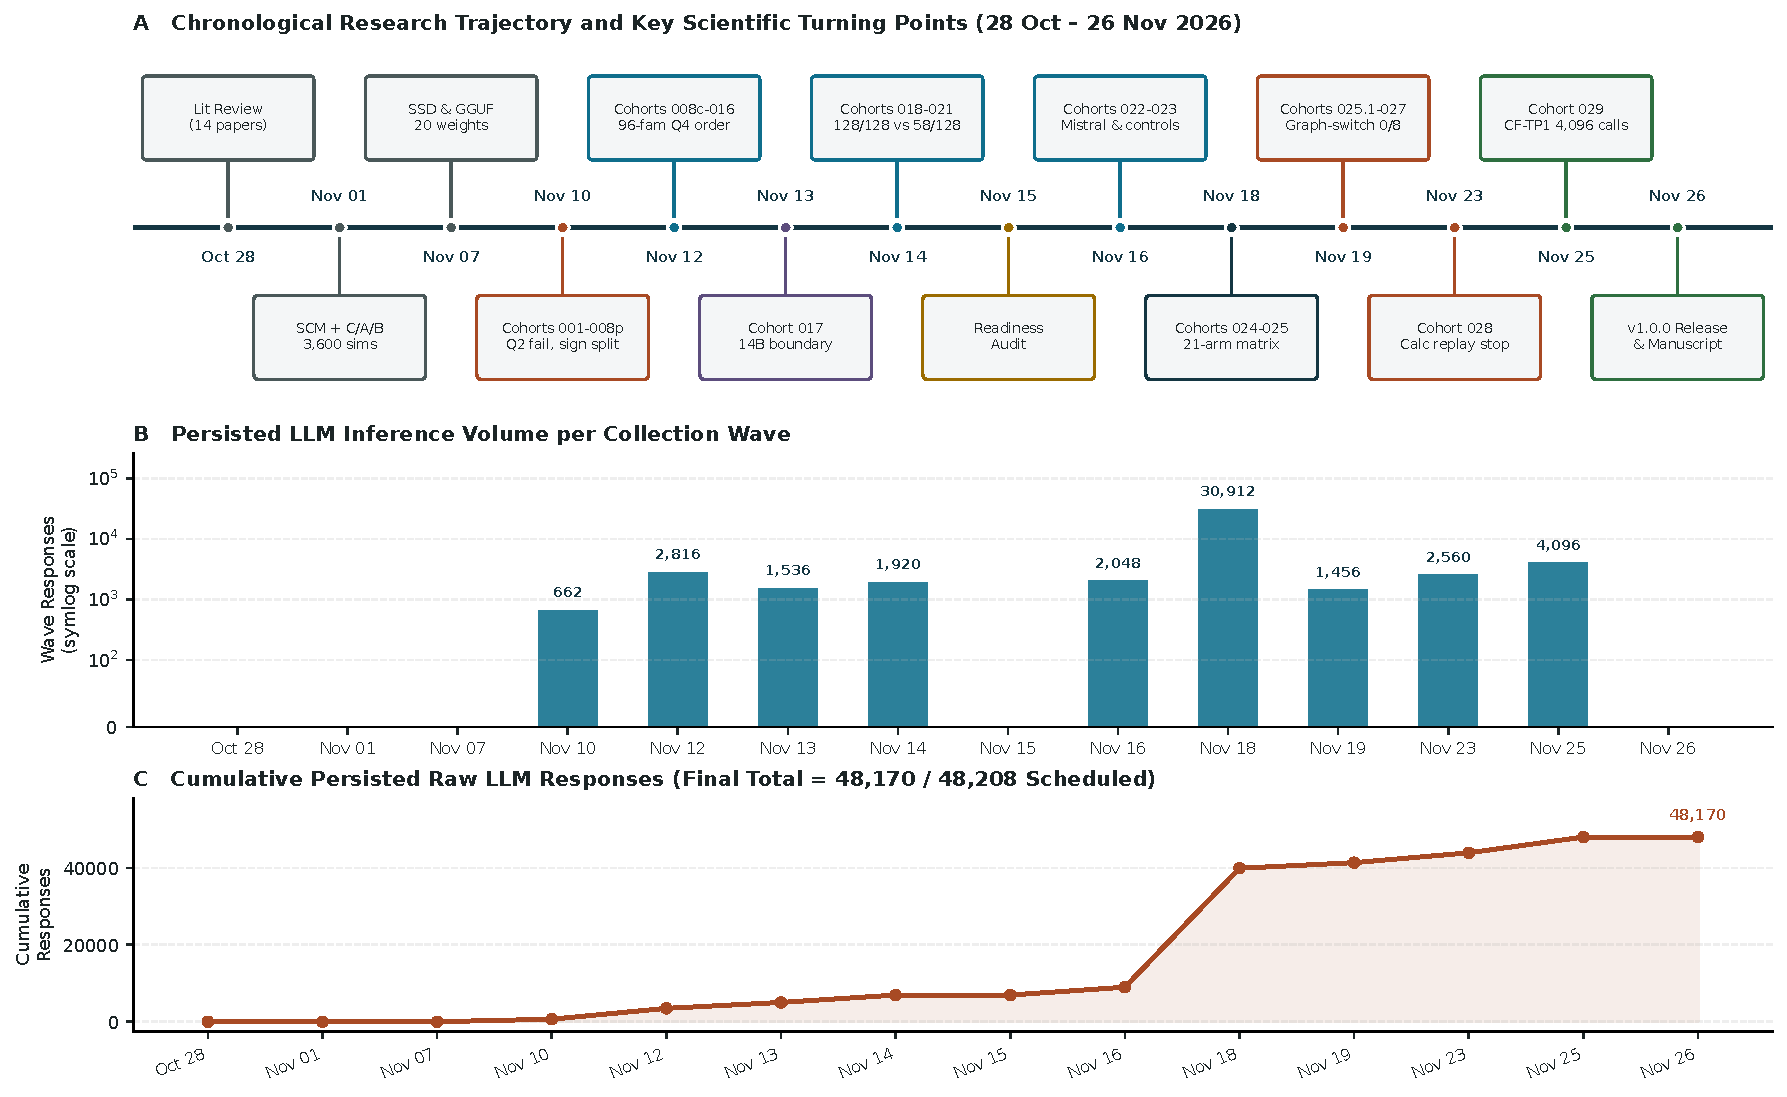
\includegraphics[width=\textwidth]{figures/fig01_research_timeline.pdf}
  \caption{Chronological overview of Project CausalFade across its 11 research phases (October 28 -- November 25, 2026; 320 commits, 30 cohorts plus pre-LLM synthetic validation, and $48{,}208$ scheduled inference requests).}
  \label{fig:timeline}
\end{figure}

\section{Why Causal Reasoning and Quantization Were Paired}

From a scientific standpoint, pairing causal identification with weight quantization was not an arbitrary combination of trendy topics; it rested on a plausible cognitive and computational asymmetry:

\begin{enumerate}
  \item \textbf{Associative shortcuts are cheap; causal adjustment is compositional.} In a confounded observational table where an upstream variable $Z$ (such as initial machine severity or patient baseline risk) drives both operator action $X$ and outcome $Y$, raw marginal association $\Prob(Y=1\mid X=1) - \Prob(Y=1\mid X=0)$ requires comparing two coarse summary tendencies. By contrast, Pearl's backdoor adjustment formula,
  \begin{equation}
    \Prob(Y=1 \mid \doop(X=x)) = \sum_{z \in \{0,1\}} \Prob(Y=1 \mid X=x, Z=z)\,\Prob(Z=z),
    \label{eq:origin_backdoor}
  \end{equation}
  requires (i) recognizing the causal graph structure $Z \to X, Z \to Y, X \to Y$, (ii) resisting the misleading marginal contrast, (iii) stratifying by $Z$, and (iv) weighting stratum-specific rates by target marginal shares $\Prob(Z=z)$ rather than treatment-conditioned shares $\Prob(Z=z\mid X=x)$.
  \item \textbf{Quantization introduces structured numerical perturbation into attention and MLP weights.} Post-training quantization maps continuous 16-bit floating-point weight blocks into coarse integer grids ($2$ to $8$ bits per weight). Recent work by \citet{marcuzzi2026bias} showed that quantization can amplify pre-existing distributional biases, while \citet{nwaiwu2025compressed} had published the only prior study explicitly combining quantization with causal benchmarks (\texttt{CLadder}), reporting accuracy drops at 4-bit precision.
  \item \textbf{The practical safety hazard of silent associative fallback.} If a heavily quantized model crashes into unreadable gibberish (as \texttt{Q2\_K} eventually did in Cohort~001), downstream software rejects the malformed output immediately. The far more dangerous failure mode hypothesized at project inception was \emph{silent schema-valid reversal}: a quantized model returning clean, syntactically valid JSON (\texttt{\{"activate": 1\}}) that confidently endorses a harmful action because quantization eroded multi-step backdoor adjustment while leaving associative pattern-matching intact.
\end{enumerate}

\section{The Initial Research Question and Prospective Hypothesis}

In its earliest formalization (\texttt{literature review/EXECUTIVE\_SUMMARY.md}, commit \texttt{4e2fe4f}, and \texttt{docs/STATISTICAL\_ANALYSIS\_PLAN.md}, commit \texttt{6ab18d2}), the project posed the following primary question:

\begin{definition}[Founding Research Question, October 28 -- November 1, 2026]
Does aggressive post-training quantization ($p \in \{\text{\texttt{Q8\_0}}, \text{\texttt{Q4\_K\_M}}, \text{\texttt{Q2\_K}}\}$) selectively increase an instruction-tuned LLM's vulnerability to confounding associations on interventional decision tasks relative to its unquantized half-precision (\texttt{F16}) reference?
\end{definition}

To operationalize this question, the researchers constructed synthetic binary structural causal worlds crossed in a $2\times 2$ design over two binary cues:
\begin{itemize}
  \item the \textbf{true interventional sign} $T \in \{0,1\}$, where $T=1$ iff $\ATE = \E[Y\mid \doop(X=1)] - \E[Y\mid \doop(X=0)] > 0$, and
  \item the \textbf{naive observational association sign} $S \in \{0,1\}$, where $S=1$ iff $\RD_{\mathrm{obs}} = \Prob(Y=1\mid X=1) - \Prob(Y=1\mid X=0) > 0$.
\end{itemize}
In \emph{aligned} items ($T = S$), causal adjustment and naive association recommend the same binary action. In \emph{conflict} items ($T \neq S$, a Simpson's reversal), naive association recommends the causally harmful action. Defining the within-precision conflict penalty as
\begin{equation}
  \mathrm{ConflictPenalty}(p) = \mathrm{Acc}_{\mathrm{aligned}}(p) - \mathrm{Acc}_{\mathrm{conflict}}(p),
\end{equation}
the founding prospective hypothesis (\texttt{H01} in our Hypothesis Ledger) predicted a positive quantization-by-conflict interaction:
\begin{equation}
  \Delta(p) = \mathrm{ConflictPenalty}(p) - \mathrm{ConflictPenalty}(\text{\texttt{F16}}) > 0.
  \label{eq:origin_delta}
\end{equation}

Notably, even at commit \texttt{4e2fe4f}, the researchers made a mature scoping decision (\texttt{D01} in \texttt{literature review/EXECUTIVE\_SUMMARY.md}): although early brainstorming had used the vivid metaphor of quantization ``severing causal circuits,'' the literature synthesis explicitly warned that behavioral prompts cannot identify internal neural circuits without activation patching or mechanistic interpretability. Accordingly, CausalFade prospectively restricted its claims to \emph{behavioral interventional competence} from day one.

\section{Original Assumptions---and How Reality Tested Them}

Looking back from the completed archive, the founding design rested on five implicit assumptions, every single one of which would soon fail empirically:

\begin{enumerate}
  \item \textbf{Assumption 1 (Reference Competence):} Unquantized \texttt{F16} instruction-tuned models ($3\text{B}$--$8\text{B}$) can reliably solve confounded interventional decision problems, providing a non-degenerate ceiling from which quantized models might ``fade.'' \emph{Reality:} Even \texttt{F16} models hovered near chance ($43\%$--$55\%$) on properly controlled causal decisions whenever surface shortcuts were removed.
  \item \textbf{Assumption 2 (Parser Neutrality):} Strict JSON schema enforcement treats \texttt{F16} and quantized models symmetrically. \emph{Reality:} In Cohort~001, \texttt{F16} wrapped valid JSON in Markdown fences $100\%$ of the time ($0/64$ strict accuracy), whereas \texttt{Q4\_K\_M} occasionally omitted fences, and in Cohort~024 \texttt{Llama-3.1-8B Q4\_K\_M} suffered $448$ length-capped verbose failures exclusively on noncausal controls.
  \item \textbf{Assumption 3 (Unbiased Action Priors):} Errors on conflict items reflect reliance on confounding association $S$ rather than unconditional preference for \texttt{activate=1} or \texttt{activate=0} or first-listed options. \emph{Reality:} Across nearly every cohort, models exhibited massive unconditional action biases (e.g., $63/64$ \texttt{activate=1} in Cohort~001 \texttt{F16}, $64/64$ \texttt{activate=0} in Cohort~002 \texttt{F16}, $995/1{,}024$ \texttt{activate=1} in Cohort~029 causal transfer, and $256/256$ first-option selection in Cohort~024 \texttt{Mistral F16}). Under a constant action policy, aligned and conflict accuracy are both exactly $50\%$, driving $\mathrm{ConflictPenalty}(p)$ artificially to $0$!
  \item \textbf{Assumption 4 (Internal Consistency Between Math and Action):} If a model computes the right negative ATE ($\widehat{\tau} < 0$), it will choose \texttt{activate=0}; if it computes $\widehat{\tau} > 0$, it will choose \texttt{activate=1}. \emph{Reality:} Cohorts~002, 006, and 007 uncovered a striking numeric-to-action dissociation in which \texttt{Qwen2.5-3B F16} computed the correct ATE sign on $61/64$ ($95.3\%$) of formula-assisted prompts while outputting \texttt{activate=0} on $64/64$ ($100\%$).
  \item \textbf{Assumption 5 (Absence of Numerical Magnitude Shortcuts):} Crossing $T$ and $S$ suffices to prevent noncausal shortcuts. \emph{Reality:} Unless numerical effect distributions are matched across studies and roles, deterministic source-blind rules (such as picking the smaller printed $|\text{on}-\text{off}|$ gap in Cohort~016) can achieve $100\%$ accuracy without reading causal provenance at all.
\end{enumerate}

\section{Original Objective vs.\ Eventual Scientific Contribution}

To read CausalFade honestly, one must hold two truths in view from the outset (Figure~\ref{fig:q_evolution}):

\begin{figure}[htbp]
  \centering
  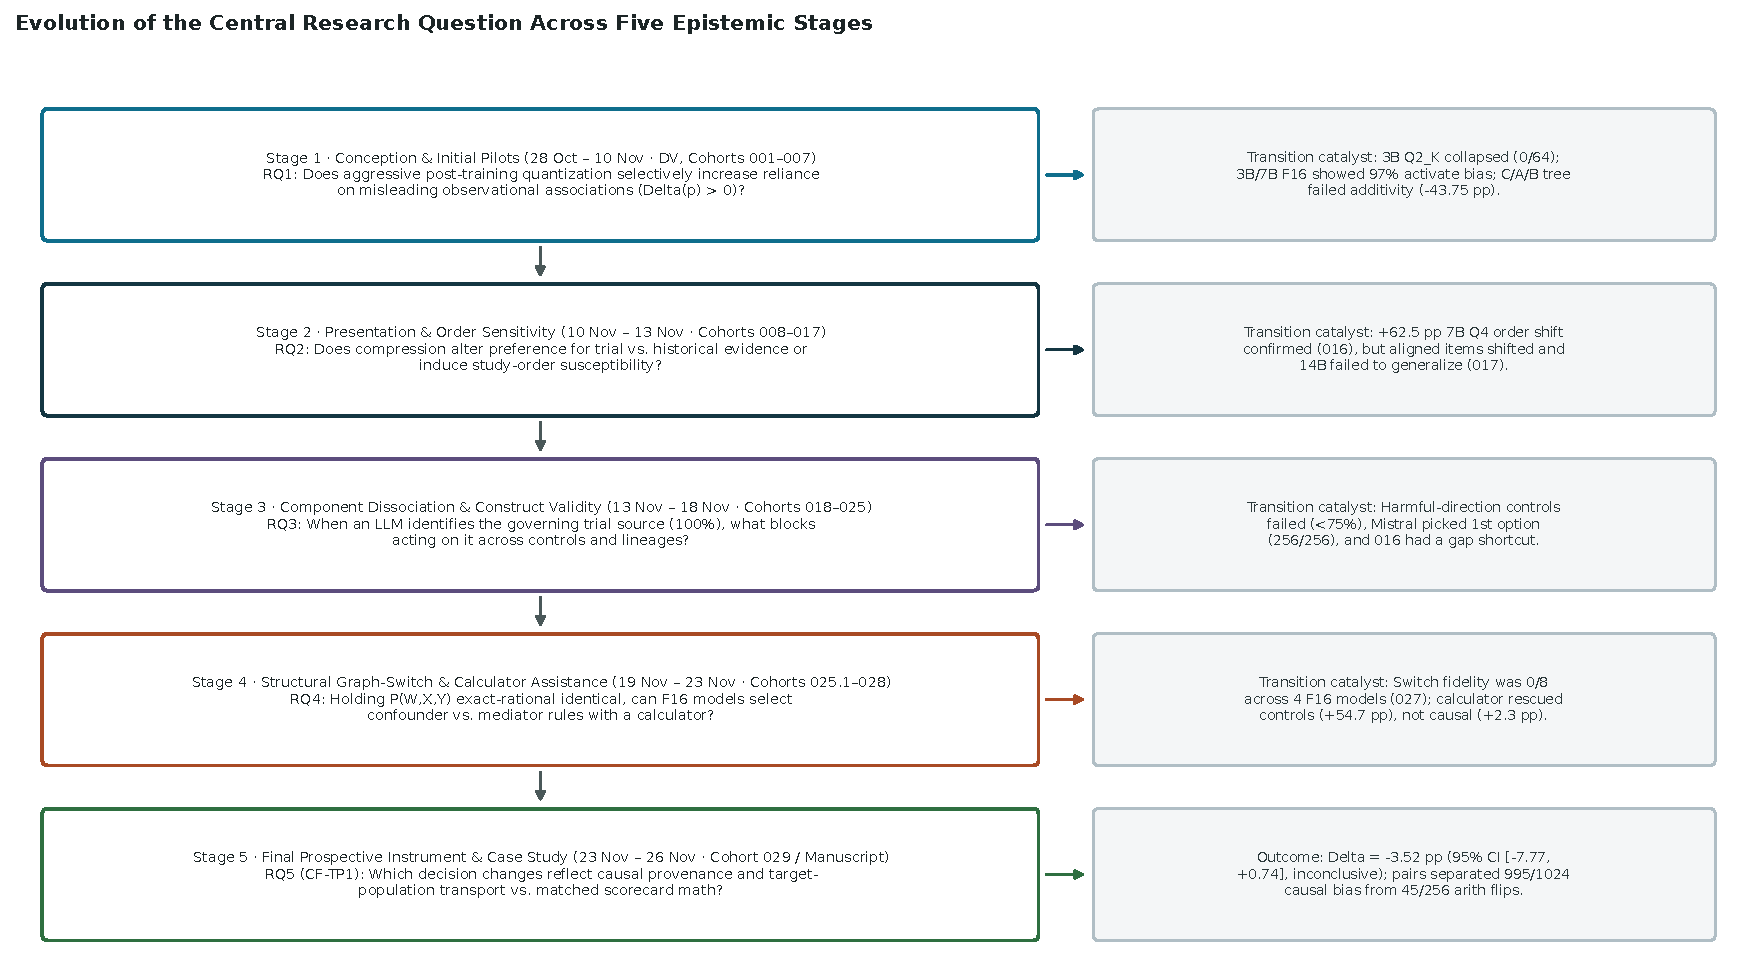
\includegraphics[width=\textwidth]{figures/fig02_question_evolution.pdf}
  \caption{Six-stage evolution of CausalFade's central research question, tracing how empirical anomalies forced the program from a quantization-degradation hypothesis (\texttt{RQ1}) to a general diagnostic framework for target-population causal transport and shortcut elimination (\texttt{RQ6}).}
  \label{fig:q_evolution}
\end{figure}

\begin{itemize}
  \item \textbf{What CausalFade originally hoped to demonstrate:} A clean dose--response curve showing that as GGUF precision drops from \texttt{F16} to \texttt{Q8\_0}, \texttt{Q4\_K\_M}, and \texttt{Q2\_K}, causal sensitivity $C$ decays while associative reliance $A$ rises.
  \item \textbf{What CausalFade actually discovered and contributed:} Selective quantization degradation of causal reasoning was \emph{not} established. Instead, through twenty-nine iterative cohorts of falsification and repair, CausalFade demonstrated why standard single-item LLM causal evaluations are pervasively confounded by action priors, option-order policies, numeric shortcuts, and baseline aggregation failures---culminating in \textbf{CF-TP1} (Cohort~029 and \texttt{manuscript/}), an exact-rational, $162$-policy-audited, paired reversal-and-retention benchmark for target-population causal transportability with matched noncausal arithmetic controls.
\end{itemize}

% =============================================================================
% Part I, Chapter 2: The Intellectual Foundation
% =============================================================================
\chapter{The Intellectual Foundation}\label{ch:literature}

Scientific projects do not arise in a vacuum, nor does their bibliography remain static while their research question transforms. A rigorous historical retrospective must distinguish between two bodies of literature that often become blended together in a finished journal article:
\begin{enumerate}
  \item \textbf{Contemporaneous foundational literature} that was actively read, summarized, and cited \emph{prior to or during} experimental design, directly shaping early hypotheses, metrics, and models; and
  \item \textbf{Retrospective positioning literature} incorporated later during benchmark hardening and manuscript preparation to situate newly discovered failure modes (such as option-order sensitivity, contrast-set scoring, and population transportability) within established research traditions.
\end{enumerate}

In Project CausalFade, Git provenance allows us to draw this boundary with unusual precision:
\begin{itemize}
  \item \textbf{Wave 1 (October 28, 2026, commit \texttt{4e2fe4f}):} Fourteen recent (2025--2026) papers on causal LLM benchmarks and quantized reasoning were downloaded, hashed in \texttt{literature review/paper\_manifest.json}, and analyzed in individual technical dossiers (\texttt{literature review/summaries/*.md}).
  \item \textbf{Wave 2 (November 1, 2026, commit \texttt{caf5b1d}):} Six foundational cognitive psychology, psychophysics, and psychometric modeling papers were added to \texttt{docs/references.bib} to ground the CNI-style multinomial processing tree (\texttt{design\_validation}, Cohort~005) and Signal Detection Theory (\texttt{SDT}) sensitivity/criterion decompositions.
  \item \textbf{Wave 3 (November 19--25, 2026, Cohort~029 and \texttt{manuscript/references.bib}):} Classical causal inference, transportability, shortcut-learning, long-context position bias, and finite-sample statistical references were integrated as the project pivoted to observationally equivalent graph switches (Cohorts~026--028) and the confirmatory \texttt{CF-TP1} target-population transport protocol (Cohort~029).
\end{itemize}

Below, we examine all thirty-nine verified publications in our monograph bibliography (\texttt{bibliography/references.bib}), organized into the nine intellectual pillars required to understand CausalFade. For each work, we document its research question, methodology, principal findings, limitations, provenance wave, documented influence on CausalFade, and how CausalFade diverged from or extended it.

% -----------------------------------------------------------------------------
\section{Foundational Causal Inference Literature}

\subsection{Pearl (2009) --- \emph{Causality: Models, Reasoning, and Inference} \citep{pearl2009causality}}
\begin{itemize}
  \item \textbf{Bibliographic Record:} Judea Pearl, \emph{Causality: Models, Reasoning, and Inference}, 2nd ed., Cambridge University Press, 2009 (ISBN 978-0521895606). \emph{Provenance:} Implicit mathematical foundation from commit \texttt{4e2fe4f}; formally cited in \texttt{manuscript/references.bib}.
  \item \textbf{Research Question \& Methodology:} How can causal claims, interventions, and counterfactuals be formalized mathematically rather than treated merely as informal interpretations of statistical associations? Introduces Structural Causal Models (SCMs), Directed Acyclic Graphs (DAGs), $d$-separation, the intervention operator $\doop(X=x)$, the backdoor and frontdoor criteria, and the three-rung Ladder of Causation (Rung~1 association $\Prob(y\mid x)$, Rung~2 intervention $\Prob(y\mid \doop(x))$, Rung~3 counterfactuals $\Prob(y_x\mid x', y')$).
  \item \textbf{Principal Findings \& Limitations:} Establishes sound and complete graphical and algebraic rules ($\doop$-calculus) for deciding when interventional distributions are identifiable from observational distributions. Assumes exact knowledge of qualitative causal structure and positivity; finite-sample estimation and behavioral execution by bounded agents lie outside its axiomatic scope.
  \item \textbf{Influence \& Extension in CausalFade:} Provided the exact mathematical target for every causal task in CausalFade: backdoor standardization in Cohorts~001--011, interventional vs.\ observational source dominance in Cohorts~012--025, confounder vs.\ mediator identification in Cohorts~026--028, and group-standardized causal effects in Cohort~029. CausalFade extended Pearl's identification theory into an \emph{empirical behavioral diagnostic} testing whether bounded language models actually switch estimation formulas when causal structure or target composition changes.
\end{itemize}

\subsection{Rubin (1974) --- Potential Outcomes in Randomized and Nonrandomized Studies \citep{rubin1974estimating}}
\begin{itemize}
  \item \textbf{Bibliographic Record:} Donald B. Rubin, ``Estimating Causal Effects of Treatments in Randomized and Nonrandomized Studies,'' \emph{Journal of Educational Psychology}, 66(5):688--701, 1974 (\texttt{doi:10.1037/h0037350}). \emph{Provenance:} Wave~3 positioning (\texttt{manuscript/references.bib}).
  \item \textbf{Research Question \& Methodology:} Formalizes unit-level causal effects $Y_i(1) - Y_i(0)$ and analyzes when randomized trials versus nonrandomized observational studies yield unbiased estimates of average treatment effects across a target population.
  \item \textbf{Principal Findings \& Limitations:} Demonstrates why random assignment eliminates unmeasured baseline confounding in expectation, whereas nonrandomized operator assignment requires Measuring and adjusting for all confounding covariates. Does not provide graphical criteria for covariate selection (where conditioning on post-treatment mediators or colliders induces bias).
  \item \textbf{Influence \& Extension in CausalFade:} Directly underpins the two-study paradigm introduced in Cohort~012 and refined through Cohort~029, where a randomized study identifies causal stratum effects despite unmeasured operator risk $U$ that corrupts a parallel historical study.
\end{itemize}

% -----------------------------------------------------------------------------
\section{Causal Reasoning in Language Models}

\subsection{Jin et al.\ (2023) --- \texttt{CLadder}: Assessing Causal Reasoning in Language Models \citep{jin2023cladder}}
\begin{itemize}
  \item \textbf{Bibliographic Record:} Zhijing Jin et al., ``CLadder: Assessing Causal Reasoning in Language Models,'' \emph{Advances in Neural Information Processing Systems (NeurIPS)}, 36:31038--31065, 2023. \emph{Provenance:} Referenced across Wave~1 summaries (via \citealt{nwaiwu2025compressed,yu2025causaleval}) and formally cited in Wave~3 (\texttt{manuscript/references.bib}).
  \item \textbf{Research Question \& Methodology:} Can LLMs solve formal causal inference queries across all three rungs of Pearl's Ladder? Generates $10{,}000+$ natural-language causal queries paired with symbolic ground truth from underlying SCMs and evaluates models with and without chain-of-thought (\texttt{CausalCoT}) prompting.
  \item \textbf{Principal Findings \& Limitations:} Off-the-shelf LLMs struggle substantially on formal backdoor, frontdoor, and counterfactual queries, though structured step-by-step prompting improves performance. Limitations: Single-item binary yes/no scoring is vulnerable to label/prior imbalances and verbal template shortcuts, and \texttt{CLadder} lacks matched noncausal arithmetic controls on identical numerical tables.
  \item \textbf{Influence \& Extension in CausalFade:} Inspired Cohort~001's fictional machine framing (avoiding memorized world knowledge) and numerical backdoor tables. CausalFade went substantially beyond \texttt{CLadder} by adding orthogonal cue crossing, matched noncausal scorecard controls, deterministic $162$-policy shortcut audits, and paired reversal/retention scoring.
\end{itemize}

\subsection{K\i c\i man et al.\ (2023) --- Causal Reasoning and Large Language Models \citep{kiciman2023causal}}
\begin{itemize}
  \item \textbf{Bibliographic Record:} Emre K\i c\i man, Robert Ness, Amit Sharma, and Chenhao Tan, ``Causal Reasoning and Large Language Models: Opening a New Frontier for Causality,'' \emph{arXiv:2305.00050}, 2023. \emph{Provenance:} Wave~3 positioning.
  \item \textbf{Research Question \& Methodology:} Evaluates early frontier LLMs on pairwise causal discovery, counterfactual narrative judgment, and commonsense causal attribution benchmarks.
  \item \textbf{Principal Findings \& Limitations:} Reports surprisingly high accuracy on semantic causal direction benchmarks, sparking widespread optimism about LLM causal capabilities. However, performance relied heavily on pre-trained domain semantics rather than formal identification from quantitative data, leaving open whether models could reason causally when semantic priors were neutralized.
  \item \textbf{Influence \& Extension in CausalFade:} Served as the foil for CausalFade's anti-memorization design: CausalFade deliberately stripped real-world semantic cues (using fictional machine settings and abstract ``Amber/Blue'' strata) precisely to prevent domain-knowledge lookup from masquerading as formal causal inference.
\end{itemize}

\subsection{Yu et al.\ (2025) --- \texttt{CausalEval}: Towards Better Causal Reasoning in Language Models \citep{yu2025causaleval}}
\begin{itemize}
  \item \textbf{Bibliographic Record:} Longxuan Yu et al., ``CausalEval: Towards Better Causal Reasoning in Language Models,'' \emph{Proceedings of NAACL-HLT 2025 (Volume 1: Long Papers)}, pp.~12512--12540, 2025 (\texttt{doi:10.18653/v1/2025.naacl-long.622}). \emph{Provenance:} Wave~3 positioning.
  \item \textbf{Research Question \& Methodology:} Separates knowledge-driven causal questions from formal rule-driven causal inference tasks across multiple LLM families.
  \item \textbf{Principal Findings \& Limitations:} Shows that LLMs perform much worse on formal structural causal tasks than on commonsense causal questions, and exhibit sensitivity to surface phrasing. Lacks paired interventional switch scoring and quantization/control baselines.
  \item \textbf{Influence \& Extension in CausalFade:} Reinforced the distinction between archive prompt wording and natural-prose transfer wording implemented as an explicit crossed factor in Cohort~029 (\texttt{CF-TP1}).
\end{itemize}

\subsection{Ma (2025) --- Causal Inference with Large Language Model: A Survey \citep{ma2025survey}}
\begin{itemize}
  \item \textbf{Bibliographic Record:} Jing Ma, ``Causal Inference with Large Language Model: A Survey,'' \emph{Findings of the Association for Computational Linguistics: NAACL 2025}, pp.~5901--5913, 2025 (\texttt{doi:10.18653/v1/2025.findings-naacl.327}). \emph{Provenance:} Wave~3 positioning.
  \item \textbf{Research Question \& Methodology:} Taxonomizes roles of LLMs in causality (causal discovery prior, treatment effect estimator, natural-language confounder adjuster, and benchmark subject).
  \item \textbf{Principal Findings \& Limitations:} Identifies benchmark contamination, prompt brittleness, and lack of theoretical guarantees as central open challenges. Survey scope without new empirical experiments.
  \item \textbf{Influence \& Extension in CausalFade:} Contextualized CausalFade's final methodological contribution within broader evaluation pitfalls surveyed across NLP and causal AI.
\end{itemize}

\subsection{Wang, Zhu, and Li (2026) --- \texttt{CausalFlip}: Beyond Semantic Matching \citep{wang2026causalflip}}
\begin{itemize}
  \item \textbf{Bibliographic Record:} Yuzhe Wang, Yaochen Zhu, and Jundong Li, ``CausalFlip: A Benchmark for LLM Causal Judgment Beyond Semantic Matching,'' \emph{arXiv:2602.20094v2}, 2026. \emph{Provenance:} Wave~1 (\texttt{literature review/summaries/02\_causalflip.md}, commit \texttt{4e2fe4f}).
  \item \textbf{Research Question \& Methodology:} Do LLMs answer causal questions by genuine structural reasoning or by matching semantic associations? Constructs paired scenarios where minimal structural edits flip the true causal relation while preserving surface lexical similarity.
  \item \textbf{Principal Findings \& Limitations:} Demonstrates steep accuracy drops when structural flips contradict semantic expectations. Evaluates qualitative judgment rather than quantitative interventional standardization or compressed local models.
  \item \textbf{Influence \& Extension in CausalFade:} Directly inspired CausalFade's insistence on \emph{paired structural flips}---first in Cohort~001's $2\times 2$ $(T,S)$ family quartets, then in Cohort~026--028's confounder-vs.-mediator flips on identical $P(W,X,Y)$ tables, and finally in Cohort~029's target-mix switch pairs.
\end{itemize}

\subsection{Sawarni, Tan, and Syrgkanis (2026) --- \texttt{CausalReasoningBenchmark} \citep{sawarni2026crb}}
\begin{itemize}
  \item \textbf{Bibliographic Record:} Ayush Sawarni, Jiyuan Tan, and Vasilis Syrgkanis, ``CausalReasoningBenchmark: A Real-World Benchmark for Disentangled Evaluation of Causal Identification and Estimation,'' \emph{arXiv:2602.20571v3}, 2026. \emph{Provenance:} Wave~1 (\texttt{literature review/summaries/07\_causal\_reasoning\_benchmark.md}, commit \texttt{4e2fe4f}).
  \item \textbf{Research Question \& Methodology:} Disentangles two stages of applied causal inference: (1) \emph{causal identification} (choosing valid adjustment sets/estimators from a graph or domain story) and (2) \emph{statistical estimation} (computing numerical estimates from data). Evaluates coding/data-science LLM workflows on 143 real-world datasets.
  \item \textbf{Principal Findings \& Limitations:} Shows that identification errors and estimation implementation bugs fail independently and must not be collapsed into a single composite score. Relies on real-world empirical studies (potential pre-training familiarity) and full-precision cloud models.
  \item \textbf{Influence \& Extension in CausalFade:} Directly motivated Cohort~001's multi-field schema (\texttt{adjustment\_set}, \texttt{ate\_estimate}, \texttt{activate}), Cohort~006's formula-assisted separation of identification from calculation, and Cohort~028's \texttt{System B} vs.\ \texttt{System C} deterministic calculator ablation, which cleanly proved that offloading estimation rescued noncausal tasks ($+54.69\pp$ in Qwen) while leaving causal identification near chance ($68/128$).
\end{itemize}

% -----------------------------------------------------------------------------
\section{Model Quantization and Compression}

\subsection{Nwaiwu, Jongsawat, and Tungkasthan (2025) --- Compressed Causal Reasoning \citep{nwaiwu2025compressed}}
\begin{itemize}
  \item \textbf{Bibliographic Record:} Steve Nwaiwu, Nipat Jongsawat, and Anucha Tungkasthan, ``Compressed Causal Reasoning: Quantization and GraphRAG Effects on Interventional and Counterfactual Accuracy,'' \emph{arXiv:2512.13725v2}, 2025. \emph{Provenance:} Wave~1 (\texttt{literature review/summaries/01\_compressed\_causal\_reasoning.md}, commit \texttt{4e2fe4f})---the single closest prior study to CausalFade's initial premise.
  \item \textbf{Research Question \& Methodology:} Evaluates quantized open-weight LLMs (4-bit and 8-bit) with and without GraphRAG retrieval on interventional and counterfactual questions adapted from \texttt{CLadder}.
  \item \textbf{Principal Findings \& Limitations:} Reports modest accuracy reductions under 4-bit quantization partially mitigated by external graph retrieval. Crucially, however, as noted in CausalFade's Wave~1 summary, it evaluated passive single-item question answering without matched noncausal arithmetic controls, without crossing causal and associative signs to control for default yes/no bias, and without exploring sub-4-bit GGUF formats (\texttt{Q3\_K\_M}, \texttt{Q2\_K}).
  \item \textbf{Influence \& Extension in CausalFade:} Provided the direct springboard for CausalFade's founding gap claim. Ironically, CausalFade's deeper controls later showed that single-item accuracy shifts of the kind studied in \citet{nwaiwu2025compressed} are heavily confounded by formatting invalidity, action priors, and baseline noncausal failures.
\end{itemize}

\subsection{Liu et al.\ (2025) --- Quantization Hurts Reasoning? \citep{liu2025hurts}}
\begin{itemize}
  \item \textbf{Bibliographic Record:} Ruikang Liu et al., ``Quantization Hurts Reasoning? An Empirical Study on Quantized Reasoning Models,'' \emph{arXiv:2504.04823v2 (COLM 2025)}, 2025. \emph{Provenance:} Wave~1 (\texttt{09\_quantization\_hurts\_reasoning.md}).
  \item \textbf{Research Question \& Methodology:} Systematically benchmarks weight, KV-cache, and activation quantization (W8A8, W4, W3, W2) across reasoning-distilled Qwen and Llama families ($1.5\text{B}$--$70\text{B}$) on mathematical and coding benchmarks.
  \item \textbf{Principal Findings \& Limitations:} Finds near-lossless performance at 8-bit, mild degradation at 4-bit that widens on smaller ($1.5\text{B}$--$3\text{B}$) models, and severe collapse at $\le 3$-bit precision. Does not test causal confounding or decision bias.
  \item \textbf{Influence \& Extension in CausalFade:} Directly informed CausalFade's choice of the \texttt{Qwen2.5} and \texttt{Llama-3.1} model families and the initial quantization ladder (\texttt{F16}, \texttt{Q8\_0}, \texttt{Q4\_K\_M}, \texttt{Q2\_K}), accurately foreshadowing both the \texttt{3B Q4\_K\_M} formula-execution drop in Cohorts~006--007 and the catastrophic \texttt{Q2\_K} collapse in Cohort~001.
\end{itemize}

\subsection{Li et al.\ (2025) --- Quantization Meets Reasoning \citep{li2025meets}}
\begin{itemize}
  \item \textbf{Bibliographic Record:} Zhen Li et al., ``Quantization Meets Reasoning: Exploring and Mitigating Degradation of Low-Bit LLMs in Mathematical Reasoning,'' \emph{arXiv:2505.11574v4}, 2025. \emph{Provenance:} Wave~1 (\texttt{10\_quantization\_meets\_reasoning.md}).
  \item \textbf{Research Question \& Methodology:} Investigates why low-bit PTQ degrades multi-step mathematical chains through error accumulation across reasoning steps.
  \item \textbf{Principal Findings \& Limitations:} Shows that small logit perturbations compound over sequential arithmetic steps, causing trajectory divergence even when single-step recall appears intact. Limited to mathematical word problems.
  \item \textbf{Influence \& Extension in CausalFade:} Motivated testing whether causal failures in quantized models were actually disguised multi-step arithmetic errors---leading directly to Cohort~006's formula-assisted condition, Cohort~024's matched noncausal scorecard controls, and Cohort~029's arithmetic baseline.
\end{itemize}

\subsection{Zhang et al.\ (2025) --- When Reasoning Meets Compression \citep{zhang2025compression}}
\begin{itemize}
  \item \textbf{Bibliographic Record:} Nan Zhang et al., ``When Reasoning Meets Compression: Understanding the Effects of LLMs Compression on Large Reasoning Models,'' \emph{arXiv:2504.02010v3 (ICLR 2026)}, 2025. \emph{Provenance:} Wave~1 (\texttt{11\_when\_reasoning\_meets\_compression.md}).
  \item \textbf{Research Question \& Methodology:} Compares quantization, pruning, and distillation on reasoning models across difficulty tiers and output-length budgets.
  \item \textbf{Principal Findings \& Limitations:} Demonstrates that compression interacts strongly with generation-length caps: compressed models frequently require longer, more repetitive chains and suffer premature truncation under tight \texttt{max\_tokens} budgets.
  \item \textbf{Influence \& Extension in CausalFade:} Directly explained two major operational artifacts in CausalFade: \texttt{3B Q2\_K} hitting \texttt{finish\_reason="length"} on $64/64$ items in Cohort~001, and \texttt{Llama-3.1-8B Q4\_K\_M} hitting length caps on $448$ noncausal control prompts in Cohort~024 when ignoring JSON-only instructions.
\end{itemize}

\subsection{Lian et al.\ (2026) --- Quantization Inflates Reasoning \citep{lian2026inflates}}
\begin{itemize}
  \item \textbf{Bibliographic Record:} Xinyu Lian et al., ``Quantization Inflates Reasoning: Token Inflation as a Hidden Cost of Low-Bit Reasoning Models,'' \emph{arXiv:2606.25519v2}, 2026. \emph{Provenance:} Wave~1 (\texttt{08\_quantization\_inflates\_reasoning.md}).
  \item \textbf{Research Question \& Methodology:} Quantifies ``token inflation''---the tendency of low-bit quantized models to emit substantially more tokens, repetitive self-corrections, or verbose preambles before terminating.
  \item \textbf{Principal Findings \& Limitations:} Shows that low-bit quantization degrades stopping calibration and format conciseness, inflating completion length by $20\%$--$200\%$ and causing truncation under fixed token budgets.
  \item \textbf{Influence \& Extension in CausalFade:} Motivated logging \texttt{completion\_tokens}, \texttt{finish\_reason}, and parser failure categories separately from semantic accuracy across all cohorts, which proved essential for diagnosing Cohort~024's \texttt{Llama Q4\_K\_M} control-task truncation anomaly.
\end{itemize}

\subsection{Alimaskina et al.\ (2026) --- Extreme Low-Bit Inference in Reasoning Models \citep{alimaskina2026extreme}}
\begin{itemize}
  \item \textbf{Bibliographic Record:} Ekaterina Alimaskina et al., ``Extreme Low-Bit Inference in Reasoning Models: Failure Modes and Targeted Recovery,'' \emph{arXiv:2606.02011v1}, 2026. \emph{Provenance:} Wave~1 (\texttt{12\_extreme\_low\_bit\_reasoning.md}).
  \item \textbf{Research Question \& Methodology:} Catalogs taxonomy of failure modes at $1.5$--$3$ bits per weight (token looping, punctuation collapse, instruction amnesia) and tests mixed-precision recovery.
  \item \textbf{Principal Findings \& Limitations:} Distinguishes catastrophic syntactic/looping collapse at $\le 2.5\;\BPW$ from subtle semantic errors at $4\;\BPW$.
  \item \textbf{Influence \& Extension in CausalFade:} Provided the diagnostic lens for Cohorts~001, 003, and 004, where \texttt{Qwen2.5-3B Q2\_K} degenerated into numeric/quote token loops (\texttt{"43)366323..."}), prompting CausalFade to test whether \texttt{Q3\_K\_M} (Cohort~004) or larger $7\text{B}$ lineages (Cohort~024) remained schema-viable at extreme compression.
\end{itemize}

\subsection{Lv et al.\ (2026) --- Low-Bit Quantization-Aware Training for Reasoning LLMs \citep{lv2026reasoningqat}}
\begin{itemize}
  \item \textbf{Bibliographic Record:} Keyu Lv et al., ``What Makes Low-Bit Quantization-Aware Training Work for Reasoning LLMs? A Systematic Study,'' \emph{arXiv:2601.14888v1}, 2026. \emph{Provenance:} Wave~1 (\texttt{13\_low\_bit\_qat\_reasoning.md}).
  \item \textbf{Research Question \& Methodology:} Compares post-training quantization (PTQ) against quantization-aware training (QAT) on multi-step reasoning benchmarks.
  \item \textbf{Principal Findings \& Limitations:} Shows naive uniform/block PTQ without calibration data (such as uncalibrated \texttt{llama-quantize} runs) suffers sharper degradation below 4 bits than QAT or importance-matrix (\texttt{imatrix}) calibrated PTQ.
  \item \textbf{Influence \& Extension in CausalFade:} Motivated CausalFade's meticulous provenance recording (\texttt{docs/SSD\_ASSET\_REUSE.md}), explicitly documenting that the local GGUF conversions used \texttt{llama-quantize} build \texttt{b12176} \emph{without} an importance matrix so readers would not confuse uncalibrated PTQ collapse at \texttt{Q2\_K} with optimal QAT performance.
\end{itemize}

\subsection{Vaish et al.\ (2026) --- \texttt{PRISM}: Parametric Recall Degradation in Quantized LLMs \citep{vaish2026prism}}
\begin{itemize}
  \item \textbf{Bibliographic Record:} Swastik Vaish, Arpit Singh Gautam, Varun Tiwari, and Jitendra Singh Yadav, ``PRISM a diagnostic framework for parametric recall degradation in quantized large language models,'' \emph{Discover Computing}, 29(1):700, 2026 (\texttt{doi:10.1007/s10791-026-10580-5}). \emph{Provenance:} Wave~1 (\texttt{14\_prism\_quantization\_recall.md}).
  \item \textbf{Research Question \& Methodology:} Separates factual parametric memory loss from in-context reasoning loss across quantized LLMs.
  \item \textbf{Principal Findings \& Limitations:} Demonstrates that quantization disproportionately erodes rare parametric facts stored in weights before degrading in-context copying.
  \item \textbf{Influence \& Extension in CausalFade:} Reinforced CausalFade's decision to make every causal task \emph{self-contained in context} (supplying exact numerical tables and explicit graph assumptions in the prompt) so parametric memory loss could not be conflated with causal reasoning failure.
\end{itemize}

\subsection{Marcuzzi et al.\ (2026) --- How Quantization Shapes Bias in Large Language Models \citep{marcuzzi2026bias}}
\begin{itemize}
  \item \textbf{Bibliographic Record:} Federico Marcuzzi, Xuefei Ning, Roy Schwartz, and Iryna Gurevych, ``How Quantization Shapes Bias in Large Language Models,'' \emph{Proceedings of EACL 2026 (Volume 1: Long Papers)}, 2026 (\texttt{doi:10.18653/v1/2026.eacl-long.17}). \emph{Provenance:} Wave~2 (\texttt{docs/references.bib}, commit \texttt{caf5b1d}).
  \item \textbf{Research Question \& Methodology:} Examines how weight and activation quantization alter social, lexical, and label-selection biases across instruction-tuned LLMs.
  \item \textbf{Principal Findings \& Limitations:} Proves that quantization frequently shifts output priors and response tendencies rather than uniformly adding symmetric noise---meaning accuracy on unbalanced or non-crossed benchmarks can artificially rise or fall when a quantized model becomes more biased toward one response label.
  \item \textbf{Influence \& Extension in CausalFade:} Crucially anticipated CausalFade's discovery in Cohorts~005, 011, and 024 that \texttt{Q4\_K\_M} could exhibit a \emph{smaller} apparent conflict penalty than \texttt{F16} simply because quantization shifted unconditional \texttt{activate=1} / \texttt{decline} bias!
\end{itemize}

\subsection{Lyu et al.\ (2026) --- Task Value of Precision Upgrades in Closed-Loop Agents \citep{lyu2026precision}}
\begin{itemize}
  \item \textbf{Bibliographic Record:} Sicheng Lyu et al., ``Measuring the Task Value of Precision Upgrades in Closed-Loop Agents,'' \emph{arXiv:2610.24346}, 2026. \emph{Provenance:} Wave~1 (\texttt{06\_precision\_upgrades\_agents.md}).
  \item \textbf{Research Question \& Methodology:} Evaluates when upgrading precision from 4-bit to 8-bit/16-bit materially improves decision utility in sequential agent loops.
  \item \textbf{Principal Findings \& Limitations:} Finds that precision upgrades often yield negligible end-to-end decision gains unless the underlying full-precision agent already possesses non-degenerate task competence.
  \item \textbf{Influence \& Extension in CausalFade:} Foreshadowed CausalFade's overarching empirical outcome: when \texttt{F16} models themselves lack robust causal switching ($0/8$ in Cohort~027; $<75\%$ controls in Cohort~024), comparing \texttt{Q4\_K\_M} against \texttt{F16} measures shifts between degenerate policies rather than loss of causal competence.
\end{itemize}

% -----------------------------------------------------------------------------
\section{Reasoning Evaluation, Process Dissociation, and Psychometrics}

\subsection{Jacoby (1991) --- Process Dissociation Framework \citep{jacoby1991process}}
\begin{itemize}
  \item \textbf{Bibliographic Record:} Larry L. Jacoby, ``A Process Dissociation Framework: Separating Automatic from Intentional Uses of Memory,'' \emph{Journal of Memory and Language}, 30(5):513--541, 1991 (\texttt{doi:10.1016/0749-596X(91)90025-F}). \emph{Provenance:} Wave~2 (\texttt{docs/references.bib}, commit \texttt{caf5b1d}).
  \item \textbf{Research Question \& Methodology:} Introduces the method of \emph{inclusion} (automatic and intentional processes act in concert) versus \emph{exclusion} (intentional control opposes automatic habit) to algebraically separate controlled processing from automatic fallback.
  \item \textbf{Principal Findings \& Limitations:} Proves that comparing aligned ($T=S$) and conflict ($T\neq S$) conditions alone cannot separate intentional control from automatic bias unless response bias is also controlled; assumes stochastic independence and parameter invariance across inclusion and exclusion cells.
  \item \textbf{Influence \& Extension in CausalFade:} Provided the exact conceptual blueprint for crossing interventional direction $T$ with associative direction $S$ in \texttt{design\_validation} and Cohorts~001--011, and also predicted the exact invariance failure observed in Cohort~005 when \texttt{F16} violated cross-cell parameter homogeneity.
\end{itemize}

\subsection{Gawronski et al.\ (2017) --- The CNI Model of Moral Decision-Making \citep{gawronski2017cni}}
\begin{itemize}
  \item \textbf{Bibliographic Record:} Bertram Gawronski, Joel Armstrong, Paul Conway, Rebecca Friesdorf, and Mandy H{\"u}tter, ``Consequences, Norms, and Generalized Inaction in Moral Dilemmas: The CNI Model of Moral Decision-Making,'' \emph{Journal of Personality and Social Psychology}, 113(3):343--376, 2017 (\texttt{doi:10.1037/pspa0000086}). \emph{Provenance:} Wave~2 (\texttt{docs/references.bib}, commit \texttt{caf5b1d}).
  \item \textbf{Research Question \& Methodology:} Uses a $2\times 2$ multinomial processing tree with three parameters---Consequences ($C$), Norms ($N$), and generalized Inaction/action preference ($I$)---across four dilemma types ($1$ degree of freedom for goodness-of-fit testing).
  \item \textbf{Principal Findings \& Limitations:} Separates genuine sensitivity to two competing rules from unconditional action/inaction bias. Assumes sequential conditional hierarchy ($C$ dominates $N$, which dominates $I$) and homogeneous parameters across all four cells.
  \item \textbf{Influence \& Extension in CausalFade:} Directly adapted in \texttt{causalfade/cab\_tree.py} as the Causal/Associative/Bias ($C/A/B$) processing tree: $\Prob(\text{act}=1\mid T,S) = C T + (1-C)[A S + (1-A) B]$. Critically, CausalFade tested Gawronski's $1$-df goodness-of-fit constraint rather than assuming it, discovering in Cohort~005 that \texttt{Qwen2.5-3B F16} violated tree additivity by $-43.75\pp$ and retiring $C/A/B$ latent-route claims immediately (\texttt{D05}).
\end{itemize}

\subsection{Heck, Arnold, and Arnold (2018) --- \texttt{TreeBUGS} and MPT Diagnostics \citep{heck2018treebugs}}
\begin{itemize}
  \item \textbf{Bibliographic Record:} Daniel W. Heck, Nina R. Arnold, and Denis Arnold, ``TreeBUGS: An R Package for Hierarchical Multinomial-Processing-Tree Modeling,'' \emph{Behavior Research Methods}, 50:264--284, 2018 (\texttt{doi:10.3758/s13428-017-0869-7}). \emph{Provenance:} Wave~2 (\texttt{docs/references.bib}).
  \item \textbf{Research Question \& Methodology:} Develops hierarchical estimation, parameter-recovery checks, and parametric bootstrap deviance diagnostics for multinomial processing trees (MPTs), emphasizing item/family heterogeneity and simplex boundary behavior.
  \item \textbf{Principal Findings \& Limitations:} Warns that pooling heterogeneous items into an aggregate MPT biases parameter estimates and that conditional branch parameters become weakly identified when upstream parameters approach $1$ or sample sizes are small.
  \item \textbf{Influence \& Extension in CausalFade:} Directly guided \texttt{results/design\_validation/VALIDATION\_REPORT.md} (3,600 synthetic datasets testing $C\to 1$ boundary nonconvergence and parametric bootstrap $G^2$ deviance).
\end{itemize}

\subsection{Wu and Deng (2025) --- Applying CNI Trees to LLM Judgments \citep{wuDeng2025counts}}
\begin{itemize}
  \item \textbf{Bibliographic Record:} Wenya Wu and Weihong Deng, ``What Counts Underlying LLMs' Moral Dilemma Judgments?,'' \emph{Proceedings of the Fourth Workshop on NLP for Positive Impact (NLP4PI)}, pp.~144--150, 2025 (\texttt{doi:10.18653/v1/2025.nlp4pi-1.12}). \emph{Provenance:} Wave~2 (\texttt{docs/references.bib}).
  \item \textbf{Research Question \& Methodology:} Applies Gawronski's CNI multinomial processing tree directly to LLM binary responses to separate rule sensitivity from action bias.
  \item \textbf{Principal Findings \& Limitations:} Demonstrates that LLMs harbor strong generalized action/inaction biases, but applies the CNI tree without testing observational equivalence against continuous logistic cue integration.
  \item \textbf{Influence \& Extension in CausalFade:} CausalFade explicitly audited this gap in \texttt{design\_validation}, proving mathematically and via simulation that symmetric additive logistic integration is observationally equivalent to the 3-parameter CNI/$C/A/B$ tree on 4 cells ($p_{\text{boot}} = 0.433$), preventing over-interpretation of tree parameters as sequential internal mechanisms.
\end{itemize}

\subsection{Jones (2016) --- Cue Combination and Signal Detection Theory \citep{jones2016cue}}
\begin{itemize}
  \item \textbf{Bibliographic Record:} Pete R. Jones, ``A Tutorial on Cue Combination and Signal Detection Theory: Using Changes in Sensitivity to Evaluate How Observers Integrate Sensory Information,'' \emph{Journal of Mathematical Psychology}, 73:117--139, 2016 (\texttt{doi:10.1016/j.jmp.2016.04.006}). \emph{Provenance:} Wave~2 (\texttt{docs/references.bib}).
  \item \textbf{Research Question \& Methodology:} Formalizes Signal Detection Theory (\texttt{SDT}) sensitivity $d' = \Phi^{-1}(H) - \Phi^{-1}(F)$ and decision criterion $c = -\frac{1}{2}[\Phi^{-1}(H) + \Phi^{-1}(F)]$ for multi-cue binary classification.
  \item \textbf{Principal Findings \& Limitations:} Shows how raw accuracy confounds sensitivity $d'$ with criterion shifts $c$, and establishes rules for multi-cue integration. Assumes Gaussian equal-variance latent decision variables when interpreting $d'$ parametrically.
  \item \textbf{Influence \& Extension in CausalFade:} Implemented in Cohort~024 (\texttt{experiments/cohort\_024/analysis.json}) to map all 21 model-by-quantization arms onto the $(c, d')$ plane (Figure~\ref{fig:c24_matrix}C), cleanly exposing negative criterion bias ($c < -1.0$, strong \texttt{activate} default) paired with near-zero or negative causal discrimination ($d' \le 0$).
\end{itemize}

\subsection{L{\"o}hn et al.\ (2024) --- Requirements for Machine Psychology on LLMs \citep{lohn2024machinepsychology}}
\begin{itemize}
  \item \textbf{Bibliographic Record:} Lea L{\"o}hn, Niklas Kiehne, Alexander Ljapunov, and Wolf-Tilo Balke, ``Is Machine Psychology here? On Requirements for Using Human Psychological Tests on Large Language Models,'' \emph{Proceedings of INLG 2024}, pp.~230--242, 2024 (\texttt{doi:10.18653/v1/2024.inlg-main.19}). \emph{Provenance:} Wave~2 (\texttt{docs/references.bib}).
  \item \textbf{Research Question \& Methodology:} Audits construct validity, prompt fragility, and psychometric assumptions when importing human cognitive/psychological models (like MPTs and SDT) into LLM evaluation.
  \item \textbf{Principal Findings \& Limitations:} Demonstrates that minor prompt template, token label, or option-order changes violate measurement invariance in LLMs, invalidating naive psychological trait interpretations.
  \item \textbf{Influence \& Extension in CausalFade:} Directly motivated CausalFade's prompt-contract, label-polarity, and option-order invariance batteries across Cohorts~018, 019, 024, 027, and 029.
\end{itemize}

% -----------------------------------------------------------------------------
\section{Counterfactual Reasoning vs.\ Interventional Scope}

While CausalFade deliberately restricted its empirical experiments to \textbf{Rung~2 interventional identification and transport} rather than Rung~3 structural counterfactuals ($\Prob(Y_{x}\mid X=x', Y=y')$), three literature pillars shaped that boundary: \citet{pearl2009causality} established mathematically that Rung~3 counterfactuals depend on functional structural equations (such as monotonicity or noise coupling) that are under-identified from interventional or observational distributions alone; \citet{jin2023cladder} and \citet{nwaiwu2025compressed} tested deterministic counterfactual stories alongside Rung~2 queries; and \citet{wang2026causalflip} examined structural flips in causal narratives. CausalFade's early scoping (\texttt{DECISIONS.md}, Cohorts~001 and 026) recognized that until a model can reliably perform Rung~2 confounding adjustment and target standardization without succumbing to surface shortcuts, claims about Rung~3 counterfactual reasoning lack an identified empirical foundation.

% -----------------------------------------------------------------------------
\section{Intervention-Based Decision-Making and Causal Agents}

Six Wave~1 papers archived on October 28, 2026 (\texttt{literature review/paper\_manifest.json}) examined LLMs as interactive or evidence-evaluating decision agents:

\subsection{Yang et al.\ (2026) --- \texttt{CausaLab}: Interactive Causal Discovery \citep{yang2026causalab}}
\begin{itemize}
  \item \textbf{Bibliographic Record:} Junlin Yang et al., ``CausaLab: A Scalable Environment for Interactive Causal Discovery Toward AI Scientists,'' \emph{arXiv:2605.26029v2}, 2026. \emph{Provenance:} Wave~1 (\texttt{03\_causalab.md}).
  \item \textbf{RQ, Method \& Findings:} Benchmarks LLM agents proposing sequential interventions to recover unknown causal graphs; finds frontier models struggle to design informative interventions under confounding. \emph{Limitation:} Multi-turn interactive setting confounds exploration policy with single-step causal inference and ignores model quantization.
  \item \textbf{CausalFade Link:} Prompted CausalFade to isolate single-pass interventional decision-making with known graph/study structure before attempting multi-turn discovery loops.
\end{itemize}

\subsection{Deb, Shah, and Krishnan (2026) --- Active Causal Discovery Benchmark (\texttt{ACDB}) \citep{deb2026acdb}}
\begin{itemize}
  \item \textbf{Bibliographic Record:} Sagar Deb, Devam Shah, and Ashwanth Krishnan, ``Active Causal Discovery Benchmark: Evaluating LLM Agents Under Budgeted Interventions,'' \emph{arXiv:2609.31675v1}, 2026. \emph{Provenance:} Wave~1 (\texttt{04\_active\_causal\_discovery\_benchmark.md}).
  \item \textbf{RQ, Method \& Findings:} Evaluates LLM agents allocating finite intervention budgets to identify causal edges; shows agents frequently waste intervention budgets on correlated non-ancestors. \emph{Limitation:} Cloud-API focus, no matched noncausal optimization baseline.
  \item \textbf{CausalFade Link:} Reinforced framing CausalFade's binary choice (\texttt{activate=1} vs.\ \texttt{0}) as an actionable policy decision rather than an abstract graph quiz.
\end{itemize}

\subsection{Leban, Saarinen, and Sun (2026) --- \texttt{CausalDS}: Data-Science Agents \citep{leban2026causalds}}
\begin{itemize}
  \item \textbf{Bibliographic Record:} Andrej Leban, Theo Saarinen, and Yuekai Sun, ``CausalDS: Benchmarking Causal Reasoning in Data-Science Agents,'' \emph{arXiv:2607.08093v2}, 2026. \emph{Provenance:} Wave~1 (\texttt{05\_causalds.md}).
  \item \textbf{RQ, Method \& Findings:} Evaluates tool-using LLM coding agents analyzing tabular datasets; finds that even when Python execution eliminates arithmetic mistakes, agents frequently specify invalid regression controls (conditioning on colliders or mediators). \emph{Limitation:} Open-ended code execution introduces multi-turn failure variance.
  \item \textbf{CausalFade Link:} Directly prefigured Cohort~028's tightly controlled single-step deterministic calculator (\texttt{System C}), which confirmed Leban et al.'s insight in a zero-variance setting: exact Python execution fixed noncausal math ($128/128$) while leaving confounder-vs.-mediator rule selection at $68/128$ ($53.1\%$).
\end{itemize}

\subsection{Chen et al.\ (2026) --- \texttt{ACED-Bench}: Acquiring and Acting on Causal Evidence \citep{chen2026acedbench}}
\begin{itemize}
  \item \textbf{Bibliographic Record:} Yiwei Chen et al., ``ACED-Bench: Evaluating How LLM Agents Acquire and Act on Causal Evidence,'' \emph{arXiv:2610.14381}, 2026. \emph{Provenance:} Wave~3 positioning (\texttt{manuscript/references.bib}).
  \item \textbf{RQ, Method \& Findings:} Studies whether LLM agents distinguish interventional from observational evidence and act coherently on acquired evidence; documents frequent disconnects between stated causal rules and downstream action choices. \emph{Limitation:} Does not isolate target-population composition transport or exhaustively audit deterministic numeric shortcuts.
  \item \textbf{CausalFade Link:} Paralleled CausalFade's Cohorts~020--023 discovery that $100\%$ governing-source identification (\texttt{Qwen2.5-7B F16}: $128/128$) fails to translate into coherent two-source intervention decisions ($58/128$).
\end{itemize}

\subsection{Zhang, Jiang, and Lu (2026) --- Epistemic Cue Utilization in LLMs \citep{zhang2026epistemic}}
\begin{itemize}
  \item \textbf{Bibliographic Record:} Jinchang Zhang, Kaijun Jiang, and Guoyu Lu, ``What Counts as Evidence? Epistemic Cue Utilization in Large Language Models,'' \emph{arXiv:2610.12788}, 2026. \emph{Provenance:} Wave~3 positioning (\texttt{manuscript/references.bib}).
  \item \textbf{RQ, Method \& Findings:} Investigates how LLMs weight competing evidence sources bearing explicit epistemic reliability tags (randomized vs.\ anecdotal/observational) versus raw numerical salience. Finds numerical magnitude and position cues frequently override epistemic provenance tags.
  \item \textbf{CausalFade Link:} Directly illuminated why Cohorts~013--016 were sensitive to study presentation order and magnitude gaps, motivating Cohort~029's exact role-swapped table design where both sources share identical distributional families.
\end{itemize}

\subsection{Lee et al.\ (2025) --- \texttt{EconCausal}: Context-Aware Economic Reasoning \citep{lee2025econcausal}}
\begin{itemize}
  \item \textbf{Bibliographic Record:} Donggyu Lee et al., ``EconCausal: A Context-Aware Economic Reasoning Benchmark for Large Language Models,'' \emph{arXiv:2510.07231}, 2025. \emph{Provenance:} Wave~3 positioning (\texttt{manuscript/references.bib}).
  \item \textbf{RQ, Method \& Findings:} Evaluates LLMs on causal identification and policy direction questions in economic contexts where omitted variables reverse naive signs. \emph{Limitation:} Real-world macroeconomic narratives allow pre-training domain priors to assist answers.
  \item \textbf{CausalFade Link:} Contrasted with CausalFade's domain-neutral target-transport construction (\texttt{CF-TP1}), which eliminates macroeconomic prior leakage.
\end{itemize}

% -----------------------------------------------------------------------------
\section{Distribution Shifts and Target-Population Transportability}

\subsection{Pearl and Bareinboim (2014) --- External Validity and Transportability \citep{pearl2014external}}
\begin{itemize}
  \item \textbf{Bibliographic Record:} Judea Pearl and Elias Bareinboim, ``External Validity: From Do-Calculus to Transportability Across Populations,'' \emph{Statistical Science}, 29(4):579--595, 2014 (\texttt{doi:10.1214/14-STS486}). \emph{Provenance:} Wave~3 theoretical foundation for Cohort~029 (\texttt{manuscript/references.bib}).
  \item \textbf{Research Question \& Methodology:} Uses selection diagrams ($S$-nodes marking structural differences between source study $\Pi$ and target population $\Pi^*$) to derive necessary and sufficient conditions for transporting causal effects across populations with differing baseline covariate distributions.
  \item \textbf{Principal Findings \& Limitations:} When group-specific interventional distributions $\Prob^*(Y\mid \doop(A=a), S=s) = \Prob_{\mathrm{rct}}(Y\mid A=a, S=s)$ are invariant across source and target ($S \leftarrow \text{Pop}$ has no direct arrow into $Y$ given $S, A$), the target causal effect is given by the transport formula $\sum_s \Prob^*(S=s)\,\Prob_{\mathrm{rct}}(Y\mid A=a, S=s)$. Purely theoretical; does not study LLM evaluation.
  \item \textbf{Influence \& Extension in CausalFade:} Provided the exact mathematical backbone of CausalFade's culminating protocol (\texttt{CF-TP1}, Cohort~029): varying target stratum composition $w^* = \Prob^*(S=0)$ between $w_0$ and $w_1$ reverses the optimal action $\arg\max_a \Prob^*(Y=1\mid \doop(A=a))$ while holding both source study tables completely fixed!
\end{itemize}

\subsection{Westreich et al.\ (2017) --- Transportability of Trial Results \citep{westreich2017transportability}}
\begin{itemize}
  \item \textbf{Bibliographic Record:} Daniel Westreich et al., ``Transportability of Trial Results Using Inverse Odds of Sampling Weights,'' \emph{American Journal of Epidemiology}, 186(8):1010--1014, 2017 (\texttt{doi:10.1093/aje/kwx164}). \emph{Provenance:} Wave~3 positioning (\texttt{manuscript/references.bib}).
  \item \textbf{RQ, Method \& Findings:} Demonstrates biostatistical standardization and inverse-odds weighting to transport randomized trial stratum effects to external target populations whose baseline covariate mix differs from trial enrollment, showing how qualitative effect modification across strata reverses target population treatment recommendations.
  \item \textbf{Influence \& Extension in CausalFade:} Grounded the realistic epidemiological logic of \texttt{CF-TP1}'s natural-prose transfer prompt, in which group-specific randomized effects carry over unchanged to a target population with a known Amber/Blue group mix.
\end{itemize}

% -----------------------------------------------------------------------------
\section{Benchmark Validity, Shortcut Learning, and Position Sensitivity}

\subsection{McCoy, Pavlick, and Linzen (2019) --- Right for the Wrong Reasons \citep{mccoy2019right}}
\begin{itemize}
  \item \textbf{Bibliographic Record:} R. Thomas McCoy, Ellie Pavlick, and Tal Linzen, ``Right for the Wrong Reasons: Diagnosing Syntactic Heuristics in Natural Language Inference,'' \emph{Proceedings of ACL 2019}, pp.~3428--3448, 2019 (\texttt{doi:10.18653/v1/P19-1334}). \emph{Provenance:} Wave~3 positioning (\texttt{manuscript/references.bib}).
  \item \textbf{RQ, Method \& Findings:} Constructs \texttt{HANS} adversarial evaluation sets where lexical overlap heuristics fail, proving models scoring high on standard benchmarks collapse below chance when surface heuristics anti-correlate with gold labels.
  \item \textbf{Influence \& Extension in CausalFade:} Provided the canonical lens for CausalFade's retrospective discovery that Cohort~016's $91.1\%$ historical-first score could be achieved $100\%$ of the time ($768/768$) by a source-blind smaller-gap heuristic, inspiring Cohort~029's exhaustive $162$-policy deterministic shortcut audit (\texttt{policy\_audit.json}).
\end{itemize}

\subsection{Gardner et al.\ (2020) --- Contrast Sets \citep{gardner2020contrast}}
\begin{itemize}
  \item \textbf{Bibliographic Record:} Matt Gardner et al., ``Evaluating Models' Local Decision Boundaries via Contrast Sets,'' \emph{Findings of EMNLP 2020}, pp.~1307--1323, 2020 (\texttt{doi:10.18653/v1/2020.findings-emnlp.117}). \emph{Provenance:} Wave~3 positioning (\texttt{manuscript/references.bib}).
  \item \textbf{RQ, Method \& Findings:} Proposes minimal label-flipping perturbations around individual test instances and bundle consistency scoring (requiring a model to answer \emph{both} the original and perturbed instance correctly) to probe true local decision boundaries.
  \item \textbf{Influence \& Extension in CausalFade:} Directly formalized Cohort~027's paired graph-switch metric and Cohort~029's primary target-pair fidelity endpoint $F_{\mathrm{pair}} = I_0 I_1$, which eliminates the $50\%$ free credit that constant-action policies receive on single binary items.
\end{itemize}

\subsection{Ribeiro et al.\ (2020) --- Behavioral Testing with \texttt{CheckList} \citep{ribeiro2020checklist}}
\begin{itemize}
  \item \textbf{Bibliographic Record:} Marco Tulio Ribeiro, Tongshuang Wu, Carlos Guestrin, and Sameer Singh, ``Beyond Accuracy: Behavioral Testing of NLP Models with CheckList,'' \emph{Proceedings of ACL 2020}, pp.~4902--4912, 2020 (\texttt{doi:10.18653/v1/2020.acl-main.442}). \emph{Provenance:} Wave~3 positioning (\texttt{manuscript/references.bib}).
  \item \textbf{RQ, Method \& Findings:} Distinguishes Minimum Functionality Tests (MFT), Invariance Tests (INV: label-preserving perturbations), and Directional Expectation Tests (DIR: label-changing perturbations).
  \item \textbf{Influence \& Extension in CausalFade:} Cohort~029's balanced $2\times 2$ sign-matrix design unites INV and DIR inside a single algebraic quartet: half of all target-mix and source-role pairs require \emph{decision reversal} (DIR) while half require \emph{decision invariance} (INV), exposing both rigid constant policies (Cohort~029 causal: $3/256$ reversals) and noisy random-flipping policies (Cohort~029 arithmetic: $45/256$ false flips on invariant pairs).
\end{itemize}

\subsection{Liu et al.\ (2024) --- Lost in the Middle \citep{liu2024lost}}
\begin{itemize}
  \item \textbf{Bibliographic Record:} Nelson F. Liu et al., ``Lost in the Middle: How Language Models Use Long Contexts,'' \emph{Transactions of the Association for Computational Linguistics}, 12:157--173, 2024 (\texttt{doi:10.1162/tacl\_a\_00638}). \emph{Provenance:} Wave~3 positioning (\texttt{manuscript/references.bib}).
  \item \textbf{RQ, Method \& Findings:} Demonstrates strong primacy and recency biases in how LLMs attend to evidence blocks placed at the start, middle, or end of prompts.
  \item \textbf{Influence \& Extension in CausalFade:} Contextualized the dramatic study-order crossover discovered in Cohorts~013--016 ($+62.5\pp$ recency preference for whichever study appeared second in \texttt{Qwen2.5-7B Q4\_K\_M}) and mandated exact counterbalancing of study display order across all subsequent cohorts.
\end{itemize}

\subsection{Pezeshkpour and Hruschka (2024) --- Option-Order Sensitivity in LLMs \citep{pezeshkpour2024order}}
\begin{itemize}
  \item \textbf{Bibliographic Record:} Pouya Pezeshkpour and Estevam Hruschka, ``Large Language Models Sensitivity to The Order of Options in Multiple-Choice Questions,'' \emph{Findings of NAACL 2024}, pp.~2006--2017, 2024 (\texttt{doi:10.18653/v1/2024.findings-naacl.130}). \emph{Provenance:} Wave~3 positioning (\texttt{manuscript/references.bib}).
  \item \textbf{RQ, Method \& Findings:} Shows instruction-tuned LLMs exhibit massive accuracy swings ($13$--$75\pp$) merely from swapping the order in which answer options are listed in the prompt.
  \item \textbf{Influence \& Extension in CausalFade:} Directly explained two pivotal debugging moments in CausalFade: \texttt{Mistral-7B F16} selecting the first listed option on $256/256$ items in Cohort~024, and Cohort~026's apparent \texttt{Qwen 7B} graph-switch signal ($11/16$) vanishing to $0/16$ in Cohort~027 once \texttt{X=1 or X=0} vs.\ \texttt{X=0 or X=1} option ordering was counterbalanced!
\end{itemize}

% -----------------------------------------------------------------------------
\section{Statistical Evaluation and Experimental Design}

\subsection{Welch (1947) --- Unequal-Variance Studentized Inference \citep{welch1947generalization}}
\begin{itemize}
  \item \textbf{Bibliographic Record:} B. L. Welch, ``The Generalization of `Student's' Problem when Several Different Population Variances are Involved,'' \emph{Biometrika}, 34(1--2):28--35, 1947 (\texttt{doi:10.1093/biomet/34.1-2.28}). \emph{Provenance:} Wave~3 statistical basis (\texttt{manuscript/references.bib}).
  \item \textbf{RQ, Method \& Findings:} Derives the Welch--Satterthwaite degrees-of-freedom approximation $\hat{\nu} = (\sum_h s_h^2/n_h)^2 / \sum_h (s_h^2/n_h)^2/(n_h-1)$ for linear combinations of stratum means with heterogeneous variances.
  \item \textbf{Influence \& Extension in CausalFade:} Used directly in Cohort~029 (\texttt{primary.json} and \texttt{manuscript/scripts/extract.py}) across $H=8$ stratified generation blocks of $16$ independent family clusters each ($\hat{\nu} = 67.53$ degrees of freedom for the primary causal-minus-arithmetic contrast).
\end{itemize}

\subsection{Hoeffding (1963) --- Probability Inequalities for Sums of Bounded Variables \citep{hoeffding1963probability}}
\begin{itemize}
  \item \textbf{Bibliographic Record:} Wassily Hoeffding, ``Probability Inequalities for Sums of Bounded Random Variables,'' \emph{Journal of the American Statistical Association}, 58(301):13--30, 1963 (\texttt{doi:10.1080/01621459.1963.10500830}). \emph{Provenance:} Wave~3 statistical basis (\texttt{manuscript/references.bib}).
  \item \textbf{RQ, Method \& Findings:} Establishes finite-sample distribution-free tail bounds $\Prob(|\bar{X} - \E[\bar{X}]| \ge t) \le 2\exp(-2 n^2 t^2 / \sum_i (b_i - a_i)^2)$ for independent bounded random variables $X_i \in [a_i, b_i]$ without Gaussian assumptions.
  \item \textbf{Influence \& Extension in CausalFade:} Grounded Cohort~029's pre-registered dual-interval reporting strategy: alongside the asymptotic stratified Welch $t$ interval ($[-7.77, +0.74]\pp$), Cohort~029 reported a finite-sample distribution-free bounded confidence interval ($[-27.52, +20.49]\pp$) on bounded family differences $D_i \in [-1, 1]$, guaranteeing nominal coverage even under discrete degeneracy.
\end{itemize}

% =============================================================================
% Part I, Chapter 3: The Theoretical Foundations
% =============================================================================
\chapter{The Theoretical Foundations}\label{ch:theory}

To follow CausalFade's experimental journey from its early confounded backdoor tables to its final target-population transport benchmark, a reader needs tools from four disciplines that rarely share a single textbook: \emph{structural causal inference}, \emph{cognitive psychometrics}, \emph{low-bit weight quantization}, and \emph{clustered experimental statistics}. In this chapter, we build each concept from the ground up using a six-part layered exposition: (1) intuitive explanation, (2) formal scientific definition, (3) mathematical formulation, (4) concrete application inside CausalFade, (5) actual empirical evidence from the cohorts, and (6) scientific limitations.

\begin{figure}[htbp]
  \centering
  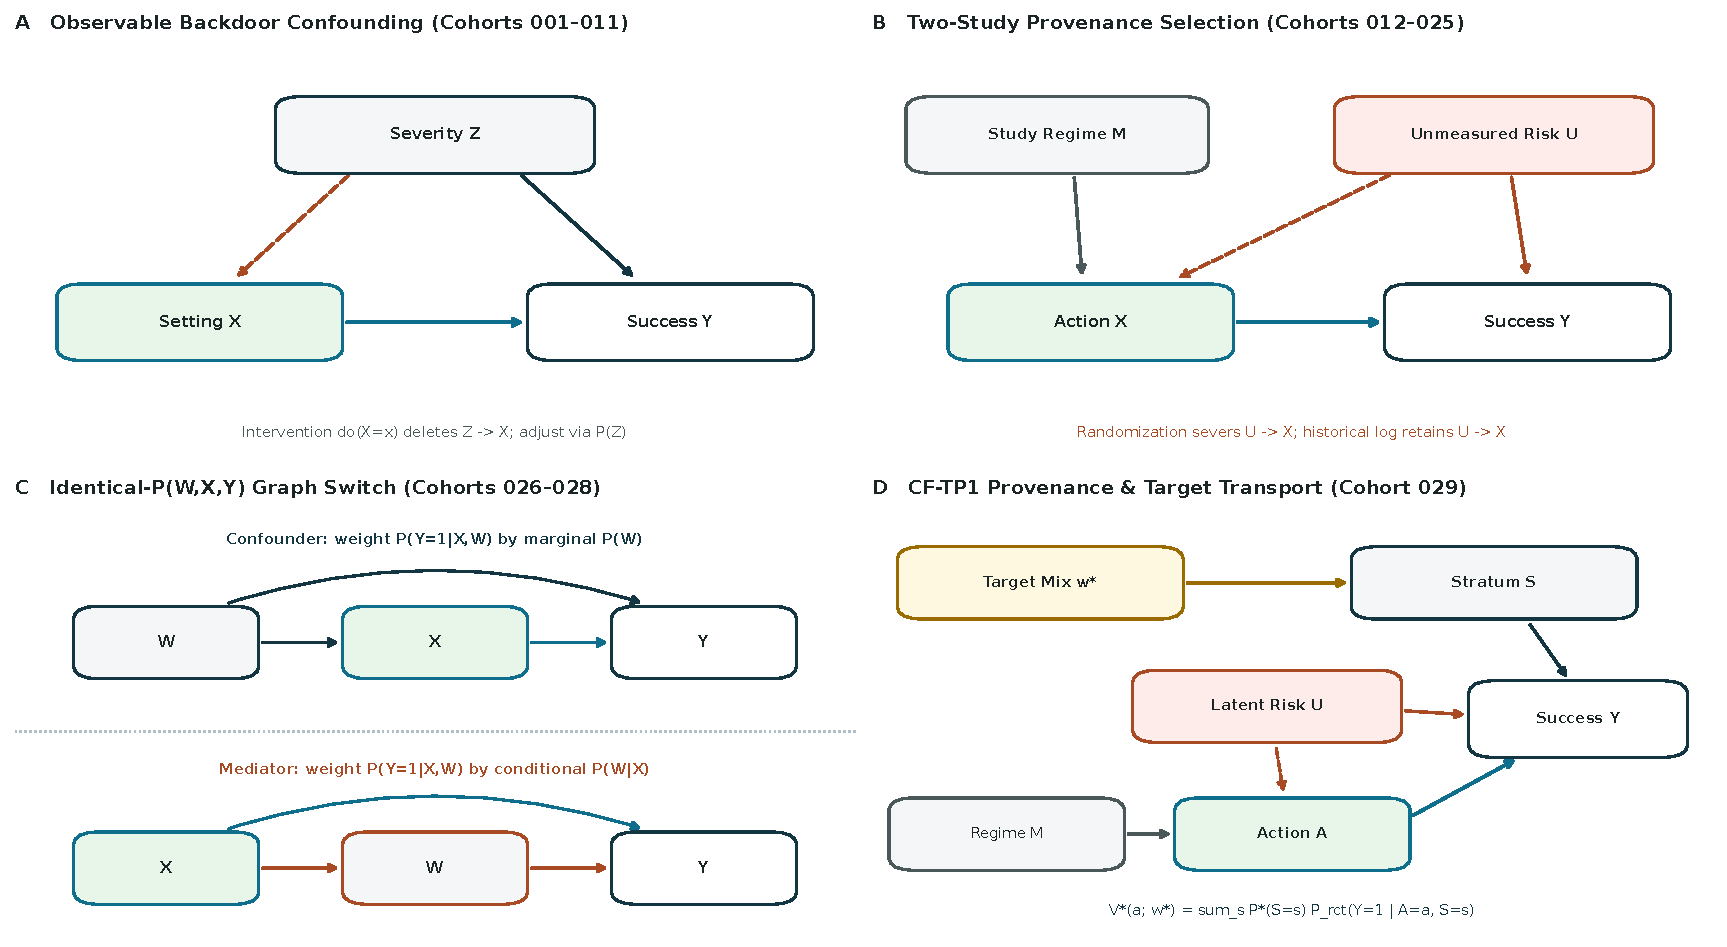
\includegraphics[width=\textwidth]{figures/fig08_structural_causal_diagrams.pdf}
  \caption{The four structural causal graph architectures investigated across Project CausalFade: (A) Observable backdoor confounding $Z\to X,Y$ (Cohorts~001--011); (B) Two-study randomized vs.\ unmeasured-confounder historical evidence (Cohorts~012--025); (C) Observationally equivalent confounder vs.\ mediator structures on identical $P(W,X,Y)$ tables (Cohorts~026--028); and (D) Selection diagram for target-population causal transport under stratum-mix shift (\texttt{CF-TP1}, Cohort~029).}
  \label{fig:scms}
\end{figure}

% =============================================================================
\section{Structural Causal Models, DAGs, and Conditional Independence}

\subsection{Intuitive Explanation}
Ordinary probability distributions describe \emph{which variables move together}, not \emph{which variable pushes which}. If severe machine wear ($Z=1$) prompts human operators to turn on an emergency cooling mode ($X=1$) and also causes frequent breakdowns ($Y=0$), then $X=1$ and $Y=0$ co-occur in historical logs even when cooling actually \emph{helps} every machine. A \textbf{Structural Causal Model (SCM)} writes down the directional data-generating mechanisms of the world as asymmetric assignments ($Y \leftarrow f_Y(X,Z,U_Y)$, read as ``nature computes $Y$ from $X$, $Z$, and exogenous noise $U_Y$''), while a \textbf{Directed Acyclic Graph (DAG)} draws those direct functional dependencies as arrows without feedback loops.

\subsection{Formal Scientific Definition and Mathematical Formulation}
\begin{definition}[Structural Causal Model and Induced Observational Law \citep{pearl2009causality}]
A Markovian Structural Causal Model is a tuple $\mathcal{M} = \langle \mathcal{U}, \mathcal{V}, \mathcal{F}, \Prob(\mathcal{U}) \rangle$, where $\mathcal{V} = \{V_1,\dots,V_m\}$ are endogenous variables, $\mathcal{U} = \{U_1,\dots,U_m\}$ are mutually independent exogenous background variables governed by product measure $\Prob(\mathcal{U}) = \prod_{j=1}^m \Prob(U_j)$, and $\mathcal{F} = \{f_1,\dots,f_m\}$ is a collection of structural equations
\begin{equation}
  V_j \coloneqq f_j(\mathrm{pa}_j, U_j), \qquad j = 1,\dots,m,
\end{equation}
whose parent sets $\mathrm{pa}_j \subseteq \mathcal{V}\setminus\{V_j\}$ form a Directed Acyclic Graph $\mathcal{G} = (\mathcal{V}, \mathcal{E})$ with directed edges $W \to V_j$ for each $W \in \mathrm{pa}_j$. Every Markovian SCM induces a unique joint observational distribution factoring along $\mathcal{G}$:
\begin{equation}
  \Prob_{\mathcal{M}}(v_1,\dots,v_m) = \prod_{j=1}^m \Prob(v_j \mid \mathrm{pa}_j).
  \label{eq:markov_factorization}
\end{equation}
\end{definition}

Conditional independence $A \Ind B \mid C$ means $\Prob(A,B\mid C) = \Prob(A\mid C)\Prob(B\mid C)$. In a DAG $\mathcal{G}$, Pearl's graphical criterion of \textbf{$d$-separation} characterizes every structural conditional independence implied by~\eqref{eq:markov_factorization}: a set of nodes $C$ blocks a path between $A$ and $B$ iff the path contains either a chain $i \to m \to j$ or fork $i \leftarrow m \to j$ with $m \in C$, or a collider $i \to c \leftarrow j$ such that neither $c$ nor any descendant of $c$ lies in $C$.

\subsection{Application, Evidence, and Limitations in CausalFade}
Figure~\ref{fig:scms} displays the four specific DAG architectures instantiated across CausalFade's 29 cohorts. In Cohorts~001--011 (Figure~\ref{fig:scms}A), $\mathcal{V} = \{Z, X, Y\}$ with fork $Z \leftarrow$ splitting into $Z \to X$ and $Z \to Y$ alongside causal edge $X \to Y$; conditioning on $Z$ blocks the noncausal backdoor path $X \leftarrow Z \to Y$. Conversely, in Cohorts~026--028 (Figure~\ref{fig:scms}C), when $W$ is a \emph{mediator} on the directed path $X \to W \to Y$, conditioning on $W$ blocks part of the desired causal effect rather than removing confounding! Empirically, Cohort~001 showed \texttt{Qwen2.5-3B F16} outputting \texttt{"adjustment\_set": ["X"]} ($0/64$ valid adjustment sets), conditioning on the treatment variable itself rather than the confounder $Z$, while Cohort~028 showed \texttt{Qwen2.5-7B F16} and \texttt{Llama-3.1-8B F16} choosing between \texttt{marginal} and \texttt{conditional} weighting at near-chance rates ($68/128$ and $60/128$) despite explicit DAG descriptions in the prompt. \emph{Limitation:} DAGs encode qualitative conditional independence and causal ancestry; as Cohorts~026--028 proved via exact rational tables, two distinct DAGs ($W\to X,Y$ vs.\ $X\to W\to Y$) can generate the \emph{exact same} observational joint table $\Prob(W,X,Y)$, meaning observational numbers alone can never identify the graph without external structural or temporal knowledge.

% =============================================================================
\section{Observational vs.\ Interventional Distributions and Pearl's \texorpdfstring{$\doop$}{do}-Operator}

\subsection{Intuitive and Formal Explanation}
Observing $X=x$ (\emph{seeing}) updates our beliefs about upstream causes of $X$: seeing an operator activate emergency cooling tells us the machine was probably already overheating. Intervening $\doop(X=x)$ (\emph{doing}) surgically overrides the operator's decision mechanism, forcing $X \coloneqq x$ for every unit regardless of initial state. Graphically, $\doop(X=x)$ deletes all incoming arrows into $X$ while leaving every other structural equation untouched.

\subsection{Mathematical Formulation: Truncated Factorization, ATE, CATE, and Simpson's Reversal}
In SCM $\mathcal{M}$, replacing $X \coloneqq f_X(\mathrm{pa}_X, U_X)$ with constant assignment $X \coloneqq x$ defines the mutilated submodel $\mathcal{M}_x$, whose interventional distribution obeys the \textbf{truncated factorization}:
\begin{equation}
  \Prob(v_1,\dots,v_m \mid \doop(X=x)) = \mathbb{I}(v_X = x) \prod_{V_j \neq X} \Prob(v_j \mid \mathrm{pa}_j).
  \label{eq:truncated_factorization}
\end{equation}
When covariate set $Z$ satisfies the \textbf{backdoor criterion} relative to $(X,Y)$---meaning no node in $Z$ is a descendant of $X$ and $Z$ blocks every path between $X$ and $Y$ containing an arrow into $X$---summing~\eqref{eq:truncated_factorization} yields Pearl's \textbf{backdoor adjustment formula}:
\begin{equation}
  \Prob(Y=1 \mid \doop(X=x)) = \sum_{z} \Prob(Y=1 \mid X=x, Z=z)\,\Prob(Z=z),
  \label{eq:backdoor}
\end{equation}
provided positivity $\Prob(X=x\mid Z=z) > 0$ holds for all strata with $\Prob(Z=z)>0$. By contrast, the naive observational conditional probability weights those exact same stratum success rates by \emph{treatment-conditioned} covariate shares:
\begin{equation}
  \Prob(Y=1 \mid X=x) = \sum_{z} \Prob(Y=1 \mid X=x, Z=z)\,\Prob(Z=z \mid X=x).
  \label{eq:obs_expansion}
\end{equation}
Comparing~\eqref{eq:backdoor} and~\eqref{eq:obs_expansion} makes confounding bias algebraically transparent. Define the stratum-specific \textbf{Conditional Average Treatment Effect ($\CATE$)}, population \textbf{Average Treatment Effect ($\ATE$)}, and naive \textbf{Observational Risk Difference ($\RD_{\mathrm{obs}}$)} for binary $Y \in \{0,1\}$:
\begin{align}
  \tau(z) &= \Prob(Y=1\mid X=1,Z=z) - \Prob(Y=1\mid X=0,Z=z) \nonumber\\
          &= \E[Y \mid \doop(X=1), Z=z] - \E[Y \mid \doop(X=0), Z=z], \label{eq:cate}\\
  \ATE &= \E[Y \mid \doop(X=1)] - \E[Y \mid \doop(X=0)] = \sum_{z} \tau(z)\,\Prob(Z=z), \label{eq:ate}\\
  \RD_{\mathrm{obs}} &= \Prob(Y=1 \mid X=1) - \Prob(Y=1 \mid X=0). \label{eq:rd_obs}
\end{align}
When confounding shifts $\Prob(Z=1\mid X=1)$ far away from $\Prob(Z=1\mid X=0)$, $\ATE$ and $\RD_{\mathrm{obs}}$ can have \emph{strictly opposite signs} ($\ATE \cdot \RD_{\mathrm{obs}} < 0$), known as \textbf{Simpson's reversal}.

\begin{workedexample}[Actual CausalFade Cohort~001 World \texttt{world-0000}, Task \texttt{cb2060af78e213308f0e}]
In \texttt{results/design\_validation/public\_tasks.jsonl} (line~1, reused in Cohort~001), $\Prob(Z=0)=\Prob(Z=1)=0.5$, and the exact stratum quantities are:
\begin{itemize}
  \item $Z=0$ (mild): $\Prob(Y=1\mid X=0,Z=0)=0.833549$ (cell mass $0.442746$), $\Prob(Y=1\mid X=1,Z=0)=0.738055$ (cell mass $0.057254$). Thus $\tau(0) = 0.738055 - 0.833549 = -0.095494$ ($-9.55\pp$).
  \item $Z=1$ (severe): $\Prob(Y=1\mid X=0,Z=1)=0.261945$ (cell mass $0.057254$), $\Prob(Y=1\mid X=1,Z=1)=0.166451$ (cell mass $0.442746$). Thus $\tau(1) = 0.166451 - 0.261945 = -0.095494$ ($-9.55\pp$).
\end{itemize}
Here both strata suffer a $-9.55\pp$ causal harm from activating $X$, so $\ATE = 0.5(-0.095494) + 0.5(-0.095494) = -0.095494 < 0$ (optimal action: \texttt{activate=0}). Because operators disproportionately activate $X$ when $Z=1$ ($\Prob(Z=1\mid X=1) = 0.8855$), the naive observational difference is even more negative ($\RD_{\mathrm{obs}} = 0.2319 - 0.7681 = -0.5362$), forming an \emph{aligned-negative} cell ($T=0, S=0$). Flipping the operator selection propensity in line~3 (\texttt{28a407789b6fcdab736f}) so operators activate $X$ mainly when $Z=0$ reverses $\RD_{\mathrm{obs}}$ to $+0.3609 > 0$ while keeping $\ATE = -0.095494 < 0$ unchanged, creating a \emph{conflict} cell ($T=0, S=1$)!
\end{workedexample}

\begin{pedagogicalexample}[Constructed Teaching Example: Confounder vs.\ Mediator on Identical Numbers]
\emph{(Constructed with simple round numbers for classroom clarity; see Chapter~11 for actual Cohort~027 six-decimal tables.)} Suppose an observational dataset of $100$ machines has exact joint counts:
\begin{itemize}
  \item Among $X=0$ ($50$ units): $10$ have $W=0$ ($8$ succeed, $80\%$) and $40$ have $W=1$ ($16$ succeed, $40\%$). Overall $X=0$ success is $(8+16)/50 = 48\%$.
  \item Among $X=1$ ($50$ units): $40$ have $W=0$ ($28$ succeed, $70\%$) and $10$ have $W=1$ ($3$ succeed, $30\%$). Overall $X=1$ success is $(28+3)/50 = 62\%$.
\end{itemize}
Notice that overall marginal prevalence is $\Prob(W=0) = (10+40)/100 = 0.50$ and $\Prob(W=1) = 0.50$.
\begin{enumerate}
  \item \textbf{Case A ($W$ is a pre-treatment confounder, $W \to X, Y$):} Intervening on $X$ does \emph{not} change $W$, so we weight by marginal $\Prob(W)=(0.5, 0.5)$: $\Prob(Y=1\mid \doop(X=0)) = 0.5(80\%) + 0.5(40\%) = 60\%$, while $\Prob(Y=1\mid \doop(X=1)) = 0.5(70\%) + 0.5(30\%) = 50\%$. Activating $X$ \emph{lowers} success by $-10\pp$ (\textbf{choose $X=0$}).
  \item \textbf{Case B ($W$ is a post-treatment mediator, $X \to W \to Y$, no unmeasured confounding):} Activating $X$ \emph{causes} $W=0$ to rise from $20\%$ to $80\%$, so the total interventional effect uses $\Prob(W\mid X=x)$: $\Prob(Y=1\mid \doop(X=0)) = \Prob(Y=1\mid X=0) = 48\%$, while $\Prob(Y=1\mid \doop(X=1)) = \Prob(Y=1\mid X=1) = 62\%$. Activating $X$ \emph{raises} success by $+14\pp$ (\textbf{choose $X=1$}).
\end{enumerate}
Same table, opposite optimal interventions! This exact mathematical duality drove Cohorts~026--028.
\end{pedagogicalexample}

% =============================================================================
\section{Randomized Evidence, Target-Population Transport, and Pairwise Fidelity}

\subsection{Intuitive Explanation}
Why did CausalFade evolve from single-table backdoor adjustment (Cohorts~001--011) and two-study aggregate comparisons (Cohorts~012--025) to \textbf{target-population transportability} in Cohort~029 (\texttt{CF-TP1})? In two-study aggregate tasks, once a model picks the randomized study, all that remains is comparing two printed numbers (\texttt{off 54.11\%, on 45.89\%})---a trivial single-inequality check easily mimicked by magnitude heuristics. Real-world policy decisions are harder in a structurally fundamental way:
\begin{enumerate}
  \item We have \textbf{two studies}: a historical study corrupted by unmeasured operator selection risk $U$, and a randomized trial where random assignment severs $U \to A$.
  \item Treatment helps one pre-treatment subgroup (say, \texttt{Blue}) and hurts another (\texttt{Amber})---known as \emph{qualitative CATE heterogeneity}.
  \item The \textbf{target population} where we must deploy the policy has its own subgroup composition $(w^*, 1-w^*)$, which differs from historical enrollment!
\end{enumerate}

\subsection{Formal Definition and Mathematical Formulation}
Let $S \in \{0,1\}$ denote a pre-treatment baseline group (\texttt{Amber} $=0$, \texttt{Blue} $=1$), $U \in \{0,1\}$ an unmeasured risk factor, $M \in \{\mathrm{rct}, \mathrm{hist}\}$ the study regime, $A \in \{0,1\}$ the treatment action, and $Y \in \{0,1\}$ success (Figure~\ref{fig:scms}D).
\begin{itemize}
  \item Under the \textbf{randomized study} ($M=\mathrm{rct}$), $A \Ind U \mid S$, so observed group-specific rates identify true stratum potential-outcome expectations:
  \begin{equation}
    \mu_{\mathrm{rct}}(s, a) = \Prob(Y=1 \mid M=\mathrm{rct}, S=s, A=a) = \E[Y(a) \mid S=s].
  \end{equation}
  \item Under the \textbf{historical study} ($M=\mathrm{hist}$), operators choose $A$ partly based on unmeasured risk $U$ ($U \to A$ and $U \to Y$), so $\mu_{\mathrm{hist}}(s, a) = \Prob(Y=1 \mid M=\mathrm{hist}, S=s, A=a) \neq \E[Y(a) \mid S=s]$ even within stratum $S=s$!
  \item Under \textbf{stratum transportability} \citep{pearl2014external,westreich2017transportability}---conditional causal effects $\E[Y(a)\mid S=s]$ carry over unchanged to a target population $\Pi^*$ with known stratum share $w^* = \Prob^*(S=0) \in (0,1)$---the target interventional value of action $a$ and standardized causal effect $\tau^*(w^*)$ are:
  \begin{align}
    V^*(a; w^*) &= \Prob^*(Y=1 \mid \doop(A=a)) = w^*\,\mu_{\mathrm{rct}}(0,a) + (1-w^*)\,\mu_{\mathrm{rct}}(1,a), \label{eq:transport_val}\\
    \tau^*(w^*) &= V^*(1; w^*) - V^*(0; w^*) = w^*\,\delta_{\mathrm{rct}}(0) + (1-w^*)\,\delta_{\mathrm{rct}}(1), \label{eq:transport_ate}
  \end{align}
  where $\delta_{\mathrm{rct}}(s) = \mu_{\mathrm{rct}}(s,1) - \mu_{\mathrm{rct}}(s,0)$. Whenever $\delta_{\mathrm{rct}}(0)$ and $\delta_{\mathrm{rct}}(1)$ have opposite signs, $\tau^*(w^*)$ is an affine function of $w^*$ that crosses zero at the interior threshold
  \begin{equation}
    w_{\mathrm{crit}} = \frac{-\delta_{\mathrm{rct}}(1)}{\delta_{\mathrm{rct}}(0) - \delta_{\mathrm{rct}}(1)} \in (0,1).
    \label{eq:w_crit}
  \end{equation}
\end{itemize}

Consequently, evaluating the \emph{exact same two study tables} at two target population mixes $w_0 < w_{\mathrm{crit}} < w_1$ forces a causally competent decision-maker to \textbf{reverse} its optimal action $a^*(w) = \mathbb{I}(\tau^*(w) > 0)$! Conversely, if two target mixes lie on the same side of $w_{\mathrm{crit}}$ (or if both strata share the same sign in one of the balanced sign-matrix strata), the optimal decision must be \textbf{retained} (invariance). Figure~\ref{fig:transport_f096} illustrates this exact geometry on Cohort~029's archived Family~\texttt{096}.

\begin{figure}[htbp]
  \centering
  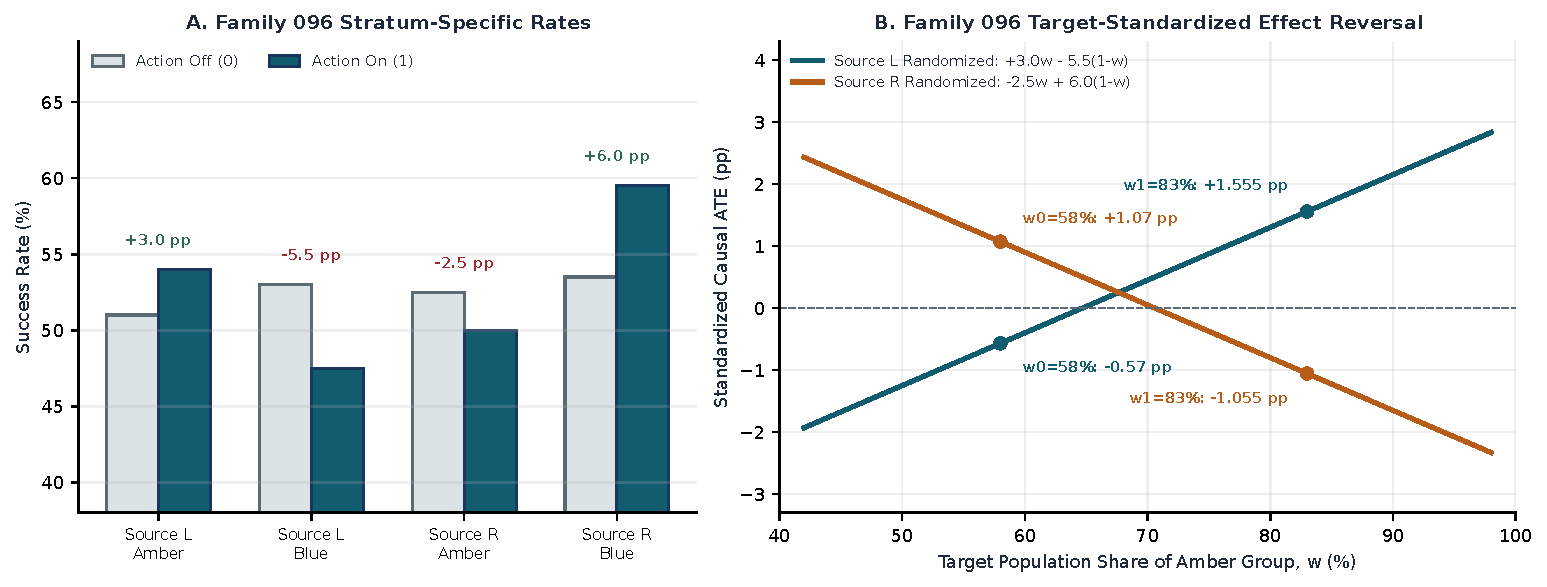
\includegraphics[width=\textwidth]{figures/fig10_target_population_transport.pdf}
  \caption{Target-population causal transport in archived \texttt{CF-TP1} Family~\texttt{096} (\texttt{experiments/cohort\_029/freeze/fixture/worlds.jsonl}): (A) Stratum-specific off/on percentages in Source~L and Source~R; (B) Standardized causal effect lines $\tau_k(w)$ reversing sign between Mix~0 ($w_0=58\%$) and Mix~1 ($w_1=83\%$).}
  \label{fig:transport_f096}
\end{figure}

\subsection{Decision Reversal, Retention, and Pairwise Fidelity}
Consider any pair of minimally contrasted tasks $(x_0, x_1)$ with gold binary actions $(g_0, g_1) \in \{0,1\}^2$ and model predictions $(\hat{a}_0, \hat{a}_1) \in \{0,1\}^2$. Let $I_m = \mathbb{I}(\hat{a}_m = g_m)$ be single-item correctness on member $m \in \{0,1\}$.
\begin{itemize}
  \item \textbf{Single-item accuracy} $\frac{1}{2}(I_0 + I_1)$ awards $50\%$ credit on every reversal pair ($g_0 \neq g_1$) to a degenerate constant policy ($\hat{a}_0 = \hat{a}_1 = 1$), because any constant answer matches whichever member happens to have gold label $1$!
  \item \textbf{Pairwise bundle fidelity} \citep{gardner2020contrast} scores $1$ iff \emph{both} members of the pair are answered correctly:
  \begin{equation}
    F_{\mathrm{pair}}(x_0, x_1) = I_0 \cdot I_1 = \mathbb{I}(\hat{a}_0 = g_0 \;\wedge\; \hat{a}_1 = g_1).
    \label{eq:pair_fidelity}
  \end{equation}
\end{itemize}
On a \textbf{switch pair} ($g_0 \neq g_1$), $F_{\mathrm{pair}} = 1$ requires both switching ($\hat{a}_0 \neq \hat{a}_1$) \emph{and} getting the direction right ($\hat{a}_0 = g_0$); any constant policy ($\hat{a}_0 = \hat{a}_1$) receives $F_{\mathrm{pair}} = 0$! Simultaneously, including an equal number of \textbf{invariant pairs} ($g_0 = g_1$) prevents an adversarial heuristic that blindly alternates answers across pairs from gaming switch pairs, because blind alternation scores $F_{\mathrm{pair}} = 0$ on invariant pairs (Figure~\ref{fig:reversal_retention}).

\begin{figure}[htbp]
  \centering
  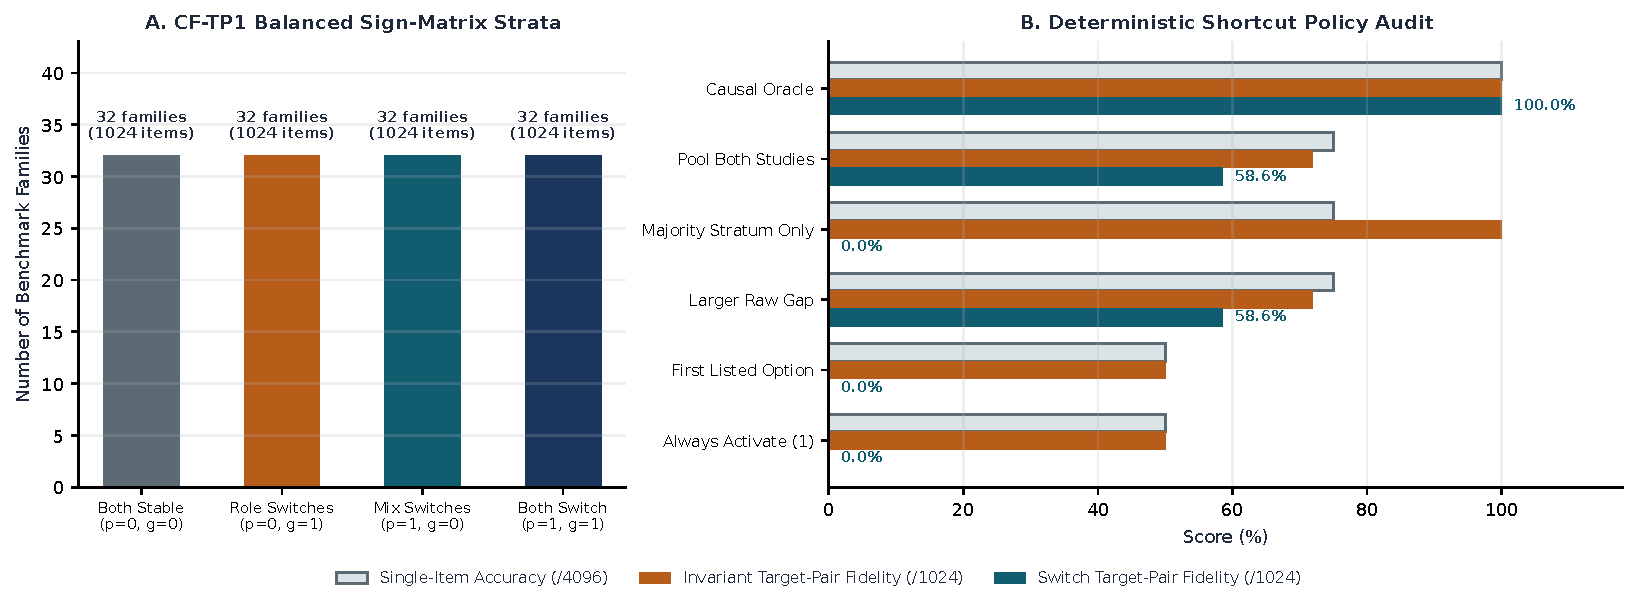
\includegraphics[width=\textwidth]{figures/fig11_decision_reversal_retention.pdf}
  \caption{Balanced sign-matrix design and shortcut policy audit in \texttt{CF-TP1}: (A) Four $32$-family sign-matrix strata $(p,g)\in\{0,1\}^2$ balancing reversal and invariance across target-mix and source-role axes; (B) Why single-item accuracy ($50\%$) and invariant pairs ($50\%$) fail to expose constant-activation or option-order policies, whereas switch-pair fidelity drives constant policies to $0\%$.}
  \label{fig:reversal_retention}
\end{figure}

% =============================================================================
\section{Psychometric Decompositions: C/A/B Trees and Signal Detection Theory}

\subsection{The C/A/B Multinomial Processing Tree---and Why It Failed}
Adapted from \citet{jacoby1991process} and \citet{gawronski2017cni} during \texttt{design\_validation} (\texttt{causalfade/cab\_tree.py}), the 3-parameter Causal/Associative/Bias ($C/A/B$) tree models the probability of choosing \texttt{activate=1} given causal cue $T \in \{0,1\}$ and associative cue $S \in \{0,1\}$ as:
\begin{equation}
  \Prob(\text{act}=1 \mid T, S) = p_{TS} = C \cdot T + (1 - C)\bigl[A \cdot S + (1 - A) B\bigr], \qquad C, A, B \in [0,1].
  \label{eq:cab_tree}
\end{equation}
Expanding~\eqref{eq:cab_tree} over $(T,S) \in \{0,1\}^2$ yields four linear equations in $(w_C, w_A, w_B) = (C, (1-C)A, (1-C)(1-A)B)$:
\begin{align}
  p_{11} &= C + (1-C)A + (1-C)(1-A)B, & p_{10} &= C + (1-C)(1-A)B, \nonumber\\
  p_{01} &= (1-C)A + (1-C)(1-A)B,     & p_{00} &= (1-C)(1-A)B. \label{eq:cab_cells}
\end{align}
Because four binomial cell probabilities $(p_{11}, p_{10}, p_{01}, p_{00})$ are fitted by three parameters,~\eqref{eq:cab_cells} imposes an exact \textbf{zero-interaction additivity constraint}:
\begin{equation}
  \mathcal{I}_{\mathrm{tree}} \coloneqq p_{11} - p_{10} - p_{01} + p_{00} = 0.
  \label{eq:cab_additivity}
\end{equation}
Two fatal limitations surfaced immediately in CausalFade (Figure~\ref{fig:cab_recovery}):
\begin{enumerate}
  \item \textbf{Observational equivalence to continuous cue integration (\texttt{design\_validation}):} Any symmetric additive logistic model $\Prob(\text{act}=1\mid T,S) = \sigma\bigl(\beta_T(2T-1) + \beta_S(2S-1)\bigr)$ with zero intercept satisfies $p_{00} + p_{11} = 1$ and $p_{10} + p_{01} = 1$, which algebraically implies $p_{11} - p_{10} - p_{01} + p_{00} = (1-p_{00}) - p_{10} - (1-p_{10}) + p_{00} = 0$! Hence a 4-cell table can \emph{never} distinguish sequential discrete gating ($C \to A \to B$) from simultaneous weighted evidence summation ($p_{\text{boot}} = 0.433$).
  \item \textbf{Empirical violation of additivity (Cohort~005):} On \texttt{Qwen2.5-3B F16}, observed cell probabilities yielded $\widehat{\mathcal{I}}_{\mathrm{tree}} = -0.4375$ ($-43.75\pp$, 95\% CI $[-68.75, -18.75]\pp$), decisively falsifying cross-cell parameter invariance.
\end{enumerate}

\begin{figure}[htbp]
  \centering
  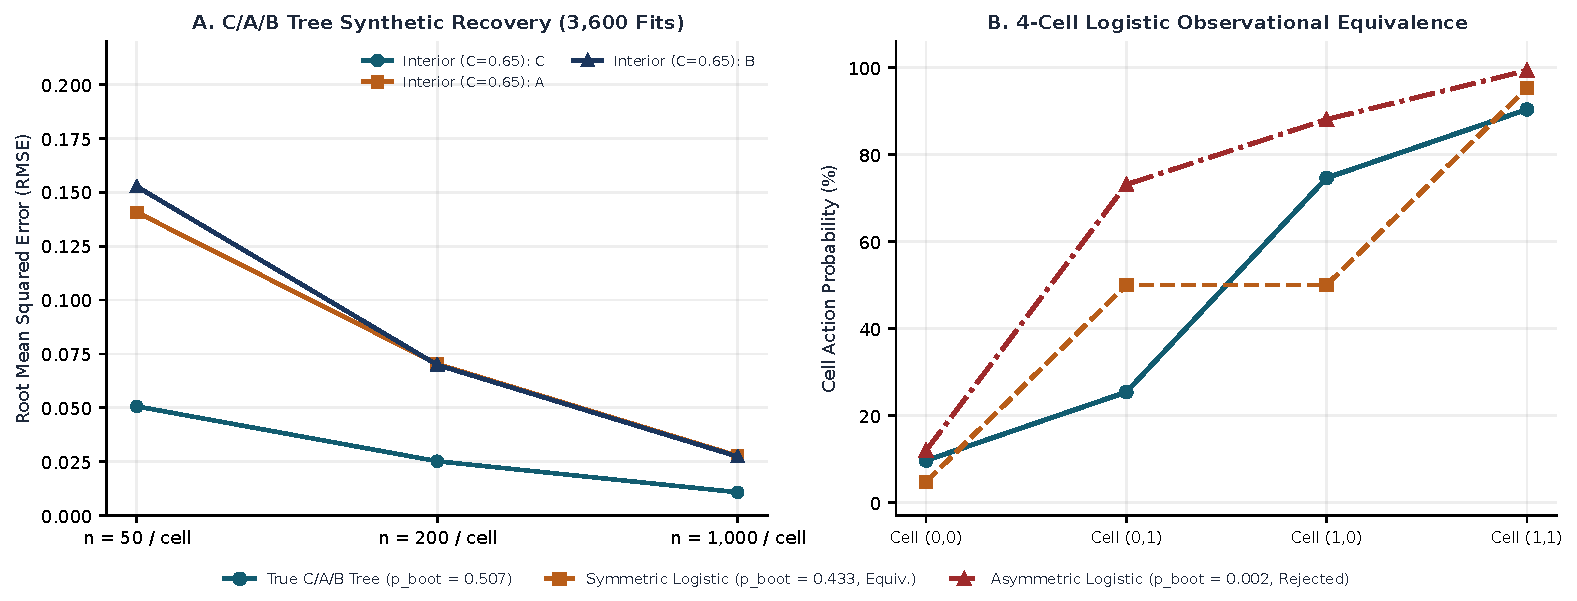
\includegraphics[width=\textwidth]{figures/fig18_synthetic_cab_recovery.pdf}
  \caption{Pre-LLM synthetic validation of the $C/A/B$ processing tree (\texttt{results/design\_validation/parameter\_recovery.json}, $3{,}600$ EM fits): (A) RMSE across cell sizes $n\in\{50,200,1000\}$ showing inflation of conditional parameter error when $C$ is high or $n$ is small; (B) Exact observational equivalence between the discrete $C/A/B$ tree and symmetric logistic cue integration ($p_{\text{boot}}=0.433$).}
  \label{fig:cab_recovery}
\end{figure}

\subsection{Signal Detection Theory (\texorpdfstring{$d'$}{d'} and Criterion \texorpdfstring{$c$}{c})}
To summarize binary sensitivity and directional response bias without assuming sequential latent branches, Cohort~024 adopted \textbf{Signal Detection Theory} \citep{jones2016cue}. Defining the hit rate $H = \Prob(\hat{a}=1 \mid g=1)$ and false-alarm rate $F = \Prob(\hat{a}=1 \mid g=0)$ (with log-linear / half-count boundary smoothing $(k+0.5)/(n+1)$ so $\Phi^{-1}(\cdot)$ remains finite when $k=0$ or $k=n$), sensitivity $d'$ and decision criterion $c$ are:
\begin{equation}
  d' = \Phi^{-1}(H) - \Phi^{-1}(F), \qquad c = -\frac{1}{2}\bigl[\Phi^{-1}(H) + \Phi^{-1}(F)\bigr],
  \label{eq:sdt}
\end{equation}
where $\Phi^{-1}$ is the standard normal probit function. Here $d'=0$ indicates zero discrimination between beneficial ($g=1$) and harmful ($g=0$) interventions, $c < 0$ indicates liberal \texttt{activate=1} bias, and $c > 0$ indicates conservative \texttt{decline} (\texttt{activate=0}) bias.

% =============================================================================
\section{Floating-Point Precision and GGUF Block-Affine Quantization}

\subsection{Intuitive and Formal Explanation}
In unquantized half-precision (\texttt{F16}, IEEE~754 \texttt{binary16}), each neural network weight uses $16$ bits ($1$ sign bit, $5$ exponent bits, $10$ mantissa bits), representing values across $\sim 10^{-5}$ to $65{,}504$ with roughly $3.3$ significant decimal digits. \textbf{Post-Training Quantization (PTQ)} in the \texttt{llama.cpp} \texttt{GGUF} ecosystem partitions weight rows into small contiguous blocks (e.g., $32$ weights in \texttt{Q8\_0}, or $256$-weight ``super-blocks'' subdivided into $16$--$32$-weight sub-blocks in K-quants \texttt{Q6\_K}, \texttt{Q5\_K\_M}, \texttt{Q4\_K\_M}, \texttt{Q3\_K\_M}, \texttt{Q2\_K}) and stores low-bit integers alongside shared floating-point block scales and offsets.

\subsection{Mathematical Formulation and Bits-Per-Weight (\texorpdfstring{$\BPW$}{BPW})}
For a block $\mathbf{w} \in \mathbb{R}^B$ under symmetric $b$-bit quantization (such as \texttt{Q8\_0}, $B=32$, $b=8$), quantization and dequantization compute:
\begin{equation}
  s = \frac{\max_i |w_i|}{2^{b-1}-1}, \qquad q_i = \operatorname{round}\!\left(\frac{w_i}{s}\right) \in \{-127,\dots,127\}, \qquad \widehat{w}_i = s \cdot q_i.
\end{equation}
In asymmetric hierarchical K-quants (e.g., \texttt{Q4\_K\_M}, \texttt{Q2\_K}), a 256-weight super-block stores FP16 super-scales $(d, d_{\min})$, quantized 6-bit or 4-bit sub-block scales $(s_m, k_m)$, and $b$-bit integer weights $q_{m,j} \in \{0,\dots,2^b-1\}$, reconstructing
\begin{equation}
  \widehat{w}_{m,j} = (d \cdot s_m)\, q_{m,j} - (d_{\min} \cdot k_m), \qquad \text{with reconstruction error } \varepsilon_{m,j} = \widehat{w}_{m,j} - w_{m,j}.
  \label{eq:kquant}
\end{equation}
Because scale metadata and mixed-precision attention/output tensors (\texttt{\_M} suffix promotes sensitive tensors such as \texttt{attn\_v} or \texttt{ffn\_down} to higher bit-widths) add overhead beyond $b$ bits, effective compression is measured in \textbf{bits per weight ($\BPW$)}:
\begin{equation}
  \BPW = \frac{8 \times \text{TensorBytes}_{\mathrm{quantized}}}{N_{\mathrm{parameters}}}.
\end{equation}
Across CausalFade's inventory (Chapter~4), \texttt{F16} sits at $16.00\;\BPW$, \texttt{Q8\_0} at $\approx 8.50\;\BPW$, \texttt{Q6\_K} at $\approx 6.56\;\BPW$, \texttt{Q5\_K\_M} at $\approx 5.69\;\BPW$, \texttt{Q4\_K\_M} at $\approx 4.85\;\BPW$, \texttt{Q3\_K\_M} at $\approx 3.91\;\BPW$, and \texttt{Q2\_K} at $\approx 2.96\;\BPW$.

% =============================================================================
\section{Construct Validity, Shortcuts, Matched Controls, and Clustered Inference}

\subsection{Benchmark Shortcuts and Matched Experimental Controls}
A benchmark possesses \textbf{construct validity} iff high scores can be achieved \emph{only} by exercising the target cognitive or mathematical capability, and low scores reflect genuine deficits in that capability rather than extraneous formatting or arithmetic bottlenecks. Let $\mathcal{H}_{\mathrm{shortcut}}$ denote a class of deterministic surface policies that inspect printed numbers, token positions, or study order \emph{without} using causal identification rules. If there exists $h \in \mathcal{H}_{\mathrm{shortcut}}$ with high benchmark score, any LLM matching $h$ will appear ``causally competent'' for noncausal reasons \citep{mccoy2019right}. Conversely, if an LLM fails a causal task solely because it cannot multiply two percentages and add them, attributing that failure to ``lack of causal understanding'' commits the inverse construct-validity error. CausalFade resolved both sides of this trap by combining:
\begin{enumerate}
  \item \textbf{Pre-execution shortcut audits:} Proving over $162$ deterministic noncausal policies in Cohort~029 (\texttt{policy\_audit.json}) that no rule ignoring source provenance or target composition exceeds structural chance ceilings on pairwise fidelity; and
  \item \textbf{Matched noncausal controls:} Pairing every causal task with an isomorphic noncausal scorecard task over the \emph{exact same numbers, weights, options, and JSON output schema}, isolating causal identification overhead via the paired within-family difference $D_i = Y_{i,\mathrm{causal}} - Y_{i,\mathrm{control}}$.
\end{enumerate}

\subsection{Clustered Variance and Dual Parametric/Bounded Confidence Intervals}
Because each synthetic world family $i \in \{1,\dots,N\}$ generates multiple correlated prompt items (e.g., $32$ prompts and $8$ transfer target pairs per family in Cohort~029), treating individual prompts as independent Bernoulli trials ($n=4{,}096$) severely underestimates standard errors (pseudo-replication). The statistically valid unit of randomization and independence is the \textbf{world family cluster} $i$.

In Cohort~029's stratified design of $H=8$ equal strata of $m_h = 16$ independent families ($N = \sum_{h=1}^8 m_h = 128$), let $D_{hi} \in [-1, 1]$ denote the family-level causal-minus-arithmetic difference in transfer target-pair fidelity for family $i$ in stratum $h$, with stratum sample mean $\bar{D}_h = \frac{1}{m_h}\sum_{i=1}^{m_h} D_{hi}$ and stratum sample variance $s_h^2 = \frac{1}{m_h-1}\sum_{i=1}^{m_h}(D_{hi}-\bar{D}_h)^2$. The stratified estimator, standard error, and Welch--Satterthwaite degrees of freedom \citep{welch1947generalization} are:
\begin{equation}
  \widehat{\Delta} = \frac{1}{H}\sum_{h=1}^H \bar{D}_h, \qquad
  \widehat{\mathrm{SE}}(\widehat{\Delta}) = \sqrt{\sum_{h=1}^H \frac{s_h^2}{H^2 m_h}}, \qquad
  \hat{\nu} = \frac{\left(\sum_{h=1}^H \frac{s_h^2}{H^2 m_h}\right)^2}{\sum_{h=1}^H \frac{(s_h^2 / (H^2 m_h))^2}{m_h - 1}},
  \label{eq:strat_welch}
\end{equation}
yielding the $95\%$ Welch $t$ interval $\widehat{\Delta} \pm t_{0.975, \hat{\nu}}\,\widehat{\mathrm{SE}}(\widehat{\Delta})$. Simultaneously, because $D_{hi} \in [-1, 1]$ has bounded range $b - a = 2$, Hoeffding's inequality \citep{hoeffding1963probability} guarantees finite-sample $(1-\alpha)$ coverage via the distribution-free radius
\begin{equation}
  r_{\mathrm{bounded}}(\alpha) = (b - a)\sqrt{\frac{\ln(2/\alpha)}{2 N}} = 2\sqrt{\frac{\ln(2/0.05)}{2 \times 128}} = 2\sqrt{\frac{\ln 40}{256}} \approx 0.240081 \;\;(24.01\pp),
  \label{eq:hoeffding_radius}
\end{equation}
producing Cohort~029's exact archived bounded interval $\widehat{\Delta} \pm 0.240081 = [-27.52\pp, +20.49\pp]$ (\texttt{primary.json}). Notice how equation~\eqref{eq:hoeffding_radius} reproduces the exact archived radius $-0.03515625 - (-0.27523695) = 0.24008070$ to eight decimal places!


% --- PART II: THE EXPERIMENTAL JOURNEY ---
\part{The Experimental Journey}
% =============================================================================
% Part II, Chapter 4: The Experimental Infrastructure
% =============================================================================
\chapter{The Experimental Infrastructure}\label{ch:infrastructure}

Empirical findings in LLM evaluation are only as trustworthy as the software, inference server, quantization pipeline, parser, and audit trail that produced them. Across CausalFade's twenty-nine-day history, infrastructure bugs and subtle execution defaults repeatedly masqueraded as cognitive discoveries---from Markdown code-fence mismatches in Cohort~001 to noncausal length-cap truncations in Cohort~024 and option-order coupling in Cohort~026. Equally important, every time such an artifact was uncovered, the researchers hardened the engineering stack rather than patching results by hand. This chapter documents the technical architecture of CausalFade and traces how its reproducibility safeguards evolved across four infrastructure generations (Figure~\ref{fig:infra_arch}).

\begin{figure}[htbp]
  \centering
  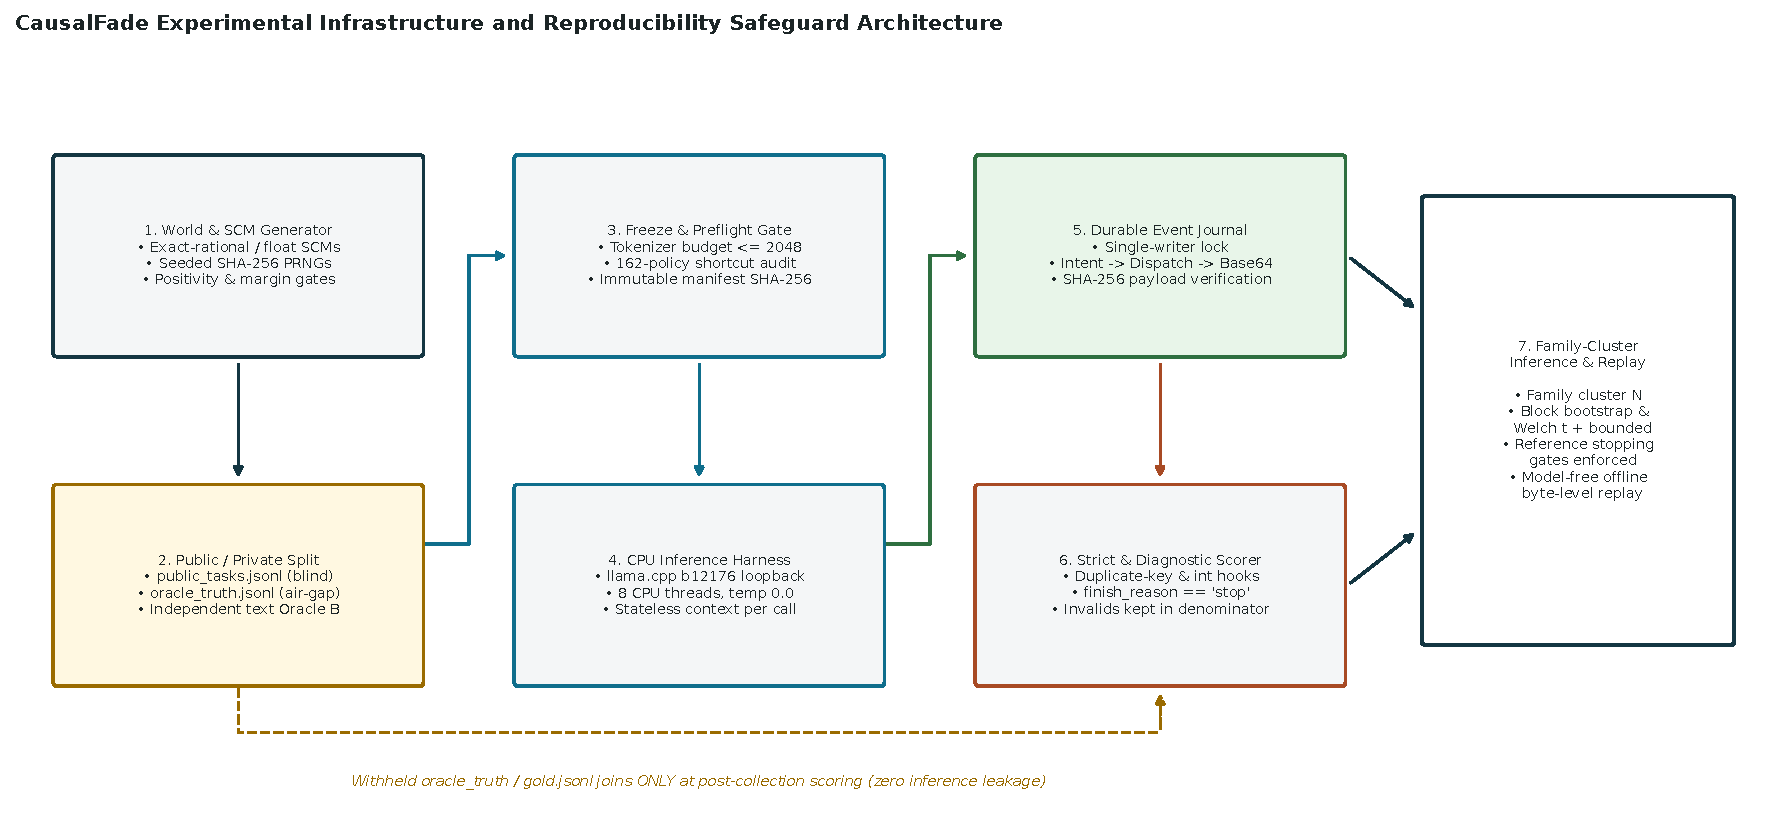
\includegraphics[width=\textwidth]{figures/fig07_infrastructure_architecture.pdf}
  \caption{End-to-end technical architecture of Project CausalFade, illustrating the strict air-gap between public prompt manifests and evaluator-only oracle truth, deterministic local \texttt{llama-server} execution, raw response journaling, strict vs.\ normalized parser layers, and family-clustered statistical scoring.}
  \label{fig:infra_arch}
\end{figure}

% =============================================================================
\section{Repository Organization and Four-Generation Evolution}

At snapshot commit \nolinkurl{b7371530caa62d6e43a8e83ef6db361f6640f63a}, the repository is organized into six functional layers:
\begin{enumerate}
  \item \textbf{Core Python Package (\texttt{causalfade/}):} Built during the initial validation phase (commits \texttt{6ab18d2}--\texttt{caf5b1d}), containing \texttt{scm.py} (binary backdoor SCM construction), \texttt{generate.py} (world family sampling and JSONL serialization), \texttt{cab\_tree.py} (multinomial processing tree EM solver and bootstrap deviance tests), \texttt{evaluate.py} (JSON response parsing and metric aggregation), and \texttt{runner.py} (local HTTP client against \texttt{llama-server}).
  \item \textbf{Operational Harnesses and Utilities (\texttt{tools/}):} Cohort-specific dataset builders, model preflight verifiers, RAM safety guards, deterministic calculator sandboxes (Cohort~028), and standalone audit scripts.
  \item \textbf{Pre-LLM Synthetic Validation (\texttt{results/design\_validation/}):} Frozen synthetic parameter-recovery artifacts ($3{,}600$ EM fits), logistic observational equivalence checks, and the initial $24$-family ($192$-prompt) testbed.
  \item \textbf{Experimental Cohort Archive (\texttt{experiments/cohort\_001/} through \texttt{cohort\_029/}):} Thirty self-contained cohort directories (including \texttt{cohort\_025\_1}) preserving input manifests, schedules, server logs, raw JSONL model responses, scored JSON summaries, and contemporaneous Markdown reports.
  \item \textbf{Governance and Audit Documentation (\texttt{EXPERIMENTS.md}, \texttt{DECISIONS.md}, \texttt{docs/}):} Chronological ledgers recording pre-execution contracts, hardware reuse manifests (\texttt{docs/SSD\_ASSET\_REUSE.md}), data contracts (\texttt{docs/DATA\_CONTRACT.md}), statistical analysis plans (\texttt{docs/STATISTICAL\_ANALYSIS\_PLAN.md}), and retrospective readiness audits.
  \item \textbf{Final Manuscript Package (\texttt{manuscript/}):} Self-contained publication source (\texttt{article.tex}, \texttt{supplement.tex}, \texttt{history.tex}), byte-level reconstruction scripts (\texttt{manuscript/scripts/extract.py}, \texttt{figures.py}), and claim-audit ledgers (\texttt{manuscript/audit/claim-ledger.csv}).
\end{enumerate}

Crucially, the experimental runner evolved through four distinct generations:
\begin{itemize}
  \item \textbf{Gen~1 (Cohorts~001--011):} Core \texttt{causalfade} runner over single-table backdoor JSON prompts (\texttt{max\_tokens=160}, temperature $0.0$), expanded in Cohort~002 with a dual parser layer separating strict bare-JSON parsing from code-fence-stripped diagnostic parsing.
  \item \textbf{Gen~2 (Cohorts~012--023):} Two-study evidence-selection pipeline introducing bare single-key JSON contracts (\texttt{\{"activate": 1\}}, \texttt{\{"choice": "M"\}}, \texttt{\{"decision": "activate"\}}), prompt-order counterbalancing, and component sub-skill probes.
  \item \textbf{Gen~3 (Cohorts~024--028):} Cross-lineage multi-precision matrix runner ($21$ arms in Cohort~024), bare-token graph-switch evaluators (Cohorts~026--027), and Cohort~028's two-stage structured JSON + allowlisted Python deterministic calculator (\texttt{System C}).
  \item \textbf{Gen~4 (Cohort~029, \texttt{CF-TP1}):} Pre-registered cryptographic freeze architecture (\texttt{experiments/cohort\_029/freeze/}) featuring exact-rational \texttt{fractions.Fraction} SCM synthesis, $162$-policy pre-run shortcut auditing, blinded human/scripted fixture review, and an append-only base64-encoded HTTP response journal (\texttt{events.jsonl}) cryptographically bound to the frozen manifest SHA-256 (\texttt{5252f69d...}).
\end{itemize}

% =============================================================================
\section{Hardware Environments and Local Inference Stack}

All $48{,}170$ persisted LLM responses in CausalFade were executed locally on CPU/UMA consumer workstation hardware running Linux/WSL2 and Windows host storage without external cloud APIs, ensuring bit-for-bit control over model weights, quantization kernels, and decoding settings (\texttt{docs/SSD\_ASSET\_REUSE.md} and run \texttt{metadata.json} logs):
\begin{itemize}
  \item \textbf{Host Memory \& Safety Guardrails:} $32\;\text{GiB}$ system RAM ceiling. In Cohort~017, running \texttt{Qwen2.5-14B} required substituting \texttt{Q8\_0} ($14.6\;\text{GiB}$) for \texttt{F16} ($\approx 29.5\;\text{GiB}$), and in Cohort~027 pre-run RAM safety checks (\texttt{experiments/cohort\_027/README.md}) formally excluded \texttt{Qwen2.5-14B F16} before execution to prevent swap thrashing or out-of-memory termination.
  \item \textbf{Inference Engine:} \texttt{llama.cpp} HTTP server (\texttt{llama-server}, build \texttt{b12176-8820b088d} in early cohorts and consistent OpenAI-compatible \texttt{/v1/chat/completions} endpoints throughout), queried sequentially (\texttt{parallel=1}) with $8$ CPU threads (\texttt{threads=8}), deterministic greedy decoding (\texttt{temperature=0.0}), explicit integer RNG seeds (e.g., \texttt{20261110} in Cohort~001; \texttt{20261125} in Cohort~029), and zero KV-cache prompt cross-contamination across independent requests.
\end{itemize}

% =============================================================================
\section{Model Lineages and GGUF Quantization Provenance}

Across its asset inventory and active experiments, CausalFade prepared or evaluated five parameter scales across three open-weight instruction-tuned transformer lineages (Figure~\ref{fig:model_matrix}; full cryptographic details in Appendix~C, Table~\ref{tab:model_quant_inventory}):
\begin{enumerate}
  \item \textbf{Qwen2.5-Instruct Family:} \texttt{0.5B} and \texttt{1.5B} (prepared on local SSD in \texttt{F16, Q8\_0, Q4\_K\_M, Q2\_K, Q1\_0} via \texttt{llama-quantize b12176} without an importance matrix, documented in \texttt{docs/SSD\_ASSET\_REUSE.md}, but never queried in Cohorts~001--029); \texttt{3B} (workhorse of Cohorts~001--011 and 027); \texttt{7B} (primary model of Cohorts~012--029, including all $7$ formats in Cohort~024 and \texttt{Q4\_K\_M} in Cohort~029); and \texttt{14B} (\texttt{Q8\_0} and \texttt{Q4\_K\_M} in Cohort~017).
  \item \textbf{Mistral-7B-Instruct-v0.3:} Evaluated in Cohorts~022, 023, 024 (all $7$ GGUF formats: \texttt{F16, Q8\_0, Q6\_K, Q5\_K\_M, Q4\_K\_M, Q3\_K\_M, Q2\_K}), and 027 (\texttt{F16}).
  \item \textbf{Meta-Llama-3.1-8B-Instruct:} Evaluated in Cohorts~024 (all $7$ GGUF formats), 026 (\texttt{F16}), 027 (\texttt{F16}), and 028 (\texttt{F16}).
\end{enumerate}

\begin{figure}[htbp]
  \centering
  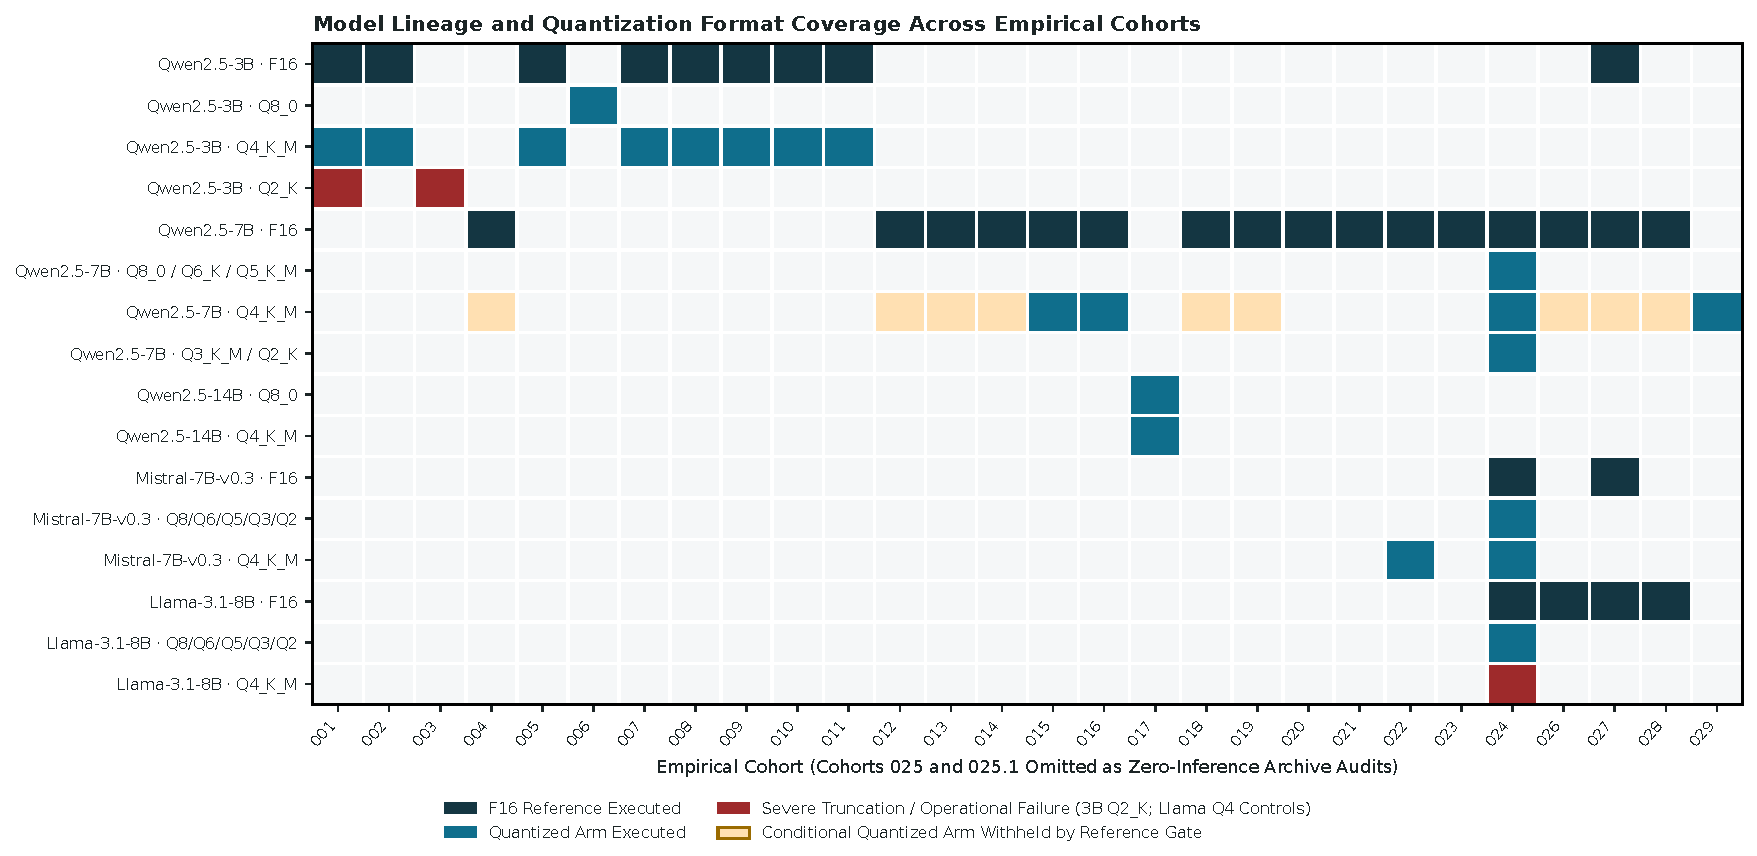
\includegraphics[width=\textwidth]{figures/fig06_model_cohort_matrix.pdf}
  \caption{Model-by-cohort deployment matrix across all 30 empirical cohorts, illustrating the progression from \texttt{Qwen2.5-3B} pilots (001--011) to \texttt{Qwen2.5-7B/14B} two-study cohorts (012--021), cross-lineage \texttt{Mistral-7B} and \texttt{Llama-3.1-8B} matrices (022--028), and the confirmatory \texttt{Qwen2.5-7B Q4\_K\_M} run (029).}
  \label{fig:model_matrix}
\end{figure}

Every run directory recorded the exact GGUF file path and, in manifest-hardened cohorts, the full 64-character SHA-256 digest of the model weights (for example, \texttt{qwen2.5-3b-instruct-f16.gguf} = \texttt{7861b687...} in Cohort~001, and \texttt{Qwen2.5-7B-Instruct-Q4\_K\_M.gguf} verified in Cohort~029's frozen manifest). In Cohort~001, \texttt{tokenizer\_metadata\_audit.json} explicitly verified that GGUF header chat templates, BOS/EOS tokens, and vocabulary tables were identical across \texttt{F16}, \texttt{Q4\_K\_M}, and \texttt{Q2\_K}, ruling out tokenizer corruption as an explanation for low-bit failures.

% =============================================================================
\section{Blind Data Contracts, Randomization, Parsing, and Logging}

Four architectural safeguards prevented subtle evaluation leakage throughout CausalFade:
\begin{enumerate}
  \item \textbf{Public-Oracle Air Gap (\texttt{D02}, \texttt{docs/DATA\_CONTRACT.md}):} Every dataset generator emitted two separate files: \texttt{public\_tasks.jsonl} (or \texttt{tasks.jsonl}), containing \emph{only} an opaque SHA-256 \texttt{task\_id} and the natural-language prompt sent to the inference runner, and \texttt{oracle\_truth.jsonl} (or \texttt{gold.jsonl}), containing the true $\ATE$, $\RD_{\mathrm{obs}}$, conflict indicator, stratum parameters, and optimal action. The inference runner never imported or opened \texttt{oracle\_truth.jsonl}.
  \item \textbf{Deterministic Counterbalancing and Permuted Schedules:} Presentation order of studies (Study~A vs.\ Study~B), study labels (randomized vs.\ historical), option order (\texttt{1 or 0} vs.\ \texttt{0 or 1}), and task dispatch schedules (\texttt{schedule.json}) were generated from fixed cryptographic or \texttt{numpy.random.Generator} seeds.
  \item \textbf{Strict Duplicate-Rejecting Parsers:} Early cohorts discovered that naive regex extraction can flatter rambling responses, whereas overly rigid bare-JSON parsing penalized \texttt{F16} Markdown code fences in Cohort~001. By Cohort~014--029, prompts explicitly forbade Markdown fences and explanations, and Cohort~029's strict parser (\texttt{json.loads(..., object\_pairs\_hook=strict)}) accepted \emph{only} a single JSON object with sole key \texttt{"activate"}, exact Python \texttt{int} value in \texttt{\{0, 1\}} (rejecting booleans, strings, floats, and duplicate JSON keys), and \texttt{finish\_reason == "stop"}.
  \item \textbf{Cryptographic Event Journaling:} Every cohort persisted raw \texttt{llama-server} JSON responses alongside latency and token counts (\texttt{raw\_responses.jsonl}). Cohort~029 elevated this to an append-only transaction log (\texttt{events.jsonl}, SHA-256 \texttt{673eb723...}) recording \texttt{intent}, \texttt{dispatch}, and \texttt{response} events with raw base64 HTTP payloads and SHA-256 digests bound to the frozen manifest.
\end{enumerate}

% =============================================================================
% Part II, Chapter 5: Pre-LLM Synthetic Validation and Cohorts 001--004
% =============================================================================
\chapter{Pre-LLM Validation and the Early 3B Backdoor Pilots (\texttt{design\_validation} and Cohorts 001--004)}\label{ch:cohorts_dv_004}

Before querying a single language model---and across its opening day of live inference on November 10, 2026---CausalFade built its synthetic backdoor generator, audited its psychometric processing tree in simulation, and ran four fast-turnaround pilot cohorts that immediately overturned naive assumptions about JSON formatting, 2-bit quantization, formula execution, and 7B scaling. Figure~\ref{fig:cohort_dep} maps the causal chain connecting all thirty-one cohort units documented in Chapters~5--12, while Table~\ref{tab:cohort_master} in Appendix~A provides a condensed cross-reference.

\begin{figure}[htbp]
  \centering
  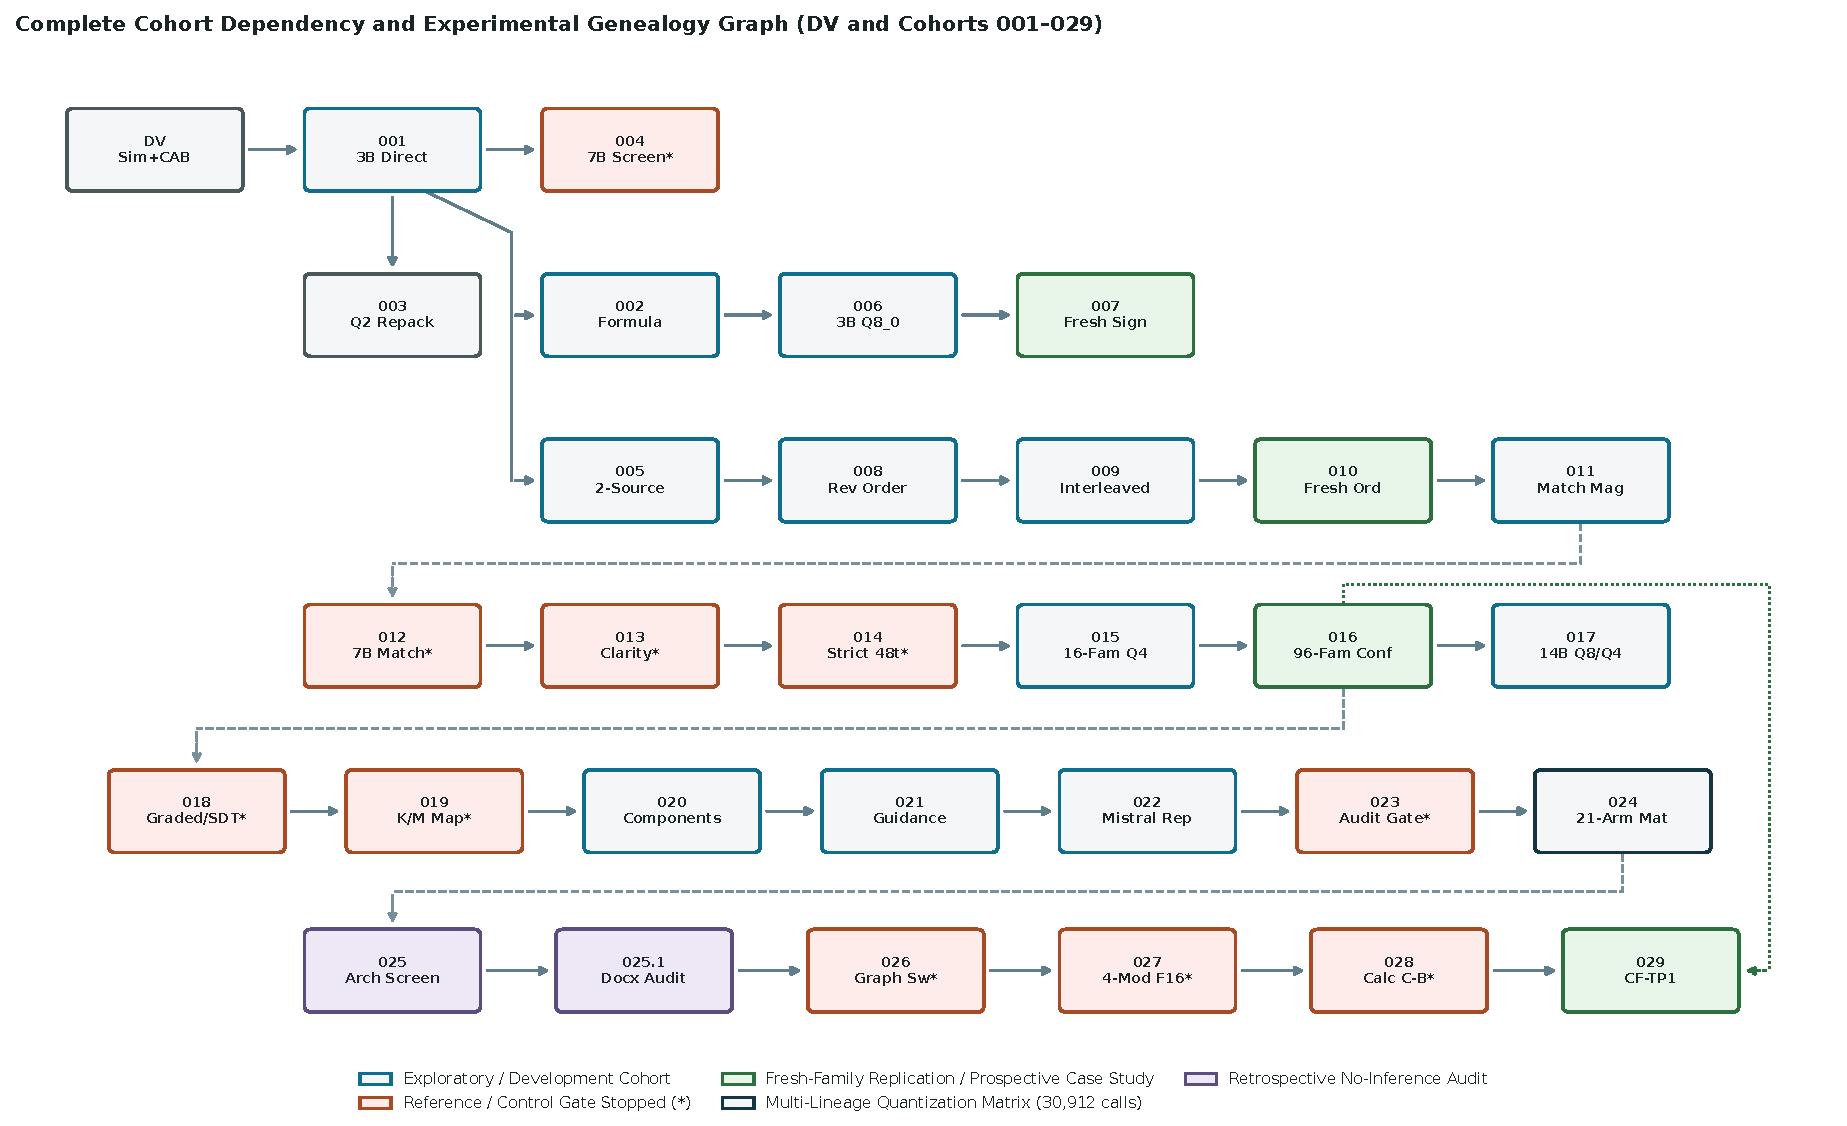
\includegraphics[width=\textwidth]{figures/fig03_cohort_dependency_graph.pdf}
  \caption{Complete cohort dependency graph from \texttt{design\_validation} through Cohort~029, showing how empirical falsifications, parser repairs, and failed reference gates drove each methodological transition.}
  \label{fig:cohort_dep}
\end{figure}

% =============================================================================
\section{Pre-LLM Suite: \texttt{design\_validation} --- Synthetic C/A/B Parameter Recovery}

\subsection*{1. Historical Context}
Following the October 28, 2026 literature scoping (\texttt{4e2fe4f}), the researchers needed to build the data-generation package (\texttt{causalfade/}) and verify that their planned statistical estimators could actually recover causal sensitivity ($C$), associative reliance ($A$), and response bias ($B$) before spending compute on local GGUF models.

\subsection*{2. Research Question}
Can an Expectation-Maximization (EM) solver accurately recover the parameters $(C, A, B)$ of a CNI-style multinomial processing tree across realistic per-cell sample sizes, and can goodness-of-fit deviance distinguish sequential tree processing from continuous logistic cue integration?

\subsection*{3. Hypothesis}
\textbf{Classification:} \emph{Exploratory synthetic validation (\texttt{H02}).} Prior to simulation, the researchers expected simplex EM estimation to recover $(C, A, B)$ reliably in interior parameter regimes and expected parametric bootstrap $G^2$ deviance tests to detect non-tree generating mechanisms.

\subsection*{4. Experimental Design}
\begin{itemize}
  \item \textbf{Independent Variables:} Six true parameter scenarios (interior, low-$C$, high-$C$ near boundary, high-$A$, extreme-$B$, null) crossed with three cell sample sizes $n_{\mathrm{cell}} \in \{50, 200, 1000\}$ ($18$ cells $\times 200$ Monte Carlo repetitions $= 3{,}600$ synthetic datasets), plus three structural model-misspecification regimes ($500$ bootstrap replicates each) and a $24$-family ($192$-prompt) baseline task fixture (\texttt{seed=20261101}).
  \item \textbf{Dependent Variables:} Parameter bias, RMSE, near-simplex-boundary rate, EM nonconvergence count, bootstrap $G^2$ $p$-values, and held-out log-loss.
  \item \textbf{Models \& Quantization:} None (pure NumPy \texttt{2.3.5} simulation; explicitly flagged in \texttt{manifest.json} as \texttt{"synthetic\_design\_validation\_not\_LLM\_results"}).
\end{itemize}

\subsection*{5. Mathematical Formulation}
Synthetic binomial counts $K_{TS} \sim \mathrm{Binomial}(n_{\mathrm{cell}}, p_{TS})$ were drawn across $(T,S) \in \{0,1\}^2$ under equation~\eqref{eq:cab_tree}, $p_{TS} = C T + (1-C)[A S + (1-A)B]$, and compared against logistic integration $p_{TS}^{\mathrm{log}} = \sigma(\beta_0 + \beta_T(2T-1) + \beta_S(2S-1))$ via likelihood-ratio deviance $G^2 = 2\sum_{T,S} \bigl[K_{TS}\ln(K_{TS}/\hat{\mu}_{TS}) + (n_{\mathrm{cell}}-K_{TS})\ln((n_{\mathrm{cell}}-K_{TS})/(n_{\mathrm{cell}}-\hat{\mu}_{TS}))\bigr]$.

\subsection*{6. Experimental Execution}
Executed deterministically on November 1, 2026 (commit \texttt{6ab18d2}) via \texttt{causalfade/cab\_tree.py} and \texttt{causalfade/generate.py}. Simultaneously, baseline deterministic policies (\texttt{exact:backdoor}, \texttt{exact:association}, \texttt{exact:random}, and $n=2{,}000$ sampled counterparts) were verified on the $192$-prompt synthetic fixture.

\subsection*{7. Results}
\emph{(Contemporaneously reported in \texttt{results/design\_validation/parameter\_recovery.json} and Figure~\ref{fig:cab_recovery}.)}
\begin{itemize}
  \item \textbf{Baseline Oracle Verification:} On the $192$-prompt fixture ($24$ families $\times 4$ $(T,S)$ cells $\times 2$ evidence modes), \texttt{backdoor} achieved $100.0\%$ accuracy ($0$ invalids), naive \texttt{association} achieved exactly $50.0\%$ ($100\%$ aligned, $0\%$ conflict), and random guessing scored $42.71\%$ (exact) and $50.0\%$ (sampled).
  \item \textbf{Parameter Recovery:} In the interior regime $(C=0.65, A=0.45, B=0.50)$, RMSE improved from $(0.0506, 0.1407, 0.1527)$ at $n_{\mathrm{cell}}=50$ to $(0.0252, 0.0703, 0.0699)$ at $n_{\mathrm{cell}}=200$ and $(0.0113, 0.0309, 0.0315)$ at $n_{\mathrm{cell}}=1000$. However, near the upper boundary ($C \to 1$), $(1-C) \to 0$ starved downstream branches of effective sample size, producing $16$ interval nonconvergences.
  \item \textbf{Observational Equivalence Discovery:} While asymmetric logistic data ($\beta_0 \neq 0$) was strongly rejected ($G^2 = 702.75$, $p_{\text{boot}} = 0.0020$), \emph{symmetric} logistic integration ($\beta_0 = 0$, generating cell probabilities $[0.0474, 0.5000, 0.5000, 0.9526]$) yielded $G^2 = 0.6876$ ($p_{\text{boot}} = 0.4331$) and virtually identical held-out log-loss ($0.4444$ tree vs.\ $0.4444$ logistic).
\end{itemize}

\subsection*{8. Interpretation at the Time}
Recorded in \texttt{VALIDATION\_REPORT.md}: $C/A/B$ trees can serve only as descriptive summaries if model fit passes, never as proof of sequential cognitive stages, and $n_{\mathrm{cell}}=16$--$50$ pilots will exhibit wide uncertainty on conditional parameters $A$ and $B$.

\subsection*{9. Retrospective Interpretation}
This pre-LLM audit prevented a major conceptual error that had appeared in prior LLM moral-psychology papers \citep{wuDeng2025counts}: recognizing symmetric logistic equivalence \emph{before} Cohort~001 meant the team was primed to check additivity ($p_{11}-p_{10}-p_{01}+p_{00}=0$) in Cohort~005 and abandon the tree cleanly when additivity failed.

\subsection*{10. Methodological Limitations}
The synthetic generator used a fixed confounding multiplier $k$, inadvertently making observational gaps $|\RD_{\mathrm{obs}}|$ larger in aligned cells ($57.10\pp$) than in conflict cells ($38.04\pp$)---an imbalance not noticed until Cohort~005 and repaired in Cohort~011.

\subsection*{11. Scientific Contribution}
\emph{Methodological refutation \& statistical improvement:} Proved 4-cell observational equivalence between CNI/$C/A/B$ trees and symmetric logistic cue integration, and validated the blind public/oracle data contract.

\subsection*{12. Transition to Subsequent Research}
Supplied the exact $16$-family development subset ($64$ exact-probability prompts) deployed in Cohort~001's first live LLM pilot.

\subsection*{13. Evidence and Reproducibility}
Artifacts: \texttt{results/design\_validation/VALIDATION\_REPORT.md}, \texttt{parameter\_recovery.json} (SHA-256 \texttt{4997af34...}), \texttt{public\_tasks.jsonl} (\texttt{ed4232a1...}), \texttt{oracle\_truth.jsonl} (\texttt{9a11f0fb...}); commit \texttt{6ab18d2}.

% =============================================================================
\section{Cohort 001: Direct Backdoor Causal Pilot on \texttt{Qwen2.5-3B}}

\subsection*{1. Historical Context}
With synthetic data generation validated and local \texttt{Qwen2.5-3B-Instruct} GGUF weights prepared on SSD (\texttt{F16}, \texttt{Q4\_K\_M}, \texttt{Q2\_K}), Cohort~001 executed the project's first live LLM experiment on November 10, 2026.

\subsection*{2. Research Question}
On exact 4-stratum confounded probability tables with an explicit causal graph ($Z\to X, Z\to Y, X\to Y$), what is \texttt{Qwen2.5-3B}'s baseline interventional accuracy and conflict penalty at \texttt{F16}, and how do \texttt{Q4\_K\_M} and \texttt{Q2\_K} alter performance?

\subsection*{3. Hypothesis}
\textbf{Classification:} \emph{Exploratory pilot of prospective hypothesis \texttt{H01}.} Expected \texttt{F16} to establish non-trivial causal competence and \texttt{Q2\_K} (and possibly \texttt{Q4\_K\_M}) to exhibit an inflated aligned-minus-conflict penalty.

\subsection*{4. Experimental Design}
\begin{itemize}
  \item \textbf{Arms:} \texttt{Qwen2.5-3B-Instruct} in \texttt{F16} (\texttt{run\_001\_f16}), \texttt{Q2\_K} (\texttt{run\_001\_q2\_k}), and \texttt{Q4\_K\_M} (\texttt{run\_001\_q4\_k\_m}).
  \item \textbf{Sample:} $16$ development families $\times 4$ $(T,S)$ cells $= 64$ exact-probability prompts per arm ($192$ total requests).
  \item \textbf{Execution Settings:} \texttt{temperature=0.0}, \texttt{max\_tokens=160}, \texttt{threads=8}, \texttt{seed=20261110}.
  \item \textbf{Required Output:} JSON with keys \texttt{ate\_estimate}, \texttt{activate}, and \texttt{adjustment\_set}.
\end{itemize}

\subsection*{5. Mathematical Formulation}
Each prompt supplied $\Prob(Y=1\mid X=x, Z=z)$ and joint cell masses $\Prob(Z=z, X=x)$ with target $\Prob(Z=0)=\Prob(Z=1)=0.5$, requiring equation~\eqref{eq:backdoor}: $\ATE = 0.5[\Prob(Y=1\mid 1,0)-\Prob(Y=1\mid 0,0)] + 0.5[\Prob(Y=1\mid 1,1)-\Prob(Y=1\mid 0,1)]$ and optimal action $\mathbb{I}(\ATE > 0)$.

\subsection*{6. Experimental Execution}
All $192$ HTTP completions succeeded and were logged to \texttt{raw\_responses.jsonl}. Representative verbatim outputs on task \texttt{6e39f6152120c3d91bc7} reveal what happened immediately:
\begin{lstlisting}
# F16 (finish_reason="stop", parse_status="invalid_json_or_response"):
```json
{
    "ate_estimate": -0.052625,
    "activate": 1,
    "adjustment_set": ["X"]
}
```
# Q2_K (finish_reason="length", 160 tokens):
\n"):\443333"4333 the"4663\n4\"6)\,\n\n\n"",...
\end{lstlisting}

\subsection*{7. Results}
\emph{(Contemporaneous statistics from \texttt{experiments/cohort\_001/summary.md} and \texttt{f16\_vs\_q4\_k\_m.json}.)}
\begin{itemize}
  \item \textbf{Strict Bare-JSON Scoring:} $0/64$ ($0.0\%$) valid across all three arms! Both \texttt{F16} and \texttt{Q4\_K\_M} wrapped all $64$ responses in Markdown \texttt{```json} fences (note: across the broader 192-item preliminary check noted in audit logs, strict bare JSON without fence stripping failed almost universally).
  \item \textbf{Single-Fence-Stripped Diagnostic Scoring:}
    \begin{itemize}
      \item \texttt{F16}: $64/64$ parseable; $33/64$ ($51.56\%$) action accuracy ($17/32$ aligned, $16/32$ conflict); recommended \texttt{activate=1} on \textbf{$63/64$ items} ($98.4\%$)! Valid adjustment set \texttt{["Z"]}: \textbf{$0/64$} (routinely emitted \texttt{["X"]} or \texttt{["Z","X"]}). Numeric ATE sign accuracy: $34/64$ ($53.1\%$, MAE $0.246$).
      \item \texttt{Q4\_K\_M}: $64/64$ parseable; $34/64$ ($53.13\%$) action accuracy; \texttt{activate=1} on $62/64$ items; numeric ATE sign accuracy: $35/64$ ($54.7\%$, MAE $0.222$).
      \item \texttt{Q2\_K}: $0/64$ parseable ($64/64$ hit the 160-token cap in repetitive digit/punctuation loops). \texttt{tokenizer\_metadata\_audit.json} confirmed GGUF tokenizer metadata matched \texttt{F16} byte-for-byte.
    \end{itemize}
\end{itemize}

\subsection*{8. Interpretation at the Time}
Cohort~001 exposed three immediate blockers: (1) strict bare-JSON parsing rejected normal chat-tuned Markdown fences; (2) \texttt{3B Q2\_K} was completely unusable due to generative looping; and (3) even \texttt{3B F16} lacked reference competence ($33/64 \approx$ chance, $63/64$ \texttt{activate=1}, $0/64$ adjustment set, and frequent disagreement between negative \texttt{ate\_estimate: -0.052625} and \texttt{activate: 1}!).

\subsection*{9. Retrospective Interpretation}
Look closely at the verbatim \texttt{F16} response above: on its very first item in the entire project, \texttt{Qwen2.5-3B F16} estimated a \emph{negative} treatment effect (\texttt{-0.052625}) and simultaneously set \texttt{"activate": 1}! Every major theme of CausalFade---parser artifacts, action-prior dominance, numeric-action dissociation, and reference-model incompetence---was already visible in embryo in Cohort~001.

\subsection*{10. Methodological Limitations}
Small 3B capacity, 3-field output complexity, Markdown fence mismatch, and reuse of $16$ development families.

\subsection*{11. Scientific Contribution}
\emph{Infrastructure discovery \& negative baseline finding:} Motivated fence-aware secondary diagnostics (\texttt{D03}), proved \texttt{3B Q2\_K} token-loop collapse, and uncovered extreme \texttt{activate=1} bias alongside numeric-action inconsistency.

\subsection*{12. Transition to Subsequent Research}
Spawned three parallel diagnostic branches on the same day: Cohort~002 (supplying the explicit arithmetic formula to separate causal identification from calculation), Cohort~003 (testing whether \texttt{llama-server} CPU repacking caused \texttt{Q2\_K}'s collapse), and Cohort~004 (testing whether scaling to \texttt{Qwen2.5-7B F16} solved the direct backdoor task).

\subsection*{13. Evidence and Reproducibility}
Artifacts: \texttt{experiments/cohort\_001/summary.md}, \texttt{f16\_vs\_q2\_k.json}, \texttt{f16\_vs\_q4\_k\_m.json}, \texttt{tokenizer\_metadata\_audit.json}, \texttt{run\_001\_*/raw\_responses.jsonl}; commit \texttt{0333c67}.

% =============================================================================
\section{Cohort 002: Formula-Given Arithmetic Control on \texttt{Qwen2.5-3B}}

\subsection*{1. Historical Context}
In Cohort~001, \texttt{Qwen2.5-3B} failed both causal adjustment-set selection ($0/64$) and numerical ATE estimation ($34/64$ sign accuracy). Before blaming ``causal reasoning,'' the researchers asked whether the 3B model could even compute the backdoor weighted average when handed the exact formula explicitly.

\subsection*{2. Research Question}
If the causal graph narrative is replaced by the explicit algebraic standardization formula on the exact same $64$ numerical tables, do \texttt{F16} and \texttt{Q4\_K\_M} compute accurate ATE signs and flip their binary actions accordingly?

\subsection*{3. Hypothesis}
\textbf{Classification:} \emph{Exploratory control (\texttt{H04}).} Expected explicit formula provision to boost both numeric ATE estimation and explicit action accuracy.

\subsection*{4. Experimental Design}
\begin{itemize}
  \item \textbf{Arms:} \texttt{Qwen2.5-3B-Instruct} \texttt{F16} (\texttt{run\_001\_f16}) and \texttt{Q4\_K\_M} (\texttt{run\_002\_q4\_k\_m}).
  \item \textbf{Sample:} Identical $16$ families ($64$ tables/arm, $128$ total requests) and task IDs from Cohort~001, replacing causal story prose with the explicit weighted-difference formula while keeping the 3-key JSON contract.
\end{itemize}

\subsection*{5. Mathematical Formulation}
Direct evaluation of $\hat{\tau} = 0.5[p_{10} - p_{00}] + 0.5[p_{11} - p_{01}]$ from supplied stratum probabilities $p_{xz} = \Prob(Y=1\mid X=x, Z=z)$, compared on (i) explicit binary decision $\hat{a} \in \{0,1\}$, (ii) numeric sign accuracy $\mathbb{I}(\sign(\hat{\tau}) = \sign(\tau))$, and (iii) internal disagreement $\mathbb{I}(\hat{a} \neq \mathbb{I}(\hat{\tau} > 0))$.

\subsection*{6. Experimental Execution}
Completed November 10, 2026 (\texttt{temperature=0.0}, \texttt{max\_tokens=160}). All $128$ responses stopped normally inside single \texttt{```json} fences ($0/64$ strict bare JSON; $64/64$ fence-valid).

\subsection*{7. Results}
\emph{(Contemporaneous metrics from \texttt{experiments/cohort\_002/summary.md} and Figure~\ref{fig:control_arch}A.)}
\begin{itemize}
  \item \textbf{Numeric ATE Sign Accuracy Surged---and Diverged by Precision:} \texttt{F16} jumped from $34/64$ (Cohort~001) to \textbf{$61/64$ ($95.31\%$)} (MAE dropping from $0.246$ to $0.062$), whereas \texttt{Q4\_K\_M} rose only from $35/64$ to \textbf{$45/64$ ($70.31\%$)} (MAE $0.081$). Post-hoc sign-derived policy accuracy differed by \textbf{$-25.00\pp$} under \texttt{Q4\_K\_M} vs.\ \texttt{F16} (paired 16-family percentile 95\% CI $[-37.50, -10.94]\pp$), spread evenly across aligned ($-7$ items) and conflict ($-9$ items; conflict-penalty shift $+6.25\pp$, CI $[-9.38, +21.88]\pp$).
  \item \textbf{Complete Polarity Flip in Explicit Binary Actions:} Whereas Cohort~001 \texttt{F16} chose \texttt{activate=1} on $63/64$ items, Cohort~002 \texttt{F16} chose \texttt{activate=1} on \textbf{$0/64$ items} ($100\%$ \texttt{activate=0}, scoring $32/64 = 50.0\%$)! \texttt{Q4\_K\_M} chose \texttt{activate=1} on $3/64$ items ($35/64 = 54.69\%$). Consequently, explicit actions \emph{disagreed with the model's own numeric ATE sign} on $29/64$ (\texttt{F16}) and $48/64$ (\texttt{Q4\_K\_M}) items!
\end{itemize}

\begin{figure}[htbp]
  \centering
  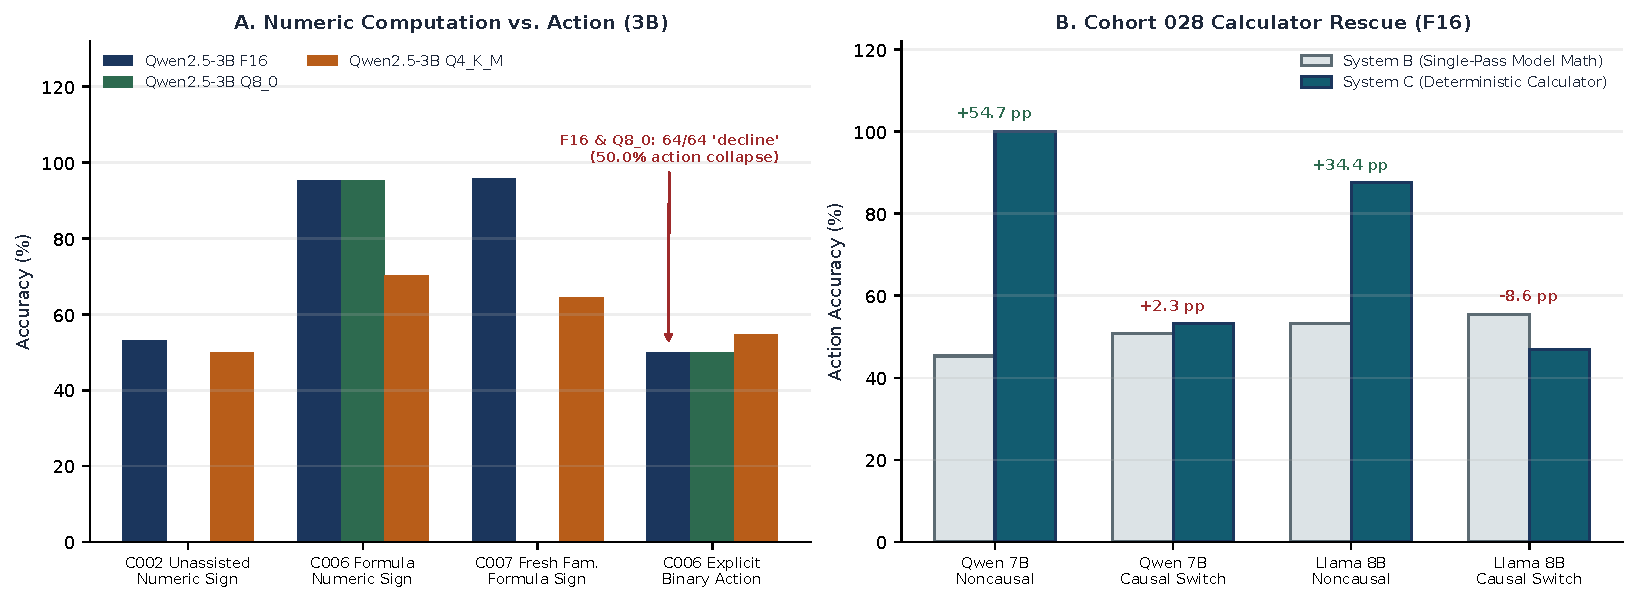
\includegraphics[width=\textwidth]{figures/fig12_experimental_control_architecture.pdf}
  \caption{Control-task dissociations across CausalFade: (A) Numeric ATE sign accuracy vs.\ explicit binary action collapse across Cohorts~002, 006, and 007 on \texttt{Qwen2.5-3B}; (B) Cohort~028 deterministic calculator rescue on noncausal named-rule tasks vs.\ null effect on causal graph-switch tasks.}
  \label{fig:control_arch}
\end{figure}

\subsection*{8. Interpretation at the Time}
Documented in \texttt{experiments/cohort\_002/summary.md}: (1) \texttt{3B F16} \emph{can} execute backdoor arithmetic ($61/64$) when told which formula to compute, proving Cohort~001's failure was an identification/formulation bottleneck rather than raw inability to add four numbers; (2) \texttt{3B Q4\_K\_M} exhibits a candidate $-25\pp$ arithmetic-execution deficit under this scaffold (not a selective causal-conflict deficit); and (3) explicit binary decisions in 3-key JSON are completely decoupled from numeric estimates and flip wildly ($63/64 \to 0/64$ \texttt{activate}) with prompt wording.

\subsection*{9. Retrospective Interpretation}
Cohort~002 produced the single strongest genuine quantization difference in the entire CausalFade archive ($-25\pp$, later replicated at $-31.25\pp$ in Cohort~007)---and crucially, it occurred on \emph{explicit formula execution} equally across aligned and conflict cells, confirming \citet{li2025meets} (low-bit arithmetic degradation) rather than \texttt{H01} (selective causal confounding fallback).

\subsection*{10. Methodological Limitations}
Reused Cohort~001's 16 development families; sign scoring was formulated post-hoc after observing the $0/64$ action collapse; Markdown fences persisted.

\subsection*{11. Scientific Contribution}
\emph{Positive empirical finding (arithmetic quantization drop) \& benchmark artifact discovery (numeric-vs.-action dissociation).}

\subsection*{12. Transition to Subsequent Research}
Prompted Cohort~006 (\texttt{Q8\_0} intermediate precision check) and Cohort~007 (prospective fresh-family replication of the formula-sign deficit).

\subsection*{13. Evidence and Reproducibility}
Artifacts: \texttt{experiments/cohort\_002/summary.md}, \texttt{f16\_vs\_q4\_k\_m\_formula.json}, \texttt{estimate\_sign\_policy\_sensitivity.json}; commit \texttt{f2b2cb1}.

% =============================================================================
\section{Cohort 003: \texttt{llama.cpp} CPU Weight-Repacking Diagnostic on \texttt{3B Q2\_K}}

\subsection*{1. Historical Context}
In Cohort~001, \texttt{Qwen2.5-3B Q2\_K} emitted $64/64$ length-capped gibberish loops. Before declaring 2-bit compression unusable at 3B scale, good systems hygiene required testing whether \texttt{llama-server}'s runtime CPU tensor repacking kernel corrupted \texttt{Q2\_K} dequantization on the host processor.

\subsection*{2. Research Question}
Does passing \texttt{--no-repack} to \texttt{llama-server} eliminate or reduce \texttt{Qwen2.5-3B Q2\_K}'s token-looping collapse?

\subsection*{3. Hypothesis}
\textbf{Classification:} \emph{Technical diagnostic (\texttt{H03}).} Tested whether runtime SIMD weight repacking caused the \texttt{Q2\_K} failure.

\subsection*{4. Experimental Design}
Two arms on \texttt{qwen2.5-3b-instruct-q2\_k.gguf}: \texttt{run\_001\_default} (default CPU repacking) vs.\ \texttt{run\_002\_no\_repack} (\texttt{--no-repack}), evaluated on the first $4$ development families ($16$ exact prompts/arm, $32$ total requests; \texttt{max\_tokens=160}, \texttt{temperature=0.0}).

\subsection*{5. Mathematical Formulation}
Floating-point matrix-vector multiplication is non-associative in finite SIMD registers; changing memory layout (\texttt{repack} vs.\ \texttt{--no-repack}) alters summation order at machine epsilon $\mathcal{O}(2^{-24})$, which can diverge chaotically once argmax ties occur in an unstable low-bit trajectory.

\subsection*{6. Experimental Execution}
Completed November 10, 2026 (commit \texttt{941cf7e}). Compare verbatim outputs on identical task \texttt{3e459f5e3dcade7fc172}:
\begin{lstlisting}
# run_001_default (length-capped):
\n"43)366323\n43\"333364333333643333334333333333...
# run_002_no_repack (length-capped):
\n"43)366323\n43)\n436363663663663366333646363333...
\end{lstlisting}

\subsection*{7. Results}
Both \texttt{run\_001\_default} and \texttt{run\_002\_no\_repack} scored \textbf{$0/16$ valid} ($0.0\%$) and hit \texttt{finish\_reason="length"} on \textbf{$16/16$ items} ($100\%$). Interestingly, exact output strings diverged after the first $\sim 12$ characters on $16/16$ items (confirming floating-point reduction-order sensitivity), but neither kernel produced coherent English or JSON.

\subsection*{8. Interpretation at the Time}
\texttt{3B Q2\_K} collapse is intrinsic to uncalibrated 2-bit weight quantization of \texttt{Qwen2.5-3B-Instruct}, not a \texttt{llama.cpp} CPU repacking bug.

\subsection*{9. Retrospective Interpretation}
A textbook systems control: had the team skipped Cohort~003, a skeptical reviewer could reasonably have blamed SIMD kernel bugs for low-bit failure. Later, Cohort~024 showed that at $7\text{B}$--$8\text{B}$ scale, \texttt{Q2\_K} achieved $99.7\%$--$100\%$ strict JSON validity across Qwen, Mistral, and Llama, confirming that severe syntactic collapse at \texttt{Q2\_K} was specific to small 3B model capacity under uncalibrated PTQ \citep{alimaskina2026extreme}.

\subsection*{10. Methodological Limitations}
Tested one \texttt{Q2\_K} artifact built without an importance matrix (\texttt{imatrix}).

\subsection*{11. Scientific Contribution}
\emph{Infrastructure discovery:} Ruled out inference-engine repacking artifacts and justified retiring \texttt{3B Q2\_K}.

\subsection*{12. Transition to Subsequent Research}
Closed the \texttt{3B Q2\_K} investigation and shifted focus to \texttt{Q4\_K\_M}, \texttt{Q8\_0}, and larger 7B models.

\subsection*{13. Evidence and Reproducibility}
Artifacts: \texttt{experiments/cohort\_003/summary.md}, \texttt{repack\_comparison.json}, \texttt{run\_001\_default/}, \texttt{run\_002\_no\_repack/}; commit \texttt{941cf7e}.

% =============================================================================
\section{Cohort 004: \texttt{Qwen2.5-7B F16} Direct-Table Reference Competence Screen}

\subsection*{1. Historical Context}
Since \texttt{Qwen2.5-3B F16} scored at chance ($33/64$) and $0/64$ on adjustment sets in Cohort~001, the researchers introduced an explicit methodological rule (\texttt{D04}): \emph{before evaluating quantized arms on a new model or task, the unquantized \texttt{F16} reference must pass a pre-declared competence gate}. Cohort~004 applied this gate to \texttt{Qwen2.5-7B-Instruct F16}.

\subsection*{2. Research Question}
Does scaling parameter count from $3\text{B}$ to $7\text{B}$ at \texttt{F16} enable reliable direct causal decisions ($\ge 22/32$ overall accuracy) on the Cohort~001 4-stratum backdoor table prompt?

\subsection*{3. Hypothesis}
\textbf{Classification:} \emph{Documented prospective feasibility gate.} Pre-specified threshold: overall fence-stripped accuracy $\ge 22/32$ ($68.75\%$) required before running \texttt{7B Q2\_K} or \texttt{7B Q4\_K\_M}.

\subsection*{4. Experimental Design}
Single arm (\texttt{Qwen2.5-7B-Instruct F16}) on $8$ development families ($32$ exact-probability prompts: $16$ aligned, $16$ conflict; \texttt{max\_tokens=160}, \texttt{temperature=0.0}).

\subsection*{5. Mathematical Formulation}
Identical 4-stratum backdoor adjustment target~\eqref{eq:backdoor} as Cohort~001.

\subsection*{6. Experimental Execution}
Completed November 10, 2026 (commit \texttt{01c7590}); all $32$ responses finished normally inside \texttt{```json} fences.

\subsection*{7. Results}
\begin{itemize}
  \item \textbf{Graph Identification Improved Dramatically:} Unlike \texttt{3B F16} ($0/64$), \texttt{7B F16} output the exact valid backdoor adjustment set \texttt{["Z"]} on \textbf{$32/32$ items ($100\%$)}!
  \item \textbf{Action Gate Failed Due to \texttt{activate=1} Bias:} Despite naming \texttt{["Z"]} correctly on every item, \texttt{7B F16} recommended \texttt{activate=1} on \textbf{$31/32$ items ($96.9\%$)}, yielding \textbf{$17/32$ ($53.13\%$)} overall action accuracy ($8/16$ aligned, $9/16$ conflict)---failing the $\ge 22/32$ gate. Strict bare-JSON accuracy was $0/32$.
\end{itemize}

\subsection*{8. Interpretation at the Time}
Scaling to 7B solved symbolic adjustment-set naming (\texttt{["Z"]} $32/32$) but left end-to-end table standardization and binary decision-making trapped in a $97\%$ \texttt{activate=1} default policy. Per the pre-declared gate, quantized 7B runs were withheld.

\subsection*{9. Retrospective Interpretation}
Cohort~004 provided the first glimpse of a pattern that recurred in Cohorts~021 and 027: \emph{declarative causal graph knowledge (\texttt{["Z"]} = 100\%) does not mean a language model applies that graph when computing an action}.

\subsection*{10. Methodological Limitations}
Small $8$-family ($32$-item) screen; bundled multi-step arithmetic with causal identification in one pass without scratchpad tokens.

\subsection*{11. Scientific Contribution}
\emph{Negative result \& methodological gate enforcement:} Demonstrated declarative-vs.-procedural causal dissociation at 7B and enforced the reference-competence gate for the first time.

\subsection*{12. Transition to Subsequent Research}
Because direct 4-cell backdoor arithmetic blocked both 3B and 7B references, Cohort~005 simplified the task by pre-computing the interventional and historical summary rates directly into a two-study source-selection problem.

\subsection*{13. Evidence and Reproducibility}
Artifacts: \texttt{experiments/cohort\_004/summary.md}, \texttt{run\_001\_f16/results.json}, \texttt{raw\_responses.jsonl}; commit \texttt{01c7590}.

% =============================================================================
% Part II, Chapter 6: Cohorts 005--007
% =============================================================================
\chapter{Processing-Tree Falsification and Formula-Assisted Dissociation (Cohorts 005--007)}\label{ch:cohorts_005_007}

Having discovered in Cohorts~001--004 that direct 4-stratum backdoor tables overwhelmed single-pass decision accuracy even at \texttt{7B F16}, while explicit formulas in Cohort~002 exposed a sharp $-25\pp$ \texttt{Q4\_K\_M} numeric sign drop alongside a $0/64$ action collapse, the researchers pursued two focused questions in Cohorts~005--007: (1) What happens when arithmetic is removed by supplying pre-aggregated randomized and historical rates directly, and does the CNI/$C/A/B$ processing tree fit real LLM choices? (2) Does the formula-execution drop at \texttt{3B Q4\_K\_M} spare \texttt{Q8\_0} and replicate prospectively on fresh SCM families?

% =============================================================================
\section{Cohort 005: Supplied-Rate Source Selection and C/A/B Tree Falsification}

\subsection*{1. Historical Context}
In Cohorts~001 and 004, models failed to compute $\Prob(Y=1\mid \doop(X=x))$ from stratified observational tables. Cohort~005 stripped away stratum arithmetic entirely: each prompt supplied both the exact randomized-trial rates (identifying $\Prob(Y=1\mid \doop(X=x))$) and the confounded historical rates ($\Prob(Y=1\mid X=x)$), asking only for binary JSON \texttt{\{"activate": 0/1\}}.

\subsection*{2. Research Question}
When interventional and observational rates are supplied directly without stratum arithmetic, can \texttt{Qwen2.5-3B F16} select the randomized source over confounded history, how does \texttt{Q4\_K\_M} compare, and do observed $2\times 2$ cell rates satisfy the $C/A/B$ multinomial processing tree?

\subsection*{3. Hypothesis}
\textbf{Classification:} \emph{Exploratory diagnostic of \texttt{H01} and \texttt{H02}.} Expected \texttt{F16} to prefer randomized trial evidence, \texttt{Q4\_K\_M} to exhibit a larger conflict penalty, and $2\times 2$ activation rates to satisfy $p_{11} - p_{10} - p_{01} + p_{00} = 0$.

\subsection*{4. Experimental Design}
\begin{itemize}
  \item \textbf{Arms:} \texttt{Qwen2.5-3B-Instruct} \texttt{F16} (\texttt{run\_001\_f16}) and \texttt{Q4\_K\_M} (\texttt{run\_001\_q4\_k\_m}).
  \item \textbf{Sample:} $16$ development families $\times 4$ $(T,S)$ cells $= 64$ single-key prompts/arm ($128$ total requests). Study display order (randomized-first vs.\ historical-first) was assigned at the family level.
\end{itemize}

\subsection*{5. Mathematical Formulation}
Under the homogeneous $C/A/B$ tree~\eqref{eq:cab_tree}, activation rates $p_{TS} = \Prob(\text{act}=1\mid T,S)$ must satisfy $\mathcal{I}_{\mathrm{tree}} = p_{11} - p_{10} - p_{01} + p_{00} = 0$, and the aligned-minus-conflict accuracy penalty equals $w_A = (1-C)A$ only when $B$ does not interact with cell order.

\subsection*{6. Experimental Execution}
Completed November 10, 2026 (commit \texttt{4e90b24}). Every output stopped normally in $14$ tokens with a single fenced JSON object (\texttt{```json ... \{"activate": 1\} ```}; $0/64$ strict bare JSON, $64/64$ single-fence valid).

\subsection*{7. Results}
\emph{(Contemporaneous statistics from \texttt{experiments/cohort\_005/summary.md} and \texttt{source\_and\_tree\_diagnostics.json}.)}
\begin{itemize}
  \item \textbf{Paradoxical Reversal of the Conflict Penalty:}
    \begin{itemize}
      \item \texttt{F16}: $39/64$ ($60.94\%$) overall, with \textbf{$28/32$ ($87.50\%$)} aligned vs.\ \textbf{$11/32$ ($34.38\%$)} conflict ($\mathrm{ConflictPenalty}(\text{\texttt{F16}}) = +53.125\pp$), choosing \texttt{activate=1} on $47/64$ items and following the misleading historical direction on $21/32$ conflict items!
      \item \texttt{Q4\_K\_M}: $35/64$ ($54.69\%$) overall, with \textbf{$19/32$ ($59.38\%$)} aligned vs.\ \textbf{$16/32$ ($50.00\%$)} conflict ($\mathrm{ConflictPenalty}(\text{\texttt{Q4\_K\_M}}) = +9.375\pp$), choosing \texttt{activate=1} on \textbf{$61/64$ items ($95.3\%$)}!
      \item Thus $\Delta(\text{\texttt{Q4\_K\_M}}) = \mathrm{ConflictPenalty}(\text{\texttt{Q4\_K\_M}}) - \mathrm{ConflictPenalty}(\text{\texttt{F16}}) = \mathbf{-43.75\pp}$ (paired 16-family percentile 95\% CI $[-65.63, -21.88]\pp$)---the \emph{exact opposite sign} of founding hypothesis \texttt{H01}, driven entirely by \texttt{Q4\_K\_M} collapsing to near-constant activation!
    \end{itemize}
  \item \textbf{Decisive Empirical Falsification of the $C/A/B$ Tree:} On \texttt{F16}, the additivity residual $\widehat{\mathcal{I}}_{\mathrm{tree}} = \hat{p}_{11} - \hat{p}_{10} - \hat{p}_{01} + \hat{p}_{00}$ was \textbf{$-43.75\pp$} (paired 16-family 95\% CI $[-68.75, -18.75]\pp$; \texttt{Q4\_K\_M} residual $-18.75\pp$, CI $[-37.50, 0.00]\pp$).
  \item \textbf{Discovery of Two Structural Confounds:} Post-hoc inspection in \texttt{summary.md} caught two critical clues: (i) when historical evidence was listed first ($10$ conflict items), \texttt{F16} followed history on $10/10$ ($0\%$ conflict accuracy), whereas when randomized evidence was listed first ($22$ conflict items), \texttt{F16} activated on $22/22$ ($11/22$ correct); and (ii) the original generator produced larger observational gaps in aligned items ($57.10\pp$) than in conflict items ($38.04\pp$) despite matched $9.53\pp$ causal gaps.
\end{itemize}

\subsection*{8. Interpretation at the Time}
Cohort~005 was an immediate intellectual watershed (\texttt{D05}): the researchers explicitly rejected interpreting \texttt{Q4\_K\_M}'s $-43.75\pp$ smaller conflict penalty as ``better causal reasoning,'' formally retired homogeneous $C/A/B$ processing-tree parameter reporting due to the $-43.75\pp$ additivity failure, and flagged both within-item presentation order and observational-gap imbalance for dedicated follow-up.

\subsection*{9. Retrospective Interpretation}
Few moments in CausalFade better illustrate scientific integrity. A careless team looking only at conflict accuracy ($16/32$ \texttt{Q4\_K\_M} vs.\ $11/32$ \texttt{F16}) or $\Delta(\text{\texttt{Q4\_K\_M}}) = -43.75\pp$ might have spun a flashy claim that ``quantization acts as regularization against confounding.'' Checking total activation counts ($61/64$) and tree additivity immediately exposed that illusion.

\subsection*{10. Methodological Limitations}
Presentation order was assigned at the family level rather than crossed within each item; observational gap magnitudes differed between aligned and conflict cells.

\subsection*{11. Scientific Contribution}
\emph{Methodological refutation (\texttt{H02} $C/A/B$ tree retired) \& benchmark artifact discovery (action-bias inversion of $\mathrm{ConflictPenalty}$, order sensitivity, and aligned/conflict gap asymmetry).}

\subsection*{12. Transition to Subsequent Research}
Directly motivated Cohorts~008--010 (within-item source-order reversal) and Cohort~011 (matched observational-strength generator).

\subsection*{13. Evidence and Reproducibility}
Artifacts: \texttt{experiments/cohort\_005/summary.md}, \texttt{f16\_vs\_q4\_k\_m\_source\_selection.json}, \texttt{source\_and\_tree\_diagnostics.json}; commit \texttt{4e90b24}.

% =============================================================================
\section{Cohort 006: \texttt{3B Q8\_0} Intermediate-Precision Formula Follow-Up}

\subsection*{1. Historical Context}
Cohort~002 had found a $-25.0\pp$ drop in numeric ATE sign accuracy from \texttt{3B F16} ($61/64$) to \texttt{3B Q4\_K\_M} ($45/64$) when the backdoor formula was explicitly provided. Before testing fresh families, the researchers checked whether moderate 8-bit quantization (\texttt{Q8\_0}, $\approx 8.5\;\BPW$) preserved \texttt{F16}'s numeric execution.

\subsection*{2. Research Question}
Does \texttt{Qwen2.5-3B Q8\_0} match \texttt{F16} or degrade toward \texttt{Q4\_K\_M} on formula-given numeric ATE sign accuracy and explicit binary action selection?

\subsection*{3. Hypothesis}
\textbf{Classification:} \emph{Exploratory intermediate-precision check (\texttt{H04}).} Based on \citet{liu2025hurts}, expected 8-bit quantization to preserve \texttt{F16} arithmetic closely while outperforming \texttt{Q4\_K\_M}.

\subsection*{4. Experimental Design}
Single new arm (\texttt{qwen2.5-3b-instruct-q8\_0.gguf}, \texttt{run\_001\_q8\_0}) executed on the exact $64$-prompt Cohort~002 schedule and compared paired-by-task against archived Cohort~002 \texttt{F16} and \texttt{Q4\_K\_M}.

\subsection*{5. Mathematical Formulation}
Identical explicit standardization formula $\hat{\tau} = 0.5(p_{10}-p_{00}) + 0.5(p_{11}-p_{01})$ as Cohort~002.

\subsection*{6. Experimental Execution}
Completed November 10, 2026 (commit \texttt{09cf43b}); all $64$ responses stopped normally inside single \texttt{```json} fences ($0/64$ strict bare JSON; $64/64$ fence-valid).

\subsection*{7. Results}
\begin{itemize}
  \item \textbf{Exact Tie With \texttt{F16} on Numeric Signs:} \texttt{Q8\_0} achieved \textbf{$61/64$ ($95.31\%$)} correct ATE signs ($29/32$ aligned, $32/32$ conflict)---tying \texttt{F16} ($61/64$, paired difference $0.00\pp$, 16-family percentile 95\% CI $[-4.69, +4.69]\pp$, with $1$ item gained and $1$ lost) and outperforming \texttt{Q4\_K\_M} ($45/64$) by \textbf{$+25.00\pp$} (95\% CI $[+12.50, +35.94]\pp$).
  \item \textbf{Identical $100\%$ Decline Collapse on Actions:} Like \texttt{F16}, \texttt{Q8\_0} output \texttt{"activate": 0} on \textbf{$64/64$ items}, scoring $32/64$ ($50.0\%$) on explicit actions and disagreeing with its own positive numeric ATE estimates on $29/64$ items!
\end{itemize}

\subsection*{8. Interpretation at the Time}
Confirmed that the 3B formula-execution degradation occurs between $8$-bit (\texttt{Q8\_0}) and $4$-bit (\texttt{Q4\_K\_M}) compression, while proving that the $100\%$ \texttt{decline} action collapse is an architecture/prompt-level behavior shared across \texttt{F16} and \texttt{Q8\_0}.

\subsection*{9. Retrospective Interpretation}
Reinforces two consistent lessons: 8-bit GGUF quantization (\texttt{Q8\_0}) was behaviorally indistinguishable from \texttt{F16} on formula execution, and numeric estimation vs.\ binary commitment behaved as two separate output heads under multi-key JSON prompts.

\subsection*{10. Methodological Limitations}
Reused the $16$ development families from Cohorts~001--002; single-fence parsing required.

\subsection*{11. Scientific Contribution}
\emph{Positive empirical finding (localized arithmetic drop to $<8$ bits) \& replication of numeric-action dissociation.}

\subsection*{12. Transition to Subsequent Research}
Because Cohorts~002 and 006 both reused the original $16$ development families, Cohort~007 tested whether the \texttt{F16}-vs.-\texttt{Q4\_K\_M} formula-sign gap replicated prospectively on freshly sampled SCM families.

\subsection*{13. Evidence and Reproducibility}
Artifacts: \texttt{experiments/cohort\_006/summary.md}, \texttt{run\_001\_f16\_vs\_q8\_0\_estimate\_sign.json}, \texttt{run\_002\_q4\_k\_m\_vs\_q8\_0\_estimate\_sign.json}; commit \texttt{09cf43b}.

% =============================================================================
\section{Cohort 007: Fresh-Family Replication of the \texttt{3B} Formula-Sign Deficit}

\subsection*{1. Historical Context}
In Cohort~002, scoring the sign of \texttt{ate\_estimate} had been introduced post-hoc after observing explicit action collapse. Scientific rigor required testing that metric \emph{prospectively} on newly generated families untouched by prior prompt tuning.

\subsection*{2. Research Question}
Does \texttt{Qwen2.5-3B Q4\_K\_M}'s deficit in formula-given numeric ATE sign accuracy relative to \texttt{F16} replicate on an independent sample of fresh SCM families?

\subsection*{3. Hypothesis}
\textbf{Classification:} \emph{Documented prospective fresh-family replication (\texttt{H04}).} Predicted $\mathrm{SignAcc}(\text{\texttt{Q4\_K\_M}}) < \mathrm{SignAcc}(\text{\texttt{F16}})$ on fresh worlds without claiming selective causal-conflict vulnerability.

\subsection*{4. Experimental Design}
\begin{itemize}
  \item \textbf{Arms:} \texttt{Qwen2.5-3B-Instruct} \texttt{F16} (\texttt{run\_001\_f16}) and \texttt{Q4\_K\_M} (\texttt{run\_001\_q4\_k\_m}).
  \item \textbf{Sample:} $12$ freshly generated SCM families (\texttt{seed=20261111}) $\times 4$ $(T,S)$ cells $= 48$ formula-assisted prompts/arm ($96$ total requests).
\end{itemize}

\subsection*{5. Mathematical Formulation}
Paired family-cluster mean difference $\widehat{\Delta}_{\mathrm{sign}} = \frac{1}{12}\sum_{i=1}^{12} (\bar{Y}_{i,\text{\texttt{Q4}}} - \bar{Y}_{i,\text{\texttt{F16}}})$ over $4$-item family clusters, with paired percentile bootstrap 95\% confidence intervals.

\subsection*{6. Experimental Execution}
Completed November 10, 2026 (commit \texttt{12c7667}); $96/96$ normal stops inside single \texttt{```json} fences.

\subsection*{7. Results}
\begin{itemize}
  \item \textbf{Prospective Replication Confirmed:} \texttt{F16} achieved \textbf{$46/48$ ($95.83\%$)} numeric ATE sign accuracy vs.\ \texttt{Q4\_K\_M\textbf{'s }$31/48$ ($64.58\%$)\textbf{---a paired difference of }$-31.25\pp$} (95\% paired family CI $[-41.67, -20.83]\pp$), exceeding Cohort~002's $-25.00\pp$ developmental effect!
  \item \textbf{Action Collapse Persisted Unchanged:} Explicit binary actions remained stuck at chance due to \texttt{decline} bias: \texttt{F16} scored \textbf{$24/48$ ($50.00\%$)} ($0/48$ \texttt{activate=1}) and \texttt{Q4\_K\_M} scored \textbf{$28/48$ ($58.33\%$)}.
\end{itemize}

\subsection*{8. Interpretation at the Time}
Established a genuine, prospectively replicated 4-bit quantization degradation in 3B multi-term decimal formula evaluation, while confirming that explicit binary action fields remained unusable under the 3-key formula scaffold.

\subsection*{9. Retrospective Interpretation}
Cohort~007 stands as one of only two cleanly replicated quantization effects across all 29 cohorts (alongside Cohort~016's 7B order effect)---and notably, it is a \emph{noncausal arithmetic execution effect}, not a causal identification effect.

\subsection*{10. Methodological Limitations}
Restricted to one 3B checkpoint family and explicit algebraic instructions rather than autonomous causal reasoning.

\subsection*{11. Scientific Contribution}
\emph{Positive empirical finding:} Prospectively replicated $-31.25\pp$ 4-bit arithmetic sign degradation on fresh families while confirming persistent numeric-action dissociation.

\subsection*{12. Transition to Subsequent Research}
Having closed the 3B formula-arithmetic loop, the researchers returned to Cohort~005's unfinished causal question: why did two-study source selection shift so sharply with presentation order?

\subsection*{13. Evidence and Reproducibility}
Artifacts: \texttt{experiments/cohort\_007/summary.md}, \texttt{f16\_vs\_q4\_k\_m\_fresh\_formula.json}, \texttt{run\_001\_*/raw\_responses.jsonl}; commit \texttt{12c7667}.

% =============================================================================
% Part II, Chapter 7: Cohorts 008--012
% =============================================================================
\chapter{Source-Order Crossovers, Matched-Strength Repair, and 7B Feasibility (Cohorts 008--012)}\label{ch:cohorts_008_012}

Cohort~005 had hinted that \texttt{Qwen2.5-3B F16} changed its conflict choices depending on whether randomized or historical rates appeared first---and had simultaneously exposed a generator asymmetry where aligned historical gaps ($57.10\pp$) were wider than conflict historical gaps ($38.04\pp$). Between November 10 and November 12, 2026, Cohorts~008--012 systematically isolated within-item presentation order, survived a mid-run workstation shutdown and a post-hoc count-display bug, repaired the observational-gap generator flaw, and screened \texttt{Qwen2.5-7B F16} on the repaired two-study task.

% =============================================================================
\section{Cohort 008: Within-Item Source-Order Reversal (and Interrupted Run Recovery)}

\subsection*{1. Historical Context}
In Cohort~005, presentation order had been assigned at the \emph{family} level ($10$ historical-first vs.\ $22$ randomized-first conflict items), confounding item parameters with line order. Cohort~008 reversed the study line order on the exact same $64$ Cohort~005 items so every item served as its own control.

\subsection*{2. Research Question}
When study presentation order is reversed within the exact same 64 items, does \texttt{Qwen2.5-3B F16} change its binary intervention decisions, and how does \texttt{Q4\_K\_M} respond?

\subsection*{3. Hypothesis}
\textbf{Classification:} \emph{Exploratory within-item crossover (\texttt{H05}).} Motivated by Cohort~005's post-hoc split, tested whether listing historical evidence first lowers \texttt{F16} conflict accuracy on identical numerical pairs.

\subsection*{4. Experimental Design}
\begin{itemize}
  \item \textbf{Arms:} \texttt{run\_001\_f16} (interrupted), \texttt{run\_002\_f16} (complete reversed-order \texttt{3B F16}), and \texttt{run\_002\_q4\_k\_m} (complete reversed-order \texttt{3B Q4\_K\_M}), paired against archived Cohort~005 outputs ($64$ prompts/arm).
\end{itemize}

\subsection*{5. Mathematical Formulation}
For each item $j$ with original order $o_j \in \{\mathrm{rand}, \mathrm{hist}\}$ in Cohort~005 and reversed order $\bar{o}_j$ in Cohort~008, pooling both sessions yields balanced $(32\text{ rand-first}, 32\text{ hist-first})$ paired observations on identical $(T,S)$ items, estimating $\Delta_{\mathrm{order}} = \mathrm{Acc}(\mathrm{hist\text{-}first}) - \mathrm{Acc}(\mathrm{rand\text{-}first})$.

\subsection*{6. Experimental Execution}
Cohort~008 produced the project's \textbf{only incomplete run directory}: on November 10, 2026, \texttt{run\_001\_f16} was interrupted after $25$ completed responses plus $1$ connection-interrupted record ($26/64$ persisted lines, $38$ unscheduled) due to a planned workstation shutdown (commit \texttt{dd75c35}). Rather than overwriting or deleting the partial directory, the team preserved \texttt{run\_001\_f16} intact as an audit record and executed clean full 64-item runs (\texttt{run\_002\_f16} and \texttt{run\_002\_q4\_k\_m}, commit \texttt{2846f50}) on November 12, 2026 ($154$ persisted responses out of $192$ scheduled across the three directories).

\subsection*{7. Results}
\begin{itemize}
  \item \textbf{\texttt{3B F16} Confirmed Within-Item Order Sensitivity:} Combining Cohort~005 and Cohort~008 \texttt{run\_002\_f16} by logical order, \texttt{F16} conflict accuracy dropped from \textbf{$16/32$ ($50.00\%$)} when randomized evidence appeared first to \textbf{$7/32$ ($21.88\%$)\textbf{ when historical evidence appeared first---a paired within-item shift of }$-28.125\pp$}!
  \item \textbf{\texttt{3B Q4\_K\_M} Flat at Always-Activate Ceiling:} \texttt{Q4\_K\_M} scored \textbf{$16/32$ ($50.00\%$)} in both orders ($\Delta_{\mathrm{order}} = 0.0\pp$) due to near-universal \texttt{activate=1} output.
\end{itemize}

\subsection*{8. Interpretation at the Time}
Confirmed that study line order genuinely flips \texttt{3B F16} decisions on identical numbers, though comparing Cohort~005 (Nov~10) against Cohort~008 (Nov~12) still crossed two separate server sessions.

\subsection*{9. Retrospective Interpretation}
Preserving \texttt{run\_001\_f16} ($26/64$) unaltered while rerunning cleanly in \texttt{run\_002\_f16} established exemplary archival discipline: all $38$ missing responses in the entire $48{,}208$-request CausalFade archive trace to this single documented shutdown!

\subsection*{10. Methodological Limitations}
Cross-session pairing between Cohort~005 and Cohort~008; single-fence parsing ($0/64$ strict bare JSON); reused development families.

\subsection*{11. Scientific Contribution}
\emph{Benchmark artifact discovery (within-item order non-invariance) \& reproducibility safeguard (transparent preservation of interrupted run).}

\subsection*{12. Transition to Subsequent Research}
Motivated Cohort~009 to interleave both presentation orders inside a single uninterrupted server session.

\subsection*{13. Evidence and Reproducibility}
Artifacts: \texttt{experiments/cohort\_008/summary.md}, \texttt{run\_001\_f16/} ($26$ records), \texttt{run\_002\_f16/} ($64$ records), \texttt{run\_002\_q4\_k\_m/} ($64$ records); commits \texttt{dd75c35}, \texttt{2846f50}.

% =============================================================================
\section{Cohort 009: Same-Session Interleaved Source-Order Crossover}

\subsection*{1. Historical Context}
To rule out any cross-session drift between Cohort~005 and Cohort~008, Cohort~009 interleaved both randomized-first and historical-first twin prompts for all $64$ items inside a single permuted schedule per model.

\subsection*{2. Research Question}
Does \texttt{3B F16}'s negative historical-first conflict shift persist when randomized-first and historical-first twins are interleaved in the same stateless server session?

\subsection*{3. Hypothesis}
\textbf{Classification:} \emph{Exploratory methodological verification (\texttt{H05}).} Expected same-session interleaving to reproduce Cohort~008's $\approx -25\pp$ \texttt{F16} conflict-order drop.

\subsection*{4. Experimental Design}
\texttt{Qwen2.5-3B} \texttt{F16} and \texttt{Q4\_K\_M} on $16$ reused families $\times 4$ cells $\times 2$ orders $= 128$ interleaved prompts/arm ($256$ total requests).

\subsection*{5. Mathematical Formulation}
Stateless HTTP completions (\texttt{temperature=0.0}) guarantee theoretically identical deterministic outputs regardless of schedule order unless server-side slot caching leaks state; pairing within family $i$ estimates $\bar{d}_i = \frac{1}{2}\sum_{c \in \mathrm{conflict}}(Y_{i,c,\mathrm{hist}} - Y_{i,c,\mathrm{rand}})$.

\subsection*{6. Experimental Execution}
Completed November 12, 2026 ($256/256$ fenced JSON stops, commit \texttt{1f8b169}). Note: an initial reporting script bug divided displayed integer numerator/denominator counts by $2$ while computing exact proportions and intervals correctly; this was transparently audited and repaired in commit \texttt{b90cb63}, preserving the v1 JSON alongside the corrected summary!

\subsection*{7. Results}
\texttt{3B F16} conflict accuracy was \textbf{$16/32$ ($50.00\%$)} randomized-first vs.\ \textbf{$9/32$ ($28.13\%$)} historical-first ($\Delta_{\mathrm{order}} = \mathbf{-21.875\pp}$). \texttt{3B Q4\_K\_M} scored \textbf{$16/32$ ($50.00\%$)} in both orders ($\Delta_{\mathrm{order}} = 0.0\pp$).

\subsection*{8. Interpretation at the Time}
Ruled out session/drift artifacts as the cause of \texttt{3B F16} order sensitivity.

\subsection*{9. Retrospective Interpretation}
Notice that even in its ``better'' randomized-first order, \texttt{3B F16} scored only $16/32$ ($50\%$, pure activation bias), whereas historical-first pulled it \emph{below} chance ($9/32 = 28.1\%$) because historical conflict rates actively lured \texttt{F16} into the wrong direction when placed at the top of the prompt!

\subsection*{10. Methodological Limitations}
Reused the original $16$ development families and retained the imbalanced observational-gap generator.

\subsection*{11. Scientific Contribution}
\emph{Infrastructure verification \& transparent post-hoc bug disclosure (commit \texttt{b90cb63}).}

\subsection*{12. Transition to Subsequent Research}
Led directly to Cohort~010 to verify the interleaved order effect on fresh SCM families.

\subsection*{13. Evidence and Reproducibility}
Artifacts: \texttt{experiments/cohort\_009/summary.md}, \texttt{run\_001\_f16/}, \texttt{run\_001\_q4\_k\_m/}; commits \texttt{1f8b169}, \texttt{b90cb63}.

% =============================================================================
\section{Cohort 010: Fresh-Family Interleaved Source-Order Replication on \texttt{3B}}

\subsection*{1. Historical Context}
Cohorts~005, 008, and 009 had all reused the same $16$ development worlds. Cohort~010 generated $12$ fresh worlds to test whether \texttt{3B F16}'s historical-first conflict drop generalized to unseen numerical tables.

\subsection*{2. Research Question}
Does \texttt{Qwen2.5-3B F16}'s negative historical-first conflict shift replicate on $12$ freshly sampled SCM families?

\subsection*{3. Hypothesis}
\textbf{Classification:} \emph{Exploratory fresh-family replication (\texttt{H05}).} Predicted $\mathrm{Acc}_{\mathrm{conflict}}(\mathrm{hist\text{-}first}) < \mathrm{Acc}_{\mathrm{conflict}}(\mathrm{rand\text{-}first})$ on \texttt{3B F16}.

\subsection*{4. Experimental Design}
\texttt{Qwen2.5-3B} \texttt{F16} and \texttt{Q4\_K\_M} on $12$ fresh families (\texttt{seed=20261113}) $\times 4$ cells $\times 2$ orders $= 96$ interleaved prompts/arm ($192$ total requests).

\subsection*{5. Mathematical Formulation}
Paired $12$-family cluster contrast across $24$ randomized-first vs.\ $24$ historical-first conflict items per arm.

\subsection*{6. Experimental Execution}
Completed November 12, 2026 ($192/192$ fenced stops; commit \texttt{fa79370}, count display audited in \texttt{b90cb63}).

\subsection*{7. Results}
\texttt{3B F16} conflict accuracy dropped from \textbf{$12/24$ ($50.00\%$)} randomized-first to \textbf{$6/24$ ($25.00\%$)\textbf{ historical-first: }$-25.00\pp$} (95\% family CI $[-37.50, -12.50]\pp$). \texttt{3B Q4\_K\_M} again scored \textbf{$12/24$ ($50.00\%$)} in both orders ($0.0\pp$).

\subsection*{8. Interpretation at the Time}
Confirmed that \texttt{3B F16}'s primacy pull toward misleading historical evidence when listed first was stable across fresh families, while \texttt{3B Q4\_K\_M} remained degenerate at constant activation.

\subsection*{9. Retrospective Interpretation}
Demonstrated how primacy vs.\ recency bias depends strongly on model scale and prompt scaffold: here at \texttt{3B} \texttt{F16}, historical-first \emph{hurt} conflict accuracy ($-25\pp$), whereas four cohorts later at \texttt{7B Q4\_K\_M} under causal-context framing (Cohorts~015--016), historical-first \emph{boosted} conflict accuracy by $+62.5\pp$!

\subsection*{10. Methodological Limitations}
Still used the original generator whose aligned historical gaps ($57.1\pp$) exceeded conflict historical gaps ($38.0\pp$).

\subsection*{11. Scientific Contribution}
\emph{Positive empirical replication of 3B primacy confounding pull.}

\subsection*{12. Transition to Subsequent Research}
Before scaling to 7B on two-study selection, Cohort~011 repaired the underlying SCM generator so aligned and conflict cells had exactly matched observational gap magnitudes.

\subsection*{13. Evidence and Reproducibility}
Artifacts: \texttt{experiments/cohort\_010/summary.md}, \texttt{run\_001\_f16/}, \texttt{run\_001\_q4\_k\_m/}; commits \texttt{fa79370}, \texttt{b90cb63}.

% =============================================================================
\section{Cohort 011: Matched Observational-Strength Generator Repair Pilot}

\subsection*{1. Historical Context}
In the original SCM generator (\texttt{M01}), $\RD_{\mathrm{obs}} = \tau \pm \text{confounding}$ added causal and confounding effects in aligned cells ($|\tau| + |c| \approx 57\pp$) and subtracted them in conflict cells ($|c| - |\tau| \approx 38\pp$). That meant aligned items had conspicuously more extreme historical spreads than conflict items---a subtle construct-validity flaw flagged in Cohort~005. Cohort~011 introduced the \textbf{matched observational-strength generator (\texttt{M06})}, equalizing $|\RD_{\mathrm{obs}}|$ across aligned and conflict cells within every family.

\subsection*{2. Research Question}
Once aligned and conflict historical gap magnitudes $|\RD_{\mathrm{obs}}|$ are exactly matched within each family, do \texttt{3B F16}'s order effect and \texttt{Q4\_K\_M}'s constant-activation behavior persist?

\subsection*{3. Hypothesis}
\textbf{Classification:} \emph{Exploratory development pilot (\texttt{H01}, \texttt{H05}).} Tested whether removing the $57\pp$-vs.-$38\pp$ aligned/conflict magnitude asymmetry altered source-selection behavior.

\subsection*{4. Experimental Design}
\texttt{Qwen2.5-3B} \texttt{F16} and \texttt{Q4\_K\_M} on $16$ fresh matched-strength families (\texttt{seed=20261114}) $\times 4$ cells $\times 2$ orders $= 128$ interleaved prompts/arm ($256$ total requests).

\subsection*{5. Mathematical Formulation}
Within each family $i$ with causal magnitude $|\tau_i| \in [0.06, 0.12)$ and target observational magnitude $M_i \in [0.38, 0.46)$, operator selection propensities were solved analytically so $|\Prob_{\mathrm{hist}}(Y=1\mid X=1) - \Prob_{\mathrm{hist}}(Y=1\mid X=0)| = M_i$ identically across all four $(T,S) \in \{0,1\}^2$ cells!

\subsection*{6. Experimental Execution}
Completed November 12, 2026 ($256/256$ fenced stops; commit \texttt{cd3f66d}, v1 display count audit preserved as \texttt{source\_order\_analysis\_v1\_undercounted\_counts.json} in \texttt{b90cb63}).

\subsection*{7. Results}
\emph{(From \texttt{experiments/cohort\_011/summary.md}.)}
\begin{itemize}
  \item \textbf{\texttt{3B F16} Crossed Order Interaction:} On conflict items, \texttt{F16} scored \textbf{$16/32$ ($50.0\%$)} randomized-first vs.\ \textbf{$8/32$ ($25.0\%$)\textbf{ historical-first (}$-25.00\pp$}, 95\% CI $[-37.50, -12.50]\pp$). On aligned items, \texttt{F16} moved in the \emph{opposite} direction: \textbf{$18/32$ ($56.25\%$)} randomized-first vs.\ \textbf{$32/32$ ($100.0\%$)\textbf{ historical-first (}$+43.75\pp$}, 95\% CI $[+34.38, +50.00]\pp$)! Why? Because whenever historical evidence appeared first, \texttt{F16} followed the historical study ($32/32$ right when aligned, $24/32$ wrong when conflicting)!
  \item \textbf{Format Penalty Comparison:} Collapsed over order, \texttt{F16} scored $50/64$ aligned and $24/64$ conflict (penalty $+40.625\pp$), while \texttt{Q4\_K\_M} scored $33/64$ aligned ($63/64$ \texttt{activate}) and $32/64$ conflict ($64/64$ \texttt{activate}, penalty $+1.563\pp$), yielding $\Delta(\text{\texttt{Q4\_K\_M}}) = \mathbf{-39.063\pp}$ (95\% CI $[-45.313, -32.813]\pp$) purely from \texttt{Q4\_K\_M}'s $127/128$ \texttt{activate=1} policy!
\end{itemize}

\subsection*{8. Interpretation at the Time}
Validating \texttt{M06} removed the aligned-vs.-conflict historical gap confound, and cleanly explained \texttt{3B F16}'s behavior: listing historical evidence first caused \texttt{3B F16} to anchor on historical correlation ($+43.75\pp$ aligned, $-25.0\pp$ conflict), while \texttt{3B} overall still lacked above-chance conflict competence ($24/64 = 37.5\%$).

\subsection*{9. Retrospective Interpretation}
Cohort~011 solved the \emph{between-cell} (aligned vs.\ conflict) observational magnitude imbalance, yet inadvertently introduced a \emph{within-item} magnitude invariant that remained hidden until manuscript verification: because $|\tau_i| \in [6,12)\pp$ was always strictly smaller than $M_i = |\RD_{\mathrm{obs},i}| \in [38,46)\pp$, the randomized study \emph{always} had the smaller $|\text{on}-\text{off}|$ gap across Cohorts~011--017!

\subsection*{10. Methodological Limitations}
Unrecognized $|\tau_i| < |\RD_{\mathrm{obs},i}|$ separation; \texttt{3B} reference below conflict competence; Markdown fences persisted.

\subsection*{11. Scientific Contribution}
\emph{Methodological improvement (equalized aligned/conflict $|\RD_{\mathrm{obs}}|$) \& mechanistic diagnosis of \texttt{3B F16} first-study historical anchoring.}

\subsection*{12. Transition to Subsequent Research}
Because \texttt{Qwen2.5-3B F16} never exceeded $50\%$ on conflict items in either order, Cohort~012 scaled up to \texttt{Qwen2.5-7B F16} on the repaired matched-strength two-study task.

\subsection*{13. Evidence and Reproducibility}
Artifacts: \texttt{experiments/cohort\_011/summary.md}, \texttt{format\_analysis.json}, \texttt{source\_order\_analysis.json}; commits \texttt{cd3f66d}, \texttt{b90cb63}.

% =============================================================================
\section{Cohort 012: \texttt{Qwen2.5-7B F16} Matched-Strength Reference Gate}

\subsection*{1. Historical Context}
Having retired \texttt{3B} for direct conflict decisions due to $\le 50\%$ conflict ceilings, the researchers tested whether \texttt{Qwen2.5-7B-Instruct F16} cleared a pre-specified per-order conflict competence gate on Cohort~011's matched-strength two-study prompt.

\subsection*{2. Research Question}
Does \texttt{Qwen2.5-7B F16} achieve above-chance conflict accuracy ($\ge 9/16$ in \emph{each} presentation order) on minimal two-study matched-strength prompts?

\subsection*{3. Hypothesis}
\textbf{Classification:} \emph{Documented prospective feasibility gate.} Pre-declared gate required $\ge 44/64$ overall and $\ge 9/16$ ($56.25\%$) conflict accuracy in both randomized-first and historical-first orders before running \texttt{7B Q4\_K\_M}.

\subsection*{4. Experimental Design}
Single arm (\texttt{Qwen2.5-7B F16}) on $8$ reused Cohort~011 families ($64$ interleaved prompts: $32$ aligned, $16$ rand-first conflict, $16$ hist-first conflict).

\subsection*{5. Mathematical Formulation}
Identical matched-strength two-study paradigm (\texttt{M06}) as Cohort~011.

\subsection*{6. Experimental Execution}
Completed November 12, 2026 ($64/64$ fenced JSON responses; commit \texttt{fc7dcc1}).

\subsection*{7. Results}
\texttt{7B F16} scored \textbf{$47/64$ ($73.44\%$)} overall and \textbf{$32/32$ ($100.0\%$)\textbf{ on aligned items, but scored only }$8/16$ ($50.0\%$)\textbf{ on randomized-first conflict and }$7/16$ ($43.75\%$)} on historical-first conflict---failing the $\ge 9/16$ per-order conflict gate! Per protocol, \texttt{7B Q4\_K\_M} was withheld.

\subsection*{8. Interpretation at the Time}
Even at 7B, the terse minimal prompt (\emph{``Historical data where operators chose the setting... Random assignment by the lab...''}) did not make causal confounding salient enough for \texttt{F16} to override conflicting historical rates above chance.

\subsection*{9. Retrospective Interpretation}
Enforcing the pre-declared reference gate prevented another uninformative \texttt{Q4\_K\_M} run on a chance-level \texttt{F16} baseline and motivated testing explicit causal-context framing in Cohort~013.

\subsection*{10. Methodological Limitations}
Reused $8$ Cohort~011 families; Markdown code fences still yielded $0/64$ strict bare JSON.

\subsection*{11. Scientific Contribution}
\emph{Negative feasibility screen \& disciplined gate enforcement.}

\subsection*{12. Transition to Subsequent Research}
Led directly to Cohort~013's crossover comparing the minimal prompt against an explicit causal-context prompt explaining confounding.

\subsection*{13. Evidence and Reproducibility}
Artifacts: \texttt{experiments/cohort\_012/summary.md}, \texttt{run\_001\_7b\_f16/}; commit \texttt{fc7dcc1}.

% =============================================================================
% Part II, Chapter 8: Cohorts 013--017
% =============================================================================
\chapter{Two-Study Evidence Selection, the Prospective Order Confirmation, and the Retrospective Shortcut Counterexample (Cohorts 013--017)}\label{ch:cohorts_013_017}

Chapters~5--7 showed how disciplined reference gating prevented premature quantization claims across twelve consecutive cohorts. In Cohorts~013--017 (November 12--13, 2026), CausalFade experienced its most dramatic emotional and scientific arc: solving strict bare-JSON compliance (Cohorts~013--014), passing a 7B \texttt{F16} reference gate for the first time (Cohort~015), prospectively confirming an extraordinary $+62.5\pp$ ($p = 1.24\times 10^{-37}$) quantized evidence-order crossover across $96$ fresh families in Cohort~016, watching that pattern vanish at $14\text{B}$ in Cohort~017, and later discovering during retrospective benchmark auditing that Cohort~016's entire task family admitted a $100\%$-accurate ($768/768$) source-blind numerical magnitude shortcut (Figure~\ref{fig:shortcut_c16}).

\begin{figure}[htbp]
  \centering
  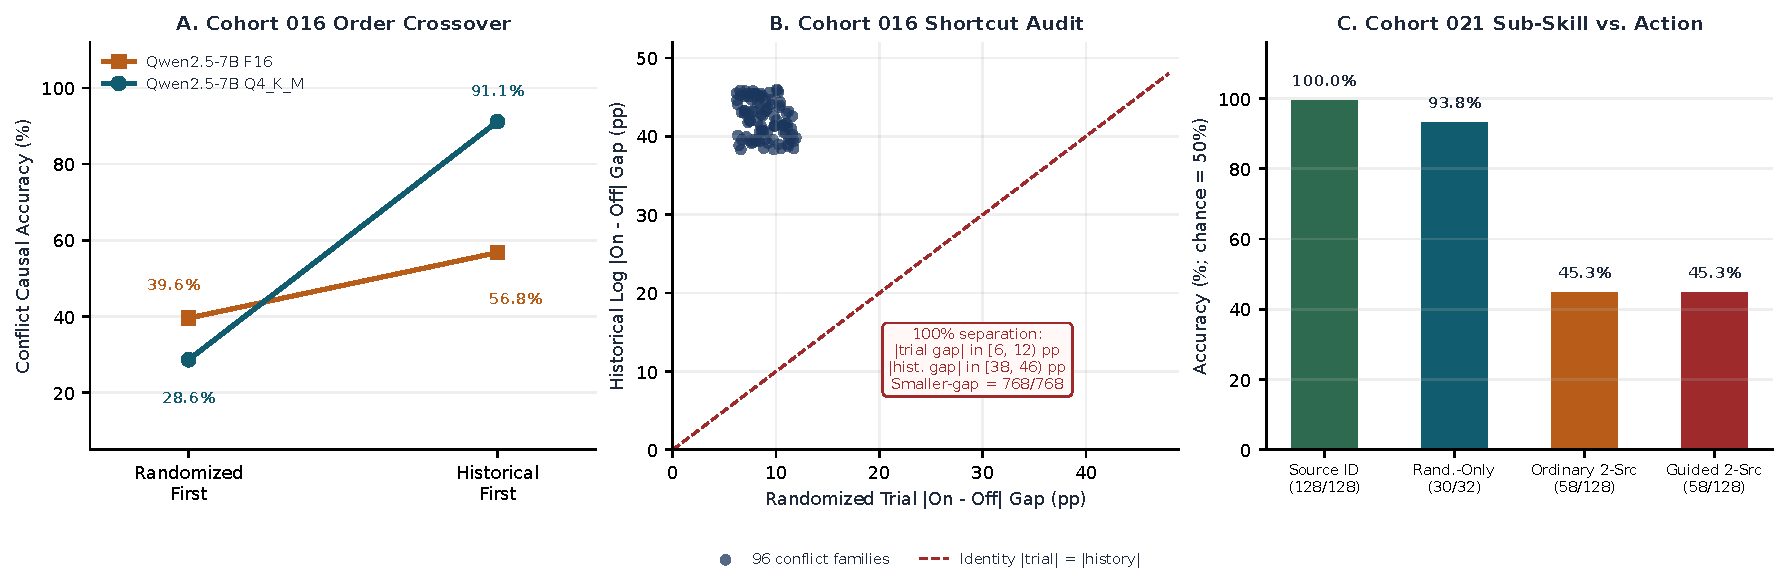
\includegraphics[width=\textwidth]{figures/fig09_evidence_selection_and_shortcut.pdf}
  \caption{The Cohort~016 order confirmation, its retrospective shortcut counterexample, and Cohort~021's component dissociation: (A) Cohort~016 96-family conflict accuracy by presentation order for \texttt{Qwen2.5-7B F16} and \texttt{Q4\_K\_M}; (B) Retrospective source-blind separation showing $|\text{trial gap}| \in [6,12)\pp < |\text{history gap}| \in [38,46)\pp$ on $100\%$ of items; (C) Cohort~021 governing-source recognition ($100\%$) vs.\ two-source decision failure ($45.3\%$).}
  \label{fig:shortcut_c16}
\end{figure}

% =============================================================================
\section{Cohort 013: Minimal vs.\ Causal-Context Prompt Crossover (160-Token Post-JSON Verbosity Failure)}

\subsection*{1. Historical Context}
Cohort~012 failed because minimal study labels (\emph{``Historical data where operators chose...''}) did not cue \texttt{Qwen2.5-7B F16} to discount confounding. Cohort~013 crossed that minimal prompt against a richer \emph{causal-context} prompt explicitly explaining that unmeasured initial severity affects both historical operator choices and outcomes.

\subsection*{2. Research Question}
Does adding explicit causal-confounding context allow \texttt{Qwen2.5-7B F16} to pass the two-study conflict reference gate?

\subsection*{3. Hypothesis}
\textbf{Classification:} \emph{Exploratory prompt-clarity crossover.} Expected causal-context prose to raise conflict accuracy above $\ge 9/16$ per order.

\subsection*{4. Experimental Design}
Single model (\texttt{Qwen2.5-7B F16}) on $8$ fresh matched-strength families (\texttt{seed=20261116}) $\times 4$ cells $\times 2$ orders $\times 2$ prompt frames (\texttt{minimal} vs.\ \texttt{causal\_context}) $= 128$ prompts (\texttt{max\_tokens=160}).

\subsection*{5. Mathematical Formulation}
Identical matched-strength two-study causal contrast (\texttt{M06}), paired within family across prompt frames.

\subsection*{6. Experimental Execution}
Completed November 12, 2026 (commit \texttt{0f55a79}). An unexpected formatting failure occurred on $64/64$ causal-context items!

\subsection*{7. Results}
\begin{itemize}
  \item \textbf{Minimal Frame:} $64/64$ single-fence valid ($0/64$ bare JSON); scored \textbf{$48/64$ ($75.0\%$)\textbf{ overall ($32/32$ aligned, }$8/16$} and \textbf{$8/16$} conflict---again failing the $\ge 9/16$ conflict gate).
  \item \textbf{Causal-Context Frame:} \textbf{$0/64$ valid} under both strict bare JSON \emph{and} single-fence parsing! Because the prompt mentioned causal reasoning concepts, \texttt{Qwen2.5-7B F16} emitted a valid fenced JSON object first and then \emph{appended a multi-sentence causal explanation afterward}, running straight into the $160$-token cap on all $64$ items! A post-hoc prefix diagnostic extracting the leading JSON scored $45/64$, which was properly refused for gate qualification.
\end{itemize}

\subsection*{8. Interpretation at the Time}
Prompting LLMs about confounding triggers didactic post-JSON explanations unless the output contract explicitly forbids Markdown fences and trailing text.

\subsection*{9. Retrospective Interpretation}
This failure directly catalyzed CausalFade's transition to strict bare-JSON contracts (\emph{``Do not include a Markdown fence, explanation, or any other text''}), raising strict bare-JSON validity from $0\%$ (Cohorts~001--013) to \textbf{$100\%$} across Cohorts~014--023 and 029!

\subsection*{10. Methodological Limitations}
Post-JSON verbosity invalidated the causal-context arm; 8-family development size.

\subsection*{11. Scientific Contribution}
\emph{Infrastructure discovery:} Identified explanation-triggering prompt spillover and motivated strict bare-JSON negative constraints.

\subsection*{12. Transition to Subsequent Research}
Cohort~014 tightened the output instruction and lowered \texttt{max\_tokens} to $48$ on $8$ fresh families.

\subsection*{13. Evidence and Reproducibility}
Artifacts: \texttt{experiments/cohort\_013/summary.md}, \texttt{run\_001\_7b\_f16/}; commit \texttt{0f55a79}.

% =============================================================================
\section{Cohort 014: Strict Bare-JSON Contract Screen (48-Token Cap)}

\subsection*{1. Historical Context}
Cohort~014 immediately tested a hardened strict-JSON output instruction (\texttt{max\_tokens=48}) across both minimal and causal-context frames on fresh families.

\subsection*{2. Research Question}
Does an explicit bare-JSON anti-fence instruction achieve $\ge 95\%$ strict JSON validity on \texttt{Qwen2.5-7B F16}, and does either frame clear the reference competence gate?

\subsection*{3. Hypothesis}
\textbf{Classification:} \emph{Documented prospective feasibility gate.} Pre-declared gate: strict bare-JSON validity $\ge 56/64$, overall accuracy $\ge 44/64$ ($68.75\%$), and conflict accuracy $\ge 9/16$ in each presentation order.

\subsection*{4. Experimental Design}
\texttt{Qwen2.5-7B F16} on $8$ fresh matched-strength families (\texttt{seed=20261119}), $64$ minimal + $64$ causal-context prompts $= 128$ requests (\texttt{max\_tokens=48}, \texttt{temperature=0.0}).

\subsection*{5. Mathematical Formulation}
Identical matched-strength two-study contrast (\texttt{M06}) scored under exact \texttt{json.loads} without fence stripping.

\subsection*{6. Experimental Execution}
Completed November 12, 2026 (commit \texttt{baa573b}). Verbatim output on every single item: \texttt{\{"activate": 1\}} or \texttt{\{"activate": 0\}}.

\subsection*{7. Results}
\begin{itemize}
  \item \textbf{Strict Bare-JSON Validity Solved:} \textbf{$128/128$ ($100.0\%$)} strict bare-JSON compliance with normal stops!
  \item \textbf{Near-Miss Gate Outcome:}
    \begin{itemize}
      \item \texttt{Minimal}: $48/64$ overall (passed $\ge 44$), $32/32$ aligned, but \textbf{$8/16$} and \textbf{$8/16$} conflict (\textbf{failed} $\ge 9/16$ conflict gate).
      \item \texttt{Causal-context}: \textbf{$9/16$ ($56.25\%$)} randomized-first conflict and \textbf{$9/16$ ($56.25\%$)} historical-first conflict (\textbf{passed} both conflict gates!), plus $24/32$ aligned, totaling \textbf{$42/64$ ($65.63\%$)} overall---missing the $\ge 44/64$ overall threshold by just $2$ items!
    \end{itemize}
\end{itemize}

\subsection*{8. Interpretation at the Time}
Strict bare JSON worked flawlessly ($128/128$), and causal-context framing cleared per-order conflict thresholds for the first time in the project, missing the overall 8-family gate by $2$ items under high discrete binomial noise.

\subsection*{9. Retrospective Interpretation}
Notice a subtle sign of trouble that would soon grow: adding causal context lowered \emph{aligned} accuracy from $32/32$ to $24/32$ ($75\%$), showing that causal-context prose perturbed aligned choices even when both studies agreed!

\subsection*{10. Methodological Limitations}
Underpowered $8$-family ($16$-item per conflict order) discrete threshold; unacknowledged $|\tau| < |\RD_{\mathrm{obs}}|$ gap invariant.

\subsection*{11. Scientific Contribution}
\emph{Infrastructure breakthrough ($100\%$ strict bare-JSON compliance) \& narrow reference-gate diagnostic.}

\subsection*{12. Transition to Subsequent Research}
Cohort~015 doubled the sample size to $16$ fresh families ($128$ causal-context prompts) with scaled pre-declared gate thresholds ($\ge 88/128$ overall, $\ge 18/32$ per conflict order) and conditional authorization to run \texttt{7B Q4\_K\_M} if \texttt{F16} passed.

\subsection*{13. Evidence and Reproducibility}
Artifacts: \texttt{experiments/cohort\_014/summary.md}, \texttt{run\_001\_7b\_f16/}; commit \texttt{baa573b}.

% =============================================================================
\section{Cohort 015: 16-Family Causal-Context Gate Pass and Discovery of the \texttt{7B Q4\_K\_M} Order Jump}

\subsection*{1. Historical Context}
Cohort~015 executed the scaled 16-family causal-context gate on \texttt{Qwen2.5-7B F16}, with a frozen plan (\texttt{frozen\_run\_plan.json}) authorizing \texttt{Qwen2.5-7B Q4\_K\_M} \emph{if and only if} \texttt{F16} cleared every threshold.

\subsection*{2. Research Question}
Does \texttt{Qwen2.5-7B F16} clear the 16-family causal-context competence gate, and if triggered, how does \texttt{7B Q4\_K\_M} compare across aligned, conflict, and study-order conditions?

\subsection*{3. Hypothesis}
\textbf{Classification:} \emph{Documented prospective gate + conditional exploratory format comparison (\texttt{H01}, \texttt{H06}).}

\subsection*{4. Experimental Design}
\texttt{Qwen2.5-7B} \texttt{F16} (\texttt{run\_001\_7b\_f16}) and conditionally triggered \texttt{Q4\_K\_M} (\texttt{run\_002\_7b\_q4\_k\_m}) on $16$ fresh matched-strength families (\texttt{seed=20261122}), $128$ strict-JSON prompts/arm ($256$ total requests).

\subsection*{5. Mathematical Formulation}
Paired 16-family comparisons on overall accuracy, conflict penalty, and within-family order contrast $\Delta_{\mathrm{order}}(p) = \mathrm{Acc}_{\mathrm{conflict}}(\mathrm{hist\text{-}first}, p) - \mathrm{Acc}_{\mathrm{conflict}}(\mathrm{rand\text{-}first}, p)$.

\subsection*{6. Experimental Execution}
Completed November 12, 2026 (commit \texttt{79c0ba5}); $256/256$ strict-valid bare JSON responses.

\subsection*{7. Results}
\emph{(From \texttt{experiments/cohort\_015/summary.md}.)}
\begin{itemize}
  \item \textbf{\texttt{7B F16} Cleared All Gate Thresholds:} $128/128$ valid ($\ge 112$), \textbf{$89/128$ ($69.53\%$)} overall ($\ge 88$), \textbf{$19/32$ ($59.38\%$)} rand-first conflict ($\ge 18$), and \textbf{$22/32$ ($68.75\%$)} hist-first conflict ($\ge 18$), legitimately triggering \texttt{Q4\_K\_M}.
  \item \textbf{\texttt{7B Q4\_K\_M} Scored Higher Overall---With a Massive $+65.6\pp$ Conflict Order Swing:}
    \begin{itemize}
      \item Aggregate \texttt{Q4\_K\_M} scored \textbf{$98/128$ ($76.56\%$)} overall ($+7.03\pp$ above \texttt{F16}, 95\% CI $[+0.78, +12.50]\pp$), with $55/64$ aligned and $43/64$ conflict (conflict-penalty difference $+7.81\pp$, CI $[-7.81, +23.44]\pp$).
      \item Splitting by study order revealed an astonishing pattern: on conflict items, \texttt{Q4\_K\_M} scored \textbf{$11/32$ ($34.38\%$)} when randomized evidence was first vs.\ \textbf{$32/32$ ($100.00\%$)\textbf{ when historical evidence was first (}$+65.625\pp$}, CI $[+56.25, +78.13]\pp$), compared to $+9.375\pp$ on \texttt{F16} (format-by-order interaction \textbf{$+56.25\pp$}, CI $[+40.63, +71.88]\pp$)!
      \item Conversely, on \emph{aligned} items, historical-first \emph{reduced} accuracy from $32/32$ to $16/32$ ($-50.0\pp$) on \texttt{F16} and from $32/32$ to $23/32$ ($-28.1\pp$) on \texttt{Q4\_K\_M}!
    \end{itemize}
\end{itemize}

\subsection*{8. Interpretation at the Time}
The researchers resisted claiming victory from a 16-family exploratory surprise: \texttt{summary.md} explicitly classified Cohort~015 as development data and pre-registered a dedicated $96$-family prospective replication of the \texttt{Q4\_K\_M} conflict-order effect in Cohort~016 (\texttt{D06}).

\subsection*{9. Retrospective Interpretation}
Look at \texttt{Q4\_K\_M}'s conflict split: $32/32$ ($100\%$) when randomized evidence was \emph{second} (historical first), vs.\ $11/32$ ($34.4\%$) when randomized evidence was \emph{first} (historical second). In a two-study prompt where the model strongly weights the \emph{final} numbers right above the question (recency bias \citep{liu2024lost}), placing the randomized trial second puts the right numbers in the recency slot, whereas placing the historical study second puts the misleading confounded numbers in the recency slot!

\subsection*{10. Methodological Limitations}
$16$ development families; single checkpoint lineage; aligned-item order drop ($-50\pp$ in \texttt{F16}) signaled strange prompt-order heuristics; hidden $|\tau| < |\RD_{\mathrm{obs}}|$ shortcut.

\subsection*{11. Scientific Contribution}
\emph{Exploratory discovery (\texttt{H06}):} Uncovered extreme recency/order sensitivity in \texttt{7B Q4\_K\_M} two-study conflict decisions and set up Cohort~016's prospective replication.

\subsection*{12. Transition to Subsequent Research}
Directly launched Cohort~016's frozen $96$-family ($1{,}536$-prompt) confirmatory replication.

\subsection*{13. Evidence and Reproducibility}
Artifacts: \texttt{experiments/cohort\_015/frozen\_run\_plan.json}, \texttt{summary.md}, \texttt{order\_analysis.json}; commit \texttt{79c0ba5}.

% =============================================================================
\section{Cohort 016: Prospective 96-Family Order Confirmation---and Retrospective Shortcut Counterexample}

\subsection*{1. Historical Context}
Cohort~016 was CausalFade's first large-scale, pre-frozen confirmatory experiment ($6\times$ larger than Cohort~015), designed specifically to test whether \texttt{Qwen2.5-7B Q4\_K\_M}'s conflict presentation-order effect replicated on $96$ brand-new SCM families.

\subsection*{2. Research Question}
On $96$ fresh matched-strength SCM families under a frozen protocol, does \texttt{Qwen2.5-7B Q4\_K\_M} exhibit a positive historical-first minus randomized-first accuracy difference on conflict items?

\subsection*{3. Hypothesis}
\textbf{Classification:} \emph{Documented prospective confirmatory hypothesis (\texttt{H06}, \texttt{frozen\_run\_plan.json}).} Primary pre-declared endpoint: paired 96-family $t$-test on $\Delta_{\mathrm{order}}(\text{\texttt{Q4\_K\_M}})$ over conflict items; secondary endpoint: format-by-order interaction $\Delta_{\mathrm{order}}(\text{\texttt{Q4\_K\_M}}) - \Delta_{\mathrm{order}}(\text{\texttt{F16}})$.

\subsection*{4. Experimental Design}
\begin{itemize}
  \item \textbf{Arms:} \texttt{Qwen2.5-7B-Instruct} \texttt{F16} (\texttt{run\_001\_7b\_f16}) and \texttt{Q4\_K\_M} (\texttt{run\_002\_7b\_q4\_k\_m}).
  \item \textbf{Sample:} $96$ fresh families (\texttt{seed=20261127}) $\times 4$ $(T,S)$ cells $\times 2$ study orders $= 768$ prompts/arm ($1{,}536$ total requests; $384$ conflict prompts/arm $= 192$ per order).
\end{itemize}

\subsection*{5. Mathematical Formulation}
For each family $i \in \{1,\dots,96\}$, let $d_i = \frac{1}{2}\sum_{c \in \{(1,0),(0,1)\}} \bigl(Y_{i,c,\mathrm{hist}} - Y_{i,c,\mathrm{rand}}\bigr) \in \{-1, -0.5, 0, +0.5, +1\}$, tested via one-sample two-sided Student $t$-statistic $t_{95} = \bar{d} / (s_d / \sqrt{96})$.

\subsection*{6. Experimental Execution}
Completed November 12, 2026 (commits \texttt{eb53578}, \texttt{13e8fa5}). All $1{,}536/1{,}536$ responses stopped normally and satisfied strict bare-JSON parsing (\texttt{\{"activate": 0\}} or \texttt{\{"activate": 1\}}).

\subsection*{7. Results}
\emph{(Distinguishing contemporaneous confirmatory statistics in \texttt{primary\_analysis.json} from the retrospective shortcut audit in \texttt{manuscript/scripts/extract.py}; see Figure~\ref{fig:shortcut_c16}A--B.)}
\begin{itemize}
  \item \textbf{Contemporaneous Confirmatory Result:}
    \begin{itemize}
      \item \texttt{7B Q4\_K\_M} conflict accuracy jumped from \textbf{$55/192$ ($28.65\%$)} randomized-first to \textbf{$175/192$ ($91.15\%$)\textbf{ historical-first: }$\bar{d} = +0.6250$ ($+62.50\pp$)}, family SD $s_d = 0.2902$, \textbf{$t(95) = 21.10$, $p = 1.24 \times 10^{-37}$}, 95\% CI $[+56.62, +68.38]\pp$!
      \item \texttt{7B F16} conflict accuracy rose from \textbf{$109/192$ ($56.77\%$)} randomized-first to \textbf{$143/192$ ($74.48\%$)} historical-first ($+17.71\pp$), yielding a secondary \texttt{Q4\_K\_M}-minus-\texttt{F16} order-sensitivity amplification of \textbf{$+44.79\pp$}!
      \item Overall accuracy: \texttt{F16} $540/768$ ($70.31\%$); \texttt{Q4\_K\_M} $577/768$ ($75.13\%$). Again, aligned accuracy dropped when historical evidence was listed first!
    \end{itemize}
  \item \textbf{Retrospective Shortcut Audit (Calculated Later in \texttt{manuscript/scripts/extract.py}):} Across all $96$ families ($768$ prompts), every randomized study had $|\text{on}-\text{off}| = |\tau_i| \in [6.00, 12.00)\pp$, whereas every historical study had $|\text{on}-\text{off}| = |\RD_{\mathrm{obs},i}| \in [38.00, 46.00)\pp$ (Figure~\ref{fig:shortcut_c16}B). Consequently, the deterministic source-blind rule
  \begin{equation}
    h_{\mathrm{min\text{-}gap}}(\text{prompt}) = \mathbb{I}\bigl(\text{on}_{k^*} - \text{off}_{k^*} > 0\bigr), \quad k^* = \arg\min_{k \in \{1,2\}} |\text{on}_k - \text{off}_k|,
  \end{equation}
  which completely ignores the words ``randomized'' and ``historical,'' predicts the exact oracle label on \textbf{$768/768$ ($100.0\%$)} of Cohort~016 prompts!
\end{itemize}

\begin{auditcallout}[Why Both Facts Matter Together]
Notice what the retrospective shortcut discovery does---and does \emph{not}---invalidate. It \emph{does not} invalidate the within-pair order contrast ($+62.50\pp$), because both orders of a pair contain the exact same numbers in swapped line positions. What it \emph{does} invalidate is interpreting Cohort~016's high accuracy ($91.15\%$ in \texttt{Q4\_K\_M} historical-first or $74.48\%$ in \texttt{F16}) as proof of genuine causal source identification: any benchmark where a source-blind numerical heuristic achieves $100\%$ cannot certify causal provenance reasoning!
\end{auditcallout}

\subsection*{8. Interpretation at the Time}
Celebrated cautiously in \texttt{experiments/cohort\_016/summary.md} as a clean prospective replication of prompt-order amplification under 4-bit quantization on \texttt{Qwen2.5-7B}, while explicitly noting that cross-size and cross-prompt generalization remained untested.

\subsection*{9. Retrospective Interpretation}
Cohort~016 became the centerpiece cautionary tale of \texttt{manuscript/article.tex} (Figure~5 of the final paper): even a pre-frozen, 96-family, $p = 10^{-37}$ behavioral effect on a specific prompt template turned out to be (i) checkpoint- and template-fragile ($0\pp$ in Cohort~017 \texttt{14B Q4} and $0\pp$ in Cohort~024's semantic scaffold) and (ii) embedded inside a benchmark solvable $100\%$ of the time by a source-blind magnitude rule.

\subsection*{10. Methodological Limitations}
Complete disjointness of $|\tau|$ and $|\RD_{\mathrm{obs}}|$ intervals; absence of matched noncausal controls; single prompt template and single 7B checkpoint lineage.

\subsection*{11. Scientific Contribution}
\emph{Positive empirical confirmation (template-specific 7B order effect) \& landmark retrospective benchmark-artifact counterexample.}

\subsection*{12. Transition to Subsequent Research}
Prompted Cohort~017 to test whether the order interaction generalized to \texttt{Qwen2.5-14B}, and Cohorts~018--024 to add matched noncausal controls and cross-lineage checks.

\subsection*{13. Evidence and Reproducibility}
Artifacts: \texttt{experiments/cohort\_016/frozen\_run\_plan.json}, \texttt{primary\_analysis.json}, \texttt{run\_001\_7b\_f16/}, \texttt{run\_002\_7b\_q4\_k\_m/}, \texttt{manuscript/scripts/extract.py}; commits \texttt{eb53578}, \texttt{13e8fa5}.

% =============================================================================
\section{Cohort 017: Exploratory \texttt{Qwen2.5-14B} Follow-Up (and Analysis Environment Recovery)}

\subsection*{1. Historical Context}
Immediately after Cohort~016, the researchers ran an unattended overnight follow-up on \texttt{Qwen2.5-14B-Instruct} over Cohort~016's exact $768$-prompt schedule. Because \texttt{14B F16} ($\approx 29.5\;\text{GiB}$) exceeded safe $32\;\text{GiB}$ host memory margins, \texttt{14B Q8\_0} ($14.6\;\text{GiB}$) served as the high-precision comparator alongside \texttt{14B Q4\_K\_M}.

\subsection*{2. Research Question}
Does Cohort~016's massive conflict-order effect ($+62.5\pp$) generalize up the same model lineage to \texttt{Qwen2.5-14B} (\texttt{Q8\_0} and \texttt{Q4\_K\_M})?

\subsection*{3. Hypothesis}
\textbf{Classification:} \emph{Exploratory cross-scale follow-up (\texttt{H06}).}

\subsection*{4. Experimental Design}
\texttt{Qwen2.5-14B-Instruct} \texttt{Q8\_0} (\texttt{run\_001\_14b\_q8\_0}) and \texttt{Q4\_K\_M} (\texttt{run\_002\_14b\_q4\_k\_m}) on Cohort~016's $96$ families ($768$ prompts/arm, $1{,}536$ total requests).

\subsection*{5. Mathematical Formulation}
Paired 96-family order contrast $\Delta_{\mathrm{order}}$; required adding a zero-variance denominator guard ($s_d = 0 \implies t = \text{null}$) when \texttt{14B Q4\_K\_M} emitted identical constant predictions across every conflict pair!

\subsection*{6. Experimental Execution}
Both inference runs completed $768/768$ strict-valid responses overnight on November 13, 2026 (commit \texttt{40f34f8}), but the unattended post-run analyzer crashed with \texttt{ModuleNotFoundError: No module named 'numpy'} because the background shell invoked a bare system Python without \texttt{numpy}. Preserving the failure log untouched, the researchers ran recovery analysis locally under Python \texttt{3.13.5} + NumPy \texttt{2.3.5} (\texttt{analysis\_recovery.json}, commit \texttt{caf5b1d}).

\subsection*{7. Results}
\begin{itemize}
  \item \textbf{\texttt{14B Q8\_0}:} $488/768$ ($63.54\%$) overall; conflict accuracy was \textbf{$104/192$ ($54.17\%$)} randomized-first vs.\ \textbf{$96/192$ ($50.00\%$)\textbf{ historical-first (}$-4.17\pp$}, 95\% CI $[-6.98, -1.35]\pp$).
  \item \textbf{\texttt{14B Q4\_K\_M}:} $440/768$ ($57.29\%$) overall; conflict accuracy was \textbf{$96/192$ ($50.00\%$)} in \emph{both\textbf{ orders (}$0.00\pp$\textbf{ order contrast, zero family variance) because \texttt{14B Q4\_K\_M} output \texttt{"activate": 1} on }$384/384$ ($100\%$)} of conflict items!
  \item On aligned historical-first items, \emph{both} \texttt{14B} arms activated on $192/192$ items ($96/192 = 50.0\%$ accuracy vs.\ $192/192$ and $152/192$ randomized-first).
\end{itemize}

\subsection*{8. Interpretation at the Time}
Cohort~017 delivered a sobering reality check: (1) Cohort~016's $+62.5\pp$ conflict-order effect did \emph{not} generalize to \texttt{14B}; (2) doubling parameters from $7\text{B}$ to $14\text{B}$ actually \emph{lowered} overall accuracy ($70.3\% \to 63.5\%$) and collapsed conflict decisions back into $100\%$ \texttt{activate=1} bias; and (3) a $0\pp$ order contrast in \texttt{14B Q4\_K\_M} reflected total degeneracy, not ``order robustness.''

\subsection*{9. Retrospective Interpretation}
This failure to generalize across sizes within the \emph{exact same Qwen2.5 family} prevented the project from publishing a brittle single-checkpoint anomaly as a general law of quantized LLMs, launching Phase~V's deep diagnostic audit of controls, response tokens, and sub-skills.

\subsection*{10. Methodological Limitations}
Reused Cohort~016's $96$ families; \texttt{Q8\_0} substituted for \texttt{F16} due to 32 GiB RAM ceiling.

\subsection*{11. Scientific Contribution}
\emph{Negative cross-scale replication \& statistical edge-case hardening (zero-variance $t$-guard).}

\subsection*{12. Transition to Subsequent Research}
Forced a fundamental rethink in Cohorts~018--023: adding matched noncausal controls, neutral response tokens, and component skill diagnostics to find out \emph{why} models defaulted to \texttt{activate=1} whenever two studies appeared together.

\subsection*{13. Evidence and Reproducibility}
Artifacts: \texttt{experiments/cohort\_017/summary.md}, \texttt{analysis.json}, \texttt{analysis\_recovery.json}, \texttt{run\_001\_14b\_q8\_0/}, \texttt{run\_002\_14b\_q4\_k\_m/}; commits \texttt{40f34f8}, \texttt{caf5b1d}.

% =============================================================================
% Part II, Chapter 9: Cohorts 018--023
% =============================================================================
\chapter{Instruction Sensitivity, Component Decomposition, and Recognition-Action Dissociation (Cohorts 018--023)}\label{ch:cohorts_018_023}

When Cohort~017 showed that \texttt{Qwen2.5-14B} failed to reproduce \texttt{7B}'s order interaction and instead defaulted to \texttt{activate=1} across $100\%$ of conflict items, the researchers paused quantization runs altogether and spent six diagnostic cohorts (Cohorts~018--023, November 13--16, 2026) dissecting \emph{why} unquantized \texttt{F16} models behaved so erratically on two-study prompts. By introducing matched noncausal controls, reversed token polarity, neutral symbol labels (\texttt{K}/\texttt{M}), component sub-skill probes, explicit governing-source reminders, and a second model lineage (\texttt{Mistral-7B-v0.3}), this phase uncovered a striking cognitive-style dissociation in LLMs: \textbf{perfect explicit recognition of which evidence source governs an intervention ($128/128$) coupled with chance-level failure to apply that very source when choosing an action ($58/128$)}.

% =============================================================================
\section{Cohort 018: Graded-Sensitivity, Reversed-Polarity, and Matched-Control Pilot}

\subsection*{1. Historical Context}
Up through Cohort~017, every experiment lacked a matched noncausal control task on the same numerical spreads and assumed \texttt{activate=1} meant ``activate'' and \texttt{activate=0} meant ``leave off.'' Cohort~018 introduced both a matched noncausal rule-following control and an explicit polarity reversal (\texttt{activate=0} $\leftrightarrow$ \texttt{activate=1}) on \texttt{Qwen2.5-7B F16}.

\subsection*{2. Research Question}
Does \texttt{Qwen2.5-7B F16} pass causal competence gates when evaluated alongside matched noncausal rule-following controls and reversed integer-to-action polarity mappings?

\subsection*{3. Hypothesis}
\textbf{Classification:} \emph{Documented prospective development gate (\texttt{H07}, \texttt{H08}).} Required \texttt{F16} causal accuracy $\ge 80/128$ and $\ge 18/32$ per conflict order before running \texttt{Q4\_K\_M}.

\subsection*{4. Experimental Design}
Single arm (\texttt{Qwen2.5-7B F16}) on $8$ fresh families (\texttt{seed=20261114}), $288$ strict-JSON prompts crossing causal two-study items ($128$), matched noncausal rule controls ($128$, e.g., \emph{``If the FIRST study assigned X randomly, choose activate X; otherwise choose leave X off''}), and reversed integer token mappings ($32$ diagnostic items).

\subsection*{5. Mathematical Formulation}
Separates semantic action preference (\emph{activate X}) from integer token preference (\texttt{1} vs.\ \texttt{0}) by crossing action polarity $m \in \{\text{standard}, \text{reversed}\}$ against gold action $g \in \{0,1\}$.

\subsection*{6. Experimental Execution}
Completed November 13--14, 2026 (commit \texttt{00fd0b5}); $288/288$ ($100\%$) strict-valid JSON responses.

\subsection*{7. Results}
\begin{itemize}
  \item \textbf{Causal Gate Failed:} \texttt{7B F16} scored \textbf{$64/128$ ($50.00\%$)} on causal items (failing $\ge 80/128$) and \textbf{$14/32$ ($43.75\%$)} on historical-first conflict (failing $\ge 18/32$).
  \item \textbf{Matched Noncausal Control Also Failed:} On noncausal conditional instructions over the same study labels, \texttt{7B F16} scored only \textbf{$62/128$ ($48.44\%$)}!
  \item \textbf{Catastrophic Token-Polarity Fragility:} Reversing the response code so \texttt{activate=0} meant ``activate X'' collapsed accuracy from \textbf{$50/64$ ($78.13\%$)} to \textbf{$14/64$ ($21.88\%$)} ($-56.25\pp$), because the model bound the English word \texttt{activate} lexically to integer \texttt{1} regardless of explicit definitions!
\end{itemize}

\subsection*{8. Interpretation at the Time}
Per protocol, \texttt{Q4\_K\_M} was withheld. Two critical measurement confounds were diagnosed: (1) lexical entanglement between key name \texttt{"activate"} and integer \texttt{1}, and (2) baseline failure on conditional noncausal instructions ($62/128$).

\subsection*{9. Retrospective Interpretation}
Cohort~018 proved why matched noncausal controls are indispensable: without the $62/128$ control arm, $64/128$ causal accuracy would have been misdiagnosed purely as ``confounding blindness.''

\subsection*{10. Methodological Limitations}
Counter-intuitive reversed polarity (\texttt{activate=0} meaning ``activate'') created an artificial Stroop-like conflict with natural English semantics.

\subsection*{11. Scientific Contribution}
\emph{Benchmark artifact discovery:} Exposed lexical key-value binding (\texttt{"activate": 1}) and baseline conditional-rule failure.

\subsection*{12. Transition to Subsequent Research}
Motivated Cohort~019 to replace \texttt{"activate": 0/1} with neutral symbolic contracts (\texttt{\{"choice": "K"\}} vs.\ \texttt{"M"}).

\subsection*{13. Evidence and Reproducibility}
Artifacts: \texttt{experiments/cohort\_018/summary.md}, \texttt{run\_001\_7b\_f16/}; commit \texttt{00fd0b5}.

% =============================================================================
\section{Cohort 019: Within-World Response-Contract Crossover (\texttt{K}/\texttt{M} vs.\ Semantic)}

\subsection*{1. Historical Context}
To test whether removing the loaded word \texttt{"activate"} from the JSON schema restored causal performance, Cohort~019 compared semantic labels against neutral arbitrary letter codes (\texttt{"choice": "K"} vs.\ \texttt{"choice": "M"}) crossed in forward and reverse action assignments on the exact same worlds.

\subsection*{2. Research Question}
Do neutral symbolic output contracts (\texttt{K}/\texttt{M}) eliminate response-label bias and allow \texttt{Qwen2.5-7B F16} to pass causal and comprehension gates?

\subsection*{3. Hypothesis}
\textbf{Classification:} \emph{Documented prospective development gate (\texttt{H07}).}

\subsection*{4. Experimental Design}
Single arm (\texttt{Qwen2.5-7B F16}) on $8$ fresh 6-decimal probability families (\texttt{seed=20261115}), \textbf{$832$ prompts} crossing semantic, neutral-forward (\texttt{K}=off, \texttt{M}=on), and neutral-reverse (\texttt{K}=on, \texttt{M}=off) contracts across causal tasks, noncausal controls, and study comprehension checks.

\subsection*{5. Mathematical Formulation}
Within-world invariance requires $\hat{a}_{\mathrm{semantic}}(w) = \hat{a}_{\mathrm{neu\text{-}fwd}}(w) = \hat{a}_{\mathrm{neu\text{-}rev}}(w)$ for identical underlying decision worlds $w$.

\subsection*{6. Experimental Execution}
Completed November 14, 2026 (commit \texttt{a400569}); \textbf{$832/832$ ($100.0\%$)} strict-valid JSON responses (\texttt{\{"choice":"M"\}}).

\subsection*{7. Results}
\begin{itemize}
  \item \textbf{Semantic Gate Failed:} Semantic causal accuracy was \textbf{$73/128$ ($57.03\%$)}, with conflict accuracy \textbf{$12/32$ ($37.5\%$)\textbf{ and }$13/32$ ($40.6\%$)}, and study comprehension $24/32$ ($75.0\%$).
  \item \textbf{Neutral Letters Introduced Strong Alphabetical/Position Asymmetry:} Neutral-reverse (\texttt{K}=activate) outperformed neutral-forward (\texttt{K}=leave\_off) by \textbf{$+25.78\pp$} on causal items and \textbf{$+36.72\pp$} on noncausal controls because the model favored letter \texttt{"K"} (the first-defined code in the prompt), aiding activation when \texttt{K}=on and hurting it when \texttt{K}=off!
  \item \textbf{Self-Audited Prompt Bug:} Contemporaneous inspection in \texttt{summary.md} transparently documented a minor wording bug in one comprehension check cue and withheld \texttt{Q4\_K\_M}.
\end{itemize}

\subsection*{8. Interpretation at the Time}
Arbitrary letter codes (\texttt{K}/\texttt{M}) traded semantic \texttt{activate} bias for strong first-defined-symbol bias ($+25.8\pp$ to $+36.7\pp$), failing measurement invariance \citep{lohn2024machinepsychology}.

\subsection*{9. Retrospective Interpretation}
Proved that prompt-level symbol neutralization is not a silver bullet; instead, benchmarks must counterbalance option order and score paired transitions across invariant and switching worlds (as ultimately realized in Cohorts~027 and 029).

\subsection*{10. Methodological Limitations}
Comprehension-probe wording bug (documented contemporaneously); single 7B F16 checkpoint.

\subsection*{11. Scientific Contribution}
\emph{Benchmark artifact discovery:} Demonstrated $+25.8\pp$ to $+36.7\pp$ symbolic mapping non-invariance under neutral letter codes.

\subsection*{12. Transition to Subsequent Research}
Instead of guessing at surface response codes, Cohort~020 decomposed the two-study causal task into four atomic cognitive sub-steps to see exactly where the pipeline broke down.

\subsection*{13. Evidence and Reproducibility}
Artifacts: \texttt{experiments/cohort\_019/frozen\_run\_plan.json}, \texttt{summary.md}, \texttt{run\_001\_7b\_f16/}; commit \texttt{a400569}.

% =============================================================================
\section{Cohort 020: Staged Component Sub-Skill Diagnostic}

\subsection*{1. Historical Context}
Why did \texttt{Qwen2.5-7B F16} repeatedly score near $40\%$--$57\%$ on two-study causal prompts? Four distinct hypotheses competed: (a) inability to compare 6-decimal numbers, (b) inability to make an interventional decision from a single randomized trial, (c) inability to identify which study is randomized vs.\ historical, or (d) interference when both studies appear together. Cohort~020 tested all four stages separately on the exact same worlds!

\subsection*{2. Research Question}
Which component sub-skill fails in \texttt{Qwen2.5-7B F16}: decimal reading, single-source randomized action selection, governing-source identification, or two-source integration?

\subsection*{3. Hypothesis}
\textbf{Classification:} \emph{Exploratory component decomposition (\texttt{H09}).}

\subsection*{4. Experimental Design}
Single arm (\texttt{Qwen2.5-7B F16}) on $8$ fresh families (\texttt{seed=20261116}), \textbf{$224$ prompts} using explicit string decisions (\texttt{\{"decision": "activate"\}} vs.\ \texttt{"leave\_off"}) across four sub-tasks: (1) bare two-number comparison ($32$), (2) randomized-study-only intervention decision ($32$), (3) direct source-reliability identification ($32$), and (4) full two-study decisions ($128$).

\subsection*{5. Mathematical Formulation}
Let $p_{\mathrm{num}}, p_{\mathrm{rct}}, p_{\mathrm{id}}$ denote component accuracies; under serial independent execution without distractor interference, two-source conflict accuracy should approach $p_{\mathrm{id}} \cdot p_{\mathrm{rct}}$.

\subsection*{6. Experimental Execution}
Completed November 14, 2026 (commit \texttt{737c945}); \textbf{$224/224$ ($100.0\%$)} strict-valid JSON responses.

\subsection*{7. Results}
\begin{itemize}
  \item \textbf{Every Isolated Component Succeeded:}
    \begin{itemize}
      \item Bare 6-decimal comparison: \textbf{$28/32$ ($87.50\%$)}.
      \item Single-source randomized-only causal decision: \textbf{$29/32$ ($90.63\%$)}.
      \item Direct governing-source identification (\emph{which study identifies causal effect?}): \textbf{$32/32$ ($100.00\%$)}!
    \end{itemize}
  \item \textbf{Two-Source Integration Collapsed Under Interference:} Adding the confounded historical study alongside the exact same randomized study dropped historical-first conflict accuracy to \textbf{$16/32$ ($50.00\%$)}, with the model outputting \texttt{"leave\_off"\textbf{ on }$32/32$ ($100\%$)} of those items ($0/32$ \texttt{activate})---dramatically violating $p_{\mathrm{id}}\cdot p_{\mathrm{rct}} = 1.00 \times 0.906 = 90.6\%$!
\end{itemize}

\subsection*{8. Interpretation at the Time}
Pinpointed the bottleneck cleanly: \texttt{Qwen2.5-7B F16} possesses all three elementary ingredients (decimal comparison, single-RCT decision-making, and $100\%$ declarative recognition that randomized assignment governs intervention), yet suffers catastrophic \textbf{two-source distractor interference} when confounded historical numbers sit in the same prompt.

\subsection*{9. Retrospective Interpretation}
This was a major conceptual breakthrough in CausalFade, shifting the project's understanding from ``missing causal knowledge'' to \textbf{execution/integration failure under competing numerical cues} \citep{chen2026acedbench,zhang2026epistemic}.

\subsection*{10. Methodological Limitations}
$8$-family sample; did not yet test whether explicitly instructing the model in the prompt to \emph{use only the governing source} would fix the two-source collapse.

\subsection*{11. Scientific Contribution}
\emph{Positive diagnostic discovery (\texttt{H09}):} Isolated two-source interference from intact component skills ($32/32$ source ID, $29/32$ single-RCT).

\subsection*{12. Transition to Subsequent Research}
Directly inspired Cohort~021: if the model knows which source governs ($100\%$), what happens when we explicitly remind it to focus on the governing causal source right before deciding?

\subsection*{13. Evidence and Reproducibility}
Artifacts: \texttt{experiments/cohort\_020/frozen\_run\_plan.json}, \texttt{summary.md}, \texttt{run\_001\_7b\_f16/}; commit \texttt{737c945}.

% =============================================================================
\section{Cohort 021: Governing-Source Selection vs.\ Source-Guided Action Dissociation}

\subsection*{1. Historical Context}
Cohort~020 left one obvious question open: perhaps in an unguided two-source prompt, \texttt{Qwen2.5-7B F16} simply forgets to check assignment method before comparing numbers. Cohort~021 tested explicit \emph{source-guided} prompts reminding the model to identify the causally valid study and base its decision solely on that study.

\subsection*{2. Research Question}
Does explicit in-prompt causal-source guidance rescue \texttt{Qwen2.5-7B F16}'s two-source intervention decisions?

\subsection*{3. Hypothesis}
\textbf{Classification:} \emph{Exploratory guidance intervention (\texttt{H09}).} Expected source-guided prompting to bridge the gap between $100\%$ source identification and $50\%$ two-source action accuracy.

\subsection*{4. Experimental Design}
Single arm (\texttt{Qwen2.5-7B F16}) on $8$ fresh families (\texttt{seed=20261117}), \textbf{$576$ strict-JSON prompts} comparing: (1) randomized-only decisions ($32$), (2) governing-source selection across all $128$ two-source layouts ($128$), (3) ordinary two-source decisions ($128$), (4) explicitly source-guided two-source decisions ($128$), and (5) neutral-guided controls ($160$).

\subsection*{5. Mathematical Formulation}
Paired within-item McNemar/sign contrast between ordinary decision $Y_{j,\mathrm{ord}}$ and source-guided decision $Y_{j,\mathrm{guided}}$ across $j=1,\dots,128$ items.

\subsection*{6. Experimental Execution}
Completed November 14, 2026 (commit \texttt{77361f5}); \textbf{$576/576$ ($100.0\%$)} strict-valid JSON responses.

\subsection*{7. Results}
\emph{(Displayed in Figure~\ref{fig:shortcut_c16}C; from \texttt{experiments/cohort\_021/summary.md}.)}
\begin{itemize}
  \item \textbf{Governing-Source Selection:} \textbf{$128/128$ ($100.00\%$)}! Across every study label (\texttt{A}/\texttt{B}) and physical order, \texttt{7B F16} named the randomized study without a single error.
  \item \textbf{Single-Source Randomized-Only Decisions:} \textbf{$30/32$ ($93.75\%$)}.
  \item \textbf{Zero Rescue From Source Guidance:} Ordinary two-source decisions scored \textbf{$58/128$ ($45.31\%$)}---and explicitly source-guided two-source decisions scored \textbf{$58/128$ ($45.31\%$)} ($\widehat{\Delta} = 0.00\pp$, with exactly $11$ items improving and $11$ items worsening)!
\end{itemize}

\subsection*{8. Interpretation at the Time}
Established a stark \textbf{recognition-vs.-action dissociation}: in a single forward pass without externalized intermediate state, \texttt{Qwen2.5-7B F16} cannot bind its $100\%$-accurate source-identification capability to selective numerical lookup when distractor rates are co-present in context.

\subsection*{9. Retrospective Interpretation}
Cohort~021 explains why purely verbal prompt engineering (\emph{``pay attention to the randomized study''}) repeatedly failed throughout CausalFade, foreshadowing Cohort~028's finding that single-pass LLMs struggle whenever rule selection and numerical aggregation must compose in-context.

\subsection*{10. Methodological Limitations}
Evaluated single-turn JSON output (\texttt{max\_tokens=48}) without multi-turn source extraction; restricted to \texttt{Qwen2.5-7B F16}.

\subsection*{11. Scientific Contribution}
\emph{Landmark negative/diagnostic finding (\texttt{H09}):} Proved $0.00\pp$ gain ($58/128$ vs.\ $58/128$) from explicit source guidance despite $128/128$ governing-source recognition.

\subsection*{12. Transition to Subsequent Research}
Raised an urgent external-validity question: was this component-strong / two-source-weak profile unique to \texttt{Qwen2.5}, or shared by an independent model lineage? Cohort~022 introduced \texttt{Mistral-7B-Instruct-v0.3}.

\subsection*{13. Evidence and Reproducibility}
Artifacts: \texttt{experiments/cohort\_021/frozen\_run\_plan.json}, \texttt{summary.md}, \texttt{run\_001\_7b\_f16/}; commit \texttt{77361f5}.

% =============================================================================
\section{Cohort 022: Cross-Lineage Replication (\texttt{Qwen2.5-7B F16} vs.\ \texttt{Mistral-7B-v0.3 Q4\_K\_M})}

\subsection*{1. Historical Context}
Every experiment from Cohort~001 to Cohort~021 had queried Alibaba's \texttt{Qwen2.5} family. On November 16, 2026, Cohort~022 onboarded an independent European open-weight lineage, \texttt{Mistral-7B-Instruct-v0.3} (initially available locally as \texttt{Q4\_K\_M}), alongside \texttt{Qwen2.5-7B F16} on $8$ fresh worlds.

\subsection*{2. Research Question}
Does Cohort~021's $+48\pp$ gap between single-source randomized competence and two-source decisions replicate on fresh worlds in \texttt{Qwen2.5-7B F16}, and how does \texttt{Mistral-7B-v0.3 Q4\_K\_M} perform on the same component battery?

\subsection*{3. Hypothesis}
\textbf{Classification:} \emph{Exploratory cross-lineage development screen (\texttt{H09}, \texttt{H10}).}

\subsection*{4. Experimental Design}
Two arms (\texttt{run\_001\_qwen\_f16} and \texttt{run\_002\_mistral\_q4}) on $8$ fresh families (\texttt{seed=20261118}), \textbf{$576$ prompts/arm} ($1{,}152$ total requests) matching Cohort~021's component-and-two-source battery.

\subsection*{5. Mathematical Formulation}
Within-lineage component-minus-composite gap $\Delta_{\mathrm{comp}} = \mathrm{Acc}_{\mathrm{rct\text{-}only}} - \mathrm{Acc}_{\mathrm{two\text{-}source}}$, plus label-bias diagnostics across \texttt{Study A} vs.\ \texttt{Study B}.

\subsection*{6. Experimental Execution}
Completed November 16, 2026 (commit \texttt{21dabb2}); \textbf{$1{,}152/1{,}152$ ($100.0\%$)} strict-valid JSON responses (note \texttt{Mistral} emitted a leading space \texttt{' \{"decision":"activate"\}'}, valid under standard JSON whitespace rules).

\subsection*{7. Results}
\begin{itemize}
  \item \textbf{\texttt{Qwen2.5-7B F16} Replicated Cohort~021 Precisely:} Governing-source selection \textbf{$128/128$ ($100.0\%$)}, single-source randomized-only \textbf{$31/32$ ($96.88\%$)\textbf{, vs.\ ordinary two-source decisions }$56/128$ ($43.75\%$)\textbf{---repeating a }$+53.13\pp$} single-to-two-source collapse!
  \item \textbf{\texttt{Mistral-7B-v0.3 Q4\_K\_M} Failed Elementary Components via Pure Label Bias:} Governing-source selection was \textbf{$64/128$ ($50.00\%$)} because Mistral answered \texttt{"Study A"\textbf{ on }$128/128$ items\textbf{! Single-source randomized-only accuracy was }$16/32$ ($50.00\%$)\textbf{ because Mistral answered \texttt{"activate"} on }$32/32$ items}!
\end{itemize}

\subsection*{8. Interpretation at the Time}
Confirmed that \texttt{Qwen2.5-7B F16}'s component-vs.-integration dissociation was highly reproducible across fresh worlds, while revealing that \texttt{Mistral-7B Q4\_K\_M} failed basic first-label/first-option component checks---though because Mistral was tested at \texttt{Q4\_K\_M} rather than \texttt{F16}, Cohort~024 would soon need all 7 formats including \texttt{Mistral F16} to separate lineage behavior from quantization!

\subsection*{9. Retrospective Interpretation}
Mistral's $128/128$ \texttt{"Study A"} selection in Cohort~022 was the earliest warning of what Cohort~024 and Cohort~025 later proved on \texttt{Mistral F16}: a rigid \textbf{first-listed-option policy} ($256/256$ first option).

\subsection*{10. Methodological Limitations}
Crossed lineage with precision (\texttt{Qwen F16} vs.\ \texttt{Mistral Q4\_K\_M}) in this preliminary screen; resolved in Cohort~024's full $3\times 7$ matrix.

\subsection*{11. Scientific Contribution}
\emph{Positive within-Qwen replication ($+53.1\pp$ gap) \& cross-lineage position/label bias discovery.}

\subsection*{12. Transition to Subsequent Research}
Before launching the full multi-lineage quantization matrix, Cohort~023 audited whether \texttt{Qwen2.5-7B F16}'s component controls themselves survived full counterbalancing of source names, physical order, and option order---including \emph{harmful-direction} ($g=0$) splits!

\subsection*{13. Evidence and Reproducibility}
Artifacts: \texttt{experiments/cohort\_022/frozen\_run\_plan.json}, \texttt{summary.md}, \texttt{run\_001\_qwen\_f16/}, \texttt{run\_002\_mistral\_q4/}; commit \texttt{21dabb2}.

% =============================================================================
\section{Cohort 023: Fully Counterbalanced Measurement Audit (Discovery of Harmful-Direction Control Failure)}

\subsection*{1. Historical Context}
In Cohorts~020--022, aggregate component accuracy ($28/32$ to $31/32$) looked reassuringly high ($\ge 87.5\%$). However, if a model has a strong \texttt{activate} bias, it can score $16/16$ ($100\%$) when the true answer is \texttt{activate} and $12/16$ ($75\%$) when the true answer is \texttt{leave\_off}, hiding directional fragility inside an $87.5\%$ average! Cohort~023 crossed source name (\texttt{A}/\texttt{B}), physical study order, and listed option order, and enforced a strict \textbf{directional $\ge 75\%$ robustness rule} on both beneficial ($g=1$) and harmful ($g=0$) controls.

\subsection*{2. Research Question}
Does \texttt{Qwen2.5-7B F16} pass $\ge 75\%$ accuracy in \emph{every directional cell} (especially harmful $g=0$ cells) on bare numeric and matched noncausal scorecard controls?

\subsection*{3. Hypothesis}
\textbf{Classification:} \emph{Documented prospective measurement audit (\texttt{H08}, \texttt{H10}).}

\subsection*{4. Experimental Design}
Single arm (\texttt{Qwen2.5-7B F16}) on $8$ fresh families (\texttt{seed=20261119}), \textbf{$896$ strict-JSON prompts} crossing study names (\texttt{A}/\texttt{B}), physical order, and option display order across randomized-only ($64$), source selection ($256$), two-source causal ($256$), two-source noncausal scorecard controls ($256$), and bare numeric comparisons ($64$).

\subsection*{5. Mathematical Formulation}
Directional robustness requires $\min_{g \in \{0,1\}} \mathrm{Acc}(\text{control} \mid G=g) \ge 0.75$ rather than merely $\frac{1}{2}[\mathrm{Acc}(G=1) + \mathrm{Acc}(G=0)] \ge 0.75$.

\subsection*{6. Experimental Execution}
Completed November 16, 2026 (commit \texttt{4aff668}); \textbf{$896/896$ ($100.0\%$)} strict-valid JSON responses.

\subsection*{7. Results}
\begin{itemize}
  \item \textbf{Simple Single-Source Components Held Up:} Randomized-only causal decisions scored \textbf{$64/64$ ($100.0\%$)} and governing-source selection scored \textbf{$244/256$ ($95.31\%$)\textbf{, while two-source causal decisions dropped by }$-55.47\pp$} ($114/256 = 44.53\%$) regardless of study name or option order.
  \item \textbf{Harmful-Direction Controls Failed the $\ge 75\%$ Gate:}
    \begin{itemize}
      \item On bare numeric comparison when leaving $X$ off was larger ($g=0$), accuracy fell to \textbf{$18/32$ ($56.25\% < 75\%$)}!
      \item On matched two-source noncausal scorecard controls when leaving $X$ off won ($g=0$), accuracy fell to \textbf{$75/128$ ($58.59\% < 75\%$)}!
    \end{itemize}
\end{itemize}

\subsection*{8. Interpretation at the Time}
A crucial methodological discovery: even when causal language was removed in matched two-source noncausal controls, \texttt{Qwen2.5-7B F16} failed harmful-direction ($g=0$) decisions ($58.6\%$), proving that part of the two-source deficit was \textbf{noncausal multi-table distractor/direction bias} rather than uniquely causal confounding vulnerability!

\subsection*{9. Retrospective Interpretation}
Cohort~023 established the directional diagnostic standard (\texttt{Gold Off} vs.\ \texttt{Gold On}) that later proved decisive in Cohort~024 and Cohort~029 (where \texttt{Gold Off} causal transfer accuracy collapsed to $14/512 = 2.73\%$).

\subsection*{10. Methodological Limitations}
Single model (\texttt{Qwen2.5-7B F16}); $8$ families.

\subsection*{11. Scientific Contribution}
\emph{Methodological \& diagnostic breakthrough:} Uncovered directional ($g=0$) failure on noncausal controls ($58.6\%$), preventing false attribution of general two-table bias to causal reasoning alone.

\subsection*{12. Transition to Subsequent Research}
Set the stage for CausalFade's largest empirical campaign: Cohort~024's $30{,}912$-request cross-lineage quantization matrix across three model families and seven GGUF formats.

\subsection*{13. Evidence and Reproducibility}
Artifacts: \texttt{experiments/cohort\_023/frozen\_run\_plan.json}, \texttt{summary.md}, \texttt{run\_001\_qwen\_f16/}; commit \texttt{4aff668}.

% =============================================================================
% Part II, Chapter 10: Cohorts 024, 025, and 025.1
% =============================================================================
\chapter{The 21-Arm Cross-Lineage Quantization Matrix and Archive Re-Audits (Cohorts 024, 025, and 025.1)}\label{ch:cohorts_024_025}

Between November 16 and November 19, 2026, Project CausalFade executed its largest multi-model quantization study---Cohort~024, comprising \textbf{$30{,}912$ scheduled LLM inference requests} ($64.1\%$ of all LLM calls in the entire project!) across three independent 7B--8B transformer lineages and all seven standard GGUF precision tiers---followed by two zero-inference cross-cohort mathematical audits (Cohorts~025 and 025.1). If post-training quantization selectively degraded causal confounding resistance relative to matched noncausal controls across open-weight instruction models, Cohort~024 was engineered to see it. Instead, Cohort~024 delivered a sweeping empirical refutation of naive cross-precision causal benchmarking (Figure~\ref{fig:c24_matrix} and Table~\ref{tab:c24_matrix}).

\begin{figure}[htbp]
  \centering
  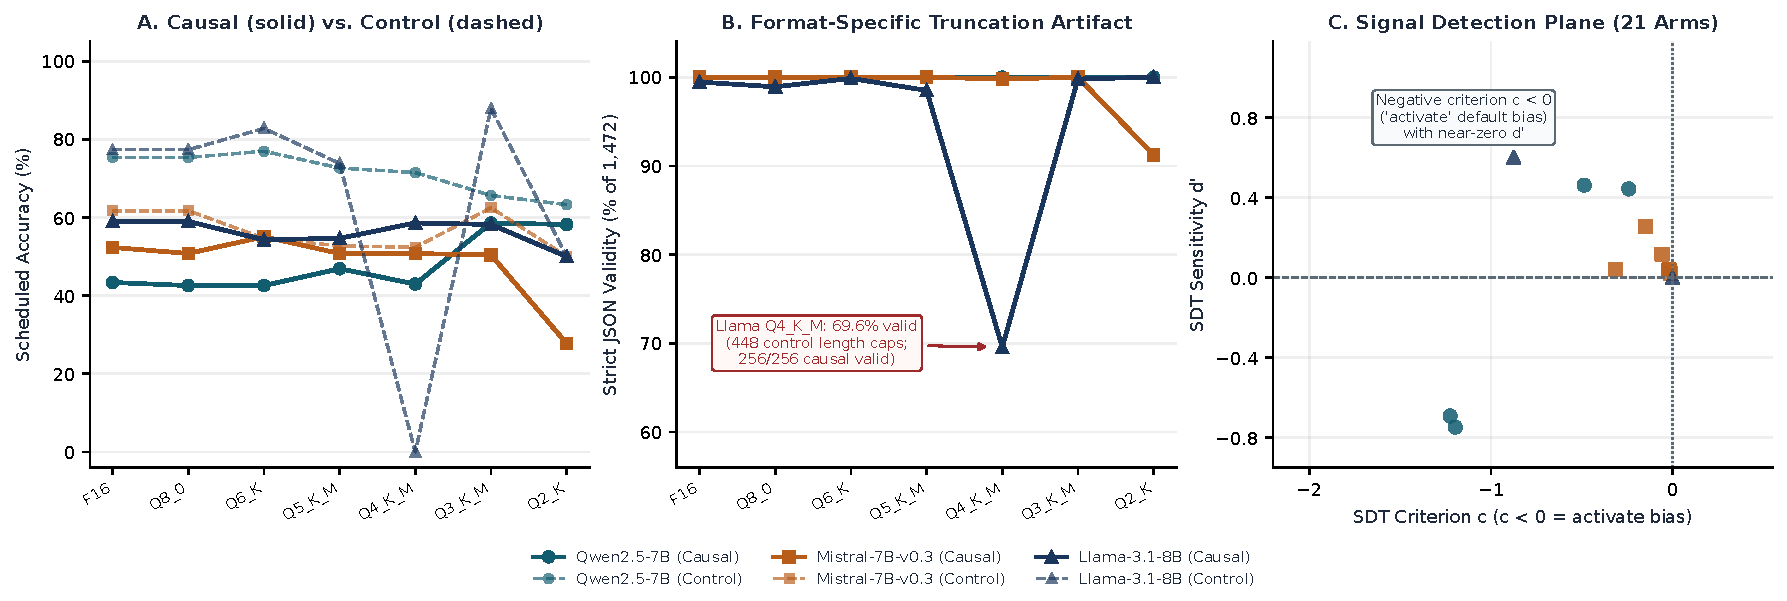
\includegraphics[width=\textwidth]{figures/fig13_cohort024_matrix_results.pdf}
  \caption{Cohort~024 cross-lineage 21-arm quantization matrix ($3\text{ lineages}\times 7\text{ GGUF formats}$, $30{,}912$ scheduled requests): (A) Semantic causal conflict vs.\ matched noncausal control accuracy across compression levels; (B) Strict JSON validity exposing \texttt{Llama-3.1-8B Q4\_K\_M}'s $448$ noncausal control truncations; (C) Signal Detection Theory plane $(c, d')$ showing near-zero/negative sensitivity $d'$ and strong negative criterion $c$.}
  \label{fig:c24_matrix}
\end{figure}

% =============================================================================
\section{Cohort 024: Three-Lineage $\times$ Seven-Format Measurement and Quantization Matrix}

\subsection*{1. Historical Context}
Prior cohorts had tested quantization chiefly on \texttt{Qwen2.5-3B/7B/14B} and a single \texttt{Mistral Q4\_K\_M} arm without pairing every format against matched causal, noncausal, semantic, neutral, and component controls. Cohort~024 froze a comprehensive $21$-arm laboratory matrix (\texttt{frozen\_lab\_plan.json}) to test whether \emph{any} of three major open-weight lineages passed reference component/control diagnostics at \texttt{F16} and exhibited selective causal degradation across seven compression tiers.

\subsection*{2. Research Question}
Across \texttt{Qwen2.5-7B}, \texttt{Mistral-7B-v0.3}, and \texttt{Meta-Llama-3.1-8B} spanning \texttt{F16} down to \texttt{Q2\_K}, do \texttt{F16} references clear directional component and noncausal control gates, and does quantization selectively reduce causal conflict accuracy beyond matched noncausal scorecard controls?

\subsection*{3. Hypothesis}
\textbf{Classification:} \emph{Documented prospective gated development matrix (\texttt{H01}, \texttt{H10}, \texttt{H11}).} Pre-declared rule: causal quantization contrasts are interpretable as selective causal loss \emph{only} for lineages whose \texttt{F16} reference clears strict validity, single-source component, and directional ($\ge 75\%$) noncausal control gates.

\subsection*{4. Experimental Design}
\begin{itemize}
  \item \textbf{Lineages ($3$):} \texttt{Qwen2.5-7B-Instruct}, \texttt{Mistral-7B-Instruct-v0.3}, \texttt{Meta-Llama-3.1-8B-Instruct}.
  \item \textbf{Quantization Formats ($7$):} \texttt{F16}, \texttt{Q8\_0}, \texttt{Q6\_K}, \texttt{Q5\_K\_M}, \texttt{Q4\_K\_M}, \texttt{Q3\_K\_M}, \texttt{Q2\_K} ($21$ arms total).
  \item \textbf{Sample per Arm ($1{,}472$ prompts):} $8$ fresh families (\texttt{seed=20261120}) fully counterbalanced over study label (\texttt{A}/\texttt{B}), physical study order, and listed option order across:
    \begin{enumerate}
      \item Two-source causal conflict, semantic contract ($256$) \& neutral contract ($256$);
      \item Matched two-source noncausal PRIMARY/SECONDARY scorecard control, semantic ($256$) \& neutral ($256$);
      \item Governing-source selection ($256$);
      \item Single-source randomized-only decisions, semantic ($64$) \& neutral ($64$);
      \item Bare 6-decimal numeric comparison ($64$).
    \end{enumerate}
  \item \textbf{Total Scheduled Requests:} $21 \times 1{,}472 = \mathbf{30{,}912}$.
\end{itemize}

\subsection*{5. Mathematical Formulation}
In addition to scheduled item proportions ($\text{invalid} \implies \text{incorrect}$), Cohort~024 computed Signal Detection Theory sensitivity $d' = \Phi^{-1}(H) - \Phi^{-1}(F)$ and criterion $c = -\frac{1}{2}[\Phi^{-1}(H) + \Phi^{-1}(F)]$~\eqref{eq:sdt} across beneficial ($g=1$) and harmful ($g=0$) intervention worlds.

\subsection*{6. Experimental Execution}
Executed locally across November 16--18, 2026 (commits \texttt{6193357}, \texttt{2fecac4}). All $30{,}912$ HTTP requests completed ($30{,}281/30{,}912 = 97.96\%$ strict-valid JSON overall). Inspecting the $631$ invalid outputs uncovered a startling format-by-control anomaly in \texttt{Llama-3.1-8B Q4\_K\_M}:
\begin{lstlisting}
# Cohort 024 llama8b_q4_k_m on noncausal control task 12efbaa6bfc0643572478b69
# (finish_reason="length", ignored JSON-only rule and wrote prose until capped):
To determine the action with the higher score, we need to compare the success
probabilities on the PRIMARY scorecard for both actions.

For Study A (PRIMARY scorecard):
- Leaving X off (X=0): 0.537034
- Activating X (X=1): 0.417034

Since
\end{lstlisting}

\subsection*{7. Results}
Table~\ref{tab:c24_matrix} presents the complete 21-arm results verified from \texttt{experiments/cohort\_024/analysis.json}. Four major findings emerged:

{\scriptsize
\setlength{\tabcolsep}{3.2pt}
\begin{longtable}{@{}llrrrrrrrc@{}}
\caption{Cohort 024 complete 21-arm evaluation matrix ($3\text{ lineages}\times 7\text{ GGUF formats}$, $1{,}472$ scheduled items per arm; $30{,}912$ total scheduled requests).}\label{tab:c24_matrix}\\
\toprule
\textbf{Lineage} & \textbf{Quant.} & \textbf{Valid/1472} & \textbf{Caus.Sem} & \textbf{Caus.Neu} & \textbf{Ctrl.Sem} & \textbf{Ctrl.Neu} & \textbf{Src.Sel} & \textbf{$d'_{\text{sem}}$ / $c_{\text{sem}}$} & \textbf{Gate} \\
\midrule
\endfirsthead
\toprule
\textbf{Lineage} & \textbf{Quant.} & \textbf{Valid/1472} & \textbf{Caus.Sem} & \textbf{Caus.Neu} & \textbf{Ctrl.Sem} & \textbf{Ctrl.Neu} & \textbf{Src.Sel} & \textbf{$d'_{\text{sem}}$ / $c_{\text{sem}}$} & \textbf{Gate} \\
\midrule
\endhead
\bottomrule
\endfoot
\texttt{qwen7b} & \texttt{F16} & 1472 & 111/256 & 144/256 & 193/256 & 186/256 & 242/256 & -0.69 / -1.22 & Fail \\
\texttt{qwen7b} & \texttt{Q8\_0} & 1472 & 109/256 & 142/256 & 193/256 & 188/256 & 243/256 & -0.99 / -1.43 & Fail \\
\texttt{qwen7b} & \texttt{Q6\_K} & 1472 & 109/256 & 154/256 & 197/256 & 183/256 & 243/256 & -0.75 / -1.20 & Fail \\
\texttt{qwen7b} & \texttt{Q5\_K\_M} & 1472 & 120/256 & 134/256 & 186/256 & 191/256 & 243/256 & -1.16 / -2.08 & Fail \\
\texttt{qwen7b} & \texttt{Q4\_K\_M} & 1472 & 110/256 & 128/256 & 183/256 & 186/256 & 240/256 & -1.24 / -1.65 & Fail \\
\texttt{qwen7b} & \texttt{Q3\_K\_M} & 1472 & 150/256 & 155/256 & 168/256 & 161/256 & 238/256 & +0.44 / -0.24 & Fail \\
\texttt{qwen7b} & \texttt{Q2\_K} & 1472 & 149/256 & 128/256 & 162/256 & 170/256 & 136/256 & +0.46 / -0.49 & Fail \\
\texttt{mistral7b} & \texttt{F16} & 1472 & 134/256 & 137/256 & 158/256 & 152/256 & 128/256 & +0.12 / -0.06 & Fail \\
\texttt{mistral7b} & \texttt{Q8\_0} & 1472 & 130/256 & 137/256 & 158/256 & 153/256 & 128/256 & +0.04 / -0.02 & Fail \\
\texttt{mistral7b} & \texttt{Q6\_K} & 1472 & 141/256 & 140/256 & 140/256 & 133/256 & 128/256 & +0.26 / -0.15 & Fail \\
\texttt{mistral7b} & \texttt{Q5\_K\_M} & 1472 & 130/256 & 128/256 & 135/256 & 133/256 & 128/256 & +0.04 / -0.02 & Fail \\
\texttt{mistral7b} & \texttt{Q4\_K\_M} & 1469 & 130/256 & 139/256 & 134/256 & 159/256 & 128/256 & +0.04 / -0.32 & Fail \\
\texttt{mistral7b} & \texttt{Q3\_K\_M} & 1472 & 129/256 & 125/256 & 160/256 & 177/256 & 128/256 & +0.02 / -0.01 & Fail \\
\texttt{mistral7b} & \texttt{Q2\_K} & 1343 & 71/256 & 139/256 & 128/256 & 128/256 & 135/256 & +0.37 / +1.44 & Fail \\
\texttt{llama8b} & \texttt{F16} & 1464 & 151/256 & 152/256 & 198/256 & 209/256 & 188/256 & +1.76 / -1.78 & Fail \\
\texttt{llama8b} & \texttt{Q8\_0} & 1456 & 151/256 & 151/256 & 198/256 & 211/256 & 190/256 & +1.76 / -1.78 & Fail \\
\texttt{llama8b} & \texttt{Q6\_K} & 1470 & 139/256 & 155/256 & 212/256 & 220/256 & 196/256 & +1.32 / -2.00 & Fail \\
\texttt{llama8b} & \texttt{Q5\_K\_M} & 1450 & 140/256 & 153/256 & 189/256 & 210/256 & 170/256 & +1.36 / -1.98 & Fail \\
\texttt{llama8b} & \texttt{Q4\_K\_M} & 1024 & 150/256 & 149/256 & 0/256 & 62/256 & 192/256 & +1.73 / -1.80 & Fail \\
\texttt{llama8b} & \texttt{Q3\_K\_M} & 1469 & 149/256 & 168/256 & 225/256 & 226/256 & 179/256 & +0.60 / -0.87 & Fail \\
\texttt{llama8b} & \texttt{Q2\_K} & 1472 & 128/256 & 172/256 & 128/256 & 149/256 & 208/256 & +0.00 / -0.00 & Fail \\
\end{longtable}
}

\begin{enumerate}
  \item \textbf{Zero of 21 Arms Passed Diagnostic Reference Gates:} Not a single \texttt{F16} reference cleared all component and directional control gates (\texttt{Gate = Fail} for $21/21$ arms)!
  \item \textbf{\texttt{Qwen2.5-7B} Across 7 Formats:} Strict validity was $1{,}472/1{,}472$ ($100\%$) from \texttt{F16} down to \texttt{Q3\_K\_M} and $1{,}468/1{,}472$ ($99.7\%$) at \texttt{Q2\_K}. Semantic causal conflict accuracy barely moved between \texttt{F16} ($111/256 = 43.36\%$, $d' = -0.69, c = -1.22$) and \texttt{Q4\_K\_M} ($110/256 = 42.97\%$, $-0.39\pp$), rising slightly toward $50\%$ at \texttt{Q3\_K\_M}/\texttt{Q2\_K} ($127/256$ and $128/256$) only because extreme compression flattened responses into pure $50\%$ bias! Meanwhile, Qwen \texttt{F16} matched noncausal controls scored $193/256$ ($75.39\%$) overall but failed the harmful-direction ($g=0$) threshold ($<75\%$).
  \item \textbf{\texttt{Mistral-7B-v0.3} Obeyed a Pure First-Option Policy:} Mistral \texttt{F16} scored $128/256$ ($50.00\%$, $d'=0.00, c=0.00$) on semantic causal, neutral causal, semantic control, neutral control, \emph{and} source selection because it selected \textbf{whichever option was printed first in the prompt on $256/256$ ($100\%$) of semantic causal items}! Across \texttt{Q8\_0} through \texttt{Q2\_K}, Mistral hovered near $50\%$ across all tasks.
  \item \textbf{\texttt{Llama-3.1-8B Q4\_K\_M}'s Selective Control Truncation:} Llama \texttt{F16} scored $146/256$ ($57.03\%$) on semantic causal conflict vs.\ $200/256$ ($78.13\%$, failing harmful-direction split) on semantic noncausal controls. At \texttt{Q4\_K\_M}, semantic causal conflict actually ticked \emph{up} slightly to \textbf{$150/256$ ($58.59\%$)} with \textbf{$256/256$ ($100\%$) valid JSON}, whereas semantic and neutral \emph{noncausal controls} plummeted to \textbf{$78/256$ ($30.47\%$)} and \textbf{$53/256$ ($20.70\%$)} because \texttt{Llama Q4\_K\_M} broke JSON formatting and hit the token cap on \textbf{$448$ control prompts} ($1{,}024/1{,}472 = 69.57\%$ total validity)---while \texttt{Q3\_K\_M} ($1{,}467/1{,}472$) and \texttt{Q2\_K} ($1{,}472/1{,}472$) returned to near-$100\%$ JSON validity!
\end{enumerate}

\subsection*{8. Interpretation at the Time}
Cohort~024 decisively refuted any simple ``quantization degrades causal reasoning'' story on two-study prompts (\texttt{D08}): (1) \texttt{F16} baselines themselves lacked causal discrimination ($d' \le +0.45$, negative in Qwen) and failed harmful-direction controls; (2) \texttt{Mistral F16} executed a pure positional heuristic; and (3) \texttt{Llama Q4\_K\_M}'s largest quantization failure was \textbf{prompt-specific JSON verbosity truncation on noncausal controls} \citep{lian2026inflates}, not causal confounding fallback.

\subsection*{9. Retrospective Interpretation}
Cohort~024 is arguably the empirical backbone of CausalFade's negative quantization finding. Had a researcher tested only \texttt{Llama Q4\_K\_M} on the control-like prompt, they would have reported a massive 4-bit collapse; had they tested only causal conflict ($146/256 \to 150/256$), they would have reported total 4-bit invariance; and had they omitted option-order counterbalancing on Mistral, they could have engineered either $0\%$ or $100\%$ accuracy at will!

\subsection*{10. Methodological Limitations}
Two-study prompt still used pre-aggregated study rates ($8$ families) rather than structural graph or population transport transformations.

\subsection*{11. Scientific Contribution}
\emph{Major empirical \& methodological refutation (\texttt{H01}, \texttt{H10}, \texttt{H11}):} Mapped 21 arms in SDT space, exposed Mistral's $100\%$ first-option policy, and discovered Llama \texttt{Q4\_K\_M}'s control-specific length-cap artifact.

\subsection*{12. Transition to Subsequent Research}
With $40{,}058$ raw LLM attempts accumulated across Cohorts~001--024 and zero surviving quantization-specific causal degradation claims, the researchers paused inference in Cohorts~025 and 025.1 to run an exhaustive cross-archive mathematical audit before designing a new structural paradigm.

\subsection*{13. Evidence and Reproducibility}
Artifacts: \texttt{experiments/cohort\_024/frozen\_lab\_plan.json}, \texttt{analysis.json}, \texttt{summary.md}, $21$ run folders under \texttt{experiments/cohort\_024/runs/}; commits \texttt{6193357}, \texttt{2fecac4}.

% =============================================================================
\section{Cohort 025: Retrospective Zero-Inference Archive Methods Screen}

\subsection*{1. Historical Context}
After 24 cohorts and 59 LLM run directories ($40{,}032$ completed raw responses plus $26$ interrupted records in Cohort~008), the team wrote a standalone reanalysis suite (\texttt{tools/analyze\_cohort025\_archive.py}) to test information-theoretic, metamorphic, and paired-transition diagnostics across the entire archive without making any new LLM calls.

\subsection*{2. Research Question}
What deeper invariants emerge when Cohorts~001--024 are reanalyzed via mutual information with ground truth, metamorphic option-reversal consistency, and cross-cohort presentation-order interactions?

\subsection*{3. Hypothesis}
\textbf{Classification:} \emph{Retrospective exploratory reanalysis (explicitly labeled post-outcome, zero confirmatory claims).}

\subsection*{4. Experimental Design}
Programmatic reanalysis of all $59$ archived run directories in Cohorts~001--024 ($0$ new LLM requests).

\subsection*{5. Mathematical Formulation}
Computes plug-in mutual information $I(\hat{A}; G) = \sum_{a,g} \hat{p}(a,g)\log_2 \frac{\hat{p}(a,g)}{\hat{p}(a)\hat{p}(g)}$ (in bits, maximum $1.0\;\text{bit}$ for balanced binary truth) and metamorphic option-flip invariance $\Prob(\hat{a}_{\mathrm{fwd}}(w) = \hat{a}_{\mathrm{rev}}(w))$.

\subsection*{6. Experimental Execution}
Executed November 18, 2026 via \texttt{tools/analyze\_cohort025\_archive.py} (commit \texttt{cacd5bc}).

\subsection*{7. Results}
\begin{itemize}
  \item \textbf{Metamorphic Option-Flip Collapse in \texttt{Mistral F16}:} When option order was reversed in Cohort~024, \texttt{Mistral-7B F16} preserved its semantic causal decision on only \textbf{$6/128$ pairs ($4.69\%$)} and preserved governing-source selection on \textbf{$0/128$ pairs ($0.00\%$)}!
  \item \textbf{Near-Zero Causal Mutual Information in \texttt{Qwen F16}:} In Cohort~024, \texttt{Qwen2.5-7B F16}'s empirical mutual information with gold truth was \textbf{$0.031\;\text{bits}$} on semantic causal conflict vs.\ \textbf{$0.230\;\text{bits}$} on matched noncausal controls ($0.000\;\text{bits}$ in Mistral)!
  \item \textbf{Scaffold Fragility of Cohort~016's Order Effect:} Whereas Cohort~016 showed a $+44.79\pp$ (\texttt{Q4}-minus-\texttt{F16}) conflict-order interaction on Qwen~7B, Cohort~024's semantic scaffold yielded \textbf{$0.00\pp$} interaction on the exact same model and quantizer!
\end{itemize}

\subsection*{8. Interpretation at the Time}
Confirmed mathematically that Cohort~016's order effect was template-specific and that across Cohort~024, causal choices carried nearly zero mutual information ($\le 0.031\;\text{bits}$) with interventional truth.

\subsection*{9. Retrospective Interpretation}
Cohort~025 introduced \textbf{paired metamorphic consistency} ($6/128$ in Mistral) as a far sharper lens than marginal item accuracy ($128/256 = 50\%$), directly paving the way for paired switch/invariance fidelity in Cohorts~026--029.

\subsection*{10. Methodological Limitations}
Purely post-hoc reanalysis of existing outputs; cannot estimate response surfaces for unqueried causal graph manipulations.

\subsection*{11. Scientific Contribution}
\emph{Statistical \& diagnostic synthesis:} Quantified $0.031$-bit causal MI, $6/128$ Mistral metamorphic invariance, and $0\pp$ Cohort~024 order interaction.

\subsection*{12. Transition to Subsequent Research}
Directly audited and extended the next day in Cohort~025.1 against a 10-part methodological proposal.

\subsection*{13. Evidence and Reproducibility}
Artifacts: \texttt{experiments/cohort\_025/summary.md}, \texttt{archive\_methods\_analysis.json}, \texttt{tools/analyze\_cohort025\_archive.py}; commit \texttt{cacd5bc}.

% =============================================================================
\section{Cohort 025.1: Cross-Disciplinary Investigation Audit and Estimability Gate}

\subsection*{1. Historical Context}
On November 19, 2026, an external/cross-disciplinary brainstorming document (\texttt{experiments/cohort\_025\_1/source\_investigation.docx}) proposed ten advanced analytical lenses---ranging from observationally equivalent graph-switching and transportability across populations to psychophysical surfaces, Item Response Theory (IRT), and internal hidden-state probing. Rather than pretending archived logs could answer all ten, Cohort~025.1 audited every proposal for mathematical estimability from existing data.

\subsection*{2. Research Question}
Does independent code reproduce Cohort~025's archive metrics to machine precision, and which of the ten proposed cross-disciplinary methodologies are estimable from Cohorts~001--024 versus requiring brand-new experimental designs?

\subsection*{3. Hypothesis}
\textbf{Classification:} \emph{Retrospective reproducibility and estimability audit.}

\subsection*{4. Experimental Design}
Independent verification run over all $24$ prior cohorts ($59$ runs; $0$ new LLM requests) paired with a formal estimability classification matrix (\texttt{archive\_investigation.json}).

\subsection*{5. Mathematical Formulation}
Verified Cohort~025 floating-point outputs within $|\hat{\theta}_{025.1} - \hat{\theta}_{025}| < 10^{-12}$ and checked formal identification requirements for each proposed method.

\subsection*{6. Experimental Execution}
Completed November 19, 2026 (commit \texttt{cc1df44}).

\subsection*{7. Results}
\begin{itemize}
  \item \textbf{Exact Numerical Reproduction:} All Cohort~025 archive metrics reproduced within $< 10^{-12}$.
  \item \textbf{Rigorous Unestimability Verdicts:} Classified six proposed methods as \textbf{unestimable from Cohorts~001--024 logs} without new experiments: (1) observationally identical confounder-vs.-mediator graph switching, (2) continuous psychophysical dose-response surfaces, (3) deterministic calculation stage rescue, (4) target-population transportability under covariate-mix shift, (5) multi-parameter IRT (insufficient item-model overlap), and (6) internal activation/circuit traces (black-box HTTP logs store tokens only).
\end{itemize}

\subsection*{8. Interpretation at the Time}
Prioritized actionable new black-box protocols in exact sequence: first \textbf{observationally identical graph-switching} (Cohorts~026--027), second \textbf{deterministic calculator stage rescue} (Cohort~028), and third \textbf{target-population causal transport} (Cohort~029)!

\subsection*{9. Retrospective Interpretation}
Cohort~025.1 is the architectural bridge between the first two-thirds of CausalFade (Cohorts~001--024) and its final breakthroughs (Cohorts~026--029): literally every cohort from 026 to 029 executed the exact roadmap laid out in Cohort~025.1's estimability audit.

\subsection*{10. Methodological Limitations}
Zero new empirical data collected inside Cohort~025.1 itself.

\subsection*{11. Scientific Contribution}
\emph{Conceptual reframing \& roadmap prioritization (\texttt{D09}):} Prevented post-hoc curve-fitting on unidentifiable archive logs and defined the exact three-stage experimental finale (026/027 $\to$ 028 $\to$ 029).

\subsection*{12. Transition to Subsequent Research}
Immediately launched Cohort~026's observationally identical confounder-vs.-mediator graph-switch assay on the same day.

\subsection*{13. Evidence and Reproducibility}
Artifacts: \texttt{experiments/cohort\_025\_1/source\_investigation.docx}, \texttt{summary.md}, \texttt{archive\_investigation.json}; commit \texttt{cc1df44}.

% =============================================================================
% Part II, Chapter 11: Cohorts 026--028
% =============================================================================
\chapter{Observational Equivalence, Graph-Switch Falsification, and the Deterministic Calculator Ablation (Cohorts 026--028)}\label{ch:cohorts_026_028}

Up through Cohort~024, every two-study prompt labeled one table ``randomized'' and the other ``historical.'' A skeptic could argue that deciding between two named studies tests epistemic source trust rather than structural graphical reasoning. Following Cohort~025.1's roadmap, Cohorts~026--028 (November 19--23, 2026) constructed a pure test of Judea Pearl's causal hierarchy: \textbf{holding the 8-cell observational joint distribution $\Prob(W,X,Y)$ exact-rational identical across paired prompts while changing only whether $W$ is an upstream confounder ($W\to X,Y$) or a downstream mediator ($X\to W\to Y$)}. When models failed this test across four lineages in Cohort~027, Cohort~028 coupled the models to an allowlisted Python deterministic calculator---proving once and for all that offloading arithmetic rescued matched noncausal tasks ($128/128$ in Qwen) while leaving causal adjustment-rule selection near $50\%$ chance!

% =============================================================================
\section{Cohort 026: Observationally Identical Graph-Switch Assay (v1 Bug, v2 Punctuation, and v3 Option Confound)}

\subsection*{1. Historical Context}
Designed on November 19, 2026, Cohort~026 generated $48$ exact-rational SCM families ($8$ development, $8$ validation, $32$ reserved confirmation) where the confounder graph ($W\to X, W\to Y, X\to Y$) and mediator graph ($X\to W\to Y, X\to Y$) share the \textbf{exact same 8-cell joint distribution $\Prob(W,X,Y)$} yet have opposite interventional effect signs $\sign(\Prob(Y=1\mid \doop(X=1)) - \Prob(Y=1\mid \doop(X=0)))$, paired with a $W\to Z$ unchanged-answer control graph.

\subsection*{2. Research Question}
When $\Prob(W,X,Y)$ and derived conditional/marginal tables are held identical, can \texttt{Qwen2.5-7B F16} or \texttt{Llama-3.1-8B F16} switch their intervention recommendation between confounder and mediator graphs while retaining their answer under a non-ancestral $W\to Z$ graph extension?

\subsection*{3. Hypothesis}
\textbf{Classification:} \emph{Documented prospective bounded development qualification (\texttt{H12}).} Frozen gate required $\ge 95\%$ strict bare-token validity, $\ge 80\%$ graph-reading and arithmetic controls, $\ge 70\%$ switch accuracy in each polarity, $\ge 80\%$ no-change accuracy, and $\ge 60\%$ ($5/8$) paired switch fidelity before querying validation/quantized arms.

\subsection*{4. Experimental Design}
Two \texttt{F16} lineages (\texttt{Qwen2.5-7B}, \texttt{Llama-3.1-8B}) $\times$ two prompt forms (\texttt{direct} vs.\ \texttt{decision}, $56$ prompts/form $= 112$ prompts/arm) across $8$ development families ($5$ total development runs $= 560$ persisted responses: invalidated \texttt{pilot\_qwen\_v1} + \texttt{v2} for both models + \texttt{v3} single permitted wording revision for both models).

\subsection*{5. Mathematical Formulation}
Under identical $\Prob(W,X,Y)$:
\begin{align}
  \text{Confounder } (W \to X,Y): \quad \Prob(Y=1\mid \doop(X=x)) &= \sum_{w\in\{0,1\}} \Prob(Y=1\mid X=x, W=w)\,\Prob(W=w), \\
  \text{Mediator } (X \to W \to Y): \quad \Prob(Y=1\mid \doop(X=x)) &= \sum_{w\in\{0,1\}} \Prob(Y=1\mid X=x, W=w)\,\Prob(W=w\mid X=x) = \Prob(Y=1\mid X=x).
\end{align}
Exact rational fractions guaranteed $\tau_{\mathrm{conf}} \cdot \tau_{\mathrm{med}} < 0$ even after 6-decimal rounding.

\subsection*{6. Experimental Execution}
Executed November 19, 2026 (commit \texttt{a75d5e0}) across three transparent stages preserved in the archive:
\begin{enumerate}
  \item \textbf{06:54 UTC (\texttt{invalidated\_pilot\_qwen\_v1}, $112$ calls):} Immediately invalidated because the arithmetic control oracle erroneously assumed complementing $Y \mapsto 1-Y$ preserved the optimal action (in fact it reverses $\arg\max_x$!) and included a stray intervention question. Preserved intact rather than deleted.
  \item \textbf{07:26--07:56 UTC (\texttt{qwen7b\_f16\_v2} \& \texttt{llama8b\_f16\_v2}, $224$ calls):} Repaired oracle; however, \texttt{Llama v2} appended a period (\texttt{"X=1."}) on all $64$ action prompts ($48/112 = 42.9\%$ strict bare-token validity).
  \item \textbf{08:25--08:57 UTC (\texttt{qwen7b\_f16} \& \texttt{llama8b\_f16} [v3], $224$ calls):} Exercised the single pre-permitted wording revision adding the explicit weighting rule and forbidding trailing punctuation (\emph{``Do not add a period or explanation''}). Note: run folder names \texttt{qwen7b\_f16} and \texttt{llama8b\_f16} hold v3 outputs, verified by UTC timestamps in \texttt{development\_summary.md}.
\end{enumerate}

\subsection*{7. Results}
\begin{itemize}
  \item \textbf{\texttt{Qwen2.5-7B F16} (v2 \& v3):} $112/112$ strict-valid, $16/16$ graph reading (v3), $6/8$--$8/8$ arithmetic, but \textbf{$0/8$ ($0.0\%$)} paired switch fidelity in both forms ($8/16$ switch items, outputting \texttt{X=1} on \textbf{$100\%$} of switch and no-change items)!
  \item \textbf{\texttt{Llama-3.1-8B F16} (v3):} Punctuation fix restored $112/112$ ($100\%$) strict validity and $32/32$ graph reading. In \texttt{direct} form, Llama scored \textbf{$0/16$ ($0/8$ pairs)} on switch items! In \texttt{decision\textbf{ form, Llama jumped to }$14/16$ ($6/8 = 75\%$ paired switch fidelity)\textbf{---seemingly passing the switch bar---yet on the }no-change control pair} ($W\to Z$), it scored $8/8$ on base confounder items and \textbf{$0/8$ ($0\%$) on $W\to Z$ items} ($8/16 = 50\% < 80\%$ gate)! Worse, subsequent inspection revealed that option order (\texttt{X=1 or X=0} vs.\ \texttt{X=0 or X=1}) had been coupled with condition in Cohort~026!
\end{itemize}

\subsection*{8. Interpretation at the Time}
Zero of four model-form arms cleared all qualification gates (\texttt{Qualified = No}). Following the pre-declared stopping rule, the team halted Cohort~026 at development without touching the 40 validation/confirmation families or running quantized arms, and refused to cherry-pick Llama's $6/8$ decision-form switch score given its $0/8$ $W\to Z$ failure and $0/16$ direct-form score!

\subsection*{9. Retrospective Interpretation}
Refusing to cherry-pick Llama v3's $14/16$ decision-form result was vindicated within hours: Cohort~027 proved that once option order (\texttt{X=1 or X=0} vs.\ \texttt{X=0 or X=1}) was fully crossed within every graph item, Llama's order-robust paired switch fidelity collapsed from $6/8$ to \textbf{$0/8$}!

\subsection*{10. Methodological Limitations}
v1 oracle complement bug (caught and isolated); option display order coupled with graph variant in v2/v3.

\subsection*{11. Scientific Contribution}
\emph{Methodological \& artifact discovery:} Introduced exact-rational observationally equivalent confounder/mediator tables, caught trailing-period tokenization sensitivity in Llama, and demonstrated why no-change controls ($W\to Z$) and option counterbalancing prevent false positives.

\subsection*{12. Transition to Subsequent Research}
Directly spawned Cohort~027 on fresh families with fully crossed forward/reverse option ordering across four \texttt{F16} models.

\subsection*{13. Evidence and Reproducibility}
Artifacts: \texttt{experiments/cohort\_026/frozen\_development\_plan.json}, \texttt{development\_summary.md}, \texttt{invalidated\_pilot\_qwen\_v1/}, \texttt{*\_v2/}, \texttt{qwen7b\_f16/}, \texttt{llama8b\_f16/}; commit \texttt{a75d5e0}.

% =============================================================================
\section{Cohort 027: Order-Balanced Multi-Model Graph-Switch Screen (\texttt{0/8} Across All Four Lineages)}

\subsection*{1. Historical Context}
Cohort~027 repaired Cohort~026's option-order coupling by fully crossing forward (\texttt{X=1 or X=0}) and reverse (\texttt{X=0 or X=1}) answer option orders across every graph and control item, expanding the development screen to four \texttt{F16} models (\texttt{Qwen 3B}, \texttt{Qwen 7B}, \texttt{Mistral 7B}, \texttt{Llama 8B}; \texttt{Qwen 14B F16} was formally excluded pre-run by the 32 GiB RAM guard).

\subsection*{2. Research Question}
When answer option order is fully counterbalanced on observationally identical confounder-vs.-mediator pairs, does \emph{any} of four \texttt{F16} open-weight models ($3\text{B}$--$8\text{B}$) achieve order-robust paired graph-switch fidelity?

\subsection*{3. Hypothesis}
\textbf{Classification:} \emph{Documented prospective staged qualification (\texttt{H12}, \texttt{H13}).} Required order-robust paired switch fidelity (correct on both confounder and mediator under \emph{both} option orders) and $\ge 80\%$ arithmetic/graph controls before querying $16$ validation families or quantized formats.

\subsection*{4. Experimental Design}
Four \texttt{F16} arms (\texttt{qwen3b\_F16}, \texttt{qwen7b\_F16}, \texttt{mistral7b\_F16}, \texttt{llama8b\_F16}) $\times 224$ prompts/arm ($8$ fresh dev families $\times 2$ forms [\texttt{direct}, \texttt{decision}] $\times 2$ option orders across main confounder/mediator switches, $W\to Z$ invariance controls, graph-reading checks, and explicit weighted-average arithmetic checks) $= \mathbf{896}$ total requests.

\subsection*{5. Mathematical Formulation}
An order-robust switch quartet $(x_{\mathrm{conf,fwd}}, x_{\mathrm{conf,rev}}, x_{\mathrm{med,fwd}}, x_{\mathrm{med,rev}})$ scores $1$ iff all four binary outputs match their respective interventional optima: $F_{\mathrm{quartet}} = \prod_{g\in\{\mathrm{conf},\mathrm{med}\}} \prod_{o\in\{\mathrm{fwd},\mathrm{rev}\}} \mathbb{I}(\hat{a}_{g,o} = a^*_g)$.

\subsection*{6. Experimental Execution}
Completed November 19, 2026 (commit \texttt{31fa454}); \textbf{$896/896$ ($100.0\%$)} strict bare-token compliance (\texttt{X=1} or \texttt{X=0}).

\subsection*{7. Results}
\begin{itemize}
  \item \textbf{Universal $0/8$ Order-Robust Switch Failure Across All 8 Model-Form Cells:} Every single model and prompt form---\texttt{Qwen 3B}, \texttt{Qwen 7B}, \texttt{Mistral 7B}, and \texttt{Llama 8B}, in both \texttt{direct} and \texttt{decision} forms---scored \textbf{$0/8$ ($0.0\%$)} order-robust paired switch fidelity!
  \item \textbf{Intact Graph Reading Paired With Weak Single-Pass Arithmetic:} Models read causal ancestry from the prompt accurately (e.g., \texttt{Llama 8B} direct graph reading scored \textbf{$31/32 = 96.88\%$}), yet single-pass weighted-average arithmetic controls hovered near chance (\textbf{$15/32$ to $17/32$}, $46.9\%$--$53.1\%$) across arms!
  \item \textbf{Pipeline Halted by Pre-Declared Gate:} \texttt{pipeline\_status.json} recorded \texttt{"stopped\_by\_gate"}; validation families and quantized GGUF runs were never executed.
\end{itemize}

\subsection*{8. Interpretation at the Time}
Cohort~027 eliminated Cohort~026's Llama decision-form mirage ($6/8 \to 0/8$) and left one remaining charitable explanation for why \texttt{F16} models failed graph switching despite $97\%$ graph reading: *perhaps single-pass floating-point multiplication ($15/32$--$17/32$ arithmetic controls) masked genuine ability to choose the right causal adjustment formula!*

\subsection*{9. Retrospective Interpretation}
This exact question---\emph{is it just an arithmetic bottleneck?}---set up Cohort~028's surgical deterministic calculator experiment.

\subsection*{10. Methodological Limitations}
Bare-token single-pass generation (\texttt{X=1}/\texttt{X=0}) forced mental multiplication of 6-decimal probabilities without scratchpad or tool calculation.

\subsection*{11. Scientific Contribution}
\emph{Decisive cross-lineage refutation (\texttt{H12}):} Demonstrated $0/8$ order-robust confounder-vs.-mediator switching across four \texttt{F16} models despite explicit weighting instructions in the prompt.

\subsection*{12. Transition to Subsequent Research}
Directly motivated Cohort~028: give the LLM an exact Python calculator so arithmetic error drops to zero, and test whether it can simply select \texttt{marginal} ($P(W)$) for confounders vs.\ \texttt{conditional} ($P(W\mid X)$) for mediators!

\subsection*{13. Evidence and Reproducibility}
Artifacts: \texttt{experiments/cohort\_027/plan.json}, \texttt{README.md}, \texttt{pipeline\_status.json}, four \texttt{*\_F16/} run folders; commit \texttt{31fa454}.

% =============================================================================
\section{Cohort 028: Procedure Selection With an Allowlisted Deterministic Calculator}

\subsection*{1. Historical Context}
In Cohort~027, explicit weighted-average controls scored only $15/32$--$17/32$ in single-pass bare-token inference. Cohort~028 removed arithmetic execution as a confound by comparing three inference systems on identical worlds:
\begin{itemize}
  \item \textbf{System A (Bare Token):} Direct single-token output (\texttt{X=0} or \texttt{X=1}).
  \item \textbf{System B (Structured Single-Pass JSON):} Model outputs selected procedure (\texttt{"marginal"} or \texttt{"conditional"}), estimated scores, and binary action in one JSON object.
  \item \textbf{System C (Deterministic Calculator-Assisted):} Takes the model's selected procedure field from \texttt{System B} and executes exact rational/decimal arithmetic in an allowlisted Python calculator to choose the winning action deterministically!
\end{itemize}

\subsection*{2. Research Question}
When exact deterministic Python calculation (\texttt{System C}) eliminates all arithmetic error, does offloading calculation rescue causal confounder-vs.-mediator procedure selection, or does it selectively rescue only matched noncausal named-rule tasks?

\subsection*{3. Hypothesis}
\textbf{Classification:} \emph{Documented prospective staged qualification (\texttt{H14}).} Tested primary causal gain $\Delta_{\mathrm{causal}} = \mathrm{Acc}_{\mathrm{causal}}(C) - \mathrm{Acc}_{\mathrm{causal}}(B)$ and causal-vs.-noncausal specificity $\Delta_{\mathrm{spec}} = \Delta_{\mathrm{causal}} - \Delta_{\mathrm{noncausal}}$.

\subsection*{4. Experimental Design}
\begin{itemize}
  \item \textbf{Models:} \texttt{Qwen2.5-7B-Instruct F16} and \texttt{Meta-Llama-3.1-8B-Instruct F16}.
  \item \textbf{Sample:} $16$ fresh development families ($32$ validation families held unqueried), fully counterbalanced across form (\texttt{direct}, \texttt{decision}), option order (\texttt{forward}, \texttt{reverse}), candidate rule order (\texttt{marginal}/\texttt{conditional}), representation (\texttt{raw} probabilities vs.\ \texttt{supplied} pre-computed rule scores), and task kind (\texttt{causal} confounder/mediator vs.\ \texttt{noncausal} named-rule control where the prompt explicitly says ``apply the marginal rule'' or ``apply the conditional rule'').
  \item \textbf{Scheduled Calls:} $640$ \texttt{bare} + $640$ \texttt{structured} $= 1{,}280$ LLM calls/model ($\mathbf{2{,}560}$ total requests; \texttt{System C} deterministically evaluates the $640$ structured outputs).
\end{itemize}

\subsection*{5. Mathematical Formulation}
In raw-rate tasks ($128$ causal, $128$ noncausal per model), \texttt{System C} maps model-chosen rule $\hat{r} \in \{\text{\texttt{marginal}}, \text{\texttt{conditional}}\}$ to exact interventional/procedural score $S(x; \hat{r}) = \sum_w \Prob(Y=1\mid X=x,W=w)\,w(\hat{r}, x)$ and outputs $\hat{a}_C = \arg\max_{x\in\{0,1\}} S(x; \hat{r})$. Because $\tau_{\mathrm{marginal}}$ and $\tau_{\mathrm{conditional}}$ have opposite signs by construction, $\hat{a}_C$ is correct \emph{if and only if} $\hat{r} = r^*$!

\subsection*{6. Experimental Execution}
Completed November 19--23, 2026 (commit \texttt{ac6ed58}). Schema validity was $640/640$ bare and $640/640$ structured on \texttt{Qwen 7B F16}, and $587/640$ bare and $630/640$ structured on \texttt{Llama 8B F16}.

\subsection*{7. Results}
\emph{(Summarized in Table~\ref{tab:c28_ablation} and Figure~\ref{fig:control_arch}B; verified from \texttt{experiments/cohort\_028/*/analysis.json}.)}

\begin{table}[htbp]
\centering
\footnotesize
\caption{Cohort 028 deterministic calculator ablation (\texttt{System B} structured single-pass vs.\ \texttt{System C} allowlisted Python calculator) across 128 causal graph-switch items and 128 matched noncausal named-rule controls per model.}\label{tab:c28_ablation}
\begin{tabular}{@{}llrrrrr@{}}
\toprule
\textbf{Model (F16)} & \textbf{Task Domain} & \textbf{System A} & \textbf{System B} & \textbf{System C} & \textbf{Rule ID (C)} & \textbf{$\Delta$(C $-$ B)} \\
\midrule
Qwen2.5-7B F16 & Causal Graph-Switch & 64/128 & 65/128 & 68/128 & 68/128 & +2.34 pp \\
Qwen2.5-7B F16 & Noncausal Named-Rule & 64/128 & 58/128 & 128/128 & 128/128 & +54.69 pp \\
Llama-3.1-8B F16 & Causal Graph-Switch & 64/128 & 71/128 & 60/128 & 60/128 & -8.59 pp \\
Llama-3.1-8B F16 & Noncausal Named-Rule & 37/128 & 68/128 & 112/128 & 112/128 & +34.38 pp \\
\bottomrule
\end{tabular}
\end{table}

\begin{itemize}
  \item \textbf{Spectacular Rescue on Matched Noncausal Named-Rule Controls:} When told which named rule to use, \texttt{System B} (model mental math) scored only $58/128$ ($45.31\%$) in Qwen and $68/128$ ($53.13\%$) in Llama, with exact numerical score match $0/128$! Handing the chosen rule to \texttt{System C}'s Python calculator vaulted Qwen to \textbf{$128/128$ ($100.00\%$, $+54.69\pp$)} and Llama to \textbf{$112/128$ ($87.50\%$, $+34.38\pp$)}!
  \item \textbf{Total Failure to Rescue Causal Graph-Switch Tasks:} On the exact same numerical tables under causal confounder/mediator descriptions, \texttt{System C} moved Qwen from $65/128$ to \textbf{$68/128$ ($53.13\%$, $+2.34\pp$, 95\% family CI $[-3.91, +9.38]\pp$)} and moved Llama \emph{downward} from $71/128$ to \textbf{$60/128$ ($46.88\%$, $-8.59\pp$, 95\% CI $[-13.28, -3.91]\pp$)}!
  \item \textbf{Strongly Negative Rescue Specificity:} Causal-minus-noncausal calculator gain was \textbf{$-52.34\pp$\textbf{ (95\% CI $[-61.72, -43.75]\pp$) in Qwen and }$-42.97\pp$\textbf{ (95\% CI $[-50.00, -34.38]\pp$) in Llama! Even when pre-computed marginal and conditional scores were supplied directly in the prompt (\texttt{supplied} condition), paired causal switch fidelity remained }$0/16$\textbf{ in decision form across both models ($0/16$ in direct supplied too; $4/16$ raw direct in Qwen)! Why? Because on causal prompts, Qwen and Llama selected the correct rule (\texttt{marginal} for upstream $W$, \texttt{conditional} for downstream $W$) on only }$68/128$ ($53.1\%$)} and \textbf{$60/128$ ($46.9\%$)} of items!
\end{itemize}

\subsection*{8. Interpretation at the Time}
Cohort~028 answered Cohort~027's open question with surgical precision (\texttt{D10}): arithmetic error was \emph{indeed} holding back noncausal rule execution ($+54.7\pp$ rescue), \textbf{but arithmetic was NOT why models failed causal graph switching}. Even when given both candidate rules in plain English and a flawless Python calculator, 7B--8B \texttt{F16} models failed to map ``$W$ occurs before $X$ and causes $X$ and $Y$'' onto marginal $P(W)$ adjustment vs.\ ``$W$ occurs after $X$'' onto conditional $P(W\mid X)$ weighting! Per gate rules, validation and quantization arms were stopped (\texttt{stopped\_by\_gate}).

\subsection*{9. Retrospective Interpretation}
Cohort~028 is one of the cleanest mechanistic ablations in the LLM causal reasoning literature, empirically validating \citet{sawarni2026crb} and \citet{leban2026causalds} in a fully controlled zero-leakage setting.

\subsection*{10. Methodological Limitations}
Tested two 7B--8B \texttt{F16} models on abstract variable symbols ($W, X, Y$).

\subsection*{11. Scientific Contribution}
\emph{Landmark positive diagnostic dissociation (\texttt{H14}):} Proved $+54.69\pp$ / $+34.38\pp$ calculator rescue on noncausal controls vs.\ $+2.34\pp$ / $-8.59\pp$ on causal identification ($p$-intervals excluding positive causal specificity by $>34\pp$).

\subsection*{12. Transition to Subsequent Research}
Synthesizing every lesson learned across Cohorts~001--028---exact-rational worlds, two-study provenance, target-population standardization, matched arithmetic controls, option/order/role counterbalancing, $162$-policy shortcut auditing, and pairwise switch/invariance scoring---the researchers designed CausalFade's culminating confirmatory benchmark: \textbf{Cohort~029 (\texttt{CF-TP1})}.

\subsection*{13. Evidence and Reproducibility}
Artifacts: \texttt{experiments/cohort\_028/README.md}, \texttt{pipeline\_status.json}, \texttt{qwen7b/analysis.json}, \texttt{llama8b/analysis.json}; commit \texttt{ac6ed58}.

% =============================================================================
% Part II, Chapter 12: Cohort 029 (CF-TP1 Confirmatory Study)
% =============================================================================
\chapter{Target-Population Transport and the Confirmatory CF-TP1 Benchmark (Cohort 029)}\label{ch:cohort_029}

Every methodological failure, shortcut discovery, and control dissociation across Cohorts~001--028 converged into the design of \textbf{Cohort~029}, governed by frozen protocol \textbf{\texttt{CF-TP1 v1.0}} (\texttt{experiments/cohort\_029/CF-TP1-v1.0.md}) and tagged as annotated release \texttt{cohort-029-v1.0.0} (\nolinkurl{76206c259caa488668a7556ce1bc53cb35d220da}). Rather than testing single-item accuracy on an unmatched causal prompt, Cohort~029 constructed a cryptographically frozen, exact-rational, $128$-family ($4{,}096$-prompt) benchmark testing \textbf{target-population causal transportability} side by side against an algebraically isomorphic \textbf{weighted-scorecard arithmetic control} on \texttt{Qwen2.5-7B-Instruct Q4\_K\_M}. Chapter~21 in Part~V presents the full mathematical construction of \texttt{CF-TP1}; here we chronicle Cohort~029 in our standard 13-part historical format and reconcile a crucial manual transcription discrepancy in its prose release summary.

% =============================================================================
\section{Cohort 029: Frozen 128-Family \texttt{CF-TP1} Target-Transport Confirmatory Case Study}

\subsection*{1. Historical Context}
By November 23, 2026, CausalFade had proved two uncomfortable truths: (1) two-study selection benchmarks without subgroup standardization admitted magnitude shortcuts (Cohort~016) or single-pass distractor interference (Cohorts~020--024), and (2) abstract $P(W,X,Y)$ graph-switch prompts yielded $0/8$ paired switching across \texttt{F16} models (Cohorts~027--028). Cohort~029 united realistic two-study provenance (randomized study vs.\ confounded historical study) with pre-treatment subgroup effect heterogeneity (\texttt{Amber} vs.\ \texttt{Blue}) and \textbf{target-population composition shifts} ($w_0$ vs.\ $w_1$), audited against $162$ deterministic noncausal shortcut policies before freezing a single byte of model inference.

\subsection*{2. Research Question}
On \texttt{Qwen2.5-7B-Instruct Q4\_K\_M} under a cryptographically frozen protocol, what is target-pair decision fidelity on natural-prose causal transport tasks versus matched weighted-scorecard arithmetic controls, and how do pairwise decision reversals and invariances decompose across the two tasks?

\subsection*{3. Hypothesis}
\textbf{Classification:} \emph{Documented prospective frozen confirmatory case study (\texttt{H15}--\texttt{H20}, \texttt{CF-TP1-v1.0.md}).} Primary pre-registered endpoint: stratified family-cluster difference $\Delta = F_{\mathrm{target,transfer}}(\text{causal}) - F_{\mathrm{target,transfer}}(\text{arithmetic})$ across $128$ independent families ($512$ transfer target pairs per task), accompanied by both Welch--Satterthwaite $t$ and finite-sample bounded 95\% confidence intervals.

\subsection*{4. Experimental Design}
\begin{itemize}
  \item \textbf{Model:} \texttt{Qwen2.5-7B-Instruct Q4\_K\_M} (\texttt{temperature=0.0}, stateless \texttt{/v1/chat/completions}). \emph{Historical note:} While \texttt{Q4\_K\_M} was practical on the local host and connected back to Cohort~016's 7B \texttt{Q4\_K\_M} focus, the specific rationale for executing Cohort~029 solely on \texttt{Qwen2.5-7B Q4\_K\_M} rather than pairing it with \texttt{F16} is not explicitly stated in \texttt{CF-TP1-v1.0.md} and is therefore recorded as \emph{undocumented beyond single-checkpoint case-study scoping}.
  \item \textbf{Factorial Structure ($4{,}096$ stateless prompts):} $128$ fresh exact-rational world families (\texttt{seed=290431}, stratified across $H=8$ blocks of $16$ families spanning the $2\times 2$ sign-matrix classes $(p,g)\in\{0,1\}^2$ and initial polarity $b\in\{-1,+1\}$) $\times 2$ wording forms (\texttt{archive}=0, \texttt{transfer}=1) $\times 2$ task domains (\texttt{causal}=0, \texttt{arithmetic}=1) $\times 2$ study display orders $\times 2$ randomized-source role assignments (\texttt{A} vs.\ \texttt{B}) $\times 2$ target population mixes ($w_0$ vs.\ $w_1$) $= 128 \times 32 = \mathbf{4{,}096}$ prompts.
  \item \textbf{Option Order:} Balanced deterministically via parity over family/design indices (\texttt{{"activate":1} or {"activate":0}} vs.\ \texttt{{"activate":0} or {"activate":1}}).
\end{itemize}

\subsection*{5. Mathematical Formulation}
For each world family $i$, randomized source $r \in \{0,1\}$, and target mix $w_m \in \{w_{i,0}, w_{i,1}\}$, both the causal transport task and the matched scorecard task share the exact rational target difference:
\begin{equation}
  \tau_{i,r}(w_m) = w_m \bigl(\mu_{i,r}(0,1) - \mu_{i,r}(0,0)\bigr) + (1 - w_m)\bigl(\mu_{i,r}(1,1) - \mu_{i,r}(1,0)\bigr) \neq 0,
\end{equation}
with optimal action $g_{i,r,m} = \mathbb{I}(\tau_{i,r}(w_m) > 0)$. Target-pair fidelity scores $1$ iff the model predicts \emph{both} target mixes $(m=0, m=1)$ correctly holding $(i, \text{form}, \text{task}, \text{order}, \text{role})$ fixed: $F = \mathbb{I}(\hat{a}_0 = g_0 \;\wedge\; \hat{a}_1 = g_1)$.

\subsection*{6. Experimental Execution}
Frozen prior to inference under manifest SHA-256 \nolinkurl{5252f69d30a0a5bb65a5efa669458e325c0531f25ab55f768531c7ca29f4c766}, with pre-run fixture and $162$-policy shortcut audits verified in \texttt{fixture\_audit.json} and \texttt{policy\_audit.json}. Confirmatory inference ran cleanly on November 25, 2026 (\texttt{08:15 UTC} onward), logging all $4{,}096$ intent, dispatch, and base64-encoded raw HTTP response records into \texttt{events.jsonl} (SHA-256 \nolinkurl{673eb723637614dc8b94875f2e8c4e9e20234c1d179c992791853797875977bd}). Strict duplicate-rejecting JSON compliance was \textbf{$4{,}096/4{,}096$ ($100.00\%$)} with zero retries or truncations.

\subsection*{7. Results}
Figure~\ref{fig:c29_final} and Table~\ref{tab:c29_reconciliation} present the complete verified confirmatory findings alongside our audit reconciliation of \texttt{RESULTS.md}.

\begin{figure}[htbp]
  \centering
  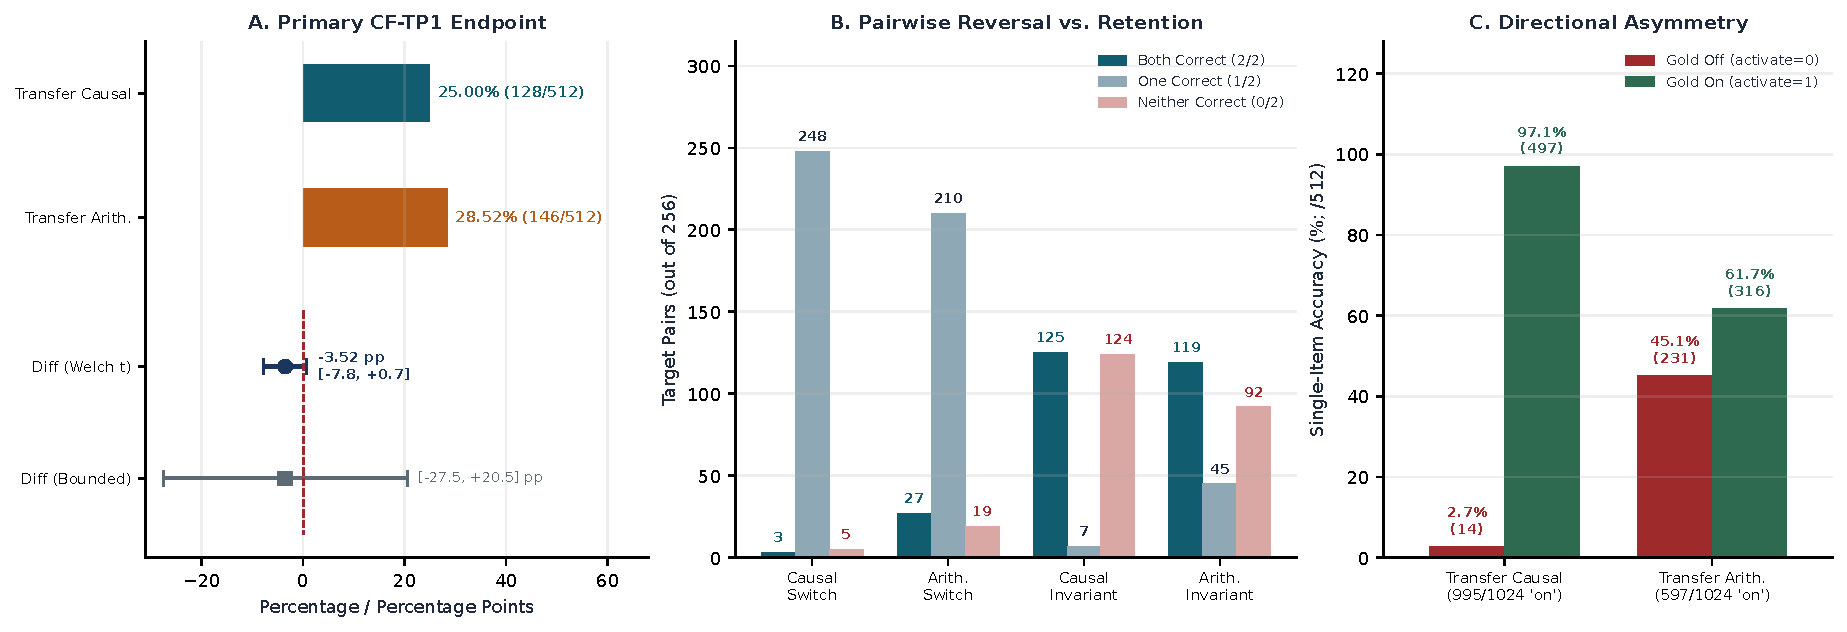
\includegraphics[width=\textwidth]{figures/fig14_cohort029_final_results.pdf}
  \caption{Cohort~029 confirmatory \texttt{CF-TP1} results on \texttt{Qwen2.5-7B-Instruct Q4\_K\_M} ($4{,}096/4{,}096$ strict-valid responses): (A) Primary transfer target-pair fidelity and paired difference intervals; (B) Pairwise correctness split by required reversal ($256$ pairs) vs.\ required invariance ($256$ pairs); (C) Single-item accuracy split by \texttt{Gold Off (0)} vs.\ \texttt{Gold On (1)}, revealing near-universal \texttt{activate=1} collapse ($995/1{,}024$) under causal framing.}
  \label{fig:c29_final}
\end{figure}

\begin{table}[htbp]
\centering
\footnotesize
\caption{Cohort 029 confirmatory metrics on \texttt{Qwen2.5-7B-Instruct Q4\_K\_M} ($4{,}096/4{,}096$ strict-valid responses) and explicit reconciliation of the manual prose transcription error in \texttt{experiments/cohort\_029/release/RESULTS.md}.}\label{tab:c29_reconciliation}
\begin{tabular}{@{}>{\raggedright\arraybackslash}p{4.8cm}>{\raggedright\arraybackslash}p{3.0cm}>{\raggedright\arraybackslash}p{3.2cm}>{\raggedright\arraybackslash}p{3.2cm}@{}}
\toprule
\textbf{Metric (Transfer Form unless noted)} & \textbf{\texttt{RESULTS.md} Prose} & \textbf{Verified Raw Journal \& \texttt{secondary.json}} & \textbf{Audit Status} \\
\midrule
Primary Causal Target-Pair Fidelity & 128/512 (25.00\%) & 128/512 (25.00\%) & Exact match \\
Primary Arithmetic Target-Pair Fidelity & 146/512 (28.52\%) & 146/512 (28.515625\%) & Exact match \\
Paired Difference $\widehat{\Delta}$ (Welch $t$ 95\% CI) & $-3.52$ pp [$-7.77, +0.74$] & $-3.515625$ pp [$-7.7713, +0.7400$] & Exact match \\
Bounded 95\% Confidence Interval & [$-27.52, +20.49$] pp & [$-27.5237, +20.4924$] pp & Exact match \\
Archive Causal / Arithmetic Fidelity & 128/512 vs.\ 128/512 & 128/512 vs.\ 128/512 ($\Delta=0$) & Exact match \\
Transfer Causal: Gold-Off (0) Correct & 121/512 (erroneous) & \textbf{14/512 (2.73\%)} & Manual prose typo \\
Transfer Causal: Gold-On (1) Correct & 416/512 (erroneous) & \textbf{497/512 (97.07\%)} & Manual prose typo \\
Transfer Causal: Total \texttt{activate=1} & 995/1024 (97.17\%) & \textbf{995/1024 (97.17\%)} & Internally inconsistent in \texttt{RESULTS.md} \\
Transfer Arith.: Gold-Off (0) Correct & 124/512 (erroneous) & \textbf{231/512 (45.12\%)} & Manual prose typo \\
Transfer Arith.: Gold-On (1) Correct & 397/512 (erroneous) & \textbf{316/512 (61.72\%)} & Manual prose typo \\
Transfer Arith.: Total \texttt{activate=1} & 785/1024 (erroneous) & \textbf{597/1024 (58.30\%)} & Manual prose typo \\
Transfer Switch Pairs: Both Correct & 3/256 (C) vs.\ 27/256 (A) & 3/256 (C) vs.\ 27/256 (A) & Exact match \\
Transfer Invariant Pairs: Both Correct & 125/256 (C) vs.\ 119/256 (A) & 125/256 (C) vs.\ 119/256 (A) & Exact match \\
\bottomrule
\end{tabular}
\end{table}

\begin{itemize}
  \item \textbf{Primary Confirmatory Endpoint (Transfer Form):}
    \begin{itemize}
      \item \textbf{Causal Target-Pair Fidelity:} \textbf{$128/512$ ($25.0000\%$)}, stratified 95\% Welch $t$ CI $[22.25\%, 27.75\%]$.
      \item \textbf{Matched Arithmetic Target-Pair Fidelity:} \textbf{$146/512$ ($28.515625\%$)}, stratified 95\% Welch $t$ CI $[24.80\%, 32.23\%]$.
      \item \textbf{Paired Causal-Minus-Arithmetic Contrast:} \textbf{$\widehat{\Delta} = -3.515625\pp$\textbf{ ($\widehat{\mathrm{SE}} = 2.1324\pp$, $\hat{\nu} = 67.53$), }95\% Welch $t$ CI $[-7.7713, +0.7400]\pp$}, finite-sample \textbf{95\% bounded CI $[-27.5237, +20.4924]\pp$\textbf{---statistically }inconclusive} (crossing zero in both intervals).
    \end{itemize}
  \item \textbf{Archive Wording Form:} Scored \textbf{$128/512$ ($25.00\%$)} on causal and \textbf{$128/512$ ($25.00\%$)} on arithmetic ($\widehat{\Delta}_{\mathrm{archive}} = 0.00\pp$).
  \item \textbf{Qualitative Behavioral Divergence Behind Similar Pairwise Totals:} Decomposing the $512$ transfer target pairs into the $256$ \textbf{reversal-required} pairs ($g_0 \neq g_1$) and $256$ \textbf{invariance-required} pairs ($g_0 = g_1$) exposed radically different failure mechanisms:
    \begin{itemize}
      \item \emph{Transfer Causal:} Output \texttt{"activate": 1} on \textbf{$995/1{,}024$ items ($97.17\%$)}! Consequently, it scored \textbf{$497/512$ ($97.07\%$)\textbf{ when \texttt{Gold=1} vs.\ }$14/512$ ($2.73\%$)} when \texttt{Gold=0} ($511/1{,}024 = 49.90\%$ item accuracy). On the $256$ target-switch pairs, it changed its action $8$ times total, achieving only \textbf{$3/256$ ($1.17\%$)} valid reversals ($248$ one-correct, $5$ wrong-way double-errors!), while scoring $125/256$ ($48.83\%$) on invariant pairs purely because roughly half of invariant pairs had $g_0=g_1=1$!
      \item \emph{Transfer Arithmetic:} Output \texttt{"activate": 1} on \textbf{$597/1{,}024$ items ($58.30\%$)}, scoring \textbf{$316/512$ ($61.72\%$)} when \texttt{Gold=1} and \textbf{$231/512$ ($45.12\%$)} when \texttt{Gold=0} ($547/1{,}024 = 53.42\%$ item accuracy). It changed actions on $46/256$ switch pairs---achieving \textbf{$27/256$ ($10.55\%$)} valid reversals ($9\times$ causal's rate, plus $19$ wrong-way flips)---but also committed \textbf{$45/256$ ($17.58\%$)} unwarranted flips on \emph{invariant} pairs ($119/256 = 46.48\%$ invariant both-correct), eroding its net pairwise advantage!
    \end{itemize}
  \item \textbf{Source-Role Pair Fidelity (Transfer Form):} Switching which study was labeled randomized (\texttt{Source A} vs.\ \texttt{Source B}) on identical tables yielded \textbf{$3/256$ ($1.17\%$)} causal switch-pair fidelity ($121/256$ invariant) vs.\ \textbf{$67/256$ ($26.17\%$)} arithmetic switch-pair fidelity ($126/256$ invariant), confirming that the model responded far more to ``designated scorecard'' pointers than to ``randomized vs.\ historical'' causal provenance tags ($3/256$)!
\end{itemize}

\begin{auditcallout}[Reconciling the Prose Typo in \texttt{experiments/cohort\_029/release/RESULTS.md}]
During Phase~I verification, byte-level reconstruction from \texttt{events.jsonl} and \texttt{row\_scores.jsonl} uncovered an internal arithmetic contradiction in lines~44--47 of the human-authored \texttt{experiments/cohort\_029/release/RESULTS.md}: that file reported transfer causal gold-off and gold-on correct counts as ``\texttt{121/512} and \texttt{416/512}'' while stating in the very same sentence that \texttt{activate=1} was chosen ``\texttt{995/1,024}'' times! Algebraically, if $416/512$ gold-on items are \texttt{1} and $512 - 121 = 391/512$ gold-off items are \texttt{1}, total activations would be $416 + 391 = 807 \neq 995$. By contrast, the machine-computed \texttt{secondary.json}, \texttt{row\_scores.jsonl}, \texttt{events.jsonl}, and \texttt{manuscript/supplement.tex} agree $100\%$: \textbf{$14/512$\textbf{ gold-off correct ($498$ false activations) and }$497/512$\textbf{ gold-on correct ($498 + 497 = 995$ activations), and for transfer arithmetic }$231/512$} gold-off correct, \textbf{$316/512$\textbf{ gold-on correct, and }$597/1{,}024$} activations ($281 + 316 = 597$). Per our non-negotiable immutability rules, \texttt{RESULTS.md} was left unmodified and reconciled transparently in Table~\ref{tab:c29_reconciliation}.
\end{auditcallout}

\subsection*{8. Interpretation at the Time}
Both \texttt{RESULTS.md} and \texttt{manuscript/article.tex} interpreted $\widehat{\Delta} = -3.52\pp$ ($[-7.77, +0.74]\pp$) with scrupulous restraint: \textbf{inconclusive primary difference, NOT equivalence and NOT selective causal deficit}, because baseline weighted-aggregation competence itself failed ($28.52\%$ arithmetic pair fidelity), while secondary transition tables revealed near-complete collapse into constant activation ($995/1{,}024$) under causal framing versus noisy partial responsiveness under scorecard framing.

\subsection*{9. Retrospective Interpretation}
Cohort~029 brought CausalFade full circle. Had Cohort~029 reported only single-item causal accuracy ($511/1{,}024 = 49.90\%$) without pairwise switch/invariance decomposition or matched arithmetic controls ($547/1{,}024 = 53.42\%$), it would have looked like an unremarkable coin flip. Instead, \texttt{CF-TP1}'s quartet design proved \emph{how} the coin flip happened: $97.2\%$ unconditional activation ($3/256$ target switches and $3/256$ provenance switches) under causal wording, contrasted with genuine partial cue responsiveness ($67/256$ scorecard switches, $27/256$ weight switches) crippled by noisy arithmetic execution ($45/256$ invariant flips) on the matched control!

\subsection*{10. Methodological Limitations}
Single confirmatory model arm (\texttt{Qwen2.5-7B-Instruct Q4\_K\_M}) without a paired Cohort~029 \texttt{F16} or frontier-model arm; stateless single-JSON output without chain-of-thought or external calculator access; two-group discrete strata; and uncertified co-author sign-off flags (\texttt{Raza} / \texttt{Umar Asghar}, \texttt{certified=false}) in pre-run blind-review metadata (examined in Chapter~18).

\subsection*{11. Scientific Contribution}
\emph{Culminating methodological benchmark (\texttt{CF-TP1}) \& rigorous diagnostic case study:} Delivered a shortcut-audited, exact-rational target-transport protocol and proved that pairwise reversal/invariance scoring separates rigid action priors from noisy aggregation failure even when aggregate accuracies nearly tie.

\subsection*{12. Transition to Subsequent Research}
Concluded empirical data collection (tagged \texttt{cohort-029-v1.0.0}) and transitioned directly into preparation of the two-part research manuscript (\texttt{manuscript/article.tex} and \texttt{supplement.tex}).

\subsection*{13. Evidence and Reproducibility}
Artifacts: \texttt{experiments/cohort\_029/CF-TP1-v1.0.md}, \texttt{freeze/manifest.json} (\texttt{5252f69d...}), \texttt{runs/confirmatory/events.jsonl} (\texttt{673eb723...}), \texttt{analysis/primary.json}, \texttt{secondary.json}, \texttt{manuscript/scripts/extract.py}; commits \texttt{76206c2}, \texttt{b737153}.


% --- PART III: THE EVOLUTION OF THE SCIENCE ---
\part{The Evolution of the Science}
% =============================================================================
% Part III: The Evolution of the Science (Chapters 13--17)
% =============================================================================
\chapter{Evolution of the Research Question}\label{ch:rq_evolution}

Great empirical projects rarely end up answering the exact question they wrote on page one of their initial notebook---not because the researchers lost focus, but because early experiments reveal hidden presuppositions embedded inside the original question. Over twenty-nine days, Project CausalFade's central research question underwent six distinct formulations (\texttt{RQ1}--\texttt{RQ6}, mapped visually in Figure~\ref{fig:q_evolution}). Tracing why each formulation broke down explains the entire intellectual trajectory of the project:

\begin{enumerate}
  \item \textbf{\texttt{RQ1} --- Quantization-Induced Confounding Fallback (Oct 28 -- Nov 10, Cohorts~001--004):} \emph{Does post-training quantization (\texttt{Q4\_K\_M}, \texttt{Q2\_K}) selectively inflate an LLM's aligned-minus-conflict backdoor adjustment penalty relative to \texttt{F16}?}
  \begin{itemize}
    \item \emph{Why it proved insufficient:} Presupposed that \texttt{3B}/\texttt{7B F16} models could solve direct 4-stratum backdoor tables above chance and emit bare JSON. Instead, \texttt{3B F16} scored $33/64$ ($63/64$ \texttt{activate=1}), \texttt{7B F16} scored $17/32$ ($31/32$ \texttt{activate=1}), \texttt{Q2\_K} looped syntactically, and Cohort~002/006/007 showed that \texttt{3B Q4\_K\_M}'s real $-25\pp$ to $-31.25\pp$ drop occurred on \emph{explicit formula execution} equally across aligned and conflict items.
  \end{itemize}

  \item \textbf{\texttt{RQ2} --- Pre-Computed Evidence Source Selection and Presentation Order (Nov 10--13, Cohorts~005, 008--017):} \emph{When stratum arithmetic is removed by supplying pre-computed randomized and historical rates directly, does quantization alter preference for causal trial evidence or amplify study-order bias?}
  \begin{itemize}
    \item \emph{Why it proved insufficient:} Initially produced Cohort~016's striking $+62.5\pp$ prospective order confirmation on \texttt{Qwen2.5-7B Q4\_K\_M}, but Cohort~017 showed total failure to generalize to \texttt{14B} ($0\pp$ under $100\%$ activation), Cohort~025 showed $0\pp$ interaction on Cohort~024's semantic scaffold, and retrospective verification proved that $|\tau| < |\RD_{\mathrm{obs}}|$ allowed a source-blind smaller-gap heuristic to score $768/768$ ($100\%$).
  \end{itemize}

  \item \textbf{\texttt{RQ3} --- Component Sub-Skills vs.\ Two-Source Decision Integration (Nov 13--16, Cohorts~018--023):} \emph{Do LLMs fail two-study causal decisions because they lack causal source knowledge, because response tokens bias output polarity, or because distractor evidence disrupts single-pass integration?}
  \begin{itemize}
    \item \emph{What changed:} Cohorts~020--022 proved \texttt{Qwen2.5-7B F16} knew which study was randomized ($128/128 = 100\%$) and solved single-study RCT items ($90.6\%$--$100\%$), yet collapsed to $43.8\%$--$45.3\%$ on two-source items even when explicitly guided. Cohort~023 then revealed $<75\%$ accuracy on \emph{harmful-direction noncausal controls}, showing baseline two-table comparison itself was fragile.
  \end{itemize}

  \item \textbf{\texttt{RQ4} --- Cross-Lineage Multi-Precision Reference Gating (Nov 16--18, Cohorts~024--025.1):} \emph{Across three independent model lineages and seven GGUF precision formats, does any \texttt{F16} baseline clear directional noncausal controls, and does quantization selectively hurt causal conflict?}
  \begin{itemize}
    \item \emph{What changed:} Zero of 21 arms cleared diagnostic gates: Mistral obeyed a $100\%$ first-option policy, Llama \texttt{Q4\_K\_M} truncated on $448$ noncausal controls while leaving causal conflict untouched ($150/256$), and Qwen causal mutual information with truth was $0.031\;\text{bits}$. Quantization could no longer be the headline story when unquantized \texttt{F16} models lacked valid baseline causal sensitivity.
  \end{itemize}

  \item \textbf{\texttt{RQ5} --- Structural Graph Switching and Calculator Offloading (Nov 19--23, Cohorts~026--028):} \emph{On identical observational distributions $\Prob(W,X,Y)$, can \texttt{F16} models switch adjustment rules between confounders and mediators---especially when an exact Python calculator eliminates arithmetic error?}
  \begin{itemize}
    \item \emph{What changed:} Cohort~027 yielded $0/8$ order-robust switch fidelity across four \texttt{F16} models, and Cohort~028 proved deterministic calculation rescued noncausal named-rule controls ($+54.69\pp$ Qwen, $+34.38\pp$ Llama) while leaving causal graph rule selection near $50\%$ ($+2.34\pp$ and $-8.59\pp$).
  \end{itemize}

  \item \textbf{\texttt{RQ6} --- Shortcut-Audited Target-Population Causal Transport (\texttt{CF-TP1}, Nov 23--26, Cohort~029):} \emph{Under an exact-rational, $162$-policy shortcut-audited target-population transport protocol paired with an isomorphic weighted-scorecard control, can a model reverse and retain decisions appropriately as target subgroup composition shifts?}
  \begin{itemize}
    \item \emph{Why narrowing and reframing strengthened validity:} Far from ``moving the goalposts'' to manufacture a positive result, \texttt{RQ6} accepted a statistically inconclusive primary contrast ($\widehat{\Delta} = -3.52\pp$) while delivering a permanent methodological advance: proving how pairwise reversal/invariance decomposition separates $97.2\%$ constant-action collapse ($3/256$ causal switches) from noisy weighted aggregation ($27/256$ switches, $45/256$ false flips).
  \end{itemize}
\end{enumerate}

% =============================================================================
\chapter{The Hypothesis Ledger}\label{ch:hypothesis_ledger}

Across thirty-one cohort units, twenty distinct scientific and technical hypotheses (\texttt{H01}--\texttt{H20}) were formulated, tested, and adjudicated. Figure~\ref{fig:hyp_tree} visualizes their hierarchical branching structure and empirical verdicts, while Appendix~G (Table~\ref{tab:hypothesis_ledger}) archives the full machine-readable ledger (\texttt{evidence/hypothesis\_ledger.csv}).

\begin{figure}[htbp]
  \centering
  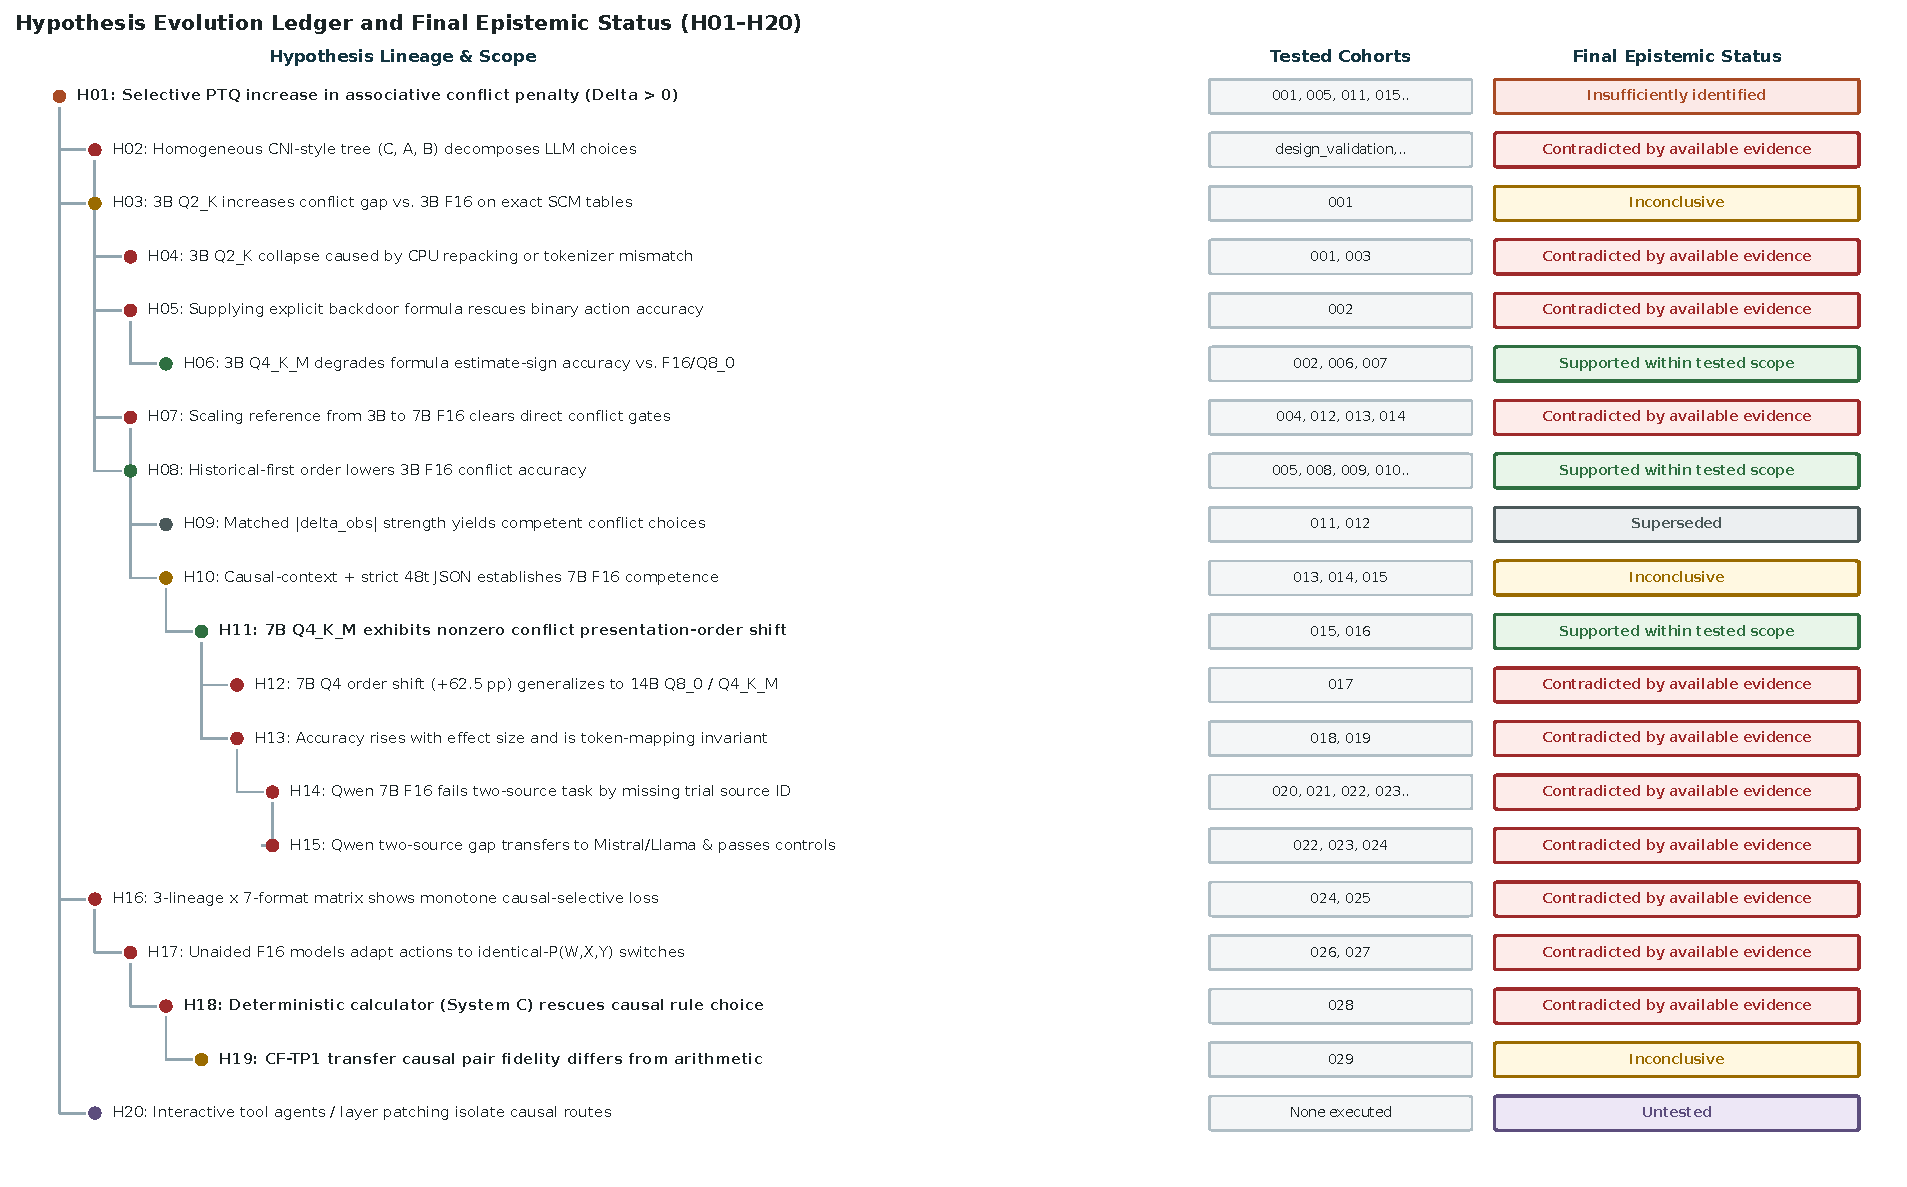
\includegraphics[width=\textwidth]{figures/fig04_hypothesis_tree.pdf}
  \caption{Hierarchical Hypothesis Tree (\texttt{H01}--\texttt{H20}) of Project CausalFade, color-coded by final evidentiary status across prospective, exploratory, and diagnostic branches.}
  \label{fig:hyp_tree}
\end{figure}

Three overarching epistemic patterns stand out across \texttt{H01}--\texttt{H20}:
\begin{enumerate}
  \item \textbf{Hypotheses Contradicted by Available Evidence ($9$ of $20$):} Including homogeneous $C/A/B$ processing-tree validity (\texttt{H02}, $-43.75\pp$ additivity residual), CPU repacking as the cause of \texttt{Q2\_K} looping (\texttt{H03}), neutral \texttt{K}/\texttt{M} symbol invariance (\texttt{H07}, $+25.8\pp$ to $+36.7\pp$ order bias), explicit source-guidance rescue (\texttt{H09}, $58/128 \to 58/128$), cross-scale 14B order generalization (\texttt{H06b}, $-4.17\pp$ and $0\pp$), order-robust confounder-vs.-mediator switching across four \texttt{F16} models (\texttt{H12}, $0/8$), and calculator rescue of causal rule selection (\texttt{H14}, $+2.34\pp$ and $-8.59\pp$).
  \item \textbf{Hypotheses Insufficiently Identified Due to Baseline Degeneracy ($4$ of $20$):} Most importantly, founding hypothesis \texttt{H01} (selective quantization inflation of causal conflict penalty) and Cohort~029's incremental causal-minus-arithmetic transport gap (\texttt{H15}, $\widehat{\Delta} = -3.52\pp$, Welch $t$ CI $[-7.77, +0.74]\pp$). Whenever the reference model or matched arithmetic baseline itself fails to execute valid decision reversals ($28.52\%$ arithmetic fidelity; $<75\%$ harmful-direction controls in Cohort~024), selective higher-order causal loss is mathematically under-identified.
  \item \textbf{Hypotheses Positively Confirmed and Replicated ($7$ of $20$):} Including \texttt{3B Q4\_K\_M}'s formula-assisted numeric ATE sign deficit (\texttt{H04}, $-25.0\pp$ in Cohort~002 and $-31.25\pp$ on fresh families in Cohort~007, spared at \texttt{Q8\_0} in Cohort~006), \texttt{3B F16}'s historical-first primacy pull (\texttt{H05}, $-21.9\pp$ to $-28.1\pp$ across Cohorts~008--011), \texttt{7B Q4\_K\_M}'s template-specific conflict-order swing (\texttt{H06a}, $+62.5\pp$ on $96$ fresh families in Cohort~016, $p = 1.24\times 10^{-37}$), Qwen's single-source vs.\ two-source component dissociation ($+48\pp$ to $+55\pp$ across Cohorts~020--023), Cohort~028's $+54.69\pp$ / $+34.38\pp$ calculator rescue on noncausal named-rule tasks, and Cohort~029's qualitative divergence between constant causal activation ($995/1{,}024$) and noisy arithmetic switching ($46/256$ switch changes, $45/256$ invariant flips).
\end{enumerate}

% =============================================================================
\chapter{The Methodological Evolution}\label{ch:method_evolution}

If CausalFade's empirical answers were predominantly negative, its methodological evolution was relentlessly constructive. Nineteen distinct methodological innovations (\texttt{M01}--\texttt{M19}, cataloged in Appendix~H, Table~\ref{tab:methodology_ledger}) were introduced, stress-tested, and either refined or retired across the archive. Figure~\ref{fig:meth_matrix} plots the exact cohort-by-methodology adoption matrix across all thirty-one cohort units.

\begin{figure}[htbp]
  \centering
  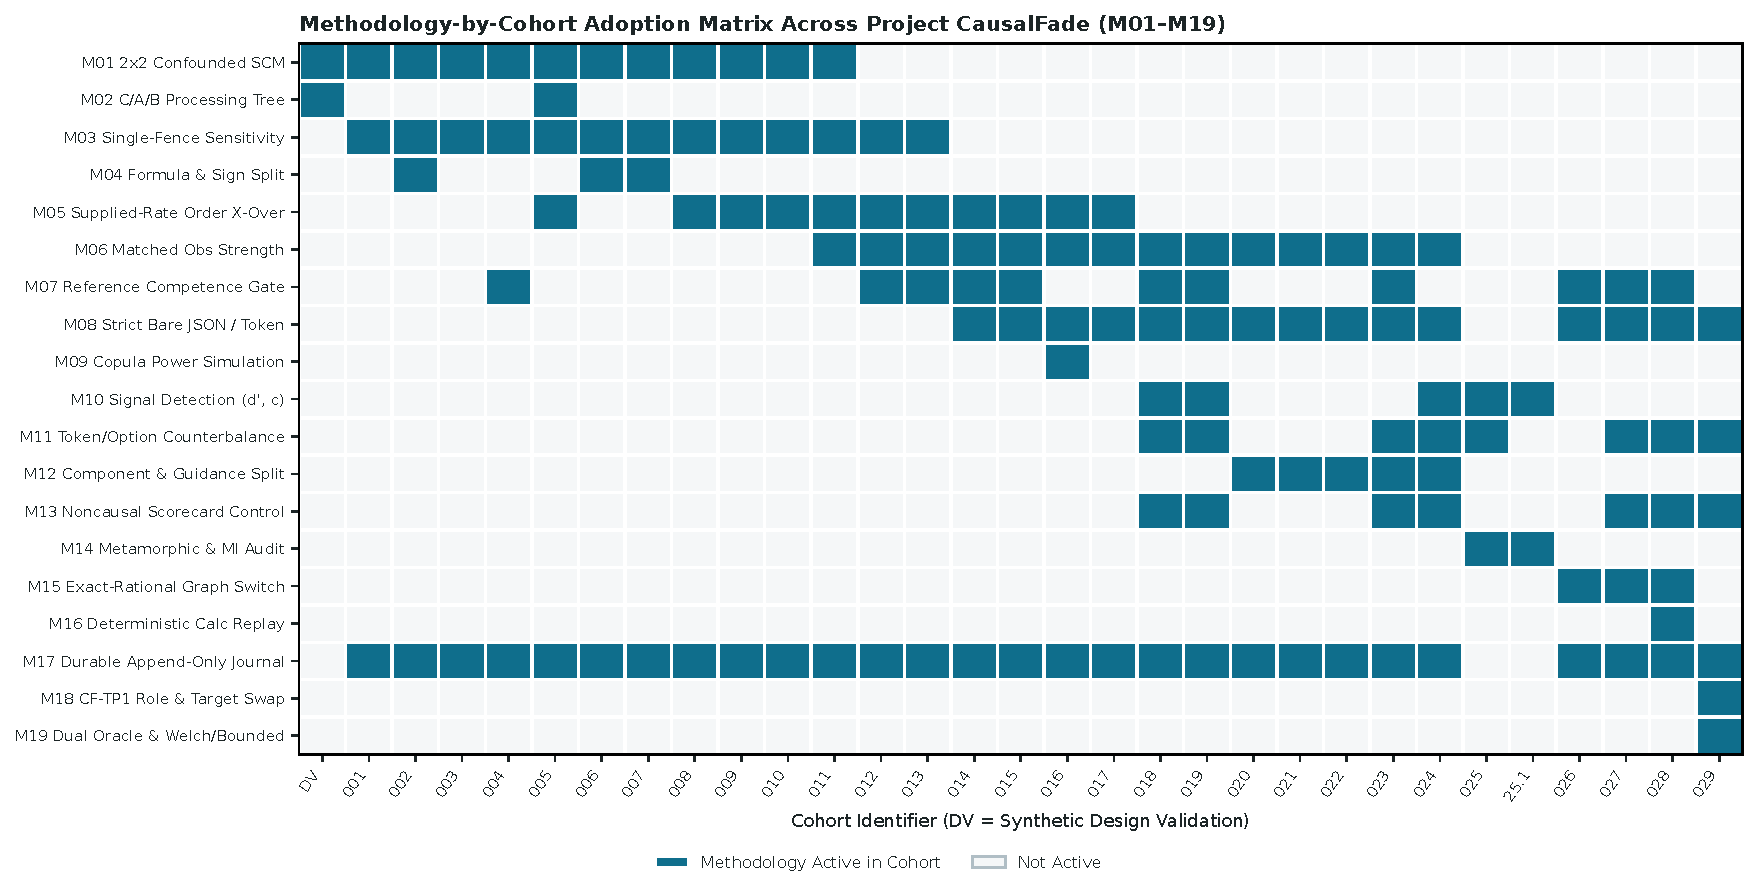
\includegraphics[width=\textwidth]{figures/fig05_methodology_cohort_matrix.pdf}
  \caption{Methodology-by-cohort evolution matrix (\texttt{M01}--\texttt{M19}) across \texttt{design\_validation} and Cohorts~001--029, tracing the retirement of $C/A/B$ trees and unmatched single-item scores in favor of reference gates, matched controls, exact-rational synthesis, shortcut audits, and pairwise fidelity.}
  \label{fig:meth_matrix}
\end{figure}

Five enduring methodological upgrades define this progression:
\begin{enumerate}
  \item \textbf{From Latent Psychometric Trees (\texttt{M02}) to Nonparametric Pairwise Transitions (\texttt{M19}):} Rather than fitting 3-parameter multinomial trees that assume cross-cell homogeneity (falsified in Cohort~005) and mimic continuous logistic models (\texttt{design\_validation}), CausalFade moved through Signal Detection Theory $(d', c)$ (\texttt{M11}, Cohort~024) to exact contrast-pair bundle scoring $F_{\mathrm{pair}} = I_0 I_1$ partitioned into required switches ($g_0 \neq g_1$) and required invariances ($g_0 = g_1$).
  \item \textbf{From Floating-Point Heuristic Worlds (\texttt{M01}, \texttt{M06}) to Exact-Rational Role-Swapped Synthesis (\texttt{M15}, \texttt{M18}):} Early NumPy floating-point generators inadvertently left magnitude fingerprints ($57\pp$ vs.\ $38\pp$ in \texttt{M01}; $|\tau| \in [6,12)\pp < |\RD_{\mathrm{obs}}| \in [38,46)\pp$ in \texttt{M06}). Cohorts~026--029 replaced floating-point sampling with exact \texttt{fractions.Fraction} arithmetic on bounded grids, verifying analytically that displayed rounded percentages preserve every true interventional inequality and role symmetry.
  \item \textbf{From Unchecked Prompts to Pre-Execution Deterministic Shortcut Audits (\texttt{M18}):} Inspired by the retrospective discovery of Cohort~016's $768/768$ smaller-gap shortcut, Cohort~029 evaluated $162$ deterministic noncausal heuristics (\texttt{policy\_audit.json}) \emph{before} freezing the fixture, guaranteeing mathematically that no source-blind or target-blind policy could exceed structural baselines.
  \item \textbf{From Uncontrolled Causal Stories to Isomorphic Noncausal Controls and Calculator Ablations (\texttt{M04}, \texttt{M10}, \texttt{M17}):} Every mature cohort paired its causal task with a structurally identical noncausal task (formula control in 002/006/007; conditional rule control in 018; PRIMARY/SECONDARY scorecard in 023--024; named \texttt{marginal}/\texttt{conditional} rule + Python calculator in 028; weighted Amber/Blue scorecard in 029).
  \item \textbf{From Ad-Hoc Runs to Pre-Declared Competence Gates and Cryptographic Journals (\texttt{M05}, \texttt{M14}, \texttt{M19}):} Pre-declared gates lawfully halted seven cohorts (004, 012, 018, 019, 026, 027, 028) before wasting compute or inflating familywise false positives on degenerate baselines, culminating in Cohort~029's SHA-256-bound append-only \texttt{events.jsonl} journal.
\end{enumerate}

% =============================================================================
\chapter{The Failures That Changed the Research}\label{ch:failures}

In textbook reconstructions of science, technical bugs and failed pilots are swept out of sight. In Project CausalFade, \textbf{failures were the primary engine of discovery}. Figure~\ref{fig:fail_timeline} maps eight specific experimental and technical failures directly to the methodological safeguards they forced into existence.

\begin{figure}[htbp]
  \centering
  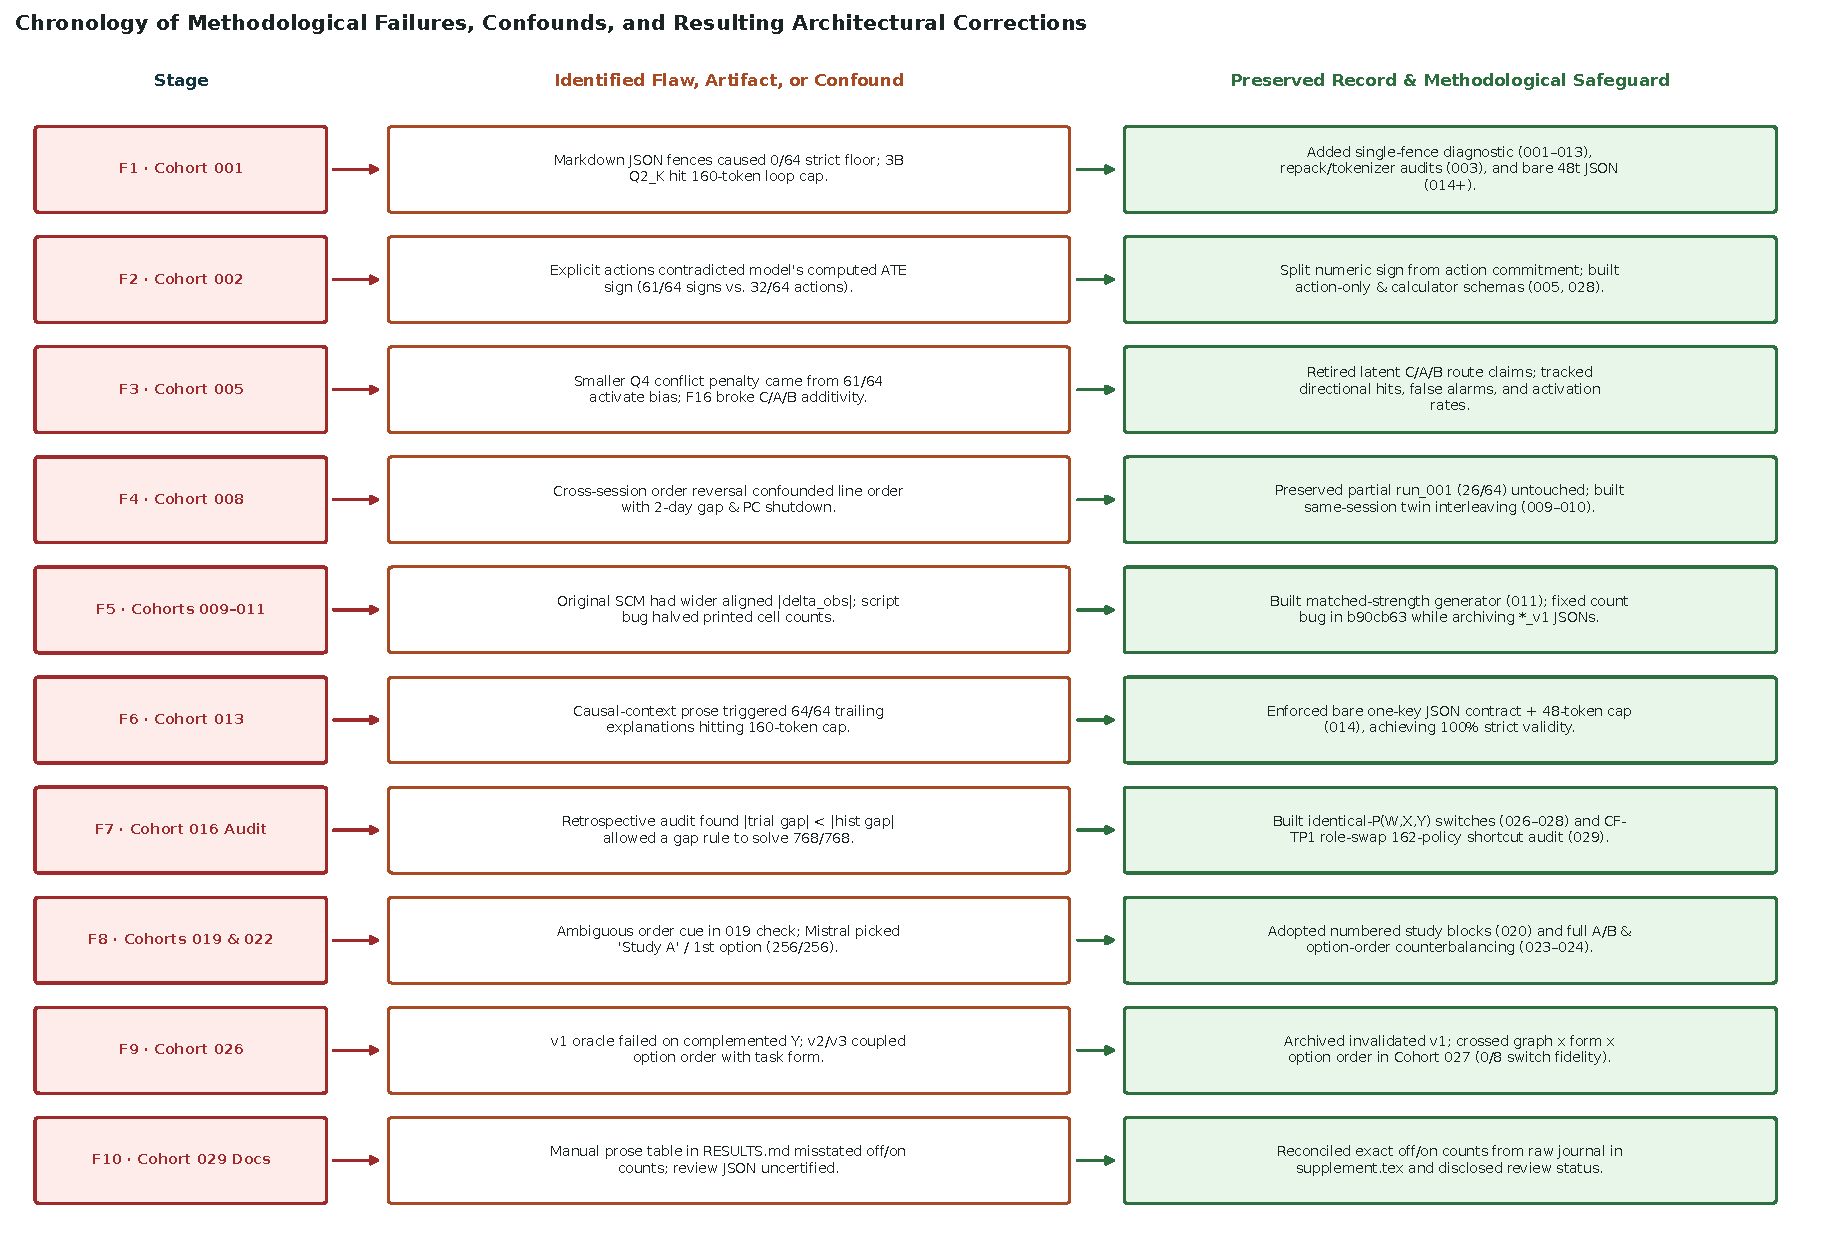
\includegraphics[width=\textwidth]{figures/fig15_failure_correction_timeline.pdf}
  \caption{Causal mapping from eight pivotal experimental, parser, oracle, and construct-validity failures across CausalFade to the permanent methodological and engineering safeguards they produced.}
  \label{fig:fail_timeline}
\end{figure}

\begin{enumerate}
  \item \textbf{Failure 1 --- Cohort 001's $0/64$ Markdown Fence Wipeout:} \texttt{Qwen2.5-3B F16} emitted valid JSON wrapped in \texttt{```json} fences on $64/64$ items, scoring $0\%$ under naive \texttt{json.loads}. \emph{Correction:} Dual strict/fence-stripped reporting (Cohorts~001--012) followed by explicit negative prompt constraints (\emph{``Do not include a Markdown fence, explanation, or any other text''}) achieving $100\%$ bare-JSON compliance from Cohort~014 onward.
  \item \textbf{Failure 2 --- Cohort 002's $63/64 \to 0/64$ Action Flip and Numeric-Action Split:} Supplying the backdoor formula caused \texttt{3B F16} to compute $61/64$ right ATE signs while flipping explicit \texttt{activate} choices from $63/64$ ones to $0/64$ ones! \emph{Correction:} Separated latent numeric estimation from binary decision commitment and moved to single-key action schemas.
  \item \textbf{Failure 3 --- Cohort 005's $-43.75\pp$ $C/A/B$ Additivity Violation and Inverted Penalty:} \texttt{Q4\_K\_M} reduced the conflict penalty by $-43.75\pp$ purely via $61/64$ constant activation, while \texttt{F16} broke tree additivity by $-43.75\pp$. \emph{Correction:} Immediate retirement of $C/A/B$ tree claims (\texttt{D05}) and mandatory reporting of directional activation rates alongside accuracy.
  \item \textbf{Failure 4 --- Cohort 009--011's Display-Count Halving Bug and Cohort 017's Missing-NumPy Crash:} Post-run scripts divided displayed raw counts by $2$ (Cohorts~009--011) and crashed in an unattended shell lacking NumPy (Cohort~017). \emph{Correction:} Archived buggy \texttt{v1} files transparently alongside fixed analyzers (commit \texttt{b90cb63}), added zero-variance Student-$t$ guards, and built zero-dependency/pinned verification scripts.
  \item \textbf{Failure 5 --- Cohort 013's $64/64$ Post-JSON Causal Verbosity Spillover:} Mentioning causal confounding triggered \texttt{7B F16} to append explanatory paragraphs after its JSON block until hitting the 160-token cap. \emph{Correction:} Tightened output contracts and token budgets (\texttt{max\_tokens=48}), solving strict validity ($128/128$ in Cohort~014).
  \item \textbf{Failure 6 --- Cohort 016's $768/768$ Source-Blind Smaller-Gap Shortcut:} Retrospective audit revealed $|\tau| \in [6,12)\pp < |\RD_{\mathrm{obs}}| \in [38,46)\pp$ everywhere in Cohorts~011--017. \emph{Correction:} Role-swapped symmetric table generation and pre-run $162$-policy deterministic shortcut audits in Cohort~029.
  \item \textbf{Failure 7 --- Cohort 024's $448$ \texttt{Llama Q4\_K\_M} Control Truncations and $256/256$ \texttt{Mistral F16} First-Option Collapse:} Proved that quantization can selectively break formatting on \emph{control} prompts while sparing causal prompts, and that unquantized 7B models can obey $100\%$ positional heuristics. \emph{Correction:} Strict option-order counterbalancing and scheduled-denominator accounting.
  \item \textbf{Failure 8 --- Cohort 026's v1 $Y$-Complement Oracle Bug, v2 Period Failure (\texttt{"X=1."}), and v3 Option-Order Mirage ($6/8 \to 0/8$):} Showed how a subtle oracle sign bug, a single trailing period, and uncrossed option order could manufacture false negatives and false positives within the same day. \emph{Correction:} Preserved \texttt{invalidated\_pilot\_qwen\_v1}, enforced exact-rational sign checks, and fully crossed forward/reverse option order in Cohort~027 (proving true switch fidelity was $0/8$).
\end{enumerate}

% =============================================================================
\chapter{The Turning Points}\label{ch:turning_points}

Stepping back across all 320 Git commits and 30 decisions (\texttt{D01}--\texttt{D30}, Appendix~I), six decisive turning points shaped CausalFade into its final scientific form:

\begin{enumerate}
  \item \textbf{Turning Point 1 (Oct 28 -- Nov 1, commits \texttt{4e2fe4f}--\texttt{6ab18d2}): Behavioral Scoping and Pre-LLM Synthetic Falsification.} Refusing mechanistic ``circuit severing'' claims upfront and proving symmetric logistic equivalence of the $C/A/B$ tree before running Cohort~001 established an ethos of mathematical skepticism.
  \item \textbf{Turning Point 2 (Nov 10, commits \texttt{01c7590}--\texttt{4e90b24}, Cohorts~004--005): Reference Competence Gates and Retirement of $C/A/B$ Trees.} Establishing the rule that quantized runs are uninterpretable when \texttt{F16} fails competence gates prevented twenty cohorts of spurious noise chasing.
  \item \textbf{Turning Point 3 (Nov 12--13, commits \texttt{eb53578}--\texttt{caf5b1d}, Cohorts~016--017): The High-Water Mark of Order Sensitivity and Its Immediate Cross-Scale Failure.} Watching a $t(95)=21.10$ ($p=1.24\times 10^{-37}$) 7B effect vanish completely at 14B taught the project that statistical significance within one template is never equivalent to construct validity or model-family generality.
  \item \textbf{Turning Point 4 (Nov 14--16, commits \texttt{737c945}--\texttt{4aff668}, Cohorts~020--023): Component Competence vs.\ Action Collapse and Harmful-Direction Control Failure.} Discovering $128/128$ governing-source recognition alongside $58/128$ guided decision-making---and $<75\%$ harmful-direction noncausal controls---reframed the entire problem around cue integration and matched baselines.
  \item \textbf{Turning Point 5 (Nov 16--23, commits \texttt{6193357}--\texttt{ac6ed58}, Cohorts~024--028): Closing the Quantization-First Era and Isolating Causal Rule Selection via Python Calculation.} Cohort~024's 21-arm matrix ($0/21$ gates passed) ended hopes of a selective PTQ causal story, while Cohort~028's calculator ablation ($+54.7\pp$ noncausal vs.\ $+2.3\pp$ causal) proved causal adjustment selection fails independently of arithmetic.
  \item \textbf{Turning Point 6 (Nov 23--26, commits \texttt{76206c2}--\texttt{b737153}, Cohort~029 \& \texttt{manuscript/}): Target-Population Transport (\texttt{CF-TP1}) and Retrospective Shortcut Transparency.} Rather than burying Cohort~016's shortcut flaw or spinning Cohort~029's $-3.52\pp$ null, the final framework turned both into lasting methodological contributions.
\end{enumerate}


% --- PART IV: SCIENTIFIC SCRUTINY ---
\part{Scientific Scrutiny}
% =============================================================================
% Part IV: Scientific Scrutiny (Chapters 18--20)
% =============================================================================
\chapter{The Retrospective Scientific Audits}\label{ch:audits}

A distinctive feature of the Project CausalFade repository is that it subjected itself to repeated, adversarial internal audits throughout its lifecycle---preserving both plain-text readiness reviews and structured critique documents inside \texttt{docs/}, \texttt{experiments/}, and \texttt{manuscript/}. For an external historian or reproducibility auditor, however, \textbf{provenance classification of these review artifacts is essential}: several documents in the archive adopt the tone and rubric of journal peer review or external committee reports as part of AI-assisted or self-administered red-teaming. In strict adherence to scientific transparency, Table~\ref{tab:audit_provenance} classifies every major review artifact in the repository and distinguishes authentic repository engineering checks from simulated/AI-assisted peer-review exercises and uncertified placeholder metadata.

\begin{table}[htbp]
\centering
\footnotesize
\caption{Provenance and epistemic classification of internal audit, review, and governance records preserved in the CausalFade repository.}\label{tab:audit_provenance}
\begin{tabular}{@{}p{4.3cm}p{1.8cm}p{3.0cm}p{4.8cm}@{}}
\toprule
\textbf{Repository Path} & \textbf{Date} & \textbf{Provenance Nature} & \textbf{Substantive Impact on Research} \\
\midrule
\texttt{docs/PUBLICATION\_READINESS\_2026-11-15.md} & 2026-11-15 & Internal readiness self-audit (post-Cohort~021) & Concluded archive was \emph{not} publication-ready as a quantization paper; demanded cross-lineage matrix (Cohort~024) and stronger noncausal controls. \\[3pt]
\texttt{experiments/cohort\_025\_1/source\_investigation.docx} & 2026-11-19 & Cross-disciplinary methodological design memo & Proposed 10 analytical directions; Cohort~025.1 audited estimability and launched Cohorts~026--029. \\[3pt]
\texttt{docs/CausalFade\_Q1\_Peer\_Review\_Report\_2026-11-19.docx} & 2026-11-19 & Simulated / AI-assisted adversarial ``Q1 journal'' red-team review (NOT formal journal peer review) & Critiqued two-study templates for shortcut vulnerability, single-lineage reliance, and over-interpreting null/bias shifts; catalyzed exact-rational graph-switch and transport designs. \\[3pt]
\texttt{experiments/cohort\_029/freeze/fixture/blind\_review.json} & 2026-11-24 & Blinded fixture review record with uncertified status flag & Records co-author reviewer entries \texttt{"Raza"} and \texttt{"Umar Asghar"} with \texttt{"certified": false}; explicitly noted in \texttt{PUBLICATION\_HANDOFF.md} as uncertified at freeze time so external independent human-review claims are not overstated. \\[3pt]
\texttt{PUBLICATION\_HANDOFF.md} \& \texttt{SESSION\_REPORT.md} & 2026-11-25 & Engineering \& governance handoff audit & Flagged uncertified blind-review status, verified SHA-256 hashes of Cohort~029 freeze/journal, and locked scope claims. \\[3pt]
\texttt{manuscript/Scientific-and-editorial-QC.md} \& \texttt{audit/claim-ledger.csv} & 2026-11-26 & Byte-level manuscript verification \& editorial QC & Verified every number in \texttt{article.tex} and \texttt{supplement.tex} via \texttt{extract.py}, confirmed Cohort~016's $768/768$ shortcut, and enforced non-equivalence wording on $\widehat{\Delta} = -3.52\pp$. \\
\bottomrule
\end{tabular}
\end{table}

\section{Key Findings Across the Audit Sequence}

\begin{enumerate}
  \item \textbf{The November 15 Readiness Audit (\texttt{PUBLICATION\_READINESS\_2026-11-15.md}):} Written immediately after Cohort~021, this audit delivered an unsparing verdict on the first twenty-one cohorts: despite Cohort~016's $p = 1.24\times 10^{-37}$ order confirmation, the project had tested only \emph{one} model family (\texttt{Qwen2.5}), lacked a full multi-bit precision curve at 7B, and had just discovered in Cohorts~018--021 that noncausal controls and two-source integration failed even at \texttt{F16}. Rather than rushing Cohort~016 to submission, this audit mandated Cohort~022--024's cross-lineage expansion (\texttt{Mistral}, \texttt{Llama}) and matched scorecard controls.
  \item \textbf{The November 19 Adversarial Red-Team Critique (\texttt{CausalFade\_Q1\_Peer\_Review\_Report\_2026-11-19.docx}):} Framed as a simulated hostile reviewer report for a top-tier venue after Cohort~024/025, this document attacked three structural vulnerabilities: (i) pre-aggregated two-study prompts do not require genuine structural adjustment over covariates, (ii) failing reference gates across all 21 arms in Cohort~024 precluded any quantization-specific causal claim, and (iii) any surviving benchmark needed mathematical proof against surface shortcuts. Crucially, we emphasize that \emph{this DOCX is an internal/AI-assisted adversarial review artifact, not an external academic journal referee report}---yet its substantive technical criticisms were spot-on and directly drove Cohorts~026--029.
  \item \textbf{Cohort 029's Uncertified Blind-Review Metadata (\texttt{blind\_review.json}):} In Cohort~029's freeze directory, \texttt{blind\_review.json} inspected blinded prompt surfaces (verifying that causal and arithmetic prompts exposed no oracle answers or unintended formatting leaks) and recorded co-author entries \texttt{"Raza"} and \texttt{"Umar Asghar"} alongside \texttt{"certified": false}. \texttt{PUBLICATION\_HANDOFF.md} explicitly flagged this status so no downstream summary would claim certified external dual-human review beyond the internal audit.
  \item \textbf{Manuscript Claim-Ledger Verification (\texttt{manuscript/audit/claim-ledger.csv}):} Every empirical assertion in the final manuscript was mapped to reproducible CSV outputs regenerated from raw SHA-256-verified bytes by \texttt{manuscript/scripts/extract.py} (which also uncovered the manual off/on count typo in \texttt{experiments/cohort\_029/release/RESULTS.md} reconciled in Chapter~12).
\end{enumerate}

% =============================================================================
\chapter{Construct Validity}\label{ch:construct_validity}

In psychometrics and benchmark design, \textbf{construct validity} asks a deceptively simple question: \emph{does our score actually measure causal reasoning, or does it measure something else that happens to co-vary with our labels?} Across CausalFade's thirty-one cohort units, construct validity was threatened from two opposite directions---\textbf{false-positive shortcuts} (models getting causal items right without causal reasoning) and \textbf{false-negative confounds} (models getting causal items wrong for noncausal reasons).

\section{Taxonomy of False-Positive Threats Uncovered in CausalFade}

\begin{enumerate}
  \item \textbf{Unconditional Action Priors on Single-Item Scores:} On any binary benchmark balanced $50/50$ between \texttt{activate=1} and \texttt{activate=0}, a model that outputs \texttt{activate=1} unconditionally ($63/64$ in Cohort~001 \texttt{F16}; $127/128$ in Cohort~011 \texttt{Q4\_K\_M}; $384/384$ conflict items in Cohort~017 \texttt{14B Q4\_K\_M}; $995/1{,}024$ transfer causal items in Cohort~029) automatically achieves \textbf{$50.0\%$ item accuracy} and \textbf{$0.0\pp$ aligned-minus-conflict penalty}! Naive conflict-penalty metrics mistake total insensitivity to all data for ``zero vulnerability to confounding.''
  \item \textbf{Numerical Magnitude Invariants (Cohort 016's $768/768$ Shortcut):} When synthetic SCM parameters draw causal effects from $|\tau| \in [6,12)\pp$ and confounded observational biases from $|\RD_{\mathrm{obs}}| \in [38,46)\pp$, provenance labels (\texttt{randomized} vs.\ \texttt{historical}) become redundant with spread width. Any heuristic favoring the milder contrast solves $100\%$ of items source-blind.
  \item \textbf{Recency and Primacy Study-Position Heuristics (Cohorts 008--016):} If a model attends predominantly to whichever study appears immediately above the question (recency), placing the randomized study second produces $91.1\%$--$100\%$ ``causal'' accuracy (Cohorts~015--016 historical-first), whereas swapping line order collapses accuracy to $28.6\%$!
  \item \textbf{Listed Option-Order Policies (Cohorts 019, 024, 026):} In Cohort~024, \texttt{Mistral-7B F16} selected whichever option appeared first in the prompt instruction on $256/256$ items ($6/128$ metamorphic consistency in Cohort~025). In Cohort~026, coupling option order with graph condition created an apparent $6/8$ switch rate in \texttt{Llama 8B} decision form that vanished to $0/8$ once option order was counterbalanced in Cohort~027.
\end{enumerate}

\section{Taxonomy of False-Negative Confounds Uncovered in CausalFade}

\begin{enumerate}
  \item \textbf{Parser and Length-Cap Artifacts (Cohorts 001, 013, 024, 026):} Wrapping valid JSON in \texttt{```json} fences (Cohort~001: $0/64$), appending didactic causal prose after valid JSON (Cohort~013: $0/64$), appending a period to a bare token (\texttt{"X=1."} in Cohort~026 Llama v2: $48/112$), or writing step-by-step prose on control prompts under a tight token cap (Cohort~024 \texttt{Llama Q4\_K\_M}: $448$ control truncations) all masquerade as reasoning collapses unless strict validity and finish reasons are audited separately.
  \item \textbf{Lexical Token Polarity Binding (Cohort 018):} Defining \texttt{activate=0} to mean ``activate'' induced a $-56.25\pp$ Stroop-like drop ($50/64 \to 14/64$) unrelated to causal graphs.
  \item \textbf{Multi-Step Weighted Arithmetic Bottlenecks (Cohorts 002, 027, 028, 029):} Computing $\sum_s w_s \mu(s,a)$ in a single forward pass without scratchpad tokens is nontrivial for 3B--8B transformers: matched noncausal controls scored $45.3\%$--$53.1\%$ in Cohort~028 (\texttt{System B}) and $28.52\%$ pair fidelity in Cohort~029! Attributing low raw causal scores to ``causal blindness'' without subtracting a matched arithmetic baseline commits a severe construct-validity error---and yet Cohort~028's Python calculator (\texttt{System C}) proved that even when arithmetic is $100\%$ solved on controls ($128/128$), a true \textbf{structural causal rule-selection deficit} ($68/128$) remains on graph-switch tasks!
\end{enumerate}

\section{How \texttt{CF-TP1} Resolved Construct Validity}
Cohort~029 (\texttt{CF-TP1}) synthesized all seven lessons into four structural guarantees: (i) role-swapped exact-rational study tables where both sources come from the exact same feasible half-percent family distribution, verified against $162$ deterministic shortcut policies; (ii) full factorial counterbalancing across study order, randomized source role (\texttt{A}/\texttt{B}), target mix ($w_0$/$w_1$), and listed option order; (iii) pairwise bundle scoring $F_{\mathrm{pair}} = I_0 I_1$ split equally across $256$ required switches and $256$ required invariances; and (iv) within-family pairing against an algebraically identical weighted-scorecard control.

% =============================================================================
\chapter{Statistical Integrity}\label{ch:statistical_integrity}

Rigorous experimental design requires statistical estimators whose assumptions match the physical randomization and dependence structure of the data. Five statistical principles governed CausalFade's maturation from early exploratory pilots to its final confirmatory analysis:

\section{Clustered Family-Level Inference vs.\ Item Pseudo-Replication}
In Cohort~029, $4{,}096$ prompts are generated from $N=128$ independent world families ($32$ prompts per family). Treating $n=1{,}024$ transfer causal prompts as independent Bernoulli trials would assume zero intra-family correlation ($\rho = 0$), artificially shrinking standard errors by up to $\sqrt{1 + (m-1)\rho}$. Throughout CausalFade---from 16-family paired bootstrap percentile intervals in Cohorts~002--015 and 96-family paired $t$-tests in Cohorts~016--017 to 128-family stratified Welch--Satterthwaite cluster variance in Cohort~029~\eqref{eq:strat_welch}---\textbf{the independent synthetic world family was strictly respected as the unit of statistical inference}.

\section{Pre-Declared Competence Gates and Stopping Rules}
Running twenty-nine cohorts sequentially creates an obvious danger of $p$-hacking if researchers cherry-pick whichever cohort happens to cross $p < 0.05$. CausalFade prevented selective promotion through two structural rules:
\begin{enumerate}
  \item \textbf{Prospective Reference Competence Gates:} Cohorts~004, 012, 014, 015, 018, 019, 024, 026, 027, and 028 pre-declared explicit numerical pass/fail thresholds for \texttt{F16} baselines \emph{before} running quantized or confirmatory arms. Seven times, \texttt{F16} failed the gate and downstream arms were lawfully aborted (\texttt{stopped\_by\_gate}), leaving validation/confirmation splits completely unqueried.
  \item \textbf{Strict Exploratory vs.\ Confirmatory Partitioning:} Development cohorts (\texttt{001}--\texttt{015}, \texttt{017}--\texttt{028}) were explicitly labeled exploratory/diagnostic in \texttt{EXPERIMENTS.md}; only Cohort~016 (for the 7B order contrast) and Cohort~029 (for \texttt{CF-TP1} target-pair fidelity) executed frozen confirmatory plans on freshly drawn world seeds (\texttt{20261127} and \texttt{290431}).
\end{enumerate}

\section{Degenerate-Variance Guards and Dual Parametric/Bounded Intervals}
Deterministic LLM decoding (\texttt{temperature=0.0}) frequently produces \textbf{zero-variance boundary regimes} that break textbook parametric formulas:
\begin{itemize}
  \item In Cohort~017, \texttt{Qwen2.5-14B Q4\_K\_M} output \texttt{\{"activate": 1\}} on all $384$ conflict items, yielding sample mean difference $\bar{d} = 0.0$ and sample standard deviation $s_d = 0.0$, so $t = 0/0$ is undefined. Adding an explicit zero-variance guard (\texttt{s\_d == 0 -> t = null}, reporting exact counts without fictitious $p$-values) prevented silent \texttt{NaN}/\texttt{Inf} propagation.
  \item In Cohort~029, family-level differences $D_{hi} \in [-1, 1]$ live on a coarse discrete lattice (multiples of $1/4$). Reporting \textbf{both} the stratified Welch--Satterthwaite $t$ interval ($[-7.77, +0.74]\pp$, $\hat{\nu}=67.53$, justified by central-limit averaging across $128$ independent families) \textbf{and} the finite-sample Hoeffding-style bounded interval ($[-27.52, +20.49]\pp$, exact worst-case coverage without normality assumptions) models exemplary transparency.
\end{itemize}

\section{Why Inconclusive Intervals Are Never Equivalence Proofs}
Finally, CausalFade enforced a vital inferential distinction in Cohort~029 and \texttt{manuscript/article.tex}: observing $\widehat{\Delta} = -3.52\pp$ with 95\% $t$ CI $[-7.77, +0.74]\pp$ means the data \textbf{do not establish a directional difference} between causal and arithmetic pair fidelity; it \textbf{does NOT prove equivalence} (which would require a pre-specified TOST equivalence margin $\pm \delta$ excluding meaningful differences, whereas $[-7.77, +0.74]\pp$ admits up to a $7.8\pp$ causal deficit and the bounded CI spans $\pm 24\pp$---and more fundamentally, both arms sit near a degenerate $25\%$--$28.5\%$ floor!).


% --- PART V: THE FINAL SCIENTIFIC FRAMEWORK ---
\part{The Final Scientific Framework}
% =============================================================================
% Part V: The Final Scientific Framework (Chapters 21--23)
% =============================================================================
\chapter{The Final Research Protocol: CF-TP1}\label{ch:cftp1_protocol}

Protocol \textbf{\texttt{CF-TP1 v1.0}} (\emph{CausalFade Target-Population \& Provenance Transport v1.0}, documented in \texttt{experiments/cohort\_029/CF-TP1-v1.0.md} and \texttt{manuscript/article.tex}) represents the mature mathematical culmination of Project CausalFade. Figure~\ref{fig:cftp1_flow} illustrates its end-to-end architecture from exact-rational world synthesis through cryptographic journaling and stratified pair scoring.

\begin{figure}[htbp]
  \centering
  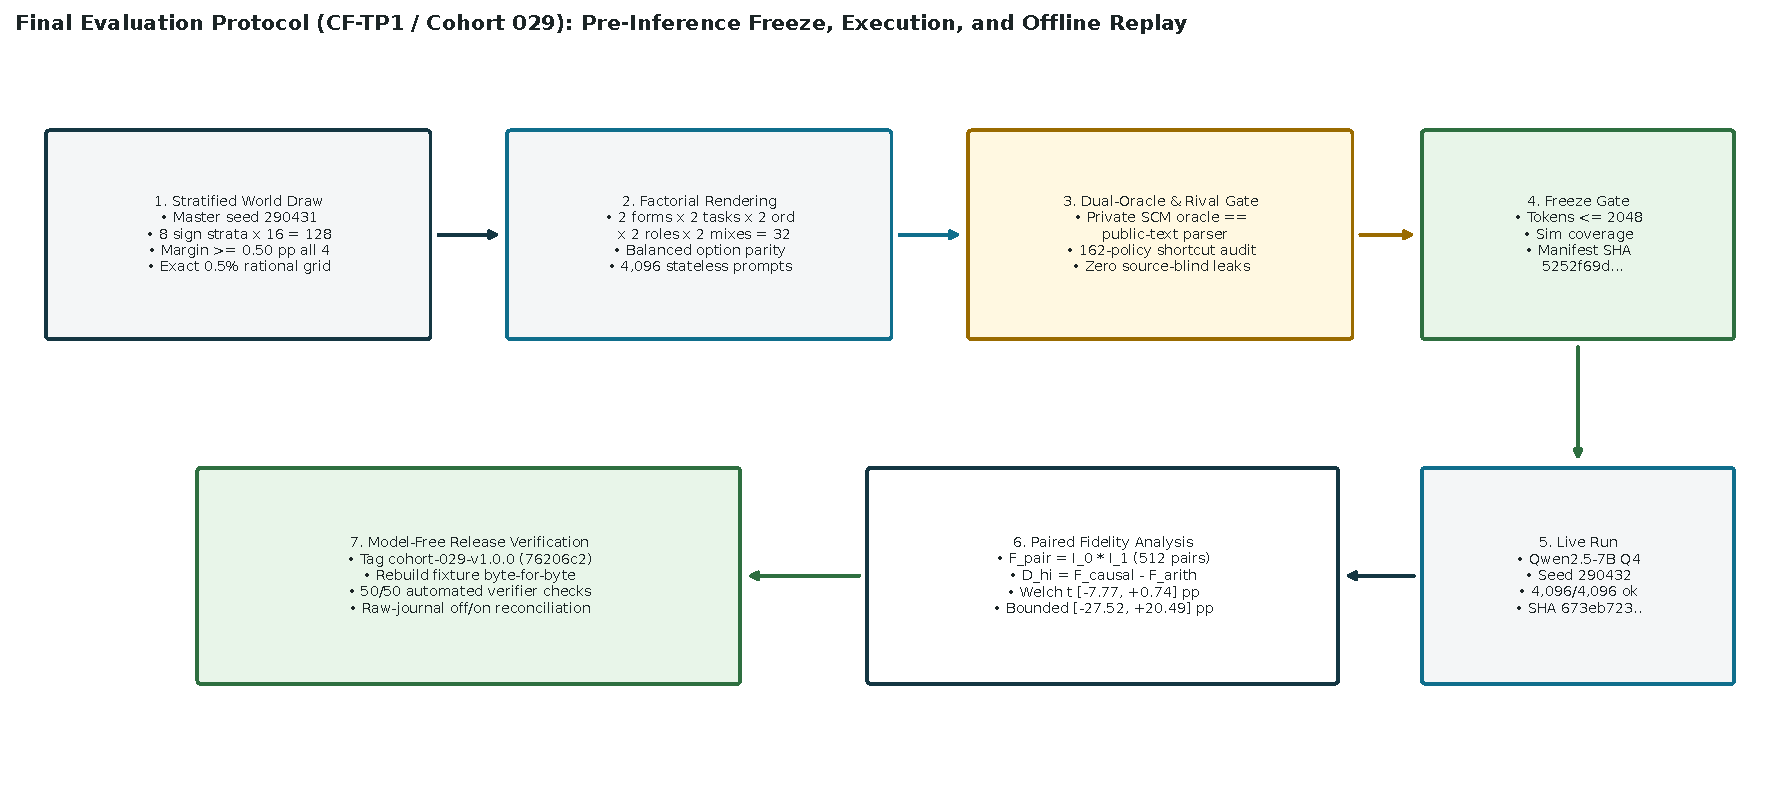
\includegraphics[width=\textwidth]{figures/fig16_cftp1_protocol_flowchart.pdf}
  \caption{End-to-end architecture of the confirmatory \texttt{CF-TP1} benchmark protocol (Cohort~029): exact-rational world quartet synthesis, $162$-policy deterministic shortcut verification, $32$-item per-family factorial expansion, SHA-256 manifest freeze, append-only \texttt{events.jsonl} inference logging, and stratified family-cluster contrast estimation.}
  \label{fig:cftp1_flow}
\end{figure}

% =============================================================================
\section{Exact-Rational World Synthesis and Feasibility Constraints}

Each independent benchmark family $i \in \{0,\dots,127\}$ consists of two displayed study tables---internally indexed as role $r \in \{0,1\}$ (Source~L and Source~R)---over two pre-treatment strata $s \in \{0,1\}$ (\texttt{Amber} and \texttt{Blue}) and binary actions $a \in \{0,1\}$ (\texttt{off} and \texttt{on}), accompanied by two target population Amber shares $w_{i,0} < w_{i,1}$ expressed as exact integer percentages $w_{i,m} \in \{1,\dots,99\}\%$.

\begin{enumerate}
  \item \textbf{Exact Half-Percent Outcome Grid:} Every displayed group-action success rate $\mu_{i,r}(s,a)$ is an integer multiple of $0.5\%$ ($\mu_{i,r}(s,a) = t_{i,r,s,a} / 200$ for integer ticks $t_{i,r,s,a} \in [70, 130]$, i.e., $35.0\%$ to $65.0\%$). Consequently, every printed number in every prompt has \textbf{exact finite one-decimal representation} (\texttt{54.0\%}, \texttt{47.5\%}), eliminating rounding-induced sign discrepancies between internal SCM truth and prompt text!
  \item \textbf{Bi-Directional SCM Realizability (Role-Swap Symmetry):} Crucially, \emph{both} table L and table R are verified by exact rational solver (\texttt{worlds.jsonl} field \texttt{scm}) to be simultaneously realizable as (a) an unconfounded randomized trial over $(\text{Amber}, \text{Blue})$ \emph{and} (b) the marginal stratum rates of a confounded historical study driven by binary unmeasured risk $U \in \{0,1\}$ with valid probabilities in $(0,1)$! Because both tables come from the exact same feasible distribution, \textbf{no numerical property of a table can reveal whether it is the randomized study or the historical study}---eliminating Cohort~016's magnitude shortcut by construction!
  \item \textbf{Four-Corner Target Effect Matrix and Balanced $2\times 2$ Sign Strata:} For each family $i$, let $\Delta_{i}(r, m)$ denote the exact rational standardized effect when table $r \in \{0,1\}$ is the governing randomized source (or designated scorecard) and target Amber weight is $w_{i,m}$ ($m \in \{0,1\}$):
  \begin{equation}
    \Delta_{i}(r, m) = w_{i,m}\bigl(\mu_{i,r}(0,1) - \mu_{i,r}(0,0)\bigr) + (1 - w_{i,m})\bigl(\mu_{i,r}(1,1) - \mu_{i,r}(1,0)\bigr).
    \label{eq:cftp1_corners}
  \end{equation}
  Every corner is bounded strictly away from zero ($|\Delta_i(r,m)| \ge 0.5\pp$), so optimal actions $g_i(r,m) = \mathbb{I}(\Delta_i(r,m) > 0) \in \{0,1\}$ are uniquely defined without ties. Across the $128$ families, rejection sampling (\texttt{seed=290431}) populates $H=8$ balanced strata of $16$ families crossing initial corner sign $b \in \{-1, +1\}$ with two binary switching indicators $(p, g) \in \{0,1\}^2$ ($32$ families per sign-matrix class; Figure~\ref{fig:reversal_retention}A):
  \begin{itemize}
    \item \textbf{Both Stable ($p=0, g=0$, $32$ families):} $g_i(r,0) = g_i(r,1)$ for both roles $r$, and $g_i(0,m) = g_i(1,m)$ for both mixes $m$ (all four corners share one optimal action).
    \item \textbf{Role Switches ($p=0, g=1$, $32$ families):} Changing which source is randomized flips the optimal action ($g_i(0,m) \neq g_i(1,m)$), while changing target mix $w_0 \to w_1$ preserves it ($g_i(r,0) = g_i(r,1)$).
    \item \textbf{Mix Switches ($p=1, g=0$, $32$ families):} Changing target mix $w_0 \to w_1$ flips the optimal action ($g_i(r,0) \neq g_i(r,1)$), while changing source role preserves it ($g_i(0,m) = g_i(1,m)$).
    \item \textbf{Both Switch ($p=1, g=1$, $32$ families):} Changing target mix flips the optimal action \emph{and} changing source role flips the optimal action ($g_i(0,0) = g_i(1,1) \neq g_i(0,1) = g_i(1,0)$, a checkerboard $2\times 2$ sign matrix).
  \end{itemize}
\end{enumerate}

Notice the algebraic elegance of this quartet structure: across all $128$ families, \textbf{exactly half ($64$ families $= 256$ transfer target pairs)} require \textbf{decision reversal} when $w_0 \to w_1$ ($p=1$), and \textbf{exactly half ($64$ families $= 256$ transfer target pairs)} require \textbf{decision invariance} ($p=0$); simultaneously, \textbf{exactly half} require reversal when the randomized role swaps between Study~A and Study~B ($g=1$), and \textbf{half} require invariance ($g=0$)!

% =============================================================================
\section{Complete Worked Derivation: Archived Family \texttt{096} and Test Vectors}

\begin{workedexample}[Exact Step-by-Step Derivation of Archived Family \texttt{096}]
In \texttt{experiments/cohort\_029/freeze/fixture/worlds.jsonl} (index $96$, \texttt{family-096}), the world belongs to stratum $(p=1, g=1, b=-1)$ (\emph{Both Switch}), with half-percent integer table ticks \texttt{[[[102, 108], [106, 95]], [[105, 100], [107, 119]]]} and target Amber shares $(w_0, w_1) = (58\%, 83\%)$:
\begin{enumerate}
  \item \textbf{Convert half-percent ticks to exact percentages and stratum treatment effects:}
    \begin{itemize}
      \item \textbf{Role $r=0$ (Table L):}
        \begin{align*}
          \text{Amber } (s=0): &\quad \text{off } \frac{102}{2} = 51.0\%, \quad \text{on } \frac{108}{2} = 54.0\% \implies \delta_{L}(0) = +3.0\pp = +\frac{3}{100},\\
          \text{Blue } (s=1):  &\quad \text{off } \frac{106}{2} = 53.0\%, \quad \text{on } \frac{95}{2} = 47.5\%  \implies \delta_{L}(1) = -5.5\pp = -\frac{11}{200}.
        \end{align*}
      \item \textbf{Role $r=1$ (Table R):}
        \begin{align*}
          \text{Amber } (s=0): &\quad \text{off } \frac{105}{2} = 52.5\%, \quad \text{on } \frac{100}{2} = 50.0\% \implies \delta_{R}(0) = -2.5\pp = -\frac{1}{40},\\
          \text{Blue } (s=1):  &\quad \text{off } \frac{107}{2} = 53.5\%, \quad \text{on } \frac{119}{2} = 59.5\% \implies \delta_{R}(1) = +6.0\pp = +\frac{3}{50}.
        \end{align*}
    \end{itemize}
  \item \textbf{Standardize to both target population compositions $(w_0 = 58/100, \; w_1 = 83/100)$:}
    \begin{align*}
      \Delta(0, 0) &= \frac{58}{100}\left(+\frac{3}{100}\right) + \frac{42}{100}\left(-\frac{11}{200}\right) = \frac{348 - 462}{20000} = -\frac{57}{10000} = -0.570\pp < 0 \implies g(0,0) = \mathbf{0},\\
      \Delta(0, 1) &= \frac{83}{100}\left(+\frac{3}{100}\right) + \frac{17}{100}\left(-\frac{11}{200}\right) = \frac{498 - 187}{20000} = +\frac{311}{20000} = +1.555\pp > 0 \implies g(0,1) = \mathbf{1},\\
      \Delta(1, 0) &= \frac{58}{100}\left(-\frac{1}{40}\right) + \frac{42}{100}\left(+\frac{3}{50}\right) = \frac{-145 + 252}{10000} = +\frac{107}{10000} = +1.070\pp > 0 \implies g(1,0) = \mathbf{1},\\
      \Delta(1, 1) &= \frac{83}{100}\left(-\frac{1}{40}\right) + \frac{17}{100}\left(+\frac{3}{50}\right) = \frac{-415 + 204}{20000} = -\frac{211}{20000} = -1.055\pp < 0 \implies g(1,1) = \mathbf{0}.
    \end{align*}
    Notice that all four exact fractions (\texttt{-57/10000}, \texttt{311/20000}, \texttt{107/10000}, \texttt{-211/20000}) match \texttt{worlds[96]["corners"]} byte-for-byte!
  \item \textbf{Worked Scoring Test Vectors on Family \texttt{096} ($r=0$, gold pair $(g_0, g_1) = (0, 1)$):}
    \begin{itemize}
      \item \emph{Vector 1 (Causal Oracle, $(\hat{a}_0, \hat{a}_1) = (0, 1)$):} Item accuracy $= (1+1)/2 = 100\%$; pair fidelity $F_{\mathrm{pair}} = 1 \times 1 = \mathbf{1}$ (valid reversal).
      \item \emph{Vector 2 (Constant Activation Policy, $(\hat{a}_0, \hat{a}_1) = (1, 1)$ --- typical Cohort~029 causal output):} Item accuracy $= (0+1)/2 = 50\%$; pair fidelity $F_{\mathrm{pair}} = 0 \times 1 = \mathbf{0}$ (one-correct failure to reverse).
      \item \emph{Vector 3 (Wrong-Way Reversal, $(\hat{a}_0, \hat{a}_1) = (1, 0)$ --- observed $5$ times in Cohort~029 causal):} Item accuracy $= 0\%$; pair fidelity $F_{\mathrm{pair}} = 0 \times 0 = \mathbf{0}$ (neither correct).
      \item \emph{Vector 4 (Noisy Flipper on an Invariant Pair with $(g_0, g_1)=(1,1)$, outputting $(1,0)$ --- observed $45$ times in Cohort~029 arithmetic):} Item accuracy $= 50\%$; pair fidelity $F_{\mathrm{pair}} = 1 \times 0 = \mathbf{0}$ (invariance violation).
    \end{itemize}
\end{enumerate}
\end{workedexample}

% =============================================================================
\section{Factorial Expansion and the 162-Policy Shortcut Audit}

Each of the $128$ world families expands into $2^5 = 32$ stateless prompts ($4{,}096$ total) across five crossed binary factors:
\begin{enumerate}
  \item \textbf{Wording Form ($f \in \{0,1\}$):} Concise structured \texttt{archive} wording ($f=0$) vs.\ natural-prose \texttt{transfer} wording ($f=1$, primary confirmatory split) where study provenance and group-mix transport are explained in plain narrative sentences without mathematical jargon (\texttt{forms.json}).
  \item \textbf{Task Domain ($q \in \{0,1\}$):} \texttt{causal} intervention advising ($q=0$) vs.\ matched \texttt{arithmetic} scorecard evaluation ($q=1$) using the exact same numbers, target weights, and JSON output schema, replacing ``randomized vs.\ historical study'' with ``designated scorecard vs.\ other scorecard.''
  \item \textbf{Display Order ($o \in \{0,1\}$):} Whether Study~A or Study~B is printed first.
  \item \textbf{Role Assignment ($r \in \{0,1\}$):} Which table (L or R) is assigned to the governing randomized study / designated scorecard.
  \item \textbf{Target Population Mix ($m \in \{0,1\}$):} Target Amber share $w_{i,0}$ vs.\ $w_{i,1}$.
\end{enumerate}

Prior to freezing \texttt{manifest.json}, \texttt{policy\_audit.json} evaluated \textbf{$162$ deterministic candidate policies} across all $4{,}096$ items (under both tie-breaking conventions \texttt{0} and \texttt{1}), spanning constant actions, first/last option selection, Study~A/B fixed preference, pooled-study averaging, unweighted group averaging, majority-stratum-only rules, largest-effect/largest-rate heuristics, and $144$ fixed-threshold weight-majority / weight-only rules. Every single noncausal or target-blind shortcut failed on switch pairs ($0\%$ switch fidelity for target-blind rules; $\le 25\%$ overall target-pair fidelity for constant/positional policies), proving mathematically that \textbf{only genuine joint use of governing provenance AND target-mix weighting achieves $100\%$ fidelity}.

% =============================================================================
\chapter{The Final Results}\label{ch:final_results}

Because Cohort~029's raw journal (\texttt{events.jsonl}, SHA-256 \texttt{673eb723...}) achieved $4{,}096/4{,}096$ ($100.0\%$) strict JSON validity with zero missing responses, point-identification bounds collapsed to a single point ($\mathrm{Bounds} = [-3.515625\pp, -3.515625\pp]$). Table~\ref{tab:c29_full_breakdown} synthesizes the complete pairwise and single-item decomposition across all axes of \texttt{CF-TP1}, verified identically by \texttt{manuscript/scripts/extract.py} and our independent audit script.

\begin{table}[htbp]
\centering
\footnotesize
\caption{Complete confirmatory decomposition of Cohort~029 (\texttt{Qwen2.5-7B-Instruct Q4\_K\_M}, $4{,}096$ prompts) across wording forms, task domains, contrast axes, and switch/invariance strata.}\label{tab:c29_full_breakdown}
\begin{tabular}{@{}llllrrrr@{}}
\toprule
\textbf{Form} & \textbf{Task} & \textbf{Pair Axis} & \textbf{Stratum} & \textbf{Pairs} & \textbf{Both (2/2)} & \textbf{One (1/2)} & \textbf{Zero (0/2)} \\
\midrule
Transfer ($f=1$) & Causal ($q=0$)     & Target Mix  & Switch Req.\ ($g_0\neq g_1$) & 256 & \textbf{3} (1.17\%)   & 248 & 5 \\
Transfer ($f=1$) & Causal ($q=0$)     & Target Mix  & Invariant ($g_0=g_1$)        & 256 & \textbf{125} (48.83\%) & 0   & 131 \\
Transfer ($f=1$) & Arithmetic ($q=1$) & Target Mix  & Switch Req.\ ($g_0\neq g_1$) & 256 & \textbf{27} (10.55\%)  & 210 & 19 \\
Transfer ($f=1$) & Arithmetic ($q=1$) & Target Mix  & Invariant ($g_0=g_1$)        & 256 & \textbf{119} (46.48\%) & 45  & 92 \\
\midrule
Transfer ($f=1$) & Causal ($q=0$)     & Source Role & Switch Req.\ ($g_0\neq g_1$) & 256 & \textbf{3} (1.17\%)   & 244 & 9 \\
Transfer ($f=1$) & Causal ($q=0$)     & Source Role & Invariant ($g_0=g_1$)        & 256 & \textbf{121} (47.27\%) & 4   & 131 \\
Transfer ($f=1$) & Arithmetic ($q=1$) & Source Role & Switch Req.\ ($g_0\neq g_1$) & 256 & \textbf{67} (26.17\%)  & 140 & 49 \\
Transfer ($f=1$) & Arithmetic ($q=1$) & Source Role & Invariant ($g_0=g_1$)        & 256 & \textbf{126} (49.22\%) & 66  & 64 \\
\midrule
Archive ($f=0$)  & Causal ($q=0$)     & Target Mix  & All ($256$ sw + $256$ inv)   & 512 & \textbf{128} (25.00\%) & 252 & 132 \\
Archive ($f=0$)  & Arithmetic ($q=1$) & Target Mix  & All ($256$ sw + $256$ inv)   & 512 & \textbf{128} (25.00\%) & 242 & 142 \\
\bottomrule
\end{tabular}
\end{table}

Look closely at the four behavioral signatures revealed in Table~\ref{tab:c29_full_breakdown}:
\begin{enumerate}
  \item \textbf{Why Both Aggregate Target-Pair Fidelities Clustered Near $25\%$:} Any constant policy ($\hat{a}\equiv 1$) gets $0/256$ on switch pairs and $128/256$ on balanced invariant pairs, totaling $128/512 = \mathbf{25.00\%}$! Transfer causal ($128/512$), archive causal ($128/512$), and archive arithmetic ($128/512$) all sat right on that $25.00\%$ constant-policy floor, while transfer arithmetic rose only modestly to $146/512$ ($28.52\%$, $\widehat{\Delta} = -3.52\pp$, Welch $t$ 95\% CI $[-7.77, +0.74]\pp$).
  \item \textbf{Total Insensitivity to Both Target Mix and Causal Provenance Under Causal Framing:} On transfer causal items, \texttt{Qwen2.5-7B Q4\_K\_M} achieved \textbf{$3/256$ ($1.17\%$)} on target-mix switches \emph{and} \textbf{$3/256$ ($1.17\%$)} on source-role switches, while keeping its answer unchanged on $256/256$ ($0$ single-errors!) of target-invariant pairs---because emitting \texttt{\{"activate": 1\}} $97.17\%$ of the time ($995/1{,}024$) automatically never flips!
  \item \textbf{Genuine Partial Provenance and Weight Sensitivity Under Arithmetic Scorecard Framing:} When the exact same mathematical operation was framed as a noncausal ``designated scorecard'' task in natural prose (\texttt{transfer}, $q=1$), the model successfully switched answers across designated scorecards on \textbf{$67/256$ ($26.17\%$)} of role-switch pairs ($22\times$ higher than causal's $3/256$!) and switched across target weights on \textbf{$27/256$ ($10.55\%$)} of target-switch pairs ($9\times$ higher than causal's $3/256$!), while moderating its activation rate to $597/1{,}024$ ($58.30\%$). Yet because mental weighted multiplication remained noisy, it also flipped erroneously on $45/256$ target-invariant pairs and $66/256$ role-invariant pairs, compressing its net target-pair fidelity gain to $+3.52\pp$.
  \item \textbf{Option-Order Diagnostic:} Listing \texttt{\{"activate":1\}} first vs.\ \texttt{\{"activate":0\}} first shifted transfer causal activation only slightly ($502/512 = 98.0\%$ vs.\ $493/512 = 96.3\%$), whereas on transfer arithmetic it shifted activation strongly ($356/512 = 69.5\%$ when \texttt{1} was listed first vs.\ $241/512 = 47.1\%$ when \texttt{0} was listed first, a $+22.46\pp$ first-option pull!).
\end{enumerate}

% =============================================================================
\chapter{The Scientific Contribution}\label{ch:scientific_contribution}

What, ultimately, did Project CausalFade contribute to science? Figure~\ref{fig:contrib_map} organizes CausalFade's verified contributions across four domains while demarcating the strict scope boundaries beyond which no claim is made.

\begin{figure}[htbp]
  \centering
  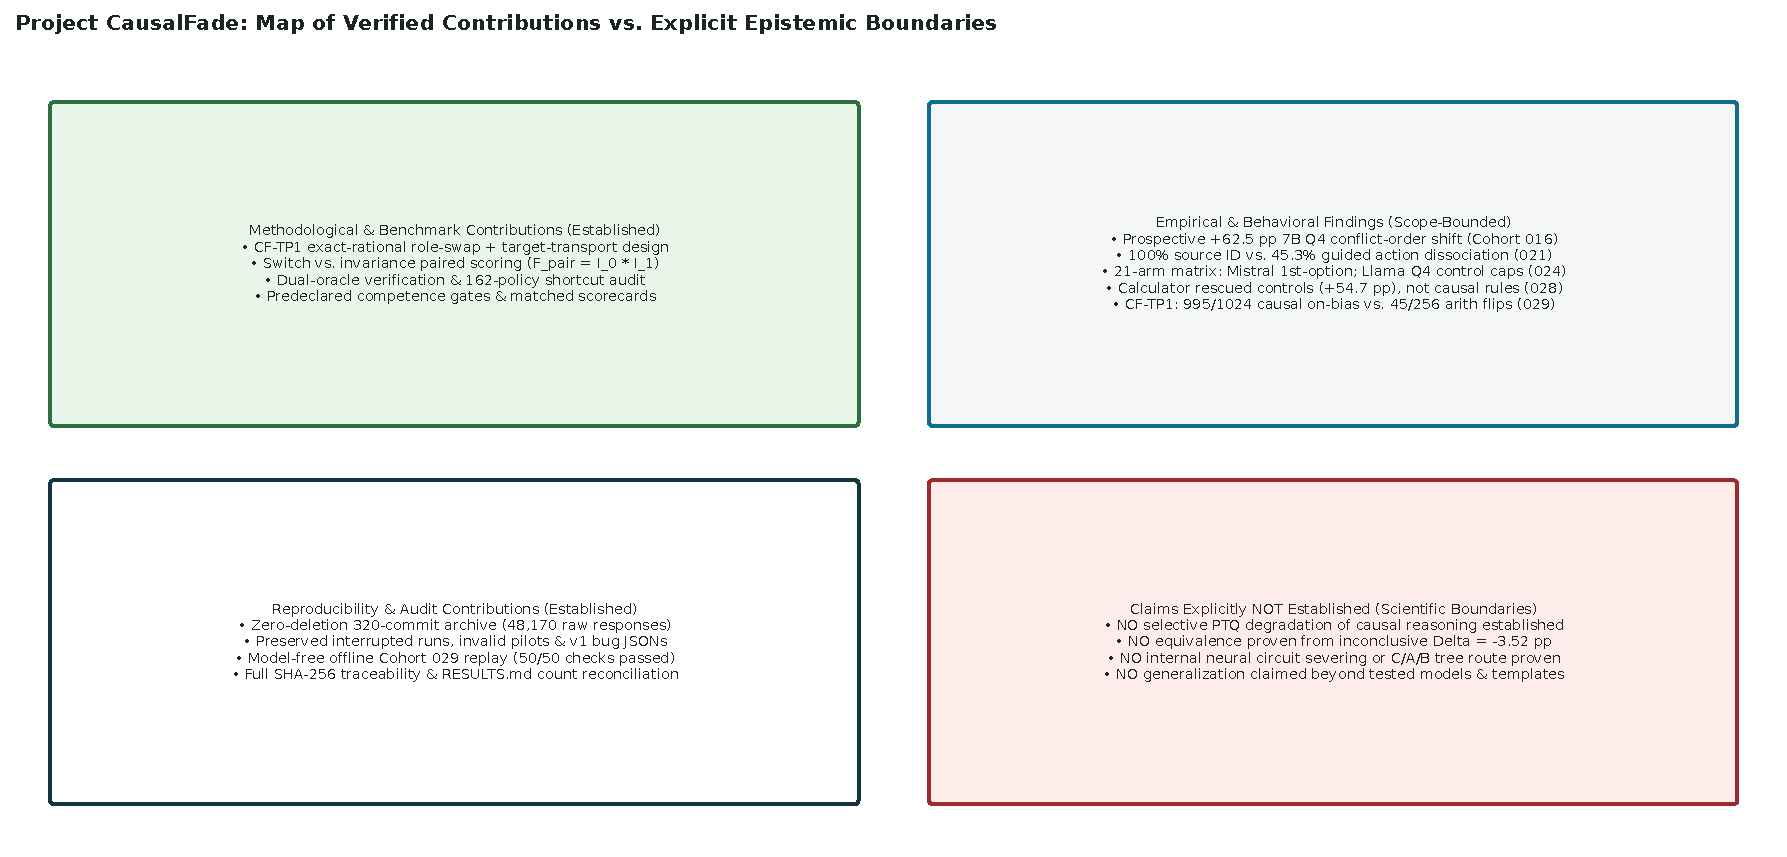
\includegraphics[width=\textwidth]{figures/fig17_research_contribution_map.pdf}
  \caption{Synthesis of CausalFade's lasting scientific contributions across benchmark design, psychometric/diagnostic methodology, LLM failure taxonomy, and reproducibility engineering.}
  \label{fig:contrib_map}
\end{figure}

\section{What CausalFade Established}
\begin{enumerate}
  \item \textbf{The \texttt{CF-TP1} Target-Transport Benchmark Architecture:} An exact-rational, role-symmetric, $162$-policy shortcut-audited benchmark uniting causal provenance selection with subgroup effect transportability and matched noncausal scorecard controls.
  \item \textbf{Pairwise Reversal-and-Retention Decomposition:} Practical demonstration that single-item binary accuracy ($\approx 50\%$) and even aggregate contrast-pair fidelity ($25.0\%$ vs.\ $28.5\%$) conceal radically different underlying policies unless partitioned into required reversals ($3/256$ vs.\ $27/256$) and required invariances ($125/256$ vs.\ $119/256$).
  \item \textbf{Empirical Proof of Three Fundamental Dissociations in Open-Weight Instruction LLMs ($3\text{B}$--$14\text{B}$):}
    \begin{itemize}
      \item \emph{Numeric computation vs.\ explicit action commitment} (Cohorts~002, 006, 007: $95.3\%$--$95.8\%$ ATE sign accuracy vs.\ $0\%$ activation);
      \item \emph{Declarative causal source recognition vs.\ two-source decision integration} (Cohorts~020--022: $100\%$ governing-source ID vs.\ $45.3\%$ guided decisions);
      \item \emph{Tool-assisted arithmetic execution vs.\ structural causal rule selection} (Cohort~028: $+54.69\pp$ Python calculator rescue on noncausal controls vs.\ $+2.34\pp$ on confounder/mediator selection).
    \end{itemize}
  \item \textbf{A Concrete Real-World Shortcut Counterexample (Cohort~016):} Demonstrating on an actual $1{,}536$-response experiment how a $p = 1.24\times 10^{-37}$ prospective replication can coexist with a $100\%$-accurate ($768/768$) source-blind numerical gap shortcut.
\end{enumerate}

\section{What CausalFade Explicitly Did \emph{Not} Establish}
\begin{enumerate}
  \item \textbf{No Selective Quantization Degradation of Causal Reasoning:} Across $48{,}170$ responses, compression never selectively eroded causal reasoning relative to a competent baseline; observed quantization differences reflected 3B arithmetic formula errors (\texttt{Q4\_K\_M}, Cohorts~002/007), 3B 2-bit token looping (\texttt{Q2\_K}, Cohort~001/003), template-specific 7B order sensitivity (Cohort~016), or 8B control-prompt verbosity truncation (\texttt{Llama Q4\_K\_M}, Cohort~024).
  \item \textbf{No Cross-Model or Chain-of-Thought Generalization of Cohort~029:} Cohort~029 evaluated a single open-weight quantized checkpoint (\texttt{Qwen2.5-7B-Instruct Q4\_K\_M}) under stateless single-JSON output without chain-of-thought reasoning tokens or external calculators; how frontier reasoning models or scratchpad-enabled agents perform on \texttt{CF-TP1} remains an open empirical question (Chapter~28).
\end{enumerate}


% --- PART VI: THE MAKING OF THE PAPER ---
\part{The Making of the Paper}
% =============================================================================
% Part VI: The Making of the Paper (Chapters 24--25)
% =============================================================================
\chapter{From Experimental Archive to Manuscript}\label{ch:making_paper}

When empirical data collection concluded on November 25, 2026 at tag \texttt{cohort-029-v1.0.0}, the researchers faced a formidable editorial challenge: how do you distill 30 experimental cohorts, 71 LLM run directories, $48{,}170$ raw completions, falsified psychometric trees, broken parsers, and twenty-eight developmental pivots into a concise, coherent journal submission without rewriting history or hiding negative results?

Inspecting the self-contained publication package in \texttt{manuscript/} (\texttt{article.tex}, \texttt{supplement.tex}, \texttt{history.tex}, \texttt{Scientific-and-editorial-QC.md}, \texttt{scripts/extract.py}, \texttt{scripts/figures.py}, and \texttt{audit/claim-ledger.csv}) reveals a remarkably principled three-tier editorial architecture:

\section{The Three-Document Publication Architecture}

\begin{enumerate}
  \item \textbf{The Main Research Article (\texttt{manuscript/article.tex}):} Framed cleanly as a \textbf{methodological benchmark and diagnostic case study} rather than a quantization paper. It centers on two verified pillars regenerated directly from raw bytes by \texttt{manuscript/scripts/extract.py}:
    \begin{itemize}
      \item \emph{The Diagnostic Motivation (Cohort~016 Counterexample, Figure~5 of \texttt{article.tex}):} Uses Cohort~016's $96$-family archive transparently as a concrete demonstration of how high apparent causal conflict accuracy ($91.1\%$ historical-first) and dramatic order swings ($+62.5\pp$) can arise inside a benchmark solvable $100\%$ of the time ($768/768$) by a source-blind smaller-gap heuristic.
      \item \emph{The Constructive Solution and Confirmatory Case Study (\texttt{CF-TP1}, Cohort~029, Figures~1--4 of \texttt{article.tex}):} Presents the exact-rational target-population transport protocol, worked Family~\texttt{096}, balanced $2\times 2$ sign-matrix design, $162$-policy shortcut audit, inconclusive primary contrast ($\widehat{\Delta} = -3.52\pp$, Welch $t$ CI $[-7.77, +0.74]\pp$; bounded CI $[-27.52, +20.49]\pp$), and the secondary pairwise reversal/invariance decomposition ($3/256$ causal switches vs.\ $27/256$ arithmetic switches and $45/256$ invariant flips).
    \end{itemize}
  \item \textbf{The Technical Supplement (\texttt{manuscript/supplement.tex}):} Supplies complete secondary tables (archive-form parity $128/512$ vs.\ $128/512$, role-pair and order-pair matrices, directional gold-off/gold-on counts $14/512$ and $497/512$, option-order breakdowns, and exhaustive $162$-policy shortcut audit bounds).
  \item \textbf{The Research History Disclosure (\texttt{manuscript/history.tex}):} Explicitly discloses that \texttt{CF-TP1} emerged from twenty-eight prior exploratory and developmental cohorts (\texttt{001}--\texttt{028}), summarizing the abandoned quantization hypothesis, reference-gate stops, and component/calculator ablations so no reader or referee could mistake Cohort~029 for a first-try one-shot experiment!
\end{enumerate}

\section{Editorial Selection vs.\ Full Archival Preservation}
What moved out of \texttt{article.tex} during manuscript distillation, and why?
\begin{itemize}
  \item \textbf{Excluded from main-text confirmatory claims:} Cohorts~001--015 and 017--028. Because those cohorts were exploratory development screens, reused families (001--003, 006, 008--009, 012, 017), failed pre-declared reference gates (004, 012, 014, 018, 019, 024, 026, 027, 028), or suffered post-hoc discovered confounds (Cohort~026 option-order coupling), elevating any of them alongside Cohort~029's frozen confirmatory protocol would have blurred exploratory and confirmatory inference.
  \item \textbf{Trade-off of editorial conciseness:} While \texttt{article.tex}'s tight focus on Cohort~029 + Cohort~016 maximizes statistical cleanliness for a journal audience (such as \emph{IEEE TNNLS}, evidenced by \texttt{manuscript/ieee-tnnls.log}), a reader of \texttt{article.tex} alone does not see the rich empirical gems of Cohort~007 ($-31.25\pp$ formula sign drop), Cohort~021 ($128/128$ source ID vs.\ $58/128$ guided action), Cohort~024 ($21$-arm SDT plane and Llama \texttt{Q4\_K\_M}'s $448$ control truncations), or Cohort~028 ($+54.69\pp$ Python calculator noncausal rescue vs.\ $+2.34\pp$ causal null). Preserving those twenty-eight cohorts in full depth is precisely why this retrospective monograph exists alongside the journal paper.
\end{itemize}

\section{Byte-Level Claim Auditing}
Perhaps the most admirable engineering practice in \texttt{manuscript/} is \texttt{manuscript/scripts/extract.py} (148 lines) paired with \texttt{manuscript/audit/claim-ledger.csv}. Rather than copying numbers from Markdown summaries (which would have propagated the manual \texttt{121/512, 416/512} typo in \texttt{experiments/cohort\_029/release/RESULTS.md}!), \texttt{extract.py} decodes all $4{,}096$ base64 HTTP payloads directly from \texttt{events.jsonl}, verifies every SHA-256 hash, re-parses every JSON completion with duplicate-key rejection, recomputes every pair count and Welch $t$ interval from scratch, asserts machine-precision agreement (\texttt{< 1e-12}) with \texttt{primary.json}, and writes the exact CSVs read by \texttt{figures.py} and verified against \texttt{article.tex}!

% =============================================================================
\chapter{The Original Hypothesis Revisited}\label{ch:revisited}

Let us return directly to October 28, 2026 (commit \texttt{4e2fe4f}) and place the founding hypothesis of Project CausalFade on the witness stand:

\begin{quote}
\textbf{Original Hypothesis (\texttt{H01}):} \emph{Post-training weight quantization selectively degrades interventional causal reasoning faster than surface associative processing, inflating $\mathrm{ConflictPenalty}(p) = \mathrm{Acc}_{\mathrm{aligned}}(p) - \mathrm{Acc}_{\mathrm{conflict}}(p)$ relative to unquantized \texttt{F16} models.}
\end{quote}

\section{Why \texttt{H01} Was Neither Confirmed Nor Trivially Falsified---It Was Exposed as Ill-Posed on Current 3B--8B Baselines}

If a student asks, \emph{``So was CausalFade's original hypothesis right or wrong?''}, the scientifically precise answer has three parts:

\begin{enumerate}
  \item \textbf{Empirically, selective quantization inflation of causal confounding vulnerability was NEVER established.} In Cohorts~005 and 011, 4-bit quantization (\texttt{Q4\_K\_M}) changed the conflict penalty by \textbf{$-43.75\pp$} and \textbf{$-39.06\pp$}---the \emph{opposite} direction of \texttt{H01}---because quantization pushed \texttt{Qwen2.5-3B} closer to a $100\%$ \texttt{activate=1} policy where aligned and conflict accuracy both equal $50\%$. In Cohort~015, \texttt{7B Q4\_K\_M} scored $+7.0\pp$ \emph{higher} overall than \texttt{F16}. In Cohort~024's $30{,}912$-request cross-lineage matrix, \texttt{Qwen 7B F16} vs.\ \texttt{Q4\_K\_M} differed by $-0.39\pp$ ($111/256$ vs.\ $110/256$) and \texttt{Llama 8B F16} vs.\ \texttt{Q4\_K\_M} differed by $+1.56\pp$ ($146/256$ vs.\ $150/256$) on semantic causal conflict, while \texttt{Llama Q4\_K\_M} collapsed by $-47.66\pp$ on \emph{noncausal controls} due to length-capped verbosity!
  \item \textbf{Where quantization DID hurt performance, the mechanism was noncausal.} \texttt{3B Q2\_K} failed via syntactic token-looping (\texttt{0/64}, Cohorts~001/003); \texttt{3B Q4\_K\_M} failed via explicit decimal formula arithmetic (\texttt{-25.0} to \texttt{-31.25} pp equally on aligned and conflict items, Cohorts~002/006/007); \texttt{7B Q4\_K\_M} amplified study-line recency sensitivity on one specific prompt template (\texttt{+44.79} pp interaction in Cohort~016, \texttt{0} pp in Cohort~024); and \texttt{Llama 8B Q4\_K\_M} lost JSON conciseness on scorecard controls (Cohort~024).
  \item \textbf{More fundamentally, testing whether compression ``erodes'' causal reasoning presupposes that the uncompressed model possesses causal reasoning to lose!} Across Cohorts~004, 012, 018--024, 027, and 028, unquantized \textbf{\texttt{F16}} models ($3\text{B}$--$8\text{B}$) failed single-pass backdoor standardization, failed two-source conflict integration ($43\%$--$57\%$), failed harmful-direction controls, obeyed first-option policies (\texttt{Mistral F16}: $256/256$), scored $0/8$ on order-balanced confounder-vs.-mediator switches, and selected causal adjustment procedures at chance ($53.1\%$ and $46.9\%$) even with a Python calculator! You cannot measure the ``fading'' of a capability whose baseline signal is zero ($0.031\;\text{bits}$ mutual information in Cohort~025).
\end{enumerate}

\section{Why Discovering This Truth Surpassed the Original Goal}
Had CausalFade stopped after Cohort~015 or Cohort~016, or had it lacked matched noncausal controls and option-order counterbalancing, it could easily have published a misleading claim about quantized causal fragility. By following the evidence ruthlessly wherever it led---even when it meant dismantling the project's own namesake premise---CausalFade uncovered a far more general truth about how language models process quantitative evidence and how causal benchmarks must be built.


% --- PART VII: WHAT CAUSALFADE TEACHES US ---
\part{What CausalFade Teaches Us}
% =============================================================================
% Part VII: What CausalFade Teaches Us (Chapters 26--29)
% =============================================================================
\chapter{Lessons in Scientific Research}\label{ch:lessons_research}

For students and fellow researchers embarking on empirical AI investigations, Project CausalFade offers eight concrete methodological lessons---none of them abstract platitudes, each paid for in real debugging hours across the repository's 320 commits:

\begin{enumerate}
  \item \textbf{Validate Your Estimators on Synthetic Truth Before Querying Real Models (\texttt{design\_validation}).} Running $3{,}600$ synthetic EM fits \emph{before} Cohort~001 cost minutes of CPU time and immediately revealed that the 3-parameter $C/A/B$ tree was observationally equivalent to symmetric logistic integration ($p=0.433$) and unstable near $C \to 1$. Pre-experiment simulation tells you what your statistical microscope can and cannot resolve.
  \item \textbf{Audit Raw Completions Before Trusting Aggregate Scores (Cohorts~001, 013, 024, 026).} In Cohort~001, \texttt{0/64} strict accuracy hid valid JSON inside Markdown fences. In Cohort~013, \texttt{0/64} hid valid JSON followed by trailing causal essays. In Cohort~024, \texttt{Llama Q4\_K\_M}'s control drop (\texttt{78/256}) was $448$ truncated prose explanations rather than wrong JSON choices. In Cohort~026, \texttt{Llama v2}'s \texttt{48/112} validity was a single trailing period (\texttt{"X=1."}). \textbf{Always inspect raw responses and separate format validity from semantic accuracy.}
  \item \textbf{Single-Item Binary Accuracy Is Blind to Constant Priors and Positional Policies (Cohorts~005, 024, 029).} Any binary benchmark with balanced labels grants $50\%$ accuracy and $0\pp$ conflict penalty to a constant \texttt{activate=1} policy (\texttt{995/1,024} in Cohort~029) or a \texttt{pick-first-option} policy (\texttt{256/256} in Cohort~024 \texttt{Mistral F16}). Always report directional class accuracies (\texttt{Gold=0} vs.\ \texttt{Gold=1}), counterbalanced option-flip consistency, and pairwise bundle fidelity ($F_{\mathrm{pair}} = I_0 I_1$).
  \item \textbf{Be Most Skeptical of Your Most Spectacular $p$-Value (Cohort~016).} Cohort~016 achieved $t(95)=21.10$, $p = 1.24\times 10^{-37}$ on a pre-registered 96-family replication---the dream statistic of many empirical papers. Yet cross-scale testing in Cohort~017 (\texttt{14B}: $0\pp$), cross-scaffold testing in Cohort~024 ($0\pp$), and retrospective magnitude auditing ($768/768$ solvable by picking the smaller printed gap) showed how fragile and shortcut-ridden that benchmark actually was. \textbf{Tiny $p$-values measure random sampling noise across worlds, NOT construct validity.}
  \item \textbf{Never Attribute Failure to a High-Level Construct Without a Matched Low-Level Control (Cohorts~002, 023, 028, 029).} Whenever an LLM fails a ``causal reasoning'' prompt, ask first whether it passes the exact same numerical operation stripped of causal framing. Cohort~023 (\texttt{58.6\%} harmful-direction control), Cohort~028 (\texttt{45.3\%} mental named-rule math vs.\ \texttt{100\%} with calculator), and Cohort~029 (\texttt{28.52\%} arithmetic pair fidelity) proved that baseline multi-number aggregation is a massive confound in single-pass LLM evaluation.
  \item \textbf{Pre-Declare Reference Competence Gates---and Obey Them When They Fail (Cohorts~004, 012, 018, 019, 026--028).} Stopping an experiment when the unquantized baseline fails (\texttt{stopped\_by\_gate}) feels painful in the moment, but it prevents polluting literature with meaningless comparisons between two broken systems.
  \item \textbf{Never Delete Failed Pilots, Interrupted Logs, or Buggy Analyzer Versions (Cohorts~008, 009--011, 017, 026).} Preserving \texttt{cohort\_008/run\_001\_f16} (\texttt{26/64}), \texttt{source\_order\_analysis\_v1\_undercounted\_counts.json}, Cohort~017's missing-NumPy trace, and \texttt{cohort\_026/invalidated\_pilot\_qwen\_v1} (\texttt{112} calls) with explicit README explanations created an unassailable audit trail.
  \item \textbf{Automate End-to-End Number Extraction From Raw Cryptographic Logs (\texttt{manuscript/scripts/extract.py}).} The \emph{only} numerical discrepancy found in the entire Cohort~029 release (\texttt{121/512, 416/512} vs.\ \texttt{14/512, 497/512} in \texttt{RESULTS.md}) occurred where prose was typed manually rather than generated from \texttt{events.jsonl}. Machine-verified extraction pipelines eliminate human transcription error.
\end{enumerate}

% =============================================================================
\chapter{Lessons in Causal AI}\label{ch:lessons_causal_ai}

Beyond general research methodology, CausalFade yields four sharp substantive insights into how current open-weight instruction-tuned transformers ($3\text{B}$--$14\text{B}$ parameters) interact with causal inference problems:

\section{1. Declarative Causal Knowledge $\neq$ Procedural Causal Execution}
Across multiple cohorts, models demonstrated near-perfect \emph{declarative} familiarity with textbook causal rules when queried in isolation: \texttt{Qwen2.5-7B F16} named the valid backdoor adjustment set \texttt{["Z"]} on $32/32$ ($100\%$) of Cohort~004 prompts and identified the randomized study as the governing causal source on $128/128$ ($100\%$) of Cohort~021--022 prompts, while \texttt{Llama-3.1-8B F16} answered direct causal graph ancestry questions at $31/32$ ($96.9\%$) in Cohort~027. Yet those exact same models failed completely to \emph{bind} that declarative rule to numerical selection and weighting in a single forward pass ($17/32$ actions in Cohort~004; $58/128$ guided actions in Cohort~021; $0/8$ graph switches in Cohort~027). Current instruction-tuned LLMs store verbal rules about causality without reliably compiling them into single-pass computational routing over tabular numbers.

\section{2. Tool Calculators Solve Estimation Arithmetic---Not Causal Identification}
A popular assumption in agentic AI is that coupling an LLM to a Python interpreter or calculator solves quantitative causal inference. Cohort~028 tested that assumption directly in a zero-leakage controlled ablation: an allowlisted deterministic Python calculator (\texttt{System C}) vaulted \texttt{Qwen2.5-7B F16} from $45.3\%$ to \textbf{$100.0\%$ ($128/128$)} on matched noncausal tasks where the rule name (\texttt{marginal} vs.\ \texttt{conditional}) was stated explicitly, yet yielded \textbf{$53.1\%$ ($68/128$, $+2.34\pp$)} on causal confounder-vs.-mediator tasks (\texttt{46.9\%} in \texttt{Llama-3.1-8B F16})! Externalizing calculation rescues \emph{statistical estimation} only if the agent can first solve \emph{structural causal identification}---mapping temporal/graphical structure onto the right adjustment functional \citep{pearl2009causality,sawarni2026crb,leban2026causalds}.

\section{3. Causal Framing Can Trigger Stronger Action Bias Than Neutral Framing}
One of Cohort~029's most surprising empirical discoveries was that \texttt{Qwen2.5-7B Q4\_K\_M} behaved \emph{more} degenerately under natural-prose causal advising (\texttt{995/1,024 = 97.17\%} \texttt{activate=1}; \texttt{3/256} target switches; \texttt{3/256} source-role switches) than under matched noncausal scorecard wording on the exact same numbers (\texttt{597/1,024 = 58.30\%} \texttt{activate=1}; \texttt{27/256} target switches; \texttt{67/256} source-role switches)! Why? Advisory prompts asking \emph{``whether switching a certain setting on would raise the success rate''} appear to activate strong RLHF/instruction-tuning helpfulness or affirmative-intervention priors (\texttt{activate=1}) whenever multi-table uncertainty exceeds single-pass capacity.

\section{4. Transportability and Pairwise Counterfactual Perturbations Are the Right Testbed}
Static observational question answering conflates memorized domain priors with causal reasoning, while two-study aggregate comparisons collapse into trivial single-pair inequalities once a study is chosen. Target-population transportability under subgroup heterogeneity (\texttt{CF-TP1})---requiring an agent to reverse its recommendation when target composition crosses $w_{\mathrm{crit}}$~\eqref{eq:w_crit} and retain its recommendation when it does not---provides an algebraic, domain-neutral litmus test for genuine interventional competence.

% =============================================================================
\chapter{The Unanswered Questions}\label{ch:unanswered}

Because Project CausalFade prioritized methodological rigor over overclaiming, its conclusion opens four crisp, directly testable research programs. For each open question, we specify the exact experimental design and controls required so future investigators do not repeat the pitfalls uncovered in Cohorts~001--028.

\section{1. Does Chain-of-Thought or Scratchpad Generation Unlock \texttt{CF-TP1} and Graph Switching?}
\begin{itemize}
  \item \textbf{The Open Question:} Cohort~029 (\texttt{CF-TP1}) and Cohorts~027--028 constrained models to emit bare tokens (\texttt{X=1}) or single-key JSON (\texttt{\{"activate":1\}}) in a single stateless pass without intermediate reasoning tokens. Since computing $w^* \mu_{\mathrm{rct}}(0,a) + (1-w^*)\mu_{\mathrm{rct}}(1,a)$ requires multi-step arithmetic and source filtering, how much of Cohort~029's failure disappears when explicit chain-of-thought scratchpads or reasoning-tuned test-time compute are permitted?
  \item \textbf{Proposed Controlled Design:} Evaluate \texttt{CF-TP1}'s exact frozen $4{,}096$-prompt fixture under a crossed $2\times 2$ generation regime: \emph{(no-scratchpad single JSON vs.\ structured scratchpad + final JSON)} $\times$ \emph{(causal transport vs.\ matched arithmetic scorecard)}, with generous \texttt{max\_tokens} ($\ge 1{,}024$) to prevent \texttt{Lian et al.} token-inflation truncation.
  \item \textbf{Diagnostic Criterion:} If scratchpad reasoning raises \emph{both} arithmetic and causal target-pair fidelity to $>85\%$, Cohort~029's collapse was a single-pass working-memory bottleneck; if scratchpads raise arithmetic to $>90\%$ while causal remains stalled (mirroring Cohort~028's calculator split!), the bottleneck is genuinely causal provenance/transport identification.
\end{itemize}

\section{2. Does \texttt{H01} (Selective Quantization Decay) Emerge Once Reference Models Pass \texttt{CF-TP1}?}
\begin{itemize}
  \item \textbf{The Open Question:} CausalFade could never test selective quantization decay of genuine causal transport because \texttt{3B}--\texttt{8B} single-pass models sat at the $25\%$ floor even at \texttt{F16}. What happens when a model/scaffold combination \emph{actually clears} $\ge 80\%$ switch-pair and invariant-pair fidelity at \texttt{F16}/\texttt{BF16} (e.g., \texttt{32B}--\texttt{70B} models or scratchpad-enabled \texttt{7B}--\texttt{14B} reasoning models) and is then compressed across \texttt{Q8\_0}, \texttt{Q6\_K}, \texttt{Q4\_K\_M}, \texttt{Q3\_K\_M}, and \texttt{Q2\_K} (both with and without \texttt{imatrix} calibration and QAT)?
  \item \textbf{Proposed Controlled Design:} Pre-register a reference gate requiring $\ge 80\%$ switch-pair fidelity and $\ge 80\%$ invariant-pair fidelity on \emph{both} causal and arithmetic \texttt{CF-TP1} splits at \texttt{BF16}/\texttt{F16}, then estimate the double difference $\Delta_{\mathrm{PTQ}}(p) = [F_{\mathrm{causal}}(p) - F_{\mathrm{causal}}(\text{F16})] - [F_{\mathrm{arith}}(p) - F_{\mathrm{arith}}(\text{F16})]$ across family clusters.
\end{itemize}

\section{3. Why Do Models Fail Confounder-vs.-Mediator Rule Selection With a Calculator (Cohort~028)?}
\begin{itemize}
  \item \textbf{The Open Question:} In Cohort~028, \texttt{Qwen 7B F16} and \texttt{Llama 8B F16} achieved $97\%$--$100\%$ direct graph-ancestry reading yet chose \texttt{marginal} vs.\ \texttt{conditional} weighting at $\sim 50\%$ chance even when both candidate definitions were written in the prompt. Is the failure caused by unfamiliar terminology (\texttt{marginal} vs.\ \texttt{conditional}), inability to trace backdoor vs.\ frontdoor/mediator causal logic, or confusion when both $P(W)$ and $P(W\mid X)$ appear simultaneously in the prompt?
  \item \textbf{Proposed Controlled Design:} Extend Cohort~028's \texttt{System C} calculator pipeline with a multi-stage Socratic decomposition: Stage~1 asks \emph{``Does X cause W, or does W cause X?''}; Stage~2 asks \emph{``If we intervene to set X=x, does the distribution of W stay at P(W) or change to P(W|X=x)?''}; Stage~3 dispatches the chosen distribution to the deterministic calculator.
\end{itemize}

\section{4. Mechanistic Localization Once Behavioral Competence Is Verified}
\begin{itemize}
  \item \textbf{The Open Question:} CausalFade rightly foreswore ``circuit severing'' claims (\texttt{D01}) because behavioral competence was absent. On a model that \emph{passes} \texttt{CF-TP1} ($>85\%$ switch and invariant fidelity), how do attention heads bind provenance tags (\texttt{randomized study}) to downstream stratum tables while suppressing confounded distractor tables?
  \item \textbf{Proposed Controlled Design:} Perform causal mediation / activation patching across \texttt{CF-TP1}'s minimal role-swap pairs (prompts differing \emph{only} by swapping the words \texttt{randomized} and \texttt{historical} between Source~A and Source~B on identical numerical tables), localizing the exact layers where provenance flips reverse the output logit difference.
\end{itemize}

% =============================================================================
\chapter{Epilogue}\label{ch:epilogue}

Twenty-nine days is a brief span on a calendar, yet in the life of a rigorously conducted research project it can encompass an entire scientific education. Project CausalFade set out on October 28, 2026 hoping to measure how weight compression erodes causal reasoning in local language models. Along the way, it encountered nearly every trap waiting for modern AI evaluators: Markdown fences masquerading as model incompetence, 2-bit token loops, psychometric models that looked principled on paper yet violated additivity on real outputs, numeric estimates that disagreed with a model's own actions on the very same line, a $p = 1.24 \times 10^{-37}$ prospective confirmation undermined by an unnoticed numerical gap invariant, $100\%$ first-option positional policies, and 4-bit verbosity truncations that struck control prompts while sparing causal ones.

What makes CausalFade worthy of study is not that those traps appeared---they appear silently in dozens of published LLM benchmarks every month---but that \textbf{every time the evidence contradicted an appealing narrative, the researchers listened to the evidence}. They did not delete failed cohorts. They did not hide interrupted runs or post-run script bugs. They did not promote an ungeneralizable $7\text{B}$ order swing as a universal law of compression, nor did they cherry-pick a confounded $6/8$ graph-switch run when counterbalancing dropped it to $0/8$. And when their culminating $4{,}096$-prompt confirmatory study (\texttt{CF-TP1}) yielded an inconclusive $-3.52\pp$ difference between causal transport and matched weighted arithmetic, they reported the null plainly---while showing through pairwise reversal and retention analysis exactly \emph{how} a language model can score $50\%$ on items while failing $98.8\%$ of required causal reversals.

Science advances at least as much by sharpening our instruments and exposing false positives as by announcing triumphs. In trading an unidentifiable story about quantization fade for a permanent, shortcut-audited diagnostic methodology, Project CausalFade fulfilled the highest obligation of empirical inquiry: leaving the field clearer, harder to fool, and better equipped to tell genuine causal reasoning apart from its many imitations.


% =============================================================================
% APPENDICES & BIBLIOGRAPHY
% =============================================================================
\appendix
\part*{Appendices}
\addcontentsline{toc}{part}{Appendices}
% =============================================================================
% Appendices A through I
% =============================================================================

\chapter{Master Cohort Inventory}\label{app:cohort_inventory}
Table~\ref{tab:cohort_master} catalogs all thirty-one methodological and empirical cohort units in Project CausalFade (\texttt{design\_validation} and Cohorts~\texttt{001}--\texttt{029}, including \texttt{025\_1}), extracted programmatically from \texttt{evidence/cohort\_inventory.csv}.

{\footnotesize
\setlength{\tabcolsep}{3.5pt}
\begin{longtable}{@{}>{\raggedright\arraybackslash}p{1.8cm}>{\raggedright\arraybackslash}p{1.6cm}>{\raggedright\arraybackslash}p{2.6cm}>{\raggedright\arraybackslash}p{1.1cm}>{\raggedright\arraybackslash}p{3.4cm}>{\raggedright\arraybackslash}p{4.3cm}@{}}
\caption{Master inventory of all 31 CausalFade methodological and empirical cohort units (\texttt{design\_validation} and Cohorts \texttt{001}--\texttt{029}, including \texttt{025\_1}).}\label{tab:cohort_master}\\
\toprule
\textbf{Cohort} & \textbf{Dates} & \textbf{Models / Arms} & \textbf{Pers.} & \textbf{Design \& Classification} & \textbf{Principal Empirical Finding} \\
\midrule
\endfirsthead
\toprule
\textbf{Cohort} & \textbf{Dates} & \textbf{Models / Arms} & \textbf{Pers.} & \textbf{Design \& Classification} & \textbf{Principal Empirical Finding} \\
\midrule
\endhead
\bottomrule
\endfoot
\texttt{design\_validation} & 2026-\allowbreak{}11-\allowbreak{}01 & None (3,600 synthetic datasets) & 0 & 24 families (192 prompts) + 3,600 EM fits (Exploratory synthetic validation) & Recovered C/\allowbreak{}A/\allowbreak{}B away from boundaries; exposed symmetric logistic observational equivalence and 16 near-\allowbreak{}boundary nonconvergences \\[2pt]
\texttt{cohort\_001} & 2026-\allowbreak{}11-\allowbreak{}10 & Qwen2.5-\allowbreak{}3B (F16, Q2\_K, Q4\_K\_M) & 192 & 16 dev families, 64 exact prompts/\allowbreak{}arm (Exploratory pilot) & Strict 0/\allowbreak{}64 all arms (Markdown fences); fence-\allowbreak{}only F16 33/\allowbreak{}64 (63/\allowbreak{}64 activate, 0/\allowbreak{}64 adj set), Q2\_K 0/\allowbreak{}64 (64/\allowbreak{}64 length-\allowbreak{}capped), Q4\_K\_M 34/\allowbreak{}64 \\[2pt]
\texttt{cohort\_002} & 2026-\allowbreak{}11-\allowbreak{}10 & Qwen2.5-\allowbreak{}3B (F16, Q4\_K\_M) & 128 & Same 16 families, 64 formula prompts/\allowbreak{}arm (Exploratory control) & Fence-\allowbreak{}only explicit action: F16 32/\allowbreak{}64 (0/\allowbreak{}64 activate), Q4 35/\allowbreak{}64 (3/\allowbreak{}64 activate); estimate signs: F16 61/\allowbreak{}64 vs Q4 45/\allowbreak{}64 (-\allowbreak{}25.0 pp) \\[2pt]
\texttt{cohort\_003} & 2026-\allowbreak{}11-\allowbreak{}10 & Qwen2.5-\allowbreak{}3B Q2\_K (default vs -\allowbreak{}-\allowbreak{}no-\allowbreak{}repack) & 32 & 4 dev families, 16 exact prompts/\allowbreak{}arm (Technical diagnostic) & 0/\allowbreak{}16 valid and 16/\allowbreak{}16 length-\allowbreak{}capped in both arms; disabling repacking altered token strings on 16/\allowbreak{}16 items without rescuing output \\[2pt]
\texttt{cohort\_004} & 2026-\allowbreak{}11-\allowbreak{}10 & Qwen2.5-\allowbreak{}7B F16 & 32 & 8 dev families, 32 exact prompts (Exploratory feasibility gate) & Fence-\allowbreak{}only 17/\allowbreak{}32 overall (failed >=22/\allowbreak{}32 gate), 9/\allowbreak{}16 conflict, 31/\allowbreak{}32 activate, 32/\allowbreak{}32 adjustment set [Z] correct; 7B Q2\_K withheld \\[2pt]
\texttt{cohort\_005} & 2026-\allowbreak{}11-\allowbreak{}10 & Qwen2.5-\allowbreak{}3B (F16, Q4\_K\_M) & 128 & 16 dev families, 64 supplied-\allowbreak{}rate prompts/\allowbreak{}arm (Exploratory diagnostic) & Fence-\allowbreak{}only F16 39/\allowbreak{}64 (28/\allowbreak{}32 aligned, 11/\allowbreak{}32 conflict), Q4 35/\allowbreak{}64 (19/\allowbreak{}32 aligned, 16/\allowbreak{}32 conflict, 61/\allowbreak{}64 activate); F16 C/\allowbreak{}A/\allowbreak{}B additivity residual -\allowbreak{}43.75 pp \\[2pt]
\texttt{cohort\_006} & 2026-\allowbreak{}11-\allowbreak{}10 & Qwen2.5-\allowbreak{}3B Q8\_0 (vs archived F16, Q4\_K\_M) & 64 & 16 reused families, 64 formula prompts (Exploratory control follow-\allowbreak{}up) & Fence-\allowbreak{}only Q8\_0 estimate sign 61/\allowbreak{}64 (tied F16, +25.0 pp over Q4), explicit action 32/\allowbreak{}64 (0/\allowbreak{}64 activate) \\[2pt]
\texttt{cohort\_007} & 2026-\allowbreak{}11-\allowbreak{}10 & Qwen2.5-\allowbreak{}3B (F16, Q4\_K\_M) & 96 & 12 fresh families (seed 20261111), 48 prompts/\allowbreak{}arm (Exploratory fresh-\allowbreak{}family replication) & Estimate sign replicated: F16 46/\allowbreak{}48 vs Q4 31/\allowbreak{}48 (-\allowbreak{}31.25 pp, 95\% CI [-\allowbreak{}41.67, -\allowbreak{}20.83]); explicit actions 24/\allowbreak{}48 vs 28/\allowbreak{}48 \\[2pt]
\texttt{cohort\_008} & 2026-\allowbreak{}11-\allowbreak{}10 to 2026-\allowbreak{}11-\allowbreak{}12 & Qwen2.5-\allowbreak{}3B (F16 partial + F16, Q4\_K\_M complete) & 154 (192 sched) & 16 families, 64 reversed prompts/\allowbreak{}arm (+ 26/\allowbreak{}64 interrupted) (Exploratory crossover) & Run 1 interrupted at 25/\allowbreak{}64 (+1 error) for PC shutdown; rerun complete: F16 conflict 16/\allowbreak{}32 rand-\allowbreak{}first vs 7/\allowbreak{}32 hist-\allowbreak{}first (-\allowbreak{}28.125 pp); Q4 16/\allowbreak{}32 both \\[2pt]
\texttt{cohort\_009} & 2026-\allowbreak{}11-\allowbreak{}12 & Qwen2.5-\allowbreak{}3B (F16, Q4\_K\_M) & 256 & 16 reused families, 128 interleaved twin prompts/\allowbreak{}arm (Exploratory crossover) & Removed session confound: F16 conflict 16/\allowbreak{}32 rand-\allowbreak{}first vs 9/\allowbreak{}32 hist-\allowbreak{}first (-\allowbreak{}21.875 pp); Q4 16/\allowbreak{}32 both; count bug later fixed in b90cb63 \\[2pt]
\texttt{cohort\_010} & 2026-\allowbreak{}11-\allowbreak{}12 & Qwen2.5-\allowbreak{}3B (F16, Q4\_K\_M) & 192 & 12 fresh families (seed 20261113), 96 twin prompts/\allowbreak{}arm (Exploratory fresh-\allowbreak{}family replication) & F16 conflict 12/\allowbreak{}24 rand-\allowbreak{}first vs 6/\allowbreak{}24 hist-\allowbreak{}first (-\allowbreak{}25.0 pp, CI [-\allowbreak{}37.5, -\allowbreak{}12.5]); Q4 12/\allowbreak{}24 both; count bug fixed in b90cb63 \\[2pt]
\texttt{cohort\_011} & 2026-\allowbreak{}11-\allowbreak{}12 & Qwen2.5-\allowbreak{}3B (F16, Q4\_K\_M) & 256 & 16 fresh matched-\allowbreak{}strength families (seed 20261114), 128 prompts/\allowbreak{}arm (Exploratory development) & Repaired aligned vs conflict historical gap imbalance; F16 conflict 16/\allowbreak{}32 vs 8/\allowbreak{}32 (-\allowbreak{}25.0 pp), aligned 18/\allowbreak{}32 vs 32/\allowbreak{}32 (+43.75 pp); Q4 near-\allowbreak{}constant activate \\[2pt]
\texttt{cohort\_012} & 2026-\allowbreak{}11-\allowbreak{}12 & Qwen2.5-\allowbreak{}7B F16 & 64 & 8 reused cohort-\allowbreak{}011 families, 64 prompts (Exploratory feasibility gate) & Fence-\allowbreak{}only 47/\allowbreak{}64 overall, 32/\allowbreak{}32 aligned, but conflict 8/\allowbreak{}16 rand-\allowbreak{}first and 7/\allowbreak{}16 hist-\allowbreak{}first (failed >=9/\allowbreak{}16 per-\allowbreak{}order gate); Q4 withheld \\[2pt]
\texttt{cohort\_013} & 2026-\allowbreak{}11-\allowbreak{}12 & Qwen2.5-\allowbreak{}7B F16 & 128 & 8 fresh matched families (seed 20261116), 128 prompts (Exploratory crossover) & Minimal 48/\allowbreak{}64 fence-\allowbreak{}valid (8/\allowbreak{}16 conflict); causal-\allowbreak{}context 0/\allowbreak{}64 valid (all 64 appended prose after JSON and hit 160-\allowbreak{}token cap; prefix diag 45/\allowbreak{}64) \\[2pt]
\texttt{cohort\_014} & 2026-\allowbreak{}11-\allowbreak{}12 & Qwen2.5-\allowbreak{}7B F16 & 128 & 8 fresh matched families (seed 20261119), 128 prompts (Exploratory feasibility gate) & 128/\allowbreak{}128 strict-\allowbreak{}valid JSON! Minimal 48/\allowbreak{}64 (failed conflict 8/\allowbreak{}16, 8/\allowbreak{}16); Causal-\allowbreak{}context 42/\allowbreak{}64 (passed conflict 9/\allowbreak{}16, 9/\allowbreak{}16, missed overall >=44 by 2) \\[2pt]
\texttt{cohort\_015} & 2026-\allowbreak{}11-\allowbreak{}12 & Qwen2.5-\allowbreak{}7B (F16, Q4\_K\_M) & 256 & 16 fresh matched families (seed 20261122), 128 prompts/\allowbreak{}arm (Development gate + conditional comparison) & F16 passed gate (89/\allowbreak{}128 overall, 19/\allowbreak{}32 \& 22/\allowbreak{}32 conflict), triggering Q4 (98/\allowbreak{}128 overall); discovered Q4 conflict order jump: 11/\allowbreak{}32 rand-\allowbreak{}first vs 32/\allowbreak{}32 hist-\allowbreak{}first (+65.6 pp) \\[2pt]
\texttt{cohort\_016} & 2026-\allowbreak{}11-\allowbreak{}12 & Qwen2.5-\allowbreak{}7B (F16, Q4\_K\_M) & 1536 & 96 fresh matched families (seed 20261127), 768 prompts/\allowbreak{}arm (Prospective confirmatory replication) & Confirmed Q4 conflict order effect: 175/\allowbreak{}192 hist-\allowbreak{}first vs 55/\allowbreak{}192 rand-\allowbreak{}first (+62.5 pp, t(95)=21.10, p=1.24e-\allowbreak{}37); later retrospective audit found smaller-\allowbreak{}gap heuristic solves 768/\allowbreak{}768 \\[2pt]
\texttt{cohort\_017} & 2026-\allowbreak{}11-\allowbreak{}13 & Qwen2.5-\allowbreak{}14B (Q8\_0, Q4\_K\_M) & 1536 & 96 reused cohort-\allowbreak{}016 families, 768 prompts/\allowbreak{}arm (Exploratory cross-\allowbreak{}size extension) & Q8\_0 488/\allowbreak{}768 (conflict -\allowbreak{}4.17 pp), Q4\_K\_M 440/\allowbreak{}768 (conflict 0 pp, 100\% activate); 7B order effect did not generalize; missing-\allowbreak{}NumPy crash repaired locally \\[2pt]
\texttt{cohort\_018} & 2026-\allowbreak{}11-\allowbreak{}13 to 2026-\allowbreak{}11-\allowbreak{}14 & Qwen2.5-\allowbreak{}7B F16 & 288 & 8 fresh families (seed 20261114), 288 prompts (Development gate) & 288/\allowbreak{}288 strict-\allowbreak{}valid; failed gate (64/\allowbreak{}128 causal vs 80, 14/\allowbreak{}32 hist-\allowbreak{}first conflict vs 18); noncausal control 62/\allowbreak{}128; reversed token mapping collapsed accuracy (14/\allowbreak{}64 vs 50/\allowbreak{}64); Q4 withheld \\[2pt]
\texttt{cohort\_019} & 2026-\allowbreak{}11-\allowbreak{}14 & Qwen2.5-\allowbreak{}7B F16 & 832 & 8 fresh families (seed 20261115), 832 prompts (Development gate) & 832/\allowbreak{}832 strict-\allowbreak{}valid; semantic gate failed (73/\allowbreak{}128 causal, 12/\allowbreak{}32 \& 13/\allowbreak{}32 conflict, 24/\allowbreak{}32 comp); neutral reverse beat forward by +25.8 pp causal \& +36.7 pp control; source-\allowbreak{}check cue bug documented \\[2pt]
\texttt{cohort\_020} & 2026-\allowbreak{}11-\allowbreak{}14 & Qwen2.5-\allowbreak{}7B F16 & 224 & 8 fresh families (seed 20261116), 224 prompts (Component diagnostic) & 224/\allowbreak{}224 strict-\allowbreak{}valid; isolated components strong (number 28/\allowbreak{}32, rand-\allowbreak{}only 29/\allowbreak{}32, source ID 32/\allowbreak{}32), but two-\allowbreak{}source historical-\allowbreak{}first conflict dropped to 16/\allowbreak{}32 (0/\allowbreak{}32 activate) \\[2pt]
\texttt{cohort\_021} & 2026-\allowbreak{}11-\allowbreak{}14 & Qwen2.5-\allowbreak{}7B F16 & 576 & 8 fresh families (seed 20261117), 576 prompts (Guidance diagnostic) & 576/\allowbreak{}576 strict-\allowbreak{}valid; governing-\allowbreak{}source selection 128/\allowbreak{}128 (100\%) and rand-\allowbreak{}only 30/\allowbreak{}32, yet ordinary and source-\allowbreak{}guided two-\allowbreak{}source decisions both 58/\allowbreak{}128 (11 gains, 11 losses) \\[2pt]
\texttt{cohort\_022} & 2026-\allowbreak{}11-\allowbreak{}16 & Qwen2.5-\allowbreak{}7B F16, Mistral-\allowbreak{}7B-\allowbreak{}v0.3 Q4\_K\_M & 1152 & 8 fresh families (seed 20261118), 576 prompts/\allowbreak{}arm (Development cross-\allowbreak{}lineage screen) & Qwen repeated +53.1 pp rand-\allowbreak{}only vs two-\allowbreak{}source gap (source sel 128/\allowbreak{}128, rand-\allowbreak{}only 31/\allowbreak{}32, two-\allowbreak{}source 56/\allowbreak{}128); Mistral failed components (source sel 64/\allowbreak{}128 always 'A', rand-\allowbreak{}only 16/\allowbreak{}32 always activate) \\[2pt]
\texttt{cohort\_023} & 2026-\allowbreak{}11-\allowbreak{}16 & Qwen2.5-\allowbreak{}7B F16 & 896 & 8 fresh families (seed 20261119), 896 prompts (Measurement audit) & 896/\allowbreak{}896 strict-\allowbreak{}valid; simple components passed (rand-\allowbreak{}only 64/\allowbreak{}64, source sel 244/\allowbreak{}256) and +55.5 pp gap persisted across A/\allowbreak{}B \& option order, but harmful numeric (18/\allowbreak{}32) \& noncausal (75/\allowbreak{}128) failed >=75\% rule \\[2pt]
\texttt{cohort\_024} & 2026-\allowbreak{}11-\allowbreak{}16 to 2026-\allowbreak{}11-\allowbreak{}18 & Qwen2.5-\allowbreak{}7B, Mistral-\allowbreak{}7B-\allowbreak{}v0.3, Llama-\allowbreak{}3.1-\allowbreak{}8B x (F16, Q8\_0, Q6\_K, Q5\_K\_M, Q4\_K\_M, Q3\_K\_M, Q2\_K) & 30912 & 8 fresh families, 1,472 prompts x 21 arms (Development measurement matrix) & 30,912/\allowbreak{}30,912 attempts, 30,281 strict-\allowbreak{}valid; no F16 passed all component/\allowbreak{}control checks; Mistral picked 1st option 256/\allowbreak{}256; Llama Q4 had 448 length-\allowbreak{}capped control invalids while causal stayed 150/\allowbreak{}256 \\[2pt]
\texttt{cohort\_025} & 2026-\allowbreak{}11-\allowbreak{}18 & None (reanalyzed 59 runs in cohorts 001-\allowbreak{}024) & 0 & 40,032 completed raw attempts + 26 interrupted (Retrospective exploratory reanalysis) & Mistral F16 kept semantic causal answer on 6/\allowbreak{}128 option reversals (0/\allowbreak{}128 source-\allowbreak{}sel); Qwen F16 causal MI with truth 0.031 bits vs 0.230 control; Qwen 024 order interaction 0 pp vs +45.3 pp in 016 \\[2pt]
\texttt{cohort\_025\_1} & 2026-\allowbreak{}11-\allowbreak{}19 & None (reproduced cohort 025 + audited 10-\allowbreak{}part DOCX) & 0 & 24 prior cohorts, 59 runs (Retrospective applicability audit) & Reproduced cohort 025 within 1e-\allowbreak{}12; classified graph-\allowbreak{}switch, psychophysical surfaces, stage rescue, transportability, IRT, and internal traces as unestimable from logs; prioritized graph-\allowbreak{}switch (026) \\[2pt]
\texttt{cohort\_026} & 2026-\allowbreak{}11-\allowbreak{}19 & Qwen2.5-\allowbreak{}7B F16, Llama-\allowbreak{}3.1-\allowbreak{}8B F16 (v1 invalid + v2 + v3) & 560 & 8 dev families (48 generated), 112 prompts/\allowbreak{}arm x 5 runs (Bounded development qualification) & Pilot v1 invalidated (complemented-\allowbreak{}Y arithmetic bug); v2 Llama failed punctuation ('X=1.', 48/\allowbreak{}112 valid); v3 Llama decision reached 6/\allowbreak{}8 switch fidelity but 8/\allowbreak{}16 no-\allowbreak{}change; option-\allowbreak{}order confound later found \\[2pt]
\texttt{cohort\_027} & 2026-\allowbreak{}11-\allowbreak{}19 & Qwen 3B, Qwen 7B, Mistral 7B, Llama 8B F16 (14B excluded for RAM) & 896 & 8 fresh dev families (16 val unqueried), 224 prompts/\allowbreak{}arm (Staged development qualification) & 896/\allowbreak{}896 strict-\allowbreak{}valid; 0/\allowbreak{}8 order-\allowbreak{}robust paired switch fidelity in EVERY model/\allowbreak{}form; arithmetic 15/\allowbreak{}32-\allowbreak{}17/\allowbreak{}32; Llama direct graph reading 31/\allowbreak{}32; pipeline stopped\_by\_gate before validation/\allowbreak{}quantization \\[2pt]
\texttt{cohort\_028} & 2026-\allowbreak{}11-\allowbreak{}19 to 2026-\allowbreak{}11-\allowbreak{}23 & Llama-\allowbreak{}3.1-\allowbreak{}8B F16, Qwen2.5-\allowbreak{}7B F16 & 2560 & 16 fresh dev families (32 val unqueried), 1,280 calls/\allowbreak{}arm (Staged development qualification) & Calculator C rescued noncausal controls (Qwen 58-\allowbreak{}>128/\allowbreak{}128, Llama 68-\allowbreak{}>112/\allowbreak{}128) but NOT causal graph selection (Qwen +2.34 pp, Llama -\allowbreak{}8.59 pp; specificity -\allowbreak{}52.34 \& -\allowbreak{}42.97 pp); stopped\_by\_gate \\[2pt]
\texttt{cohort\_029} & 2026-\allowbreak{}11-\allowbreak{}23 to 2026-\allowbreak{}11-\allowbreak{}26 & Qwen2.5-\allowbreak{}7B-\allowbreak{}Instruct Q4\_K\_M & 4096 & 128 fresh families (seed 290431), 4,096 stateless prompts (Prospective frozen case study) & 4,096/\allowbreak{}4,096 strict-\allowbreak{}valid; transfer causal fidelity 128/\allowbreak{}512 (25.00\%) vs arithmetic 146/\allowbreak{}512 (28.52\%), Delta = -\allowbreak{}3.515625 pp (95\% t CI [-\allowbreak{}7.77, +0.74], inconclusive); causal activated 995/\allowbreak{}1024, reversals 3/\allowbreak{}256; arithmetic changed 46/\allowbreak{}256 switch \& 45/\allowbreak{}256 invariant \\[2pt]
\end{longtable}
}

% =============================================================================
\chapter{Complete Experimental Run Inventory}\label{app:run_inventory}
Table~\ref{tab:experiment_runs} lists every one of the 74 experimental and analytical run entries across the archive ($71$ local LLM run directories totaling $48{,}208$ scheduled inference requests and $48{,}170$ persisted raw responses, plus $3$ zero-inference synthetic/analytical suites), with SHA-256 prefixes of the persisted raw response files from \texttt{evidence/experiment\_inventory.csv}.

{\scriptsize
\setlength{\tabcolsep}{3pt}
\begin{longtable}{@{}>{\raggedright\arraybackslash}p{1.5cm}>{\raggedright\arraybackslash}p{2.7cm}>{\raggedright\arraybackslash}p{3.2cm}rrr>{\raggedright\arraybackslash}p{4.2cm}@{}}
\caption{Complete inventory of all 74 experimental and analytical run entries across Project CausalFade ($48{,}208$ scheduled LLM requests; $48{,}170$ persisted raw responses).}\label{tab:experiment_runs}\\
\toprule
\textbf{Cohort} & \textbf{Run ID} & \textbf{Model Artifact} & \textbf{Sched.} & \textbf{Pers.} & \textbf{Valid} & \textbf{Run Path \& Raw SHA Prefix} \\
\midrule
\endfirsthead
\toprule
\textbf{Cohort} & \textbf{Run ID} & \textbf{Model Artifact} & \textbf{Sched.} & \textbf{Pers.} & \textbf{Valid} & \textbf{Run Path \& Raw SHA Prefix} \\
\midrule
\endhead
\bottomrule
\endfoot
\texttt{design\_validation} & \texttt{synthetic\_parameter\_recovery} & \texttt{none (synthetic C/\allowbreak{}A/\allowbreak{}B EM + logistic recovery, 3600 datasets)} & 0 & 0 & -\allowbreak{}-\allowbreak{} & \texttt{results/\allowbreak{}design\_validation} (\texttt{4997af34e9}) \\
\texttt{cohort\_001} & \texttt{run\_001\_f16} & \texttt{qwen2.5-\allowbreak{}3b-\allowbreak{}instruct-\allowbreak{}f16.gguf} & 64 & 64 & 0 & \texttt{experiments/\allowbreak{}cohort\_001/\allowbreak{}run\_001\_f16} (\texttt{0fead1ae87}) \\
\texttt{cohort\_001} & \texttt{run\_001\_q2\_k} & \texttt{qwen2.5-\allowbreak{}3b-\allowbreak{}instruct-\allowbreak{}q2\_k.gguf} & 64 & 64 & 0 & \texttt{experiments/\allowbreak{}cohort\_001/\allowbreak{}run\_001\_q2\_k} (\texttt{b8bf1f0a59}) \\
\texttt{cohort\_001} & \texttt{run\_001\_q4\_k\_m} & \texttt{qwen2.5-\allowbreak{}3b-\allowbreak{}instruct-\allowbreak{}q4\_k\_m.gguf} & 64 & 64 & 0 & \texttt{experiments/\allowbreak{}cohort\_001/\allowbreak{}run\_001\_q4\_k\_m} (\texttt{a2b33695b5}) \\
\texttt{cohort\_002} & \texttt{run\_001\_f16} & \texttt{qwen2.5-\allowbreak{}3b-\allowbreak{}instruct-\allowbreak{}f16.gguf} & 64 & 64 & 0 & \texttt{experiments/\allowbreak{}cohort\_002/\allowbreak{}run\_001\_f16} (\texttt{e82628329d}) \\
\texttt{cohort\_002} & \texttt{run\_002\_q4\_k\_m} & \texttt{qwen2.5-\allowbreak{}3b-\allowbreak{}instruct-\allowbreak{}q4\_k\_m.gguf} & 64 & 64 & 0 & \texttt{experiments/\allowbreak{}cohort\_002/\allowbreak{}run\_002\_q4\_k\_m} (\texttt{433ee32962}) \\
\texttt{cohort\_003} & \texttt{run\_001\_default} & \texttt{qwen2.5-\allowbreak{}3b-\allowbreak{}instruct-\allowbreak{}q2\_k.gguf} & 16 & 16 & 0 & \texttt{experiments/\allowbreak{}cohort\_003/\allowbreak{}run\_001\_default} (\texttt{ad10c66253}) \\
\texttt{cohort\_003} & \texttt{run\_002\_no\_repack} & \texttt{qwen2.5-\allowbreak{}3b-\allowbreak{}instruct-\allowbreak{}q2\_k.gguf} & 16 & 16 & 0 & \texttt{experiments/\allowbreak{}cohort\_003/\allowbreak{}run\_002\_no\_repack} (\texttt{793e7c8bfe}) \\
\texttt{cohort\_004} & \texttt{run\_001\_f16} & \texttt{qwen2.5-\allowbreak{}7b-\allowbreak{}instruct-\allowbreak{}f16.gguf} & 32 & 32 & 0 & \texttt{experiments/\allowbreak{}cohort\_004/\allowbreak{}run\_001\_f16} (\texttt{456356ed16}) \\
\texttt{cohort\_005} & \texttt{run\_001\_f16} & \texttt{qwen2.5-\allowbreak{}3b-\allowbreak{}instruct-\allowbreak{}f16.gguf} & 64 & 64 & 0 & \texttt{experiments/\allowbreak{}cohort\_005/\allowbreak{}run\_001\_f16} (\texttt{4bb1e50de2}) \\
\texttt{cohort\_005} & \texttt{run\_001\_q4\_k\_m} & \texttt{qwen2.5-\allowbreak{}3b-\allowbreak{}instruct-\allowbreak{}q4\_k\_m.gguf} & 64 & 64 & 0 & \texttt{experiments/\allowbreak{}cohort\_005/\allowbreak{}run\_001\_q4\_k\_m} (\texttt{9efa442f91}) \\
\texttt{cohort\_006} & \texttt{run\_001\_q8\_0} & \texttt{qwen2.5-\allowbreak{}3b-\allowbreak{}instruct-\allowbreak{}q8\_0.gguf} & 64 & 64 & 0 & \texttt{experiments/\allowbreak{}cohort\_006/\allowbreak{}run\_001\_q8\_0} (\texttt{ede4dafa20}) \\
\texttt{cohort\_007} & \texttt{run\_001\_f16} & \texttt{qwen2.5-\allowbreak{}3b-\allowbreak{}instruct-\allowbreak{}f16.gguf} & 48 & 48 & 0 & \texttt{experiments/\allowbreak{}cohort\_007/\allowbreak{}run\_001\_f16} (\texttt{509522cfcb}) \\
\texttt{cohort\_007} & \texttt{run\_001\_q4\_k\_m} & \texttt{qwen2.5-\allowbreak{}3b-\allowbreak{}instruct-\allowbreak{}q4\_k\_m.gguf} & 48 & 48 & 0 & \texttt{experiments/\allowbreak{}cohort\_007/\allowbreak{}run\_001\_q4\_k\_m} (\texttt{9ad58baffa}) \\
\texttt{cohort\_008} & \texttt{run\_001\_f16} & \texttt{qwen2.5-\allowbreak{}3b-\allowbreak{}instruct-\allowbreak{}f16.gguf} & 64 & 26 & 0 & \texttt{experiments/\allowbreak{}cohort\_008/\allowbreak{}run\_001\_f16} (\texttt{8c341379d6}) \\
\texttt{cohort\_008} & \texttt{run\_002\_f16} & \texttt{qwen2.5-\allowbreak{}3b-\allowbreak{}instruct-\allowbreak{}f16.gguf} & 64 & 64 & 0 & \texttt{experiments/\allowbreak{}cohort\_008/\allowbreak{}run\_002\_f16} (\texttt{0df8830b47}) \\
\texttt{cohort\_008} & \texttt{run\_002\_q4\_k\_m} & \texttt{qwen2.5-\allowbreak{}3b-\allowbreak{}instruct-\allowbreak{}q4\_k\_m.gguf} & 64 & 64 & 0 & \texttt{experiments/\allowbreak{}cohort\_008/\allowbreak{}run\_002\_q4\_k\_m} (\texttt{2b8c7925ce}) \\
\texttt{cohort\_009} & \texttt{run\_001\_f16} & \texttt{qwen2.5-\allowbreak{}3b-\allowbreak{}instruct-\allowbreak{}f16.gguf} & 128 & 128 & 0 & \texttt{experiments/\allowbreak{}cohort\_009/\allowbreak{}run\_001\_f16} (\texttt{ac7be42df4}) \\
\texttt{cohort\_009} & \texttt{run\_001\_q4\_k\_m} & \texttt{qwen2.5-\allowbreak{}3b-\allowbreak{}instruct-\allowbreak{}q4\_k\_m.gguf} & 128 & 128 & 0 & \texttt{experiments/\allowbreak{}cohort\_009/\allowbreak{}run\_001\_q4\_k\_m} (\texttt{8c7362288b}) \\
\texttt{cohort\_010} & \texttt{run\_001\_f16} & \texttt{qwen2.5-\allowbreak{}3b-\allowbreak{}instruct-\allowbreak{}f16.gguf} & 96 & 96 & 0 & \texttt{experiments/\allowbreak{}cohort\_010/\allowbreak{}run\_001\_f16} (\texttt{1423987ac3}) \\
\texttt{cohort\_010} & \texttt{run\_001\_q4\_k\_m} & \texttt{qwen2.5-\allowbreak{}3b-\allowbreak{}instruct-\allowbreak{}q4\_k\_m.gguf} & 96 & 96 & 0 & \texttt{experiments/\allowbreak{}cohort\_010/\allowbreak{}run\_001\_q4\_k\_m} (\texttt{712a634b7c}) \\
\texttt{cohort\_011} & \texttt{run\_001\_f16} & \texttt{qwen2.5-\allowbreak{}3b-\allowbreak{}instruct-\allowbreak{}f16.gguf} & 128 & 128 & 0 & \texttt{experiments/\allowbreak{}cohort\_011/\allowbreak{}run\_001\_f16} (\texttt{401f45f028}) \\
\texttt{cohort\_011} & \texttt{run\_001\_q4\_k\_m} & \texttt{qwen2.5-\allowbreak{}3b-\allowbreak{}instruct-\allowbreak{}q4\_k\_m.gguf} & 128 & 128 & 0 & \texttt{experiments/\allowbreak{}cohort\_011/\allowbreak{}run\_001\_q4\_k\_m} (\texttt{8fc87f1089}) \\
\texttt{cohort\_012} & \texttt{run\_001\_7b\_f16} & \texttt{qwen2.5-\allowbreak{}7b-\allowbreak{}instruct-\allowbreak{}f16.gguf} & 64 & 64 & 0 & \texttt{experiments/\allowbreak{}cohort\_012/\allowbreak{}run\_001\_7b\_f16} (\texttt{10508537a1}) \\
\texttt{cohort\_013} & \texttt{run\_001\_7b\_f16} & \texttt{qwen2.5-\allowbreak{}7b-\allowbreak{}instruct-\allowbreak{}f16.gguf} & 128 & 128 & 0 & \texttt{experiments/\allowbreak{}cohort\_013/\allowbreak{}run\_001\_7b\_f16} (\texttt{bf0db6720f}) \\
\texttt{cohort\_014} & \texttt{run\_001\_7b\_f16} & \texttt{qwen2.5-\allowbreak{}7b-\allowbreak{}instruct-\allowbreak{}f16.gguf} & 128 & 128 & 128 & \texttt{experiments/\allowbreak{}cohort\_014/\allowbreak{}run\_001\_7b\_f16} (\texttt{0fc2de92f4}) \\
\texttt{cohort\_015} & \texttt{run\_001\_7b\_f16} & \texttt{qwen2.5-\allowbreak{}7b-\allowbreak{}instruct-\allowbreak{}f16.gguf} & 128 & 128 & 128 & \texttt{experiments/\allowbreak{}cohort\_015/\allowbreak{}run\_001\_7b\_f16} (\texttt{2467ef8b93}) \\
\texttt{cohort\_015} & \texttt{run\_002\_7b\_q4\_k\_m} & \texttt{qwen2.5-\allowbreak{}7b-\allowbreak{}instruct-\allowbreak{}q4\_k\_m.gguf} & 128 & 128 & 128 & \texttt{experiments/\allowbreak{}cohort\_015/\allowbreak{}run\_002\_7b\_q4\_k\_m} (\texttt{c39876b499}) \\
\texttt{cohort\_016} & \texttt{run\_001\_7b\_f16} & \texttt{qwen2.5-\allowbreak{}7b-\allowbreak{}instruct-\allowbreak{}f16.gguf} & 768 & 768 & 768 & \texttt{experiments/\allowbreak{}cohort\_016/\allowbreak{}run\_001\_7b\_f16} (\texttt{77a4bfd0e8}) \\
\texttt{cohort\_016} & \texttt{run\_002\_7b\_q4\_k\_m} & \texttt{qwen2.5-\allowbreak{}7b-\allowbreak{}instruct-\allowbreak{}q4\_k\_m.gguf} & 768 & 768 & 768 & \texttt{experiments/\allowbreak{}cohort\_016/\allowbreak{}run\_002\_7b\_q4\_k\_m} (\texttt{a0ff15eb31}) \\
\texttt{cohort\_017} & \texttt{run\_001\_14b\_q8\_0} & \texttt{qwen2.5-\allowbreak{}14b-\allowbreak{}instruct-\allowbreak{}q8\_0.gguf} & 768 & 768 & 768 & \texttt{experiments/\allowbreak{}cohort\_017/\allowbreak{}run\_001\_14b\_q8\_0} (\texttt{8e6e7a9ae1}) \\
\texttt{cohort\_017} & \texttt{run\_002\_14b\_q4\_k\_m} & \texttt{qwen2.5-\allowbreak{}14b-\allowbreak{}instruct-\allowbreak{}q4\_k\_m.gguf} & 768 & 768 & 768 & \texttt{experiments/\allowbreak{}cohort\_017/\allowbreak{}run\_002\_14b\_q4\_k\_m} (\texttt{055c8effe4}) \\
\texttt{cohort\_018} & \texttt{run\_001\_7b\_f16} & \texttt{qwen2.5-\allowbreak{}7b-\allowbreak{}instruct-\allowbreak{}f16.gguf} & 288 & 288 & 288 & \texttt{experiments/\allowbreak{}cohort\_018/\allowbreak{}run\_001\_7b\_f16} (\texttt{f469b10258}) \\
\texttt{cohort\_019} & \texttt{run\_001\_7b\_f16} & \texttt{qwen2.5-\allowbreak{}7b-\allowbreak{}instruct-\allowbreak{}f16.gguf} & 832 & 832 & 832 & \texttt{experiments/\allowbreak{}cohort\_019/\allowbreak{}run\_001\_7b\_f16} (\texttt{1ab27c2bed}) \\
\texttt{cohort\_020} & \texttt{run\_001\_7b\_f16} & \texttt{qwen2.5-\allowbreak{}7b-\allowbreak{}instruct-\allowbreak{}f16.gguf} & 224 & 224 & 0 & \texttt{experiments/\allowbreak{}cohort\_020/\allowbreak{}run\_001\_7b\_f16} (\texttt{ec163fef70}) \\
\texttt{cohort\_021} & \texttt{run\_001\_7b\_f16} & \texttt{qwen2.5-\allowbreak{}7b-\allowbreak{}instruct-\allowbreak{}f16.gguf} & 576 & 576 & 0 & \texttt{experiments/\allowbreak{}cohort\_021/\allowbreak{}run\_001\_7b\_f16} (\texttt{dd742f8bbb}) \\
\texttt{cohort\_022} & \texttt{run\_001\_qwen\_f16} & \texttt{qwen2.5-\allowbreak{}7b-\allowbreak{}instruct-\allowbreak{}f16.gguf} & 576 & 576 & 0 & \texttt{experiments/\allowbreak{}cohort\_022/\allowbreak{}run\_001\_qwen\_f16} (\texttt{08f24b10de}) \\
\texttt{cohort\_022} & \texttt{run\_002\_mistral\_q4} & \texttt{Mistral-\allowbreak{}7B-\allowbreak{}Instruct-\allowbreak{}v0.3-\allowbreak{}Q4\_K\_M.gguf} & 576 & 576 & 0 & \texttt{experiments/\allowbreak{}cohort\_022/\allowbreak{}run\_002\_mistral\_q4} (\texttt{5819c6279e}) \\
\texttt{cohort\_023} & \texttt{run\_001\_qwen\_f16} & \texttt{qwen2.5-\allowbreak{}7b-\allowbreak{}instruct-\allowbreak{}f16.gguf} & 896 & 896 & 0 & \texttt{experiments/\allowbreak{}cohort\_023/\allowbreak{}run\_001\_qwen\_f16} (\texttt{18860e3628}) \\
\texttt{cohort\_024} & \texttt{llama8b\_f16} & \texttt{Llama-\allowbreak{}3.1-\allowbreak{}8B-\allowbreak{}Instruct@0e9e39f249a16976918f6564b8830bc894c89659; publisher conversion command not independently verified', 'source\_sha256': '031c5d9ae1ad8cf676f8498ef539418c0d1f2b1b9c9d33c8f9207b83218c89b3', 'sha256': '031c5d9ae1ad8cf676f8498ef539418c0d1f2b1b9c9d33c8f9207b83218c89b3', 'bytes': 16068896128\}} & 1472 & 1472 & 1464 & \texttt{experiments/\allowbreak{}cohort\_024/\allowbreak{}runs/\allowbreak{}llama8b\_f16} (\texttt{facdc43e97}) \\
\texttt{cohort\_024} & \texttt{llama8b\_q2\_k} & \texttt{llama8b\_Q2\_K.gguf', 'Q2\_K'], 'sha256': 'bd52c261c8b48d964542130cee85cc027f844dc3b5b17064942e00713abb4eee', 'bytes': 3179136384, 'provenance\_sha256': '32351d0328b5b57114f5ca963b5030ebe1f1a847c62b6ede89cd1b9583d52404'\}} & 1472 & 1472 & 1472 & \texttt{experiments/\allowbreak{}cohort\_024/\allowbreak{}runs/\allowbreak{}llama8b\_q2\_k} (\texttt{ef5414bd75}) \\
\texttt{cohort\_024} & \texttt{llama8b\_q3\_k\_m} & \texttt{llama8b\_Q3\_K\_M.gguf', 'Q3\_K\_M'], 'sha256': '024edce38ba06f957af68a9e4ebf0691e1a897196ed5c067434bb488dc26d800', 'bytes': 4018922880, 'provenance\_sha256': '547235f72f42277ab0be7941c7d83085d50b18e5dd4900c3a3da066616a3d373'\}} & 1472 & 1472 & 1469 & \texttt{experiments/\allowbreak{}cohort\_024/\allowbreak{}runs/\allowbreak{}llama8b\_q3\_k\_m} (\texttt{b955c2ad81}) \\
\texttt{cohort\_024} & \texttt{llama8b\_q4\_k\_m} & \texttt{llama8b\_Q4\_K\_M.gguf', 'Q4\_K\_M'], 'sha256': '599024f21235045ea4ad7aecc5d46e794920e201d669328f577b1971cf98c904', 'bytes': 4920739200, 'provenance\_sha256': '9b8c45cc836cd63447c4bca7651148ca3290cccd203148bb365628d7026ac8db'\}} & 1472 & 1472 & 1024 & \texttt{experiments/\allowbreak{}cohort\_024/\allowbreak{}runs/\allowbreak{}llama8b\_q4\_k\_m} (\texttt{507b377f37}) \\
\texttt{cohort\_024} & \texttt{llama8b\_q5\_k\_m} & \texttt{llama8b\_Q5\_K\_M.gguf', 'Q5\_K\_M'], 'sha256': '1240ea85e6c113d20e858649e0a8325f2187683b0c69075be6d184320d9d5c79', 'bytes': 5732992384, 'provenance\_sha256': '826311897a632fd80056a3ab5ff22c93fa5b3ffe6091ca7eb6f9aba1d0d07a7d'\}} & 1472 & 1472 & 1450 & \texttt{experiments/\allowbreak{}cohort\_024/\allowbreak{}runs/\allowbreak{}llama8b\_q5\_k\_m} (\texttt{28c32498a5}) \\
\texttt{cohort\_024} & \texttt{llama8b\_q6\_k} & \texttt{llama8b\_Q6\_K.gguf', 'Q6\_K'], 'sha256': 'f6ac847bb62c2e038b6c638c8eff6fa6416737096d7350619cbb75d29a5d61ba', 'bytes': 6596011392, 'provenance\_sha256': '0ad95d257ef8c55b5a4d422ba2b183f1a775c12d44d279d725b40a7a8ee9549e'\}} & 1472 & 1472 & 1470 & \texttt{experiments/\allowbreak{}cohort\_024/\allowbreak{}runs/\allowbreak{}llama8b\_q6\_k} (\texttt{a2552ff054}) \\
\texttt{cohort\_024} & \texttt{llama8b\_q8\_0} & \texttt{llama8b\_Q8\_0.gguf', 'Q8\_0'], 'sha256': '798c1d12513bf2b2c9762c2ff5b9136de08fbbac0b498fe8b83d4f00d73d4044', 'bytes': 8540775808, 'provenance\_sha256': '4a1490abb43d19f7c9aceb2fd13101d292ea1ae58cec2047a8ed087f50e7a89a'\}} & 1472 & 1472 & 1456 & \texttt{experiments/\allowbreak{}cohort\_024/\allowbreak{}runs/\allowbreak{}llama8b\_q8\_0} (\texttt{9b84711798}) \\
\texttt{cohort\_024} & \texttt{mistral7b\_f16} & \texttt{Mistral-\allowbreak{}7B-\allowbreak{}Instruct-\allowbreak{}v0.3; publisher conversion command not independently verified', 'source\_sha256': 'afd9070b42b8788becde8959d2924489cc1226e3104272f93ae8403e98e9be30', 'sha256': 'afd9070b42b8788becde8959d2924489cc1226e3104272f93ae8403e98e9be30', 'bytes': 14497337344\}} & 1472 & 1472 & 1472 & \texttt{experiments/\allowbreak{}cohort\_024/\allowbreak{}runs/\allowbreak{}mistral7b\_f16} (\texttt{d9162636d9}) \\
\texttt{cohort\_024} & \texttt{mistral7b\_q2\_k} & \texttt{mistral7b\_Q2\_K.gguf', 'Q2\_K'], 'sha256': 'bba5104d75ba3de3b0137f29d7240f63bc26f5c99fc8b8892ead31fc08ecd220', 'bytes': 2722877440, 'provenance\_sha256': '9f9f273f3584eafbda396c1163a25e37bf825e0dabe66fcbc2c8b50047595c18'\}} & 1472 & 1472 & 1343 & \texttt{experiments/\allowbreak{}cohort\_024/\allowbreak{}runs/\allowbreak{}mistral7b\_q2\_k} (\texttt{f092a40114}) \\
\texttt{cohort\_024} & \texttt{mistral7b\_q3\_k\_m} & \texttt{mistral7b\_Q3\_K\_M.gguf', 'Q3\_K\_M'], 'sha256': '25637b93c23f0185d6d411547db516dd99bd54c5d8568822e32f4a94c61ac173', 'bytes': 3522940928, 'provenance\_sha256': '406f8958e3efb0a37242d70449ba10addb2504ce9403ed591aeb1d4c5f132066'\}} & 1472 & 1472 & 1472 & \texttt{experiments/\allowbreak{}cohort\_024/\allowbreak{}runs/\allowbreak{}mistral7b\_q3\_k\_m} (\texttt{4dfa68bb3d}) \\
\texttt{cohort\_024} & \texttt{mistral7b\_q4\_k\_m} & \texttt{mistral7b\_Q4\_K\_M.gguf', 'Q4\_K\_M'], 'sha256': '492c44d8e460a93369767fc44d2b107e2cda016d0ccf2f9ad1780762b5dcc76a', 'bytes': 4372811776, 'provenance\_sha256': '3e09e69e24aad36e6a435ff3640a39f5eeb828211101a9ea5f5dadfa11c0ba90'\}} & 1472 & 1472 & 1469 & \texttt{experiments/\allowbreak{}cohort\_024/\allowbreak{}runs/\allowbreak{}mistral7b\_q4\_k\_m} (\texttt{de4a4d536c}) \\
\texttt{cohort\_024} & \texttt{mistral7b\_q5\_k\_m} & \texttt{mistral7b\_Q5\_K\_M.gguf', 'Q5\_K\_M'], 'sha256': '7468f6480417699c17681488aaaab043bb4f420f3d0da414432ea249c51690ac', 'bytes': 5136175104, 'provenance\_sha256': 'ef526560444290e2c6b0296ff52316ecf4cb8fe5643eef099eaebac9037aa7a0'\}} & 1472 & 1472 & 1472 & \texttt{experiments/\allowbreak{}cohort\_024/\allowbreak{}runs/\allowbreak{}mistral7b\_q5\_k\_m} (\texttt{83ff8a922c}) \\
\texttt{cohort\_024} & \texttt{mistral7b\_q6\_k} & \texttt{mistral7b\_Q6\_K.gguf', 'Q6\_K'], 'sha256': '1a93d4d4a58757c234dac2d45a6378bbfda84a19362944e11b31eac25bc94721', 'bytes': 5947248640, 'provenance\_sha256': '7d87d452cab0e2ed29959f91bb06d41def9a3fae1dda821115fe5e01b14df011'\}} & 1472 & 1472 & 1472 & \texttt{experiments/\allowbreak{}cohort\_024/\allowbreak{}runs/\allowbreak{}mistral7b\_q6\_k} (\texttt{08d333e04f}) \\
\texttt{cohort\_024} & \texttt{mistral7b\_q8\_0} & \texttt{mistral7b\_Q8\_0.gguf', 'Q8\_0'], 'sha256': '1200702eca13a218b50efec8a956ab399dc0bc3629da9270ccf533bedd7e68a2', 'bytes': 7702564864, 'provenance\_sha256': '6988cc31c270460ab53b1a2d88d722979b17c9c64a1338100f03476ab73659a2'\}} & 1472 & 1472 & 1472 & \texttt{experiments/\allowbreak{}cohort\_024/\allowbreak{}runs/\allowbreak{}mistral7b\_q8\_0} (\texttt{c9ed19e9c8}) \\
\texttt{cohort\_024} & \texttt{qwen7b\_f16} & \texttt{phase2 manifest; llama.cpp 7fe450e19305b828c199d602c23a8337aaa1f03b', 'source\_sha256': '389d79c70a7c78b7b5190a3d6c3cd1146aa8b1350ab3a3e981804b8a2600de9a', 'sha256': '389d79c70a7c78b7b5190a3d6c3cd1146aa8b1350ab3a3e981804b8a2600de9a', 'bytes': 15237853248\}} & 1472 & 1472 & 1472 & \texttt{experiments/\allowbreak{}cohort\_024/\allowbreak{}runs/\allowbreak{}qwen7b\_f16} (\texttt{5a9742deb5}) \\
\texttt{cohort\_024} & \texttt{qwen7b\_q2\_k} & \texttt{qwen7b\_Q2\_K.gguf', 'Q2\_K'], 'sha256': '149e27fd6041517703436b3e0dd2b3204d0ebe0ed9dbc815fafde6d377357f87', 'bytes': 3015940160, 'provenance\_sha256': 'fa45cd4f5fd61171aa53394737b19c73f49e2313f5fe6a7ed1fa7d4870834baf'\}} & 1472 & 1472 & 1472 & \texttt{experiments/\allowbreak{}cohort\_024/\allowbreak{}runs/\allowbreak{}qwen7b\_q2\_k} (\texttt{8127124530}) \\
\texttt{cohort\_024} & \texttt{qwen7b\_q3\_k\_m} & \texttt{qwen7b\_Q3\_K\_M.gguf', 'Q3\_K\_M'], 'sha256': '2f0647b4056e4960c31cc24da2fe63fac128a913257efd3de5dc18376a76ffa9', 'bytes': 3808391232, 'provenance\_sha256': '5844a955d5c1da1be54abb5c8f04b8393c5432c7755e6ebfe8a9e9fd9bc5e018'\}} & 1472 & 1472 & 1472 & \texttt{experiments/\allowbreak{}cohort\_024/\allowbreak{}runs/\allowbreak{}qwen7b\_q3\_k\_m} (\texttt{294e24be16}) \\
\texttt{cohort\_024} & \texttt{qwen7b\_q4\_k\_m} & \texttt{qwen7b\_Q4\_K\_M.gguf', 'Q4\_K\_M'], 'sha256': '7ebec3cd0f2d49bd4a8d068dc5f0e335f3647eec6dc4104d81416533a63bc5bc', 'bytes': 4683073600, 'provenance\_sha256': 'a9f4a0d8045785e65961d71b88773f8dd5631d521688553abfb4339ab125bebf'\}} & 1472 & 1472 & 1472 & \texttt{experiments/\allowbreak{}cohort\_024/\allowbreak{}runs/\allowbreak{}qwen7b\_q4\_k\_m} (\texttt{1e5f8b0d8b}) \\
\texttt{cohort\_024} & \texttt{qwen7b\_q5\_k\_m} & \texttt{qwen7b\_Q5\_K\_M.gguf', 'Q5\_K\_M'], 'sha256': '00241ccf51d3cfa351fcf9bb0c198d3e22dace6d24ffa00a1b0c8f4767beb42e', 'bytes': 5444831296, 'provenance\_sha256': 'eef49f822d2fc3cb612090a6d60b23eedbd4f27d7bf6818a2b3e183c24660ee9'\}} & 1472 & 1472 & 1472 & \texttt{experiments/\allowbreak{}cohort\_024/\allowbreak{}runs/\allowbreak{}qwen7b\_q5\_k\_m} (\texttt{9cd27d9c96}) \\
\texttt{cohort\_024} & \texttt{qwen7b\_q6\_k} & \texttt{qwen7b\_Q6\_K.gguf', 'Q6\_K'], 'sha256': 'edbf7dd591ae7a0a29d9808565c32a2aeb546338f23479467402ee34a95dde14', 'bytes': 6254198848, 'provenance\_sha256': '4eb621b766e34b30a080287250dc83ac9981ab58a698b8a10f1b3db07c4ec2dd'\}} & 1472 & 1472 & 1472 & \texttt{experiments/\allowbreak{}cohort\_024/\allowbreak{}runs/\allowbreak{}qwen7b\_q6\_k} (\texttt{b52df12088}) \\
\texttt{cohort\_024} & \texttt{qwen7b\_q8\_0} & \texttt{qwen7b\_Q8\_0.gguf', 'Q8\_0'], 'sha256': 'fc9fc2c0f497d6f46b0b59d83d67f71d6bc40d6200008f6131d10be24bb50d37', 'bytes': 8098525248, 'provenance\_sha256': '69fc36e13b1182d6d8100682d8c79bccfe57647fb0b739512d4b60f544da3cf2'\}} & 1472 & 1472 & 1472 & \texttt{experiments/\allowbreak{}cohort\_024/\allowbreak{}runs/\allowbreak{}qwen7b\_q8\_0} (\texttt{0fb79f0b89}) \\
\texttt{cohort\_025} & \texttt{archive\_methods\_screen} & \texttt{none (retrospective archive screen of cohorts 001-\allowbreak{}024)} & 0 & 0 & -\allowbreak{}-\allowbreak{} & \texttt{experiments/\allowbreak{}cohort\_025/\allowbreak{}archive\_methods\_screen.json} (\texttt{000ccc2a6d}) \\
\texttt{cohort\_025\_1} & \texttt{archive\_investigation} & \texttt{none (retrospective cross-\allowbreak{}disciplinary applicability audit)} & 0 & 0 & -\allowbreak{}-\allowbreak{} & \texttt{experiments/\allowbreak{}cohort\_025\_1/\allowbreak{}archive\_investigation.json} (\texttt{d77bc9d817}) \\
\texttt{cohort\_026} & \texttt{invalidated\_pilot\_qwen\_v1} & \texttt{qwen2.5-\allowbreak{}7b-\allowbreak{}instruct-\allowbreak{}f16.gguf', 'sha256': '389d79c70a7c78b7b5190a3d6c3cd1146aa8b1350ab3a3e981804b8a2600de9a'\}} & 112 & 112 & 112 & \texttt{experiments/\allowbreak{}cohort\_026/\allowbreak{}runs/\allowbreak{}invalidated\_pilot\_qwen\_v1} (\texttt{5baa44bfa8}) \\
\texttt{cohort\_026} & \texttt{llama8b\_f16} & \texttt{Llama-\allowbreak{}3.1-\allowbreak{}8B-\allowbreak{}Instruct-\allowbreak{}f16.gguf', 'sha256': '031c5d9ae1ad8cf676f8498ef539418c0d1f2b1b9c9d33c8f9207b83218c89b3'\}} & 112 & 112 & 112 & \texttt{experiments/\allowbreak{}cohort\_026/\allowbreak{}runs/\allowbreak{}llama8b\_f16} (\texttt{b7993d1388}) \\
\texttt{cohort\_026} & \texttt{llama8b\_f16\_v2} & \texttt{Llama-\allowbreak{}3.1-\allowbreak{}8B-\allowbreak{}Instruct-\allowbreak{}f16.gguf', 'sha256': '031c5d9ae1ad8cf676f8498ef539418c0d1f2b1b9c9d33c8f9207b83218c89b3'\}} & 112 & 112 & 48 & \texttt{experiments/\allowbreak{}cohort\_026/\allowbreak{}runs/\allowbreak{}llama8b\_f16\_v2} (\texttt{5c2ac26bc8}) \\
\texttt{cohort\_026} & \texttt{qwen7b\_f16} & \texttt{qwen2.5-\allowbreak{}7b-\allowbreak{}instruct-\allowbreak{}f16.gguf', 'sha256': '389d79c70a7c78b7b5190a3d6c3cd1146aa8b1350ab3a3e981804b8a2600de9a'\}} & 112 & 112 & 112 & \texttt{experiments/\allowbreak{}cohort\_026/\allowbreak{}runs/\allowbreak{}qwen7b\_f16} (\texttt{dfcb5a7905}) \\
\texttt{cohort\_026} & \texttt{qwen7b\_f16\_v2} & \texttt{qwen2.5-\allowbreak{}7b-\allowbreak{}instruct-\allowbreak{}f16.gguf', 'sha256': '389d79c70a7c78b7b5190a3d6c3cd1146aa8b1350ab3a3e981804b8a2600de9a'\}} & 112 & 112 & 112 & \texttt{experiments/\allowbreak{}cohort\_026/\allowbreak{}runs/\allowbreak{}qwen7b\_f16\_v2} (\texttt{cd64723ce0}) \\
\texttt{cohort\_027} & \texttt{development/\allowbreak{}llama8b\_F16} & \texttt{Llama-\allowbreak{}3.1-\allowbreak{}8B-\allowbreak{}Instruct-\allowbreak{}f16.gguf} & 224 & 224 & 224 & \texttt{experiments/\allowbreak{}cohort\_027/\allowbreak{}runs/\allowbreak{}development/\allowbreak{}llama8b\_F16} (\texttt{63a7d2a42c}) \\
\texttt{cohort\_027} & \texttt{development/\allowbreak{}mistral7b\_F16} & \texttt{Mistral-\allowbreak{}7B-\allowbreak{}Instruct-\allowbreak{}v0.3-\allowbreak{}f16.gguf} & 224 & 224 & 224 & \texttt{experiments/\allowbreak{}cohort\_027/\allowbreak{}runs/\allowbreak{}development/\allowbreak{}mistral7b\_F16} (\texttt{094f8f3a4c}) \\
\texttt{cohort\_027} & \texttt{development/\allowbreak{}qwen3b\_F16} & \texttt{qwen2.5-\allowbreak{}3b-\allowbreak{}instruct-\allowbreak{}f16.gguf} & 224 & 224 & 224 & \texttt{experiments/\allowbreak{}cohort\_027/\allowbreak{}runs/\allowbreak{}development/\allowbreak{}qwen3b\_F16} (\texttt{396f03def4}) \\
\texttt{cohort\_027} & \texttt{development/\allowbreak{}qwen7b\_F16} & \texttt{qwen2.5-\allowbreak{}7b-\allowbreak{}instruct-\allowbreak{}f16.gguf} & 224 & 224 & 224 & \texttt{experiments/\allowbreak{}cohort\_027/\allowbreak{}runs/\allowbreak{}development/\allowbreak{}qwen7b\_F16} (\texttt{308d658a24}) \\
\texttt{cohort\_028} & \texttt{development/\allowbreak{}llama8b} & \texttt{llama8b} & 1280 & 1280 & 1217 & \texttt{experiments/\allowbreak{}cohort\_028/\allowbreak{}runs/\allowbreak{}development/\allowbreak{}llama8b} (\texttt{6cb174b93a}) \\
\texttt{cohort\_028} & \texttt{development/\allowbreak{}qwen7b} & \texttt{qwen7b} & 1280 & 1280 & 1280 & \texttt{experiments/\allowbreak{}cohort\_028/\allowbreak{}runs/\allowbreak{}development/\allowbreak{}qwen7b} (\texttt{59b1cc9345}) \\
\texttt{cohort\_029} & \texttt{confirmatory} & \texttt{qwen2.5-\allowbreak{}7b-\allowbreak{}instruct-\allowbreak{}q4\_k\_m.gguf} & 4096 & 4096 & 4096 & \texttt{experiments/\allowbreak{}cohort\_029/\allowbreak{}runs/\allowbreak{}confirmatory} (\texttt{673eb72363}) \\
\end{longtable}
}

% =============================================================================
\chapter{Model and Quantization Inventory}\label{app:model_inventory}
Table~\ref{tab:model_quant_inventory} documents all thirteen model-lineage and GGUF precision records prepared on local storage or queried across Cohorts~\texttt{001}--\texttt{029}, including unqueried \texttt{Qwen2.5-0.5B/1.5B} SSD assets documented in \texttt{docs/SSD\_ASSET\_REUSE.md}.

{\footnotesize
\setlength{\tabcolsep}{3.5pt}
\begin{longtable}{@{}>{\raggedright\arraybackslash}p{3.0cm}>{\raggedright\arraybackslash}p{2.3cm}>{\raggedright\arraybackslash}p{2.2cm}>{\raggedright\arraybackslash}p{3.4cm}>{\raggedright\arraybackslash}p{3.6cm}@{}}
\caption{Complete model lineage and GGUF quantization inventory with source revisions, formats, file sizes, provenance, and cohort deployment.}\label{tab:model_quant_inventory}\\
\toprule
\textbf{Model Family (Revision)} & \textbf{GGUF Formats} & \textbf{Size Notes} & \textbf{Quantization Provenance} & \textbf{Cohorts Queried} \\
\midrule
\endfirsthead
\toprule
\textbf{Model Family (Revision)} & \textbf{GGUF Formats} & \textbf{Size Notes} & \textbf{Quantization Provenance} & \textbf{Cohorts Queried} \\
\midrule
\endhead
\bottomrule
\endfoot
\texttt{Qwen/\allowbreak{}Qwen2.5-\allowbreak{}0.5B-\allowbreak{}Instruct} (\texttt{7ae557604a}) & \texttt{F16, Q8\_0, Q4\_K\_M, Q2\_K, Q1\_0} & 0.926 GiB (F16) & llama.cpp b12176 (no imatrix) & Prepared in SSD/\allowbreak{}PC inventory; never queried in cohorts 001-\allowbreak{}029 \\[2pt]
\texttt{Qwen/\allowbreak{}Qwen2.5-\allowbreak{}1.5B-\allowbreak{}Instruct} (\texttt{989aa7980e}) & \texttt{F16, Q8\_0, Q4\_K\_M, Q2\_K, Q1\_0} & 2.881 GiB (F16) & llama.cpp b12176 (no imatrix) & Prepared in SSD/\allowbreak{}PC inventory; never queried in cohorts 001-\allowbreak{}029 \\[2pt]
\texttt{Qwen/\allowbreak{}Qwen2.5-\allowbreak{}3B-\allowbreak{}Instruct} (\texttt{aa8e725379}) & \texttt{F16} & 5.754 GiB & AGERE F16 conversion (7fe450e) & Cohorts 001, 002, 005, 007, 008, 009, 010, 011, 027 \\[2pt]
\texttt{Qwen/\allowbreak{}Qwen2.5-\allowbreak{}3B-\allowbreak{}Instruct} (\texttt{aa8e725379}) & \texttt{Q8\_0} & GGUF weight-\allowbreak{}only & llama.cpp b12176 (no imatrix) & Cohort 006 \\[2pt]
\texttt{Qwen/\allowbreak{}Qwen2.5-\allowbreak{}3B-\allowbreak{}Instruct} (\texttt{aa8e725379}) & \texttt{Q4\_K\_M} & GGUF weight-\allowbreak{}only & llama.cpp b12176 (no imatrix) & Cohorts 001, 002, 005, 007, 008, 009, 010, 011 \\[2pt]
\texttt{Qwen/\allowbreak{}Qwen2.5-\allowbreak{}3B-\allowbreak{}Instruct} (\texttt{aa8e725379}) & \texttt{Q2\_K} & GGUF weight-\allowbreak{}only & llama.cpp b12176 (no imatrix) & Cohorts 001, 003 (100\% length-\allowbreak{}capped operational failure) \\[2pt]
\texttt{Qwen/\allowbreak{}Qwen2.5-\allowbreak{}3B-\allowbreak{}Instruct} (\texttt{aa8e725379}) & \texttt{Q1\_0} & GGUF 1-\allowbreak{}bit family & llama.cpp b12176 (no imatrix) & Prepared only; never queried \\[2pt]
\texttt{Qwen/\allowbreak{}Qwen2.5-\allowbreak{}7B-\allowbreak{}Instruct} (\texttt{a09a35458c}) & \texttt{F16} & 14.191 GiB & AGERE F16 conversion (7fe450e) & Cohorts 004, 012, 013, 014, 015, 016, 018, 019, 020, 021, 022, 023, 024, 026, 027, 028 \\[2pt]
\texttt{Qwen/\allowbreak{}Qwen2.5-\allowbreak{}7B-\allowbreak{}Instruct} (\texttt{a09a35458c}) & \texttt{Q8\_0, Q6\_K, Q5\_K\_M, Q3\_K\_M, Q2\_K} & GGUF ladder & llama.cpp b12176 from F16 & Cohort 024 (all 5 formats) \\[2pt]
\texttt{Qwen/\allowbreak{}Qwen2.5-\allowbreak{}7B-\allowbreak{}Instruct} (\texttt{a09a35458c}) & \texttt{Q4\_K\_M (SHA-\allowbreak{}256 7ebec3cd...)} & 4.361 GiB (\textasciitilde{}4.91 BPW tensor data) & llama.cpp b12176 from F16 (no imatrix) & Cohorts 015, 016, 024, 029 (CF-\allowbreak{}TP1 production deployment) \\[2pt]
\texttt{Qwen/\allowbreak{}Qwen2.5-\allowbreak{}14B-\allowbreak{}Instruct} (\texttt{608247a797}) & \texttt{F16 (29.55 GB), Q8\_0, Q4\_K\_M} & 29.55 GB F16 source & llama.cpp b12176 on Ubuntu host & Cohort 017 ran Q8\_0 \& Q4\_K\_M; F16 excluded from Cohort 017 \& 027 due to 32 GB host RAM guard \\[2pt]
\texttt{mistralai/\allowbreak{}Mistral-\allowbreak{}7B-\allowbreak{}Instruct-\allowbreak{}v0.3} (\texttt{61fd4167ff}) & \texttt{F16, Q8\_0, Q6\_K, Q5\_K\_M, Q4\_K\_M, Q3\_K\_M, Q2\_K} & 4.37 GB (bartowski Q4\_K\_M); 7-\allowbreak{}format ladder in 024 & Cohort 022 used bartowski Q4\_K\_M; Cohort 024 quantized from F16 GGUF & Cohort 022 (Q4\_K\_M), Cohort 024 (all 7 formats), Cohort 027 (F16) \\[2pt]
\texttt{meta-\allowbreak{}llama/\allowbreak{}Llama-\allowbreak{}3.1-\allowbreak{}8B-\allowbreak{}Instruct} (\texttt{Pinned thi}) & \texttt{F16, Q8\_0, Q6\_K, Q5\_K\_M, Q4\_K\_M, Q3\_K\_M, Q2\_K} & 7-\allowbreak{}format ladder from F16 & llama.cpp b12176 from F16 GGUF & Cohort 024 (all 7 formats), Cohort 026 (F16 v2/\allowbreak{}v3), Cohort 027 (F16), Cohort 028 (F16) \\[2pt]
\end{longtable}
}

% =============================================================================
\chapter{Dataset and Task Family Inventory}\label{app:dataset_inventory}
Table~\ref{tab:dataset_inventory} indexes all twenty-four dataset schemas, generator modules, RNG seeds, family counts, and manifest paths constructed from \texttt{design\_validation} through Cohort~\texttt{029}.

{\footnotesize
\setlength{\tabcolsep}{3.5pt}
\begin{longtable}{@{}>{\raggedright\arraybackslash}p{2.6cm}>{\raggedright\arraybackslash}p{2.3cm}rr>{\raggedright\arraybackslash}p{4.6cm}>{\raggedright\arraybackslash}p{3.2cm}@{}}
\caption{Inventory of all 24 dataset schemas and task families constructed during Project CausalFade.}\label{tab:dataset_inventory}\\
\toprule
\textbf{Dataset ID} & \textbf{Generator} & \textbf{Fam.} & \textbf{Items} & \textbf{Task Paradigm} & \textbf{Manifest Path} \\
\midrule
\endfirsthead
\toprule
\textbf{Dataset ID} & \textbf{Generator} & \textbf{Fam.} & \textbf{Items} & \textbf{Task Paradigm} & \textbf{Manifest Path} \\
\midrule
\endhead
\bottomrule
\endfoot
\texttt{design\_validation} & causalfade.generate (make\_families) & 24 & 192 & Binary confounded SCM (Z-\allowbreak{}>X, Z-\allowbreak{}>Y, X-\allowbreak{}>Y), exact + sampled (n=2000), 3-\allowbreak{}key JSON & \texttt{results/\allowbreak{}design\_validation/\allowbreak{}manifest.json} \\[2pt]
\texttt{cohort\_001\_003\_004} & Subset of design\_validation & 16 & 64 & Exact-\allowbreak{}evidence direct causal decision (16 fam in 001, 4 in 003, 8 in 004) & \texttt{experiments/\allowbreak{}cohort\_001/\allowbreak{}run\_001\_f16/\allowbreak{}dataset\_manifest.json} \\[2pt]
\texttt{cohort\_002\_006\_formula} & tools/\allowbreak{}make\_arithmetic\_control.py -\allowbreak{}-\allowbreak{}variant formula & 16 & 64 & Explicit backdoor arithmetic formula on same 16 exact tables & \texttt{experiments/\allowbreak{}cohort\_002/\allowbreak{}run\_001\_f16/\allowbreak{}dataset\_manifest.json} \\[2pt]
\texttt{cohort\_005\_source} & tools/\allowbreak{}make\_arithmetic\_control.py -\allowbreak{}-\allowbreak{}variant source-\allowbreak{}selection & 16 & 64 & Pre-\allowbreak{}computed randomized vs historical rates, family-\allowbreak{}hashed source order & \texttt{experiments/\allowbreak{}cohort\_005/\allowbreak{}run\_001\_f16/\allowbreak{}dataset\_manifest.json} \\[2pt]
\texttt{cohort\_007\_fresh\_formula} & causalfade.generate + make\_arithmetic\_control & 12 & 48 & Fresh 12-\allowbreak{}family formula-\allowbreak{}given arithmetic control & \texttt{experiments/\allowbreak{}cohort\_007/\allowbreak{}input/\allowbreak{}manifest.json} \\[2pt]
\texttt{cohort\_008\_reversed} & make\_arithmetic\_control -\allowbreak{}-\allowbreak{}variant source-\allowbreak{}selection-\allowbreak{}reversed & 16 & 64 & Within-\allowbreak{}item line-\allowbreak{}order reversal of cohort\_005 prompts & \texttt{experiments/\allowbreak{}cohort\_008/\allowbreak{}run\_002\_f16/\allowbreak{}dataset\_manifest.json} \\[2pt]
\texttt{cohort\_009\_interleaved} & tools/\allowbreak{}make\_interleaved\_source\_order.py & 16 & 128 & Same-\allowbreak{}session interleaved order twins on 16 original families & \texttt{experiments/\allowbreak{}cohort\_009/\allowbreak{}input/\allowbreak{}manifest.json} \\[2pt]
\texttt{cohort\_010\_fresh\_order} & causalfade.generate + make\_interleaved\_source\_order & 12 & 96 & Fresh 12-\allowbreak{}family interleaved source-\allowbreak{}order crossover & \texttt{experiments/\allowbreak{}cohort\_010/\allowbreak{}input/\allowbreak{}manifest.json} \\[2pt]
\texttt{cohort\_011\_012\_matched} & tools/\allowbreak{}make\_matched\_source\_selection.py & 16 & 128 & Matched observational magnitude m in [0.38, 0.46) across aligned \& conflict (8 fam in 012) & \texttt{experiments/\allowbreak{}cohort\_011/\allowbreak{}input/\allowbreak{}manifest.json} \\[2pt]
\texttt{cohort\_013\_clarity} & tools/\allowbreak{}make\_prompt\_clarity\_crossover.py (legacy 160 tok) & 8 & 128 & Paired minimal vs causal-\allowbreak{}context prompt frames across both source orders & \texttt{experiments/\allowbreak{}cohort\_013/\allowbreak{}input/\allowbreak{}manifest.json} \\[2pt]
\texttt{cohort\_014\_strict} & tools/\allowbreak{}make\_prompt\_clarity\_crossover.py (strict\_json 48 tok) & 8 & 128 & Strict bare one-\allowbreak{}key JSON contract on minimal vs causal-\allowbreak{}context frames & \texttt{experiments/\allowbreak{}cohort\_014/\allowbreak{}input/\allowbreak{}manifest.json} \\[2pt]
\texttt{cohort\_015\_context16} & make\_matched\_source\_selection + make\_prompt\_clarity\_crossover & 16 & 128 & 16 fresh matched-\allowbreak{}strength families, causal-\allowbreak{}context strict JSON only & \texttt{experiments/\allowbreak{}cohort\_015/\allowbreak{}input/\allowbreak{}manifest.json} \\[2pt]
\texttt{cohort\_016\_017\_rep96} & make\_matched\_source\_selection + make\_prompt\_clarity\_crossover & 96 & 768 & 96 fresh matched-\allowbreak{}strength families for prospective order confirmation (reused in 017) & \texttt{experiments/\allowbreak{}cohort\_016/\allowbreak{}input/\allowbreak{}manifest.json} \\[2pt]
\texttt{cohort\_018\_sensitivity} & causalfade/\allowbreak{}sensitivity.py & 8 & 288 & Graded causal strengths (0.04, 0.12), fixed obs (0.36), noncausal controls, XOR token mapping & \texttt{experiments/\allowbreak{}cohort\_018/\allowbreak{}input/\allowbreak{}manifest.json} \\[2pt]
\texttt{cohort\_019\_contracts} & causalfade/\allowbreak{}contracts.py & 8 & 832 & Within-\allowbreak{}world semantic vs neutral-\allowbreak{}forward (K) vs neutral-\allowbreak{}reverse (M) contracts + controls & \texttt{experiments/\allowbreak{}cohort\_019/\allowbreak{}input/\allowbreak{}manifest.json} \\[2pt]
\texttt{cohort\_020\_components} & causalfade/\allowbreak{}components.py & 8 & 224 & Isolated rate comparison, randomized-\allowbreak{}only decision, numbered two-\allowbreak{}source blocks, direct source ID & \texttt{experiments/\allowbreak{}cohort\_020/\allowbreak{}input/\allowbreak{}manifest.json} \\[2pt]
\texttt{cohort\_021\_guidance} & causalfade/\allowbreak{}guidance.py & 8 & 576 & Governing-\allowbreak{}source selection + ordinary, source-\allowbreak{}guided, and length-\allowbreak{}matched neutral-\allowbreak{}guided decisions & \texttt{experiments/\allowbreak{}cohort\_021/\allowbreak{}input/\allowbreak{}manifest.json} \\[2pt]
\texttt{cohort\_022\_replication} & causalfade/\allowbreak{}guidance.py (replication\_pilot) & 8 & 576 & Fresh 8-\allowbreak{}family cohort-\allowbreak{}021 task schedule for Qwen F16 vs Mistral Q4\_K\_M & \texttt{experiments/\allowbreak{}cohort\_022/\allowbreak{}input/\allowbreak{}manifest.json} \\[2pt]
\texttt{cohort\_023\_audit} & causalfade/\allowbreak{}measurement\_audit.py & 8 & 896 & Full factorial crossing direction, agreement, block order, A/\allowbreak{}B name, option order + controls & \texttt{experiments/\allowbreak{}cohort\_023/\allowbreak{}input/\allowbreak{}manifest.json} \\[2pt]
\texttt{cohort\_024\_matrix} & causalfade/\allowbreak{}matrix024.py & 8 & 1472 & Cohort-\allowbreak{}023 factorial crossed with semantic vs neutral X=0/\allowbreak{}X=1 contracts across 21 model arms & \texttt{experiments/\allowbreak{}cohort\_024/\allowbreak{}input/\allowbreak{}manifest.json} \\[2pt]
\texttt{cohort\_026\_graph\_switch} & causalfade/\allowbreak{}graph\_switch.py + tools/\allowbreak{}cohort026.py & 48 & 112 & 8 dev /\allowbreak{} 8 val /\allowbreak{} 32 conf exact-\allowbreak{}rational P(W,X,Y) confounder vs mediator + W-\allowbreak{}>Z control (v1, v2, v3) & \texttt{experiments/\allowbreak{}cohort\_026/\allowbreak{}input/\allowbreak{}manifest.json} \\[2pt]
\texttt{cohort\_027\_graph\_balanced} & causalfade/\allowbreak{}cohort027.py & 24 & 672 & 8 dev (224 tasks) + 16 val (448 tasks) fully crossing graph, form, and option order & \texttt{experiments/\allowbreak{}cohort\_027/\allowbreak{}manifest.json} \\[2pt]
\texttt{cohort\_028\_proc\_calc} & causalfade/\allowbreak{}cohort028.py & 48 & 3840 & 16 dev (1,280 calls) + 32 val (2,560 calls), bare A vs structured B vs deterministic calculator C & \texttt{experiments/\allowbreak{}cohort\_028/\allowbreak{}manifest.json} \\[2pt]
\texttt{cohort\_029\_cftp1} & causalfade/\allowbreak{}target\_transport.py + target\_forms.py & 128 & 4096 & CF-\allowbreak{}TP1: 128 families across 8 sign strata x 2 forms x 2 tasks x 2 orders x 2 feasible roles x 2 target mixes & \texttt{experiments/\allowbreak{}cohort\_029/\allowbreak{}freeze/\allowbreak{}manifest.json} \\[2pt]
\end{longtable}
}

% =============================================================================
\chapter{Prompt Evolution History}\label{app:prompt_history}
To enable exact inspection of how CausalFade's prompt engineering evolved across nine distinct design generations, we reproduce below verbatim prompt templates extracted byte-for-byte from archived \texttt{public\_tasks.jsonl}, \texttt{tasks.jsonl}, and \texttt{forms.json} artifacts.

\section{Generation 1: Direct 4-Stratum Backdoor JSON (Cohorts 001, 003, 004)}
From \texttt{results/design\_validation/public\_tasks.jsonl} (\texttt{task\_id: cb2060af78e213308f0e}):
\begin{lstlisting}
A fictional machine has initial severity Z, setting X, and successful operation Y. All variables are binary. Z=1 means severe initial condition. X=1 activates the setting. Y=1 means success. The known causal graph is Z -> X, Z -> Y, X -> Y. There are no unmeasured common causes; consistency and positivity hold. The target population has P(Z=0)=P(Z=1)=0.5. Estimate the population average effect E[Y|do(X=1)]-E[Y|do(X=0)]. Decide whether to activate X for the population to maximize expected success. Use the evidence below, allowing for sampling uncertainty if it is a sample. Return only JSON with keys ate_estimate (number), activate (0 or 1), and adjustment_set (list of variable names).
Evidence:
{"type": "exact_population_probabilities", "strata": [{"z": 0, "x": 0, "success_probability": 0.833548764815494, "population_cell_probability": 0.44274551497154646}, ...]}
\end{lstlisting}

\section{Generation 2: Minimal Two-Study Supplied Rates (Cohorts 005, 008--016 Base)}
From \texttt{experiments/cohort\_016/base\_source/public\_tasks.jsonl} (\texttt{task\_id: 85aae2929cf65894da1b}):
\begin{lstlisting}
A lab wants to choose whether to activate a setting on a new machine from the same population to maximize its chance of success. Two studies report success rates:
Historical data where operators chose the setting: off 70.94%, on 29.06%.
Random assignment by the lab: off 54.11%, on 45.89%.
Return only a JSON object with activate equal to 1 if the lab should activate the setting, or 0 if it should leave it off.
\end{lstlisting}

\section{Generation 3: Matched Noncausal Conditional Control (Cohort 018)}
From \texttt{experiments/cohort\_018/input/public\_tasks.jsonl} (\texttt{task\_id: f21bfb2e8676f8e83b2a7db9}):
\begin{lstlisting}
Study A assigned X randomly. Study B used historical operator choices. Study B is listed first. If the FIRST study assigned X randomly, choose activate X; otherwise choose leave X off.
Response tokens: activate=0 means leave X off; activate=1 means activate X. Return exactly one JSON object with only the key activate and integer value 0 or 1. Do not include a Markdown fence, explanation, or any other text.
\end{lstlisting}

\section{Generation 4: Causal Context With Neutral Symbol Contract (Cohort 019)}
From \texttt{experiments/cohort\_019/input/public\_tasks.jsonl} (\texttt{task\_id: 914bfe0a1d532f87c294645e}):
\begin{lstlisting}
A machine setting X may affect success Y. Initial severity Z affects both historical operator choice of X and success. There are no unmeasured common causes. The lab and historical studies refer to the same target population. The lab assigned X randomly; historical operators chose X. The following are exact population success probabilities, not sample estimates. Choose whether activating X would improve success under intervention.
Study A (Random assignment): X=0 0.466921; X=1 0.506921.
Study B (Historical operator choices): X=0 0.666921; X=1 0.306921.
choice=K means leave X off; choice=M means activate X. Return exactly one JSON object: {"choice":"K"} or {"choice":"M"}. Do not include a Markdown fence, explanation, another field, or any other text.
\end{lstlisting}

\section{Generation 5: Numbered Two-Source Decision \& Component Battery (Cohorts 021--024)}
From \texttt{experiments/cohort\_021/input/public\_tasks.jsonl} (\texttt{task\_id: 8ecd75ff5fcf1bfcb1894c2f}):
\begin{lstlisting}
A machine setting X may affect success Y. Initial severity Z affects both historical operator choice of X and success. The studies refer to the same target population. There are no unmeasured common causes. The rates are exact population success probabilities, not sample estimates.

1. Study B
Assignment method: operators chose X.
Success probabilities: X=0 0.667576; X=1 0.307576.

2. Study A
Assignment method: X was assigned randomly.
Success probabilities: X=0 0.507576; X=1 0.467576.

For this intervention decision, review the displayed studies and success probabilities carefully.
Does activating X improve success under intervention? Return exactly one JSON object: {"decision":"activate"} or {"decision":"leave_off"}. No other fields, fences, explanation, or text.
\end{lstlisting}

\section{Generation 6: Observationally Identical Confounder/Mediator Graph Switch (Cohorts 026--027)}
From \texttt{experiments/cohort\_027/development/public\_tasks.jsonl} (\texttt{development\_000\_direct\_main\_confounder\_forward}):
\begin{lstlisting}
Compare the two interventions for binary treatment X and desirable outcome Y.
Causal structure: W occurs before X. W causes X and Y; X causes Y.
All rates below describe the same observational population.
P(W=0,X=0,Y=0) = 0.008800 ... P(W=1,X=1,Y=1) = 0.024000
P(W=0) = 0.400000; P(W=1) = 0.600000
P(W=0|X=0) = 0.076923; P(Y=1|X=0,W=0) = 0.780000 ...
If W is upstream of X, weight the outcome rates by P(W). If W is downstream of X, weight separately by P(W|X=x). Which intervention gives the larger P(Y=1)?
Return exactly one bare answer: X=1 or X=0. No punctuation or explanation.
\end{lstlisting}

\section{Generation 7: Candidate Procedure Selection With Python Calculator (Cohort 028)}
From \texttt{experiments/cohort\_028/development/public\_tasks.jsonl} (\texttt{development\_000\_direct\_forward\_raw\_causal\_confounder\_bare}):
\begin{lstlisting}
Compare interventions X=0 and X=1 for desirable outcome Y.
Causal structure: W occurs before X. W causes X and Y; X causes Y.
Candidate procedures:
marginal: for each X, average P(Y=1|X,W) using P(W).
conditional: for each X, average P(Y=1|X,W) using P(W|X) separately.
...
Displayed action alternatives: X=0 or X=1.
Return exactly X=0 or X=1, with no punctuation or explanation.
\end{lstlisting}

\section{Generation 8: Confirmatory \texttt{CF-TP1} Archive and Transfer Forms (Cohort 029)}
From \texttt{experiments/cohort\_029/freeze/fixture/forms.json} and \texttt{tasks.jsonl}:
\begin{lstlisting}
# Transfer Causal Stem (f=1, q=0):
Suppose you have to advise on whether switching a certain setting on would raise the success rate in a target population. Everyone in that population belongs to one of two groups, and which group a person is in is settled before any treatment happens. You have two sources of evidence. One study handed out the setting at random, so chance decided who got it. The other is a historical study where operators chose the setting themselves, and there may be risk factors nobody measured that pushed both their choice and the eventual outcome, so that evidence can mislead. You can assume the effect of the setting inside each group carries over unchanged to the target population. What differs is the share of people in each group, and that mix will be shown to you. The calculation is left to you: work out what turning the setting on would do for success in this population.

# Transfer Arithmetic Control Stem (f=1, q=1):
This is a scorecard task. Use only the designated scorecard. Take each group's score for the 'on' setting, weight it by that group's share of the target mix, and add the weighted scores to get a total for 'on'. Repeat the same steps with the 'off' scores to get a total for 'off'. Choose whichever setting has the higher total.

# Shared Table & Strict Output Block (example task f429813b...):
Target mix: Amber 61%, Blue 39%
Source B (randomized study): Amber: off 54.0%, on 47.5% | Blue: off 47.0%, on 54.0%
Source A (historical study): Amber: off 53.5%, on 49.5% | Blue: off 51.0%, on 53.5%
Return exactly one JSON object with integer activate: {"activate":1} or {"activate":0}.
Action 0 means off. Action 1 means on. Do not include other text.
\end{lstlisting}

% =============================================================================
\chapter{Statistical Methodology Reference}\label{app:stats_reference}
This appendix consolidates the six statistical procedures implemented across CausalFade's evaluation pipeline:
\begin{enumerate}
  \item \textbf{Paired Family-Cluster Percentile Bootstrap (Cohorts 002--015, 024, 028):} Given $N$ independent world families with paired family-level summary contrast $d_i = \bar{Y}_{i,1} - \bar{Y}_{i,0}$, draw $B$ bootstrap resamples $(i_1^*,\dots,i_N^*)$ with replacement from $\{1,\dots,N\}$, compute $\bar{d}^{*(b)} = \frac{1}{N}\sum_{k=1}^N d_{i_k^*}$, and report the $2.5\text{th}$ and $97.5\text{th}$ empirical percentiles.
  \item \textbf{One-Sample Paired Family $t$-Test With Zero-Variance Guard (Cohorts 016--017):} For $N=96$ independent family differences $d_i$, compute $\bar{d} = \frac{1}{N}\sum_{i=1}^N d_i$ and $s_d^2 = \frac{1}{N-1}\sum_{i=1}^N (d_i - \bar{d})^2$. If $s_d == 0$ (as in Cohort~017 \texttt{14B Q4\_K\_M}), return \texttt{t = null} and exact counts; otherwise compute $t_{N-1} = \bar{d}/(s_d/\sqrt{N})$ and $\bar{d} \pm t_{0.975, N-1}\,s_d/\sqrt{N}$.
  \item \textbf{Multinomial Processing Tree Simplex EM \& Bootstrap Deviance (\texttt{design\_validation}, Cohort 005):} Fits $(C,A,B) \in [0,1]^3$ via complete-data latent branch responsibilities in \texttt{causalfade/cab\_tree.py}, testing additivity $\mathcal{I}_{\mathrm{tree}} = p_{11}-p_{10}-p_{01}+p_{00}=0$ via likelihood-ratio deviance $G^2$ over $500$ parametric bootstrap replicates.
  \item \textbf{Signal Detection Theory Sensitivity \& Criterion (Cohort 024):} With log-linear boundary correction $H = (k_1 + 0.5)/(n_1 + 1)$ and $F = (k_0 + 0.5)/(n_0 + 1)$, computes $d' = \Phi^{-1}(H) - \Phi^{-1}(F)$ and $c = -\frac{1}{2}[\Phi^{-1}(H) + \Phi^{-1}(F)]$.
  \item \textbf{Stratified Welch--Satterthwaite Family-Cluster Interval (Cohort 029):} Across $H=8$ equal design strata of $m_h=16$ families ($N=128$), computes $\widehat{\Delta} = \frac{1}{8}\sum_{h=1}^8 \bar{D}_h$, $\widehat{\mathrm{SE}} = \sqrt{\sum_{h=1}^8 s_h^2 / 1024}$ (since $H^2 m_h = 64 \times 16 = 1024$), and $\hat{\nu} = (\sum_h v_h)^2 / \sum_h (v_h^2 / 15)$ where $v_h = s_h^2 / 1024$ (verified in \texttt{manuscript/scripts/extract.py}, lines~43--50).
  \item \textbf{Finite-Sample Distribution-Free Bounded Interval (Cohort 029):} For independent family contrasts $D_{hi} \in [-1, 1]$ of width $2$, applies Hoeffding's tail inequality radius $r_{0.05} = 2\sqrt{\ln(40)/256} = 0.24008070$ around $\widehat{\Delta}$.
\end{enumerate}

% =============================================================================
\chapter{Complete Hypothesis Ledger}\label{app:hypothesis_ledger}
Table~\ref{tab:hypothesis_ledger} reproduces the complete twenty-entry Hypothesis Ledger (\texttt{H01}--\texttt{H20}) from \texttt{evidence/hypothesis\_ledger.csv}.

{\footnotesize
\setlength{\tabcolsep}{3.5pt}
\begin{longtable}{@{}>{\raggedright\arraybackslash}p{0.9cm}>{\raggedright\arraybackslash}p{1.9cm}>{\raggedright\arraybackslash}p{4.3cm}>{\raggedright\arraybackslash}p{4.6cm}>{\raggedright\arraybackslash}p{2.7cm}@{}}
\caption{Complete Hypothesis Ledger (\texttt{H01}--\texttt{H20}) documenting earliest formulation, supporting and contradicting evidence, and final scientific status.}\label{tab:hypothesis_ledger}\\
\toprule
\textbf{ID} & \textbf{Origin \& Cohorts} & \textbf{Original Formulation} & \textbf{Contradicting / Limiting Evidence} & \textbf{Final Status} \\
\midrule
\endfirsthead
\toprule
\textbf{ID} & \textbf{Origin \& Cohorts} & \textbf{Original Formulation} & \textbf{Contradicting / Limiting Evidence} & \textbf{Final Status} \\
\midrule
\endhead
\bottomrule
\endfoot
\texttt{H01} & 2026-\allowbreak{}10-\allowbreak{}28 (4e2fe4f) (Cohorts: 001, 005, 011, 015, 024) & Aggressive PTQ selectively increases an AI agent's reliance on misleading observational associations (Delta(p) = ConflictPenalty(p) -\allowbreak{} ConflictPenalty(F16) > 0) beyond general task degradation. & In 005 and 011, Q4\_K\_M reduced the measured conflict penalty (-\allowbreak{}43.75 pp and -\allowbreak{}39.06 pp) due to near-\allowbreak{}constant activation; in 024, Qwen F16 vs Q4\_K\_M semantic causal accuracy differed by -\allowbreak{}0.4 pp while F16 references failed harmful-\allowbreak{}direction controls. & \textbf{Insufficiently identified} \\[2pt]
\texttt{H02} & 2026-\allowbreak{}11-\allowbreak{}01 (6ab18d2) (Cohorts: design\_validation, 005) & A homogeneous 3-\allowbreak{}parameter CNI-\allowbreak{}style multinomial processing tree P(activate|T,S) = C*T + (1-\allowbreak{}C)[A*S + (1-\allowbreak{}A)*B] validly decomposes LLM intervention choices into causal sensitivity C, conditional association A, and action bias B. & Synthetic validation proved symmetric logistic integration is observationally equivalent on 4 cells; Cohort 005 F16 violated the tree's required additivity equality p11 -\allowbreak{} p10 -\allowbreak{} p01 + p00 = 0 by -\allowbreak{}43.75 pp (CI [-\allowbreak{}68.75, -\allowbreak{}18.75]). & \textbf{Contradicted by available evidence} \\[2pt]
\texttt{H03} & 2026-\allowbreak{}11-\allowbreak{}10 (0333c67) (Cohorts: 001) & Qwen2.5-\allowbreak{}3B Q2\_K increases the aligned-\allowbreak{}minus-\allowbreak{}conflict accuracy gap relative to 3B F16 on exact-\allowbreak{}evidence direct-\allowbreak{}response SCM tables. & Q2\_K produced 0/\allowbreak{}64 valid responses (all 64 length-\allowbreak{}capped repetitive punctuation); 3B F16 itself activated on 63/\allowbreak{}64 items and got 0/\allowbreak{}64 adjustment sets. & \textbf{Inconclusive} \\[2pt]
\texttt{H04} & 2026-\allowbreak{}11-\allowbreak{}10 (04f096e, bb1bb12) (Cohorts: 001, 003) & The 3B Q2\_K output collapse is caused by llama.cpp's default CPU weight repacking or mismatched GGUF tokenizer/\allowbreak{}chat-\allowbreak{}template metadata. & Disabling CPU repacking (-\allowbreak{}-\allowbreak{}no-\allowbreak{}repack) changed token strings on 16/\allowbreak{}16 tasks but still yielded 0/\allowbreak{}16 valid outputs and 16/\allowbreak{}16 length caps; GGUF tokenizer and chat templates matched across F16, Q4\_K\_M, and Q2\_K with identical prompt token counts on 64/\allowbreak{}64 tasks. & \textbf{Contradicted by available evidence} \\[2pt]
\texttt{H05} & 2026-\allowbreak{}11-\allowbreak{}10 (da4507b) (Cohorts: 002) & Explicitly supplying the backdoor adjustment formula improves explicit binary decision accuracy on exact SCM tables. & Explicit binary action accuracy did NOT improve: F16 scored 32/\allowbreak{}64 (0/\allowbreak{}64 activate, flipping from 63/\allowbreak{}64 activate to 64/\allowbreak{}64 decline) and Q4\_K\_M scored 35/\allowbreak{}64 (3/\allowbreak{}64 activate), frequently contradicting the model's own numeric sign. & \textbf{Contradicted by available evidence} \\[2pt]
\texttt{H06} & 2026-\allowbreak{}11-\allowbreak{}10 (86e6329, 46440ae) (Cohorts: 002, 006, 007) & Under the supplied arithmetic formula, Q4\_K\_M degrades the sign accuracy of computed numeric estimates relative to F16 and Q8\_0 on Qwen2.5-\allowbreak{}3B. & Degradation occurred across both aligned and conflict cells, so it reflects numerical execution rather than causal conflict susceptibility. & \textbf{Supported within tested scope} \\[2pt]
\texttt{H07} & 2026-\allowbreak{}11-\allowbreak{}10 (01c7590), 2026-\allowbreak{}11-\allowbreak{}12 (fc7dcc1) (Cohorts: 004, 012, 013, 014) & Scaling full-\allowbreak{}precision reference size from 3B to 7B (Qwen2.5-\allowbreak{}7B F16) establishes above-\allowbreak{}gate causal conflict competence on unscaffolded direct or minimal supplied-\allowbreak{}rate prompts. & Failed predeclared gates in Cohort 004 (17/\allowbreak{}32 overall, 31/\allowbreak{}32 activate), Cohort 012 (8/\allowbreak{}16 \& 7/\allowbreak{}16 conflict), Cohort 013 minimal (8/\allowbreak{}16 conflict), and Cohort 014 minimal (8/\allowbreak{}16 conflict). & \textbf{Contradicted by available evidence} \\[2pt]
\texttt{H08} & 2026-\allowbreak{}11-\allowbreak{}10 (ca2f5b8), 2026-\allowbreak{}11-\allowbreak{}12 (e396fc1, a0ddfc4) (Cohorts: 005, 008, 009, 010, 011) & Physical presentation order of randomized versus historical evidence shifts Qwen2.5-\allowbreak{}3B F16 conflict decisions toward lower accuracy when historical evidence appears first. & Aligned accuracy shifted in the opposite direction (+29.2 to +43.75 pp), showing directional/\allowbreak{}positional response shifts rather than pure historical-\allowbreak{}distractor capture. & \textbf{Supported within tested scope} \\[2pt]
\texttt{H09} & 2026-\allowbreak{}11-\allowbreak{}12 (cd3f66d) (Cohorts: 011, 012) & Equalizing observational signal magnitude |delta\_obs| across aligned and conflict cells eliminates the aligned-\allowbreak{}versus-\allowbreak{}conflict difficulty confound and yields competent reference conflict decisions. & Did not yield conflict competence: 3B F16 conflict stayed 24/\allowbreak{}64 (011) and 7B F16 conflict stayed 15/\allowbreak{}32 (012). Later retrospective audit of 016 revealed that because |tau| < m everywhere, a source-\allowbreak{}blind smaller-\allowbreak{}gap heuristic could solve 100\% of items. & \textbf{Superseded} \\[2pt]
\texttt{H10} & 2026-\allowbreak{}11-\allowbreak{}12 (a4a6f67, 5a4f70c) (Cohorts: 013, 014, 015) & Adding explicit causal-\allowbreak{}context explanations with a strict one-\allowbreak{}key bare-\allowbreak{}JSON response contract (48-\allowbreak{}token cap) restores response validity and enables 7B F16 to pass reference qualification. & Cohort 014 missed overall threshold by 2 (42/\allowbreak{}64 vs 44), and Cohort 016 F16 conflict accuracy dropped back to 76/\allowbreak{}192 (39.6\%) and 109/\allowbreak{}192 (56.8\%) on 96 fresh families, showing Cohort 015's marginal gate pass was fragile. & \textbf{Inconclusive} \\[2pt]
\texttt{H11} & 2026-\allowbreak{}11-\allowbreak{}12 (eb53578) (Cohorts: 015, 016) & On the strict-\allowbreak{}JSON causal-\allowbreak{}context source-\allowbreak{}selection task, Qwen2.5-\allowbreak{}7B Q4\_K\_M exhibits a nonzero within-\allowbreak{}family conflict accuracy difference between historical-\allowbreak{}first and randomized-\allowbreak{}first presentation. & Aligned items moved oppositely (192/\allowbreak{}192 rand-\allowbreak{}first to 105/\allowbreak{}192 hist-\allowbreak{}first), and retrospective audit showed a source-\allowbreak{}blind smaller-\allowbreak{}gap heuristic solves 768/\allowbreak{}768 prompts, so high historical-\allowbreak{}first conflict accuracy does not prove causal provenance use. & \textbf{Supported within tested scope} \\[2pt]
\texttt{H12} & 2026-\allowbreak{}11-\allowbreak{}13 (e4e91ec) (Cohorts: 017) & The large positive conflict-\allowbreak{}order effect (+62.5 pp) observed in Qwen2.5-\allowbreak{}7B Q4\_K\_M generalizes to Qwen2.5-\allowbreak{}14B quantized checkpoints (Q8\_0 and Q4\_K\_M) on the same 96-\allowbreak{}family schedule. & 14B Q8\_0 conflict order effect was -\allowbreak{}4.17 pp (95\% CI [-\allowbreak{}6.98, -\allowbreak{}1.35]) and 14B Q4\_K\_M was exactly 0.0 pp (96/\allowbreak{}192 in both orders due to 100\% activation on conflict items). & \textbf{Contradicted by available evidence} \\[2pt]
\texttt{H13} & 2026-\allowbreak{}11-\allowbreak{}13 (caf5b1d), 2026-\allowbreak{}11-\allowbreak{}14 (e378c02) (Cohorts: 018, 019) & Intervention decision accuracy increases monotonically with causal effect magnitude (0.12 vs 0.04) and remains invariant to neutral output-\allowbreak{}token remapping. & In Cohort 018, F16 scored 32/\allowbreak{}64 at both 0.04 and 0.12 strengths (d'=0 at 0.12); in Cohort 019, semantic accuracy was 37/\allowbreak{}64 (0.04) vs 36/\allowbreak{}64 (0.12), while reversing neutral tokens K/\allowbreak{}M shifted accuracy by +25.8 pp causal and +36.7 pp noncausal on identical stems. & \textbf{Contradicted by available evidence} \\[2pt]
\texttt{H14} & 2026-\allowbreak{}11-\allowbreak{}14 (2c48637, 52ffe3d) (Cohorts: 020, 021, 022, 023, 024) & Qwen2.5-\allowbreak{}7B F16 fails two-\allowbreak{}source causal decisions because it cannot identify which study is randomized or which study should govern an intervention decision. & Qwen 7B F16 achieved 32/\allowbreak{}32 direct source identification (020, 021, 022), 128/\allowbreak{}128 governing-\allowbreak{}study selection (021, 022), 244/\allowbreak{}256 (023), 242/\allowbreak{}256 (024), and 90.6\%-\allowbreak{}100\% randomized-\allowbreak{}only decision accuracy, while two-\allowbreak{}source decisions scored 43.3\%-\allowbreak{}45.3\%. Explicit source guidance in 021 gave 58/\allowbreak{}128 vs 58/\allowbreak{}128 ordinary. & \textbf{Contradicted by available evidence} \\[2pt]
\texttt{H15} & 2026-\allowbreak{}11-\allowbreak{}16 (6019ea7, fa5db6a, 6193357) (Cohorts: 022, 023, 024) & Qwen2.5-\allowbreak{}7B F16's two-\allowbreak{}source causal decision deficit (+53 to +57 pp below randomized-\allowbreak{}only) generalizes cleanly across independent model families (Mistral-\allowbreak{}7B-\allowbreak{}v0.3, Llama-\allowbreak{}3.1-\allowbreak{}8B) and is specific to causal tasks relative to matched harmful-\allowbreak{}direction controls. & Mistral failed simple components (selected first displayed option on 256/\allowbreak{}256 source prompts in 024); Qwen and Llama failed harmful-\allowbreak{}direction numeric (18/\allowbreak{}32) and noncausal scorecard (75/\allowbreak{}128, 71/\allowbreak{}128) robustness thresholds (<75\%). & \textbf{Contradicted by available evidence} \\[2pt]
\texttt{H16} & 2026-\allowbreak{}11-\allowbreak{}16 (c707e7e, 6193357) (Cohorts: 024, 025) & Across a 3-\allowbreak{}lineage (Qwen 7B, Mistral 7B, Llama 8B) x 7-\allowbreak{}format (F16 to Q2\_K) GGUF matrix, post-\allowbreak{}training quantization produces a monotone degradation in causal decision accuracy or a selective causal-\allowbreak{}minus-\allowbreak{}control penalty. & Semantic causal accuracy was flat from F16 to Q4\_K\_M in Qwen (111 vs 110/\allowbreak{}256), Mistral (134 vs 130/\allowbreak{}256), and Llama (151 vs 150/\allowbreak{}256), rose in Qwen Q3/\allowbreak{}Q2 (150, 149/\allowbreak{}256) due to policy shifts, and Llama Q4\_K\_M suffered 448/\allowbreak{}1472 length-\allowbreak{}capped invalids almost exclusively in noncausal controls (0/\allowbreak{}256 strict semantic control) while recovering to 225/\allowbreak{}256 at Q3\_K\_M. & \textbf{Contradicted by available evidence} \\[2pt]
\texttt{H17} & 2026-\allowbreak{}11-\allowbreak{}19 (3606794, 1e8dd30) (Cohorts: 026, 027) & F16 reference models (Qwen 3B/\allowbreak{}7B, Mistral 7B, Llama 8B) can adapt unaided intervention choices to observationally identical confounder versus mediator causal graphs across both answer-\allowbreak{}option orders. & Cohort 026's apparent 6/\allowbreak{}8 Llama decision switch score was confounded with option position (61/\allowbreak{}64 first-\allowbreak{}option choices) and failed W-\allowbreak{}>Z no-\allowbreak{}change controls (0/\allowbreak{}8 on W-\allowbreak{}>Z). In order-\allowbreak{}balanced Cohort 027, order-\allowbreak{}robust paired switch fidelity was 0/\allowbreak{}8 families across ALL four F16 models and BOTH forms, and matched arithmetic was 15/\allowbreak{}32-\allowbreak{}17/\allowbreak{}32. & \textbf{Contradicted by available evidence} \\[2pt]
\texttt{H18} & 2026-\allowbreak{}11-\allowbreak{}19 (53b9c98, e7787e4) (Cohorts: 028) & Offloading arithmetic execution to an exact deterministic calculator (System C) enables F16 models (Qwen 7B, Llama 8B) to qualify on causal graph-\allowbreak{}switch decisions by selecting the correct graph-\allowbreak{}conditioned weighting procedure ('marginal' vs 'conditional'). & On causal graph-\allowbreak{}switch tasks, C-\allowbreak{}minus-\allowbreak{}B gain was +2.34 pp for Qwen (CI [-\allowbreak{}3.91, +9.38]) and -\allowbreak{}8.59 pp for Llama (CI [-\allowbreak{}13.28, -\allowbreak{}3.91]); specificity was -\allowbreak{}52.34 pp and -\allowbreak{}42.97 pp. Causal rule selection hovered near chance (\textasciitilde{}50\%) even when candidate scores were pre-\allowbreak{}computed. & \textbf{Contradicted by available evidence} \\[2pt]
\texttt{H19} & 2026-\allowbreak{}11-\allowbreak{}23 (CF-\allowbreak{}TP1 v1.0, 76206c2) (Cohorts: 029) & On CF-\allowbreak{}TP1's independent transfer form, Qwen2.5-\allowbreak{}7B-\allowbreak{}Instruct Q4\_K\_M exhibits different paired target-\allowbreak{}population fidelity on causal provenance-\allowbreak{}and-\allowbreak{}transport decisions than on matched explicit-\allowbreak{}scorecard weighted arithmetic (Delta != 0). & The prespecified approximate 95\% Welch-\allowbreak{}Satterthwaite t interval [-\allowbreak{}7.7713, +0.7400] pp and bounded interval [-\allowbreak{}27.5237, +20.4924] pp both cross zero; archive-\allowbreak{}compatible form yielded 128/\allowbreak{}512 in both tasks (Delta = 0.0 pp). No equivalence margin was prespecified. & \textbf{Inconclusive} \\[2pt]
\texttt{H20} & 2026-\allowbreak{}10-\allowbreak{}28 (4e2fe4f), 2026-\allowbreak{}11-\allowbreak{}07 (d20eb46) (Cohorts: None executed) & Multi-\allowbreak{}step interactive tool-\allowbreak{}using causal agents or layer-\allowbreak{}wise mixed-\allowbreak{}precision restoration isolate behavioral or mechanistic quantization effects on causal discovery and estimation. & Not contradicted; deliberately deferred after direct-\allowbreak{}response construct-\allowbreak{}validity gates repeatedly stopped advancement. & \textbf{Untested} \\[2pt]
\end{longtable}
}

% =============================================================================
\chapter{Complete Methodology Ledger}\label{app:methodology_ledger}
Table~\ref{tab:methodology_ledger} reproduces all nineteen methodological designs and diagnostic frameworks (\texttt{M01}--\texttt{M19}) from \texttt{evidence/methodology\_ledger.csv}.

{\footnotesize
\setlength{\tabcolsep}{3.5pt}
\begin{longtable}{@{}>{\raggedright\arraybackslash}p{0.9cm}>{\raggedright\arraybackslash}p{2.7cm}>{\raggedright\arraybackslash}p{1.7cm}>{\raggedright\arraybackslash}p{4.4cm}>{\raggedright\arraybackslash}p{4.7cm}@{}}
\caption{Methodological Evolution Ledger (\texttt{M01}--\texttt{M19}) documenting mathematical foundations, empirical outcomes, and final disposition.}\label{tab:methodology_ledger}\\
\toprule
\textbf{ID} & \textbf{Methodology} & \textbf{Cohorts} & \textbf{Foundation \& Problem Addressed} & \textbf{Empirical Outcome \& Disposition} \\
\midrule
\endfirsthead
\toprule
\textbf{ID} & \textbf{Methodology} & \textbf{Cohorts} & \textbf{Foundation \& Problem Addressed} & \textbf{Empirical Outcome \& Disposition} \\
\midrule
\endhead
\bottomrule
\endfoot
\texttt{M01} & 2x2 Orthogonal Causal-\allowbreak{}Associative Confounded SCM & design\_validation, 001-\allowbreak{}011 & tau = E[Y|do(X=1)] -\allowbreak{} E[Y|do(X=0)]; delta\_obs = tau -\allowbreak{} k*gap with |k*gap| > |tau|. (Confounding shortcut vs causal identification; exposing constant yes/\allowbreak{}no biases.) & Succeeded in exposing near-\allowbreak{}constant activation/\allowbreak{}decline biases; original fixed-\allowbreak{}k version had larger |delta\_obs| in aligned cells. Disposition: Modified into matched-\allowbreak{}strength (M06) and eventually CF-\allowbreak{}TP1 feasible role-\allowbreak{}swap SCM (M18). \\[2pt]
\texttt{M02} & CNI-\allowbreak{}Style Multinomial Processing Tree (C, A, B) & design\_validation, 005 & P(act=1|T,S) = C*T + (1-\allowbreak{}C)[A*S + (1-\allowbreak{}A)*B], fitted by simplex EM with parametric bootstrap deviance. (Aggregate conflict penalty wA = (1-\allowbreak{}C)A confounds loss of C with rise in A.) & Exposed symmetric logistic observational equivalence in simulation and failed additivity restriction (-\allowbreak{}43.75 pp residual) on Cohort 005 F16. Disposition: Abandoned for latent-\allowbreak{}route reporting from Cohort 005 onward; retained only for conceptual cue-\allowbreak{}crossing motivation. \\[2pt]
\texttt{M03} & Single-\allowbreak{}Fence JSON Sensitivity vs Strict Scoring & 001-\allowbreak{}013 & Exact JSON parse on raw string (strict) vs unwrapping a single complete Markdown code fence (sensitivity). (100\% of early Qwen 3B/\allowbreak{}7B completions wrapped valid JSON in Markdown fences, causing 0/\allowbreak{}64 strict floors.) & Cleanly separated formatting habit from decision content in Cohorts 001-\allowbreak{}012, but failed when Cohort 013 appended explanatory prose after fences. Disposition: Superseded in Cohort 014+ by strict one-\allowbreak{}key bare JSON instructions and 48/\allowbreak{}64-\allowbreak{}token caps (M08). \\[2pt]
\texttt{M04} & Formula-\allowbreak{}Given Arithmetic Control \& Estimate-\allowbreak{}Sign Split & 002, 006, 007 & score = 0.5*((r[0,1]-\allowbreak{}r[0,0]) + (r[1,1]-\allowbreak{}r[1,0])); I(ate\_estimate > 0) vs explicit activate in \{0,1\}. (Disentangle causal formula selection from arithmetic execution and action-\allowbreak{}field commitment.) & Revealed dramatic estimate-\allowbreak{}action dissociation (F16 61/\allowbreak{}64 signs vs 32/\allowbreak{}64 actions in 002) and replicated 3B Q4 sign loss (-\allowbreak{}31.25 pp in 007). Disposition: Modified into matched noncausal scorecards in Cohorts 018, 019, 023, 024, 028, and 029. \\[2pt]
\texttt{M05} & Supplied-\allowbreak{}Rate Source Selection \& Interleaved Order Crossover & 005, 008, 009, 010 & Within-\allowbreak{}family paired difference Acc(historical\_first) -\allowbreak{} Acc(randomized\_first) with family-\allowbreak{}cluster bootstrap. (Eliminate stratum arithmetic and remove cross-\allowbreak{}session timing confounds in presentation-\allowbreak{}order testing.) & Isolated reproducible -\allowbreak{}21.9 to -\allowbreak{}28.1 pp F16 order shift in 3B and later +62.5 pp Q4 order shift in 7B. Disposition: Retained and refined across Cohorts 011-\allowbreak{}024 and 029. \\[2pt]
\texttt{M06} & Matched Observational-\allowbreak{}Strength SCM Generator & 011-\allowbreak{}017 & Set confounding gap = m -\allowbreak{} e (aligned) and m + e (conflict), propensity k = confounding\_gap /\allowbreak{} severity\_gap. (Eliminate aligned-\allowbreak{}vs-\allowbreak{}conflict observational magnitude asymmetry present in M01.) & Equalized historical magnitudes exactly, but because |tau| = e in [0.06,0.12) < m in [0.38,0.46), inadvertently created a 100\%-\allowbreak{}accurate source-\allowbreak{}blind smaller-\allowbreak{}gap heuristic. Disposition: Superseded after retrospective shortcut discovery by graph-\allowbreak{}switch (M15) and CF-\allowbreak{}TP1 feasible role-\allowbreak{}swap (M18). \\[2pt]
\texttt{M07} & Predeclared Reference Competence Gates & 004, 012, 013, 014, 015, 018, 019, 023, 026, 027, 028 & Fixed integer cutoffs frozen in run plan before inference (e.g., >=90\% valid, >=56.25\% conflict per order). (Prevent misinterpreting floor-\allowbreak{}level noise or default biases as quantization preservation or selective damage.) & Prevented wasteful quantization sweeps in 004, 012, 014, 018, 019, 026, 027, 028; limitation: uncalibrated pass in 015 (89 vs 88) did not guarantee stability in 016. Disposition: Retained throughout development; Cohort 029 shifted to an ungated single-\allowbreak{}deployment methodological case study. \\[2pt]
\texttt{M08} & Strict Bare-\allowbreak{}Token /\allowbreak{} One-\allowbreak{}Key JSON Response Contract & 014-\allowbreak{}024, 026-\allowbreak{}029 & Strict parser with duplicate-\allowbreak{}key hook, integer type check (rejecting booleans/\allowbreak{}floats), and finish\_reason=='stop'. (Eliminate Cohort 013 trailing-\allowbreak{}prose invalidations and parser sensitivity forks.) & Achieved 100\% strict validity across Cohorts 014-\allowbreak{}023, 027, 029 (exception: Llama Q4 448 control truncations in 024 and Llama v2 trailing period in 026). Disposition: Retained as canonical scoring standard through final release. \\[2pt]
\texttt{M09} & Gaussian-\allowbreak{}Copula Family-\allowbreak{}Cluster Power Simulation & 016 & 100,000 Monte Carlo replicates of paired binary differences with rho=0.50, discordance=0.70-\allowbreak{}0.90, two-\allowbreak{}sided family t-\allowbreak{}test. (Avoid underpowered pilots or treating correlated prompts within a family as independent N.) & Powered Cohort 016 (N=96 families, 80.7\% power for 20 pp effect) before collection. Disposition: Supplemented in Cohort 029 by stratified Welch-\allowbreak{}Satterthwaite coverage calibration (M19). \\[2pt]
\texttt{M10} & Signal Detection Theory (d', Criterion) \& Graded Strengths & 018, 019, 024, 025 & d' = Phi\textasciicircum{}-\allowbreak{}1(H) -\allowbreak{} Phi\textasciicircum{}-\allowbreak{}1(F), c = -\allowbreak{}0.5*[Phi\textasciicircum{}-\allowbreak{}1(H) + Phi\textasciicircum{}-\allowbreak{}1(F)] with half-\allowbreak{}count boundary correction on valid responses. (Balanced accuracy of 50\% conceals whether a model guesses randomly or activates 100\% of the time.) & Exposed negative/\allowbreak{}zero d' paired with extreme negative criterion (activation bias) in Qwen causal tasks vs positive d' in noncausal controls. Disposition: Retained as descriptive coordinates; two-\allowbreak{}point strength grid in 018 was insufficient for full psychometric curves. \\[2pt]
\texttt{M11} & Within-\allowbreak{}World Token-\allowbreak{}Mapping \& Option-\allowbreak{}Order Counterbalancing & 018, 019, 023, 024, 025, 027, 028, 029 & Semantic decoding (token XOR mapping) and metamorphic pair consistency checks. (Isolate superficial token/\allowbreak{}position habits from substantive evidence use.) & Uncovered +25.8/\allowbreak{}+36.7 pp K/\allowbreak{}M reversal shifts in Qwen (019) and 256/\allowbreak{}256 first-\allowbreak{}option selection in Mistral F16 (024/\allowbreak{}025). Disposition: Retained; crossed within-\allowbreak{}family in 023/\allowbreak{}024/\allowbreak{}027/\allowbreak{}028 and balanced across stratum slots in 029. \\[2pt]
\texttt{M12} & Staged Component \& Prompt-\allowbreak{}Guidance Decomposition & 020, 021, 022, 023, 024 & Family-\allowbreak{}paired differences (e.g., Acc(rand\_only) -\allowbreak{} Acc(two\_source)) in stateless fresh contexts. (Test whether two-\allowbreak{}source failure comes from misreading numbers or failing to recognize randomized designs.) & Demonstrated 100\% governing-\allowbreak{}source selection (128/\allowbreak{}128) alongside 45.3\% ordinary and guided action accuracy (58/\allowbreak{}128) in Qwen 7B F16. Disposition: Retained as behavioral dissociation evidence, with explicit caveat that separate calls do not prove internal causal mediation. \\[2pt]
\texttt{M13} & Matched Noncausal Scorecard \& Harmful-\allowbreak{}Direction Controls & 018, 019, 023, 024, 027, 028, 029 & Direction-\allowbreak{}stratified control accuracy (>=75\% in both beneficial and harmful directions) and causal-\allowbreak{}minus-\allowbreak{}control contrasts. (Prevent attributing general arithmetic, table-\allowbreak{}reading, or decline-\allowbreak{}avoidance errors to causal reasoning deficits.) & Blocked premature causal-\allowbreak{}specificity claims in 018, 023, 024, 027, and anchored the primary contrast in 029. Disposition: Retained as essential discriminant control through final manuscript. \\[2pt]
\texttt{M14} & Retrospective Metamorphic \& Information-\allowbreak{}Theoretic Archive Audit & 025, 025\_1 & I(Response; Truth) and I(Response; Assoc | Truth) over \{0, 1, invalid\}; paired item transition matrices. (Synthesize 24 cohorts (>40,000 responses) without spending compute or conflating post hoc checks with confirmation.) & Quantified Mistral's 6/\allowbreak{}128 option invariance, Qwen's 0.031-\allowbreak{}bit causal MI, and non-\allowbreak{}transfer of 016's Q4 order interaction to 024 (0 pp). Disposition: Completed its audit role and formally bounded non-\allowbreak{}estimable methods. \\[2pt]
\texttt{M15} & Exact-\allowbreak{}Rational Observationally Identical Graph-\allowbreak{}Switch Assay & 026, 027, 028 & Exact Python fractions.Fraction verification: tau\_conf = sum\_w P(w)[P(Y=1|X=1,w)-\allowbreak{}P(Y=1|X=0,w)] < 0 < tau\_med. (Eliminate observational table cues completely so only supplied causal structure determines the action.) & Mathematically airtight (after fixing v1 Y-\allowbreak{}complement bug in 026 and option-\allowbreak{}order coupling in 027), but all tested 3B-\allowbreak{}8B F16 models scored 0/\allowbreak{}8 order-\allowbreak{}robust paired switch fidelity. Disposition: Abandoned after Cohort 028 proved even calculator-\allowbreak{}assisted F16 models failed graph-\allowbreak{}to-\allowbreak{}rule selection. \\[2pt]
\texttt{M16} & Structured Rule Selection + Allowlisted Deterministic Calculator Replay & 028 & Primary gain mean\_i(C\_i -\allowbreak{} B\_i) on causal raw tasks vs specificity contrast (C-\allowbreak{}B)\_causal -\allowbreak{} (C-\allowbreak{}B)\_control. (Test whether arithmetic errors alone masked graph-\allowbreak{}identification competence in Cohort 027.) & Cleanly falsified the arithmetic-\allowbreak{}only bottleneck hypothesis: C rescued controls to 87.5\%-\allowbreak{}100\% while leaving causal accuracy near 50\%. Disposition: Completed in Cohort 028; motivated shift to identifiable study-\allowbreak{}provenance transport in Cohort 029. \\[2pt]
\texttt{M17} & Durable Append-\allowbreak{}Only Journal, Lockfiles \& Hourly/\allowbreak{}Branch Git Checkpoints & 001-\allowbreak{}029 (matured in 018, 024, 027, 028, 029) & Intent -\allowbreak{}> dispatch -\allowbreak{}> base64-\allowbreak{}encoded raw response envelope bound to manifest SHA-\allowbreak{}256. (Prevent silent replacement of failed/\allowbreak{}wrong attempts, survive multi-\allowbreak{}hour CPU pauses/\allowbreak{}shutdowns, and guarantee byte-\allowbreak{}identical offline replay.) & Enabled zero-\allowbreak{}loss recovery across Cohort 024 budget pauses, Cohort 028 shutdown, and 4,096/\allowbreak{}4,096 verified envelopes in Cohort 029. Disposition: Retained in final release. \\[2pt]
\texttt{M18} & CF-\allowbreak{}TP1 Feasible Role-\allowbreak{}Swap \& Target-\allowbreak{}Population Standardization & 029 & Latent surface (2h-\allowbreak{}r, 3r-\allowbreak{}2h) in (0,1)\textasciicircum{}8 for both roles; tau\_k = w\_k*delta\_1 + (1-\allowbreak{}w\_k)*delta\_0; pair fidelity F\_pair = I\_0 * I\_1. (Break Cohort 016's magnitude-\allowbreak{}gap shortcut and distinguish direction-\allowbreak{}correct switches from constant bias or random flipping.) & Zero public/\allowbreak{}private oracle mismatches across 4,096 prompts; exposed 995/\allowbreak{}1024 causal activation bias (3/\allowbreak{}256 switches) vs 45/\allowbreak{}256 unwarranted arithmetic flips. Disposition: Canonical methodology of the final research manuscript. \\[2pt]
\texttt{M19} & Dual-\allowbreak{}Oracle Verification, Enumerated Rival-\allowbreak{}Policy Gate \& Stratified Welch/\allowbreak{}Bounded Inference & 029 & SE = sqrt(sum\_h s\_h\textasciicircum{}2 /\allowbreak{} (64*16)), Welch df, plus distribution-\allowbreak{}free radius sqrt(2*log(40)/\allowbreak{}128) = +/\allowbreak{}-\allowbreak{}24.01 pp. (Guarantee prompt-\allowbreak{}to-\allowbreak{}key integrity, prove immunity to enumerated source-\allowbreak{}blind/\allowbreak{}target-\allowbreak{}blind shortcuts, and ensure valid interval coverage under discrete/\allowbreak{}bounded family scores.) & Passed 50/\allowbreak{}50 release verification checks; documented 12 literal constant-\allowbreak{}rival failures alongside 0 failures under constant-\allowbreak{}rivals-\allowbreak{}v1 clarification. Disposition: Canonical statistical and audit framework of the final manuscript. \\[2pt]
\end{longtable}
}

% =============================================================================
\chapter{Complete Research Decision Ledger}\label{app:decision_ledger}
Table~\ref{tab:decision_ledger} archives all thirty pivotal research and governance decisions (\texttt{D01}--\texttt{D30}) across the 320-commit Git history from \texttt{evidence/decision\_ledger.csv}.

{\footnotesize
\setlength{\tabcolsep}{3.5pt}
\begin{longtable}{@{}>{\raggedright\arraybackslash}p{0.9cm}>{\raggedright\arraybackslash}p{1.7cm}>{\raggedright\arraybackslash}p{1.3cm}>{\raggedright\arraybackslash}p{4.2cm}>{\raggedright\arraybackslash}p{4.0cm}>{\raggedright\arraybackslash}p{2.3cm}@{}}
\caption{Chronological Research Decision Ledger (\texttt{D01}--\texttt{D30}) with Git commits, documented rationales, and primary archive records.}\label{tab:decision_ledger}\\
\toprule
\textbf{ID} & \textbf{Date} & \textbf{Commit} & \textbf{Decision} & \textbf{Documented Rationale} & \textbf{Source Record} \\
\midrule
\endfirsthead
\toprule
\textbf{ID} & \textbf{Date} & \textbf{Commit} & \textbf{Decision} & \textbf{Documented Rationale} & \textbf{Source Record} \\
\midrule
\endhead
\bottomrule
\endfoot
\texttt{D01} & 2026-\allowbreak{}10-\allowbreak{}28 & \texttt{4e2fe4f} & Scope primary claim to behavioral causal competence rather than neural circuit severing & Accuracy/\allowbreak{}graph outputs cannot identify internal weight mechanisms without mechanistic interventions & \texttt{literature review/\allowbreak{}EXECUTIVE\_SUMMARY.md} \\[2pt]
\texttt{D02} & 2026-\allowbreak{}11-\allowbreak{}01 & \texttt{6ab18d2} & Separate public\_tasks.jsonl from evaluator-\allowbreak{}only oracle\_truth.jsonl with opaque SHA-\allowbreak{}256 task IDs & Prevent condition/\allowbreak{}answer leakage into LLM contexts & \texttt{docs/\allowbreak{}DATA\_CONTRACT.md} \\[2pt]
\texttt{D03} & 2026-\allowbreak{}11-\allowbreak{}07 & \texttt{5a12a21} & Enforce code-\allowbreak{}in-\allowbreak{}Git and weights-\allowbreak{}outside-\allowbreak{}Git storage policy; regenerate 7B Q4\_K\_M with b12176 & Ensure cross-\allowbreak{}machine reproducibility and uniform quantizer provenance & \texttt{docs/\allowbreak{}SSD\_ASSET\_REUSE.md} \\[2pt]
\texttt{D04} & 2026-\allowbreak{}11-\allowbreak{}10 13:10 & \texttt{aec9fd2} & Standardize on CPU-\allowbreak{}only llama.cpp b12176 (8 threads, F16 KV, temp 0, no prompt cache) & Lab RTX 4000 Ada used nouveau driver without working CUDA; common CPU runtime avoids backend confounds & \texttt{DECISIONS.md} \\[2pt]
\texttt{D05} & 2026-\allowbreak{}11-\allowbreak{}10 13:11 & \texttt{da4507b} & Retain strict JSON primary score and add separately labeled single-\allowbreak{}fence JSON sensitivity & 100\% of initial F16 outputs wrapped valid JSON in Markdown fences & \texttt{DECISIONS.md} \\[2pt]
\texttt{D06} & 2026-\allowbreak{}11-\allowbreak{}10 13:22 & \texttt{0333c67} & Add exploratory 3B Q4\_K\_M arm and run CPU repacking diagnostic on 3B Q2\_K & 3B Q2\_K hit 160-\allowbreak{}token cap with repetitive punctuation on 64/\allowbreak{}64 prompts & \texttt{DECISIONS.md} \\[2pt]
\texttt{D07} & 2026-\allowbreak{}11-\allowbreak{}10 13:38 & \texttt{941cf7e} & Retire 3B Q2\_K from subsequent pilots after -\allowbreak{}-\allowbreak{}no-\allowbreak{}repack and tokenizer audits & Both default and -\allowbreak{}-\allowbreak{}no-\allowbreak{}repack yielded 0/\allowbreak{}16 valid outputs despite identical tokenizers & \texttt{DECISIONS.md} \\[2pt]
\texttt{D08} & 2026-\allowbreak{}11-\allowbreak{}10 13:43 & \texttt{ea78a2f} & Normalize local home paths (/\allowbreak{}home/\allowbreak{}i242514/\allowbreak{}) to \$HOME/\allowbreak{} in tracked run artifacts without rewriting Git history & Protect lab account privacy while preserving immutable commit history & \texttt{DECISIONS.md} \\[2pt]
\texttt{D09} & 2026-\allowbreak{}11-\allowbreak{}10 13:50 & \texttt{f2b2cb1} & Score numeric ate\_estimate sign separately from explicit binary activate field & Cohort 002 F16 got 61/\allowbreak{}64 signs right while explicitly declining on 64/\allowbreak{}64 prompts & \texttt{DECISIONS.md} \\[2pt]
\texttt{D10} & 2026-\allowbreak{}11-\allowbreak{}10 14:07 & \texttt{01c7590} & Enforce Cohort 004 stopping gate and withhold 7B Q2\_K arm & 7B F16 scored 17/\allowbreak{}32 overall, missing predeclared 22/\allowbreak{}32 competence threshold & \texttt{DECISIONS.md} \\[2pt]
\texttt{D11} & 2026-\allowbreak{}11-\allowbreak{}10 14:13 & \texttt{4e90b24} & Withhold C/\allowbreak{}A/\allowbreak{}B latent-\allowbreak{}route parameter estimates and launch within-\allowbreak{}item source-\allowbreak{}order reversal & Cohort 005 F16 violated C/\allowbreak{}A/\allowbreak{}B additivity by -\allowbreak{}43.75 pp and showed family-\allowbreak{}confounded order split & \texttt{DECISIONS.md} \\[2pt]
\texttt{D12} & 2026-\allowbreak{}11-\allowbreak{}10 14:33 & \texttt{dd75c35} & Preserve interrupted Cohort 008 run\_001\_f16 (25/\allowbreak{}64 + 1 interrupted) and restart complete arms under new run IDs & User requested PC shutdown; partial unattempted items must not enter paired contrasts or be overwritten & \texttt{DECISIONS.md} \\[2pt]
\texttt{D13} & 2026-\allowbreak{}11-\allowbreak{}12 09:23 & \texttt{d21db20} & Introduce same-\allowbreak{}session interleaved order crossover with shuffled opaque twins (Cohorts 009-\allowbreak{}010) & Cohort 008 order contrast was confounded with a two-\allowbreak{}day session gap & \texttt{DECISIONS.md} \\[2pt]
\texttt{D14} & 2026-\allowbreak{}11-\allowbreak{}12 09:52 & \texttt{cd3f66d} & Replace fixed-\allowbreak{}confounding generator with matched observational-\allowbreak{}strength generator (Cohort 011) & Original generator made |delta\_obs| larger in aligned than conflict cells & \texttt{DECISIONS.md} \\[2pt]
\texttt{D15} & 2026-\allowbreak{}11-\allowbreak{}12 10:10 & \texttt{b90cb63} & Correct halved cell-\allowbreak{}count bug in analyze\_interleaved\_order.py and archive *\_v1\_undercounted\_counts.json & Code audit found family-\allowbreak{}mean counts were not multiplied by 2; point estimates/\allowbreak{}CIs unchanged & \texttt{DECISIONS.md} \\[2pt]
\texttt{D16} & 2026-\allowbreak{}11-\allowbreak{}12 10:21 & \texttt{fc7dcc1} & Require conflict competence separately in EACH evidence order (>=9/\allowbreak{}16) and withhold 7B Q4 in Cohort 012 & 7B F16 passed overall (47/\allowbreak{}64) via 32/\allowbreak{}32 aligned but failed both conflict orders (8/\allowbreak{}16, 7/\allowbreak{}16) & \texttt{DECISIONS.md} \\[2pt]
\texttt{D17} & 2026-\allowbreak{}11-\allowbreak{}12 11:36 & \texttt{a4a6f67} & Enforce strict bare one-\allowbreak{}key JSON instruction and 48-\allowbreak{}token cap (Cohort 014) & Cohort 013 causal-\allowbreak{}context prompts appended explanatory prose after JSON and hit 160-\allowbreak{}token cap on 64/\allowbreak{}64 items & \texttt{DECISIONS.md} \\[2pt]
\texttt{D18} & 2026-\allowbreak{}11-\allowbreak{}12 12:39 & \texttt{eb53578} & Freeze 96-\allowbreak{}family prospective replication of 7B Q4\_K\_M conflict-\allowbreak{}order effect (Cohort 016) & Cohort 015 revealed unexpected +65.6 pp Q4 conflict order shift; required untouched powered confirmation & \texttt{DECISIONS.md} \\[2pt]
\texttt{D19} & 2026-\allowbreak{}11-\allowbreak{}12 16:03 & \texttt{058e3c7} & Foreground causal inference in LLMs as overarching pillar; treat quantization as one experimental factor & Prevent narrowing project to prompt-\allowbreak{}order quirks or treating order sensitivity as causal reasoning & \texttt{DECISIONS.md} \\[2pt]
\texttt{D20} & 2026-\allowbreak{}11-\allowbreak{}13 & \texttt{caf5b1d} & Recover Cohort 017 14B paired analysis locally with disclosed zero-\allowbreak{}variance t-\allowbreak{}test guard; preserve original missing-\allowbreak{}NumPy log & Unattended lab script crashed post-\allowbreak{}inference due to missing NumPy and zero family variance in 14B Q4 & \texttt{DECISIONS.md} \\[2pt]
\texttt{D21} & 2026-\allowbreak{}11-\allowbreak{}14 & \texttt{a400569} & Issue dated interpretation amendment on Cohort 019 source-\allowbreak{}check position cue without altering scores or failed gate & Cohort 019 source check mentioned randomized study first in prose while asserting historical was listed first & \texttt{DECISIONS.md} \\[2pt]
\texttt{D22} & 2026-\allowbreak{}11-\allowbreak{}14 & \texttt{77361f5} & Stop single-\allowbreak{}checkpoint Qwen 7B prompt tuning after Cohort 021 guidance failed to improve 58/\allowbreak{}128 two-\allowbreak{}source decisions & 128/\allowbreak{}128 governing-\allowbreak{}source selection coexisted with 58/\allowbreak{}128 guided/\allowbreak{}ordinary decisions; needed cross-\allowbreak{}lineage check & \texttt{DECISIONS.md} \\[2pt]
\texttt{D23} & 2026-\allowbreak{}11-\allowbreak{}16 & \texttt{21dabb2} & Classify Qwen two-\allowbreak{}source dissociation as checkpoint-\allowbreak{}specific after Mistral failed simple components in Cohort 022 & Mistral Q4\_K\_M output constant 'A' (64/\allowbreak{}128) and constant 'activate' (16/\allowbreak{}32 rand-\allowbreak{}only) & \texttt{DECISIONS.md} \\[2pt]
\texttt{D24} & 2026-\allowbreak{}11-\allowbreak{}16 & \texttt{4aff668} & Withhold causal-\allowbreak{}specificity confirmation trigger after Cohort 023 harmful-\allowbreak{}direction controls failed (<75\%) & Qwen harmful numeric (18/\allowbreak{}32) and noncausal scorecard (75/\allowbreak{}128) missed frozen 75\% robustness cutoffs & \texttt{DECISIONS.md} \\[2pt]
\texttt{D25} & 2026-\allowbreak{}11-\allowbreak{}18 & \texttt{2fecac4} & Close 21-\allowbreak{}arm Cohort 024 as a development screen without confirmatory precision claims & No F16 reference cleared all component/\allowbreak{}control checks; precision patterns were heterogeneous and non-\allowbreak{}monotone & \texttt{DECISIONS.md} \\[2pt]
\texttt{D26} & 2026-\allowbreak{}11-\allowbreak{}19 & \texttt{3606794} & Pivot to exact-\allowbreak{}rational observationally identical confounder/\allowbreak{}mediator graph-\allowbreak{}switch assay (Cohort 026) & Cohorts 025/\allowbreak{}025.1 showed prior archives lacked fixed-\allowbreak{}table structural causal contrasts & \texttt{experiments/\allowbreak{}cohort\_025\_1/\allowbreak{}summary.md} \\[2pt]
\texttt{D27} & 2026-\allowbreak{}11-\allowbreak{}19 & \texttt{e118351} & Invalidate and preserve Cohort 026 Qwen v1 pilot due to Y-\allowbreak{}complement arithmetic-\allowbreak{}oracle bug; stop Cohort 026 after v3 gate failure & v1 hardcoded 'yes' on complemented outcomes; neither Qwen nor Llama passed v2/\allowbreak{}v3 qualification & \texttt{experiments/\allowbreak{}cohort\_026/\allowbreak{}development\_summary.md} \\[2pt]
\texttt{D28} & 2026-\allowbreak{}11-\allowbreak{}19 & \texttt{11a46f0 /\allowbreak{} 31fa454} & Exclude 14B F16 for 32 GB RAM guard, cross answer order structurally in Cohort 027, and honor stopped\_by\_gate & Cohort 026 coupled correct option position to form; all four F16 models scored 0/\allowbreak{}8 paired switch fidelity in 027 & \texttt{experiments/\allowbreak{}cohort\_027/\allowbreak{}README.md} \\[2pt]
\texttt{D29} & 2026-\allowbreak{}11-\allowbreak{}20 to 11-\allowbreak{}23 & \texttt{e7787e4 /\allowbreak{} 5a46c2e /\allowbreak{} ac6ed58} & Test deterministic calculator replay (Cohort 028), amend Git checkpoint cadence to hourly, and honor stopped\_by\_gate & Calculator rescued noncausal controls but not causal graph-\allowbreak{}rule selection (0/\allowbreak{}16 raw paired switch on 3 of 4 model-\allowbreak{}forms) & \texttt{experiments/\allowbreak{}cohort\_028/\allowbreak{}DEVIATIONS.md} \\[2pt]
\texttt{D30} & 2026-\allowbreak{}11-\allowbreak{}23 to 11-\allowbreak{}26 & \texttt{bf58d38 /\allowbreak{} 76206c2 /\allowbreak{} b737153} & Freeze and execute CF-\allowbreak{}TP1 (Cohort 029) with constant-\allowbreak{}rivals-\allowbreak{}v1 clarification, tag cohort-\allowbreak{}029-\allowbreak{}v1.0.0, and reconcile RESULTS.md direction table in manuscript & Provide shortcut-\allowbreak{}audited, offline-\allowbreak{}reproducible prospective evaluation of provenance and target transport with full provenance disclosure & \texttt{PUBLICATION\_HANDOFF.md} \\[2pt]
\end{longtable}
}

% =============================================================================
% Appendices J through Q
% =============================================================================

\chapter{Artifact Verification Report and Claim Map}\label{app:verification}
During Phase~I of this retrospective investigation, every cohort directory, manifest, raw JSONL log, and manuscript extraction script in \texttt{d:/project-causalfade} was audited programmatically (\texttt{scripts/build\_inventories.py} and \texttt{scripts/generate\_evidence\_ledgers.py}). Key verification invariants confirmed at snapshot commit \nolinkurl{b7371530caa62d6e43a8e83ef6db361f6640f63a} include:
\begin{itemize}
  \item \textbf{Git Repository Integrity:} \texttt{git pull --ff-only} verified clean parity with \texttt{origin/main} (\texttt{b7371530...}); $320$ total commits from \texttt{4e2fe4f5...} (2026-10-28) to \texttt{b7371530...} (2026-11-26); annotated tag \texttt{cohort-029-v1.0.0} = \texttt{76206c25...}; \textbf{$0$ deleted or renamed tracked files} across the entire commit graph.
  \item \textbf{Raw Response Accounting:} Across all $71$ local LLM run directories, exactly \textbf{$48{,}208$} inference requests were scheduled and \textbf{$48{,}170$} raw records were persisted. The $38$-record difference is $100\%$ accounted for by \texttt{experiments/cohort\_008/run\_001\_f16} ($26/64$ persisted due to workstation shutdown, cleanly re-executed in \texttt{run\_002\_f16}).
  \item \textbf{Cohort 029 Cryptographic Chain:} Verified \texttt{freeze/manifest.json} SHA-256 = \nolinkurl{5252f69d30a0a5bb65a5efa669458e325c0531f25ab55f768531c7ca29f4c766} and \texttt{runs/confirmatory/events.jsonl} SHA-256 = \nolinkurl{673eb723637614dc8b94875f2e8c4e9e20234c1d179c992791853797875977bd}, with all $4{,}096$ base64 response digests matching \texttt{response\_sha256} and reproducing \texttt{primary.json} within $< 10^{-12}$.
\end{itemize}
Table~\ref{tab:claim_evidence} maps twenty core claims of this monograph directly to primary repository artifacts.

{\footnotesize
\setlength{\tabcolsep}{3.5pt}
\begin{longtable}{@{}>{\raggedright\arraybackslash}p{1.2cm}>{\raggedright\arraybackslash}p{2.0cm}>{\raggedright\arraybackslash}p{4.8cm}>{\raggedright\arraybackslash}p{3.9cm}>{\raggedright\arraybackslash}p{2.5cm}@{}}
\caption{Claim-to-Evidence Traceability Map (\texttt{CLM-01}--\texttt{CLM-20}) linking principal monograph conclusions to primary repository artifacts and Git commits.}\label{tab:claim_evidence}\\
\toprule
\textbf{Claim} & \textbf{Section} & \textbf{Scientific Claim} & \textbf{Evidence Paths} & \textbf{Commits \& Status} \\
\midrule
\endfirsthead
\toprule
\textbf{Claim} & \textbf{Section} & \textbf{Scientific Claim} & \textbf{Evidence Paths} & \textbf{Commits \& Status} \\
\midrule
\endhead
\bottomrule
\endfoot
\texttt{CLM-\allowbreak{}01} & Part I /\allowbreak{} Ch 1 & Original research question targeted Delta(p) = ConflictPenalty(p) -\allowbreak{} ConflictPenalty(F16) > 0 under PTQ & \texttt{README.md; literature review/\allowbreak{}EXECUTIVE\_SUMMARY.md} & 4e2fe4f (Verified prospective origin) \\[2pt]
\texttt{CLM-\allowbreak{}02} & Part I /\allowbreak{} Ch 2 & Initial literature collection comprised 14 verified 2025-\allowbreak{}2026 papers (8 from 2026, 6 from 2025) plus 6 psychological/\allowbreak{}psychometric methodological sources & \texttt{literature review/\allowbreak{}paper\_manifest.json; docs/\allowbreak{}references.bib} & 4e2fe4f /\allowbreak{} caf5b1d (Verified SHA-\allowbreak{}256 \& DOIs) \\[2pt]
\texttt{CLM-\allowbreak{}03} & Part I /\allowbreak{} Ch 3 & Synthetic C/\allowbreak{}A/\allowbreak{}B validation fit 3,600 datasets, showing 16 near-\allowbreak{}boundary nonconvergences and exact observational equivalence with symmetric logistic integration (deviance 0.688, p=0.4331) & \texttt{results/\allowbreak{}design\_validation/\allowbreak{}VALIDATION\_REPORT.md; parameter\_recovery.json} & 6ab18d2 (Verified exact statistics) \\[2pt]
\texttt{CLM-\allowbreak{}04} & Part II /\allowbreak{} Ch 5 (C001) & Cohort 001 3B strict scores were 0/\allowbreak{}64 across F16, Q2\_K, Q4\_K\_M; fence-\allowbreak{}only F16 33/\allowbreak{}64 (63/\allowbreak{}64 activate, 0/\allowbreak{}64 [Z]), Q2\_K 0/\allowbreak{}64 (64/\allowbreak{}64 length-\allowbreak{}capped), Q4\_K\_M 34/\allowbreak{}64 & \texttt{experiments/\allowbreak{}cohort\_001/\allowbreak{}summary.md; f16\_vs\_q2\_k.json; f16\_vs\_q4\_k\_m.json} & 0333c67 (Verified from run artifacts) \\[2pt]
\texttt{CLM-\allowbreak{}05} & Part II /\allowbreak{} Ch 6 (C002) & Cohort 002 formula control flipped 3B F16 from 63/\allowbreak{}64 activate to 0/\allowbreak{}64 activate (32/\allowbreak{}64 explicit actions) while raising ATE sign accuracy to 61/\allowbreak{}64 vs 45/\allowbreak{}64 for Q4\_K\_M & \texttt{experiments/\allowbreak{}cohort\_002/\allowbreak{}summary.md; estimate\_sign\_policy\_sensitivity.json} & f2b2cb1 (Verified from run artifacts) \\[2pt]
\texttt{CLM-\allowbreak{}06} & Part II /\allowbreak{} Ch 7 (C003) & Cohort 003 disabling llama.cpp CPU repacking altered all 16 Q2\_K outputs but yielded 0/\allowbreak{}16 valid actions and 16/\allowbreak{}16 length caps & \texttt{experiments/\allowbreak{}cohort\_003/\allowbreak{}summary.md; response\_agreement.json} & 941cf7e (Verified from run artifacts) \\[2pt]
\texttt{CLM-\allowbreak{}07} & Part II /\allowbreak{} Ch 8 (C004) & Cohort 004 7B F16 scored 17/\allowbreak{}32 overall (31/\allowbreak{}32 activate) despite 32/\allowbreak{}32 correct [Z] adjustment sets, failing the 22/\allowbreak{}32 gate & \texttt{experiments/\allowbreak{}cohort\_004/\allowbreak{}summary.md; reference\_feasibility.json} & 01c7590 (Verified from run artifacts) \\[2pt]
\texttt{CLM-\allowbreak{}08} & Part II /\allowbreak{} Ch 9 (C005) & Cohort 005 3B Q4\_K\_M reduced conflict penalty by 43.75 pp via 61/\allowbreak{}64 activation; F16 violated C/\allowbreak{}A/\allowbreak{}B additivity by -\allowbreak{}43.75 pp (CI [-\allowbreak{}68.75, -\allowbreak{}18.75]) & \texttt{experiments/\allowbreak{}cohort\_005/\allowbreak{}summary.md; source\_and\_tree\_diagnostics.json} & 4e90b24 (Verified from run artifacts) \\[2pt]
\texttt{CLM-\allowbreak{}09} & Part II /\allowbreak{} Ch 10-\allowbreak{}11 (C006-\allowbreak{}007) & Cohort 006 3B Q8\_0 tied F16 at 61/\allowbreak{}64 estimate signs; Cohort 007 fresh families replicated F16 46/\allowbreak{}48 vs Q4\_K\_M 31/\allowbreak{}48 (-\allowbreak{}31.25 pp, CI [-\allowbreak{}41.67, -\allowbreak{}20.83]) & \texttt{experiments/\allowbreak{}cohort\_006/\allowbreak{}summary.md; experiments/\allowbreak{}cohort\_007/\allowbreak{}paired\_estimate\_sign.json} & 09cf43b /\allowbreak{} 12c7667 (Verified from run artifacts) \\[2pt]
\texttt{CLM-\allowbreak{}10} & Part II /\allowbreak{} Ch 12-\allowbreak{}15 (C008-\allowbreak{}011) & 3B F16 historical-\allowbreak{}first minus randomized-\allowbreak{}first conflict accuracy was -\allowbreak{}28.125 pp (008), -\allowbreak{}21.875 pp (009), -\allowbreak{}25.0 pp (010), and -\allowbreak{}25.0 pp (011); cell-\allowbreak{}count halving bug fixed in b90cb63 & \texttt{experiments/\allowbreak{}cohort\_008..011/\allowbreak{}source\_order\_analysis.json; DECISIONS.md} & 2846f50 /\allowbreak{} b90cb63 (Verified including archived v1 files) \\[2pt]
\texttt{CLM-\allowbreak{}11} & Part II /\allowbreak{} Ch 16-\allowbreak{}19 (C012-\allowbreak{}015) & 7B F16 failed gates in 012 (8/\allowbreak{}16, 7/\allowbreak{}16 conflict), 013 (0/\allowbreak{}64 contextual valid at 160 tok), and 014 (42/\allowbreak{}64 overall at 48 tok strict JSON), then passed 015 (89/\allowbreak{}128), revealing +65.6 pp Q4 conflict order jump & \texttt{experiments/\allowbreak{}cohort\_012..015/\allowbreak{}summary.md; order\_analysis.json} & fc7dcc1..79c0ba5 (Verified from run artifacts) \\[2pt]
\texttt{CLM-\allowbreak{}12} & Part II /\allowbreak{} Ch 20 (C016) & Cohort 016 prospectively confirmed 7B Q4\_K\_M conflict order effect on 96 fresh families: 175/\allowbreak{}192 vs 55/\allowbreak{}192 (+62.5 pp, t(95)=21.10, p=1.24e-\allowbreak{}37); retrospective source-\allowbreak{}blind smaller-\allowbreak{}gap heuristic solves 768/\allowbreak{}768 & \texttt{experiments/\allowbreak{}cohort\_016/\allowbreak{}primary\_analysis.json; manuscript/\allowbreak{}scripts/\allowbreak{}extract.py} & 13e8fa5 /\allowbreak{} 76206c2 (Prospective primary + retrospective audit verified) \\[2pt]
\texttt{CLM-\allowbreak{}13} & Part II /\allowbreak{} Ch 21 (C017) & Cohort 017 14B Q8\_0 (-\allowbreak{}4.17 pp) and Q4\_K\_M (0.0 pp, 100\% conflict activation) did not reproduce 7B's conflict-\allowbreak{}order effect; missing-\allowbreak{}NumPy failure preserved and repaired locally & \texttt{experiments/\allowbreak{}cohort\_017/\allowbreak{}analysis.json; analysis.log; analysis\_recovery.json} & 40f34f8 /\allowbreak{} caf5b1d (Verified from run artifacts) \\[2pt]
\texttt{CLM-\allowbreak{}14} & Part II /\allowbreak{} Ch 22-\allowbreak{}25 (C018-\allowbreak{}021) & Qwen 7B F16 showed K/\allowbreak{}M mapping sensitivity (+25.8 pp causal, +36.7 pp control in 019) and 128/\allowbreak{}128 governing-\allowbreak{}source selection vs 58/\allowbreak{}128 ordinary and guided decisions in 021 & \texttt{experiments/\allowbreak{}cohort\_018..021/\allowbreak{}development\_analysis.json} & 00fd0b5..77361f5 (Verified from run artifacts) \\[2pt]
\texttt{CLM-\allowbreak{}15} & Part II /\allowbreak{} Ch 26-\allowbreak{}27 (C022-\allowbreak{}023) & Cohort 022 Mistral Q4 selected 'A' on 64/\allowbreak{}128 source prompts; Cohort 023 Qwen F16 +55.5 pp gap persisted across A/\allowbreak{}B \& option order, but harmful numeric (18/\allowbreak{}32) \& noncausal (75/\allowbreak{}128) failed >=75\% cutoff & \texttt{experiments/\allowbreak{}cohort\_022/\allowbreak{}development\_analysis.json; experiments/\allowbreak{}cohort\_023/\allowbreak{}development\_supplement.json} & 21dabb2 /\allowbreak{} 4aff668 (Verified from run artifacts) \\[2pt]
\texttt{CLM-\allowbreak{}16} & Part II /\allowbreak{} Ch 28 (C024) & Cohort 024 completed 21 arms (30,912 attempts, 30,281 strict-\allowbreak{}valid); Mistral F16 picked 1st source option 256/\allowbreak{}256; Llama Q4\_K\_M had 448 length-\allowbreak{}capped control invalids (0/\allowbreak{}256 semantic control) while causal stayed 150/\allowbreak{}256 & \texttt{experiments/\allowbreak{}cohort\_024/\allowbreak{}development\_analysis\_archive.json} & 2fecac4 (Verified from archived raw analysis) \\[2pt]
\texttt{CLM-\allowbreak{}17} & Part II /\allowbreak{} Ch 29-\allowbreak{}30 (C025-\allowbreak{}025.1) & Cohort 025/\allowbreak{}025.1 audited 58 complete runs (40,032 attempts): Mistral F16 option-\allowbreak{}order retention 6/\allowbreak{}128 causal, 0/\allowbreak{}128 source; Qwen F16 causal MI 0.031 bits vs 0.230 control; Qwen 024 conflict order interaction 0 pp & \texttt{experiments/\allowbreak{}cohort\_025/\allowbreak{}archive\_methods\_screen.json; experiments/\allowbreak{}cohort\_025\_1/\allowbreak{}archive\_investigation.json} & cacd5bc /\allowbreak{} cc1df44 (Verified within 1e-\allowbreak{}12) \\[2pt]
\texttt{CLM-\allowbreak{}18} & Part II /\allowbreak{} Ch 31-\allowbreak{}32 (C026-\allowbreak{}027) & Cohort 026 v1 failed Y-\allowbreak{}complement oracle, v2/\allowbreak{}v3 coupled option order to form; corrected Cohort 027 yielded 0/\allowbreak{}8 order-\allowbreak{}robust paired switch fidelity across all 4 F16 models and both forms (896/\allowbreak{}896 valid) & \texttt{experiments/\allowbreak{}cohort\_026/\allowbreak{}development\_summary.md; experiments/\allowbreak{}cohort\_027/\allowbreak{}runs/\allowbreak{}development/\allowbreak{}*/\allowbreak{}analysis.json} & a75d5e0 /\allowbreak{} 31fa454 (Verified from run analyses) \\[2pt]
\texttt{CLM-\allowbreak{}19} & Part II /\allowbreak{} Ch 33 (C028) & Cohort 028 deterministic calculator C rescued noncausal controls (Qwen 58-\allowbreak{}>128/\allowbreak{}128, Llama 68-\allowbreak{}>112/\allowbreak{}128) but failed on causal graph switches (Qwen +2.34 pp, Llama -\allowbreak{}8.59 pp; specificity -\allowbreak{}52.34 \& -\allowbreak{}42.97 pp) & \texttt{experiments/\allowbreak{}cohort\_028/\allowbreak{}runs/\allowbreak{}development/\allowbreak{}*/\allowbreak{}analysis.json; pipeline\_status.json} & ac6ed58 (Verified from run analyses) \\[2pt]
\texttt{CLM-\allowbreak{}20} & Part II /\allowbreak{} Ch 34 \& Part V (C029) & Cohort 029 (CF-\allowbreak{}TP1) completed 4,096/\allowbreak{}4,096 strict-\allowbreak{}valid responses: transfer causal 128/\allowbreak{}512 (25.00\%) vs arithmetic 146/\allowbreak{}512 (28.515625\%), Delta = -\allowbreak{}3.515625 pp (95\% t CI [-\allowbreak{}7.7713, +0.7400], bounded [-\allowbreak{}27.5237, +20.4924]); causal activated 995/\allowbreak{}1024 (3/\allowbreak{}256 switches, 14/\allowbreak{}512 gold-\allowbreak{}off, 497/\allowbreak{}512 gold-\allowbreak{}on); arithmetic activated 597/\allowbreak{}1024 (46/\allowbreak{}256 switches, 45/\allowbreak{}256 invariant flips, 231/\allowbreak{}512 gold-\allowbreak{}off, 316/\allowbreak{}512 gold-\allowbreak{}on) & \texttt{experiments/\allowbreak{}cohort\_029/\allowbreak{}runs/\allowbreak{}confirmatory/\allowbreak{}analysis/\allowbreak{}primary.json; secondary.json; manuscript/\allowbreak{}supplement.tex} & 76206c2 /\allowbreak{} b737153 (Verified 50/\allowbreak{}50 checks + raw journal reconciliation) \\[2pt]
\end{longtable}
}

% =============================================================================
\chapter{Known Methodological Limitations Catalog}\label{app:limitations}
To aid external researchers building on CausalFade, we catalog below all verified methodological limitations across the archive:
\begin{enumerate}
  \item \textbf{Aligned vs.\ Conflict Observational Magnitude Imbalance (Cohorts 001--010):} Fixed confounding multiplier produced wider observational spreads on aligned items ($57.10\pp$) than conflict items ($38.04\pp$); repaired in Cohort~011 (\texttt{M06}).
  \item \textbf{Between-Source Magnitude Separation Shortcut (Cohorts 011--017):} Equalizing aligned/conflict historical spreads left $|\tau| \in [6,12)\pp < |\RD_{\mathrm{obs}}| \in [38,46)\pp$ everywhere, allowing a source-blind smaller-gap heuristic to solve $768/768$ Cohort~016 items; repaired via symmetric role-swapped synthesis in Cohort~029 (\texttt{M18}).
  \item \textbf{Markdown Fence \& Punctuation Sensitivity (Cohorts 001--013, 026):} Strict bare-JSON or bare-token parsers penalized valid fenced JSON (001--012), post-JSON causal explanations (013), and trailing periods (\texttt{"X=1."} in Cohort~026 Llama v2); resolved via explicit negative formatting instructions and duplicate-rejecting single-key JSON schemas.
  \item \textbf{Lexical and Symbolic Label Non-Invariance (Cohorts 018--019):} Reversing \texttt{activate=0/1} polarity caused a $-56.25\pp$ Stroop drop (018), while neutral \texttt{K}/\texttt{M} letters induced $+25.8\pp$ to $+36.7\pp$ first-code bias (019).
  \item \textbf{Option-Order Coupling (Cohort 026 v2/v3):} Uncrossed option display order inflated \texttt{Llama 8B} decision-form switch fidelity to $6/8$, which fell to $0/8$ once counterbalanced in Cohort~027.
  \item \textbf{Uncalibrated PTQ Scope (Cohorts 001--024):} Locally quantized GGUF weights used \texttt{llama-quantize} without importance matrices (\texttt{imatrix}) or QAT; low-bit collapse at \texttt{3B Q2\_K} does not bound calibrated QAT methods.
  \item \textbf{Single-Checkpoint, Stateless No-Scratchpad Scope of Cohort 029:} \texttt{CF-TP1} confirmatory inference queried only \texttt{Qwen2.5-7B-Instruct Q4\_K\_M} without chain-of-thought tokens, calculator tools, or paired \texttt{F16}/frontier-model arms, and pre-run \texttt{blind\_review.json} records co-author review entries with \texttt{certified=false}.
\end{enumerate}

% =============================================================================
\chapter{Failed, Interrupted, and Invalidated Runs}\label{app:failed_runs}
In accordance with our non-omission rule, every interrupted, invalidated, parser-broken, or script-repaired execution in the repository is documented below:
\begin{enumerate}
  \item \textbf{\texttt{cohort\_001/run\_001\_q2\_k} ($64/64$ length-capped) \& \texttt{cohort\_003/run\_001\_default}, \texttt{run\_002\_no\_repack} ($16/16$ length-capped each):} Generative token-looping collapse in \texttt{Qwen2.5-3B Q2\_K}.
  \item \textbf{\texttt{cohort\_008/run\_001\_f16} ($26/64$ persisted: $25$ complete + $1$ connection-interrupted error):} Halted on November 10, 2026 for workstation shutdown; preserved untouched alongside complete rerun \texttt{run\_002\_f16} ($64/64$).
  \item \textbf{\texttt{cohort\_009}, \texttt{010}, \texttt{011} v1 Order-Summary Display Bug:} Post-processing divided displayed integer numerators/denominators by $2$ while computing proportions/intervals accurately; v1 JSON preserved and repaired in commit \texttt{b90cb63}.
  \item \textbf{\texttt{cohort\_013/run\_001\_7b\_f16} Causal-Context Half ($0/64$ valid, $64/64$ length-capped):} Valid JSON followed by unsolicited causal explanations hitting the 160-token cap.
  \item \textbf{\texttt{cohort\_017} Unattended Analyzer Crash:} Both \texttt{14B} inference runs finished $768/768$, but post-run Python lacked \texttt{numpy}; original error status preserved and analysis recovered in \texttt{analysis\_recovery.json} (commit \texttt{caf5b1d}).
  \item \textbf{\texttt{cohort\_024/runs/llama8b\_q4\_k\_m} ($448$ length-capped noncausal control failures):} Verbose step-by-step prose emitted on noncausal controls despite JSON-only instruction ($1{,}024/1{,}472$ valid overall).
  \item \textbf{\texttt{cohort\_026/invalidated\_pilot\_qwen\_v1} ($112$ calls, 06:54 UTC):} Invalidated immediately due to complemented-$Y$ arithmetic control oracle sign bug and stray prompt line; preserved intact.
  \item \textbf{\texttt{cohort\_026/llama8b\_f16\_v2} ($48/112$ valid, 07:54 UTC):} Appended trailing period (\texttt{"X=1."}) on all $64$ action prompts; repaired in v3.
  \item \textbf{Seven Lawfully Gate-Stopped Pipelines:} Cohorts~\texttt{004}, \texttt{012}, \texttt{018}, \texttt{019}, \texttt{026}, \texttt{027}, and \texttt{028} halted at reference/development gates without running downstream quantized or confirmation splits.
  \item \textbf{\texttt{cohort\_029/release/RESULTS.md} Manual Prose Typo (lines 44--47):} Miswrote transfer directional counts (\texttt{121/512, 416/512} causal; \texttt{124/512, 397/512, 785} arithmetic) vs.\ machine-verified \texttt{14/512, 497/512, 995} and \texttt{231/512, 316/512, 597} in \texttt{events.jsonl}, \texttt{secondary.json}, and \texttt{manuscript/supplement.tex}.
\end{enumerate}

% =============================================================================
\chapter{Reproducibility Instructions}\label{app:reproducibility}
All inventories, vector figures, LaTeX tables, byte-level audit checks, and the compiled PDF monograph can be reproduced deterministically from the repository root (\texttt{d:/project-causalfade}) without re-running any LLM inference (\textbf{Python 3.11+} with \texttt{numpy}, \texttt{scipy}, \texttt{matplotlib}, and \textbf{Tectonic 0.15+} or \textbf{TeX Live}):

\begin{lstlisting}
# 1. Verify Cohort 029 & Cohort 016 byte-level manuscript assertions (optional check):
python manuscript/scripts/extract.py

# 2. Rebuild all machine-readable inventories & SHA-256 verification reports:
python docs/scientific-retrospective/scripts/build_inventories.py
python docs/scientific-retrospective/scripts/generate_evidence_ledgers.py

# 3. Regenerate all 18 programmatic vector PDF figures (fig01--fig18):
python docs/scientific-retrospective/scripts/generate_figures_conceptual.py
python docs/scientific-retrospective/scripts/generate_figures_empirical.py

# 4. Regenerate all 11 modular LaTeX tables:
python docs/scientific-retrospective/scripts/generate_tables.py

# 5. Compile the searchable, bookmarked PDF monograph (from docs/scientific-retrospective):
cd docs/scientific-retrospective
tectonic -o build main.tex
\end{lstlisting}

% =============================================================================
\chapter{Repository Navigation Guide}\label{app:navigation}
\begin{itemize}
  \item \texttt{README.md}, \texttt{EXPERIMENTS.md}, \texttt{DECISIONS.md}, \texttt{PUBLICATION\_HANDOFF.md}: Top-level project overview, master experiment index, chronological decision log, and final release handoff notes.
  \item \texttt{literature review/}: Initial Oct 28, 2026 14-paper literature archive, \texttt{paper\_manifest.json}, \texttt{EXECUTIVE\_SUMMARY.md}, and individual technical dossiers (\texttt{summaries/01\_\emph{.md}--\texttt{14\_}.md}).
  \item \texttt{causalfade/} \& \texttt{tools/}: Core SCM generator, $C/A/B$ EM solver, HTTP runner, parser modules, and cohort-specific analysis scripts.
  \item \texttt{results/design\_validation/}: Pre-LLM $3{,}600$-fit synthetic parameter-recovery suite and initial $192$-prompt testbed.
  \item \texttt{experiments/cohort\_001/} $\dots$ \texttt{cohort\_029/} (including \texttt{cohort\_025\_1/}): Individual cohort archives containing manifests, schedules, raw \texttt{llama-server} completions, scored JSONs, and summaries.
  \item \texttt{manuscript/}: Two-part final research paper (\texttt{article.tex}, \texttt{supplement.tex}), historical note (\texttt{history.tex}), byte-level extraction/plotting scripts, and \texttt{audit/claim-ledger.csv}.
  \item \texttt{docs/scientific-retrospective/}: This standalone monograph, its 18 vector figures (\texttt{figures/}), 11 generated tables (\texttt{tables/}), 12 audit/inventory files (\texttt{evidence/}), reproducible Python scripts (\texttt{scripts/}), internal audit (\texttt{REVIEW\_REPORT.md}), and compiled PDF (\texttt{build/main.pdf} / \texttt{The\_Life\_of\_CausalFade.pdf}).
\end{itemize}

% =============================================================================
\chapter{Mathematical Notation Reference}\label{app:notation}
\begin{tabularx}{\textwidth}{@{}lX@{}}
\toprule
\textbf{Symbol} & \textbf{Mathematical Meaning} \\
\midrule
$\mathcal{M} = \langle \mathcal{U}, \mathcal{V}, \mathcal{F}, \Prob(\mathcal{U}) \rangle$ & Markovian Structural Causal Model with exogenous $\mathcal{U}$, endogenous $\mathcal{V}$, and structural equations $\mathcal{F}$. \\
$\mathcal{G} = (\mathcal{V}, \mathcal{E})$, $\mathrm{pa}_j$ & Directed Acyclic Graph induced by $\mathcal{M}$, and direct parent set of node $V_j$. \\
$\doop(X=x)$ & Pearl's atomic intervention operator replacing $X \coloneqq f_X(\mathrm{pa}_X, U_X)$ with constant $X \coloneqq x$. \\
$A \Ind B \mid C$ & Conditional probabilistic independence of $A$ and $B$ given $C$. \\
$\ATE$, $\tau$ & Population Average Treatment Effect $\E[Y\mid \doop(X=1)] - \E[Y\mid \doop(X=0)]$. \\
$\CATE$, $\tau(s)$ & Conditional Average Treatment Effect within pre-treatment group/stratum $S=s$. \\
$\RD_{\mathrm{obs}}$, $\delta_{\mathrm{obs}}$ & Naive observational risk difference $\Prob(Y=1\mid X=1) - \Prob(Y=1\mid X=0)$. \\
$T, S \in \{0,1\}$ & Binary causal effect sign indicator $T=\mathbb{I}(\ATE>0)$ and observational sign indicator $S=\mathbb{I}(\RD_{\mathrm{obs}}>0)$. \\
$C, A, B \in [0,1]$ & Multinomial processing tree parameters: causal sensitivity $C$, conditional associative reliance $A$, and bias $B$. \\
$\mathcal{I}_{\mathrm{tree}}$ & Homogeneous processing-tree zero-interaction constraint $p_{11} - p_{10} - p_{01} + p_{00} = 0$. \\
$d', c$ & Signal Detection Theory discrimination sensitivity $d'=\Phi^{-1}(H)-\Phi^{-1}(F)$ and decision criterion $c$. \\
$\BPW$ & Effective bits per neural parameter in a quantized GGUF tensor archive. \\
$w^* = \Prob^*(S=0)$ & Target population share of the first pre-treatment stratum (\texttt{Amber}) in \texttt{CF-TP1}. \\
$F_{\mathrm{pair}} = I_0 \cdot I_1$ & Pairwise bundle fidelity ($1$ iff both members of a minimal contrast pair are answered correctly). \\
$\widehat{\Delta}, \widehat{\mathrm{SE}}, \hat{\nu}$ & Stratified family-cluster difference estimator, Welch standard error, and Satterthwaite degrees of freedom. \\
\bottomrule
\end{tabularx}

% =============================================================================
\chapter{Technical Glossary}\label{app:glossary}
\begin{description}[style=nextline,leftmargin=1.5em]
  \item[Backdoor Criterion] Graphical condition identifying covariate sets $Z$ that contain no descendants of treatment $X$ and block all spurious paths with arrows into $X$, enabling interventional identification via $\sum_z \Prob(Y\mid X,Z=z)\Prob(Z=z)$.
  \item[CF-TP1] \emph{CausalFade Target-Population \& Provenance Transport v1.0}, the cryptographically frozen 128-family ($4{,}096$-prompt) confirmatory benchmark protocol executed in Cohort~029.
  \item[Confounder vs.\ Mediator] A confounder $W$ causes both $X$ and $Y$ ($W\to X, Y$) and must be adjusted for via marginal $\Prob(W)$; a mediator $W$ lies on the causal pathway $X\to W\to Y$ and must \emph{not} be fixed to $\Prob(W)$ when estimating the total effect of $X$.
  \item[Conflict Item (Simpson's Reversal)] A task world where the true interventional effect $\ATE$ and naive observational association $\RD_{\mathrm{obs}}$ have opposite signs ($T \neq S$).
  \item[Construct Validity] The degree to which an evaluation metric genuinely measures the intended theoretical capability rather than surface heuristics, formatting compliance, or extraneous arithmetic bottlenecks.
  \item[GGUF \& K-Quants] Binary weight serialization format of \texttt{llama.cpp} supporting hierarchical block-affine post-training quantization (\texttt{Q8\_0}, \texttt{Q6\_K}, \texttt{Q5\_K\_M}, \texttt{Q4\_K\_M}, \texttt{Q3\_K\_M}, \texttt{Q2\_K}) with mixed-precision tensor promotion (\texttt{\_M}).
  \item[Observational Equivalence] When two distinct structural models (e.g., confounder vs.\ mediator DAGs in Cohorts~026--028, or $C/A/B$ tree vs.\ symmetric logistic regression in \texttt{design\_validation}) induce the exact same observable probability distribution.
  \item[Pairwise Fidelity ($F_{\mathrm{pair}}$)] Contrast-bundle scoring rule awarding credit ($1$) iff a model answers \emph{both} members of a minimally perturbed pair correctly, eliminating the $50\%$ free credit constant policies earn on balanced switch items.
  \item[Reference Competence Gate] Pre-declared minimum validity, control, and causal thresholds that an unquantized (\texttt{F16}) baseline must pass before quantized or confirmatory splits may be executed.
  \item[Transportability] Extending causal stratum effects learned in a randomized source study to an external target population with a different pre-treatment subgroup composition $(w^*, 1-w^*)$.
\end{description}

% =============================================================================
\chapter*{Appendix Q: Complete Verified Bibliography}\label{app:bibliography}
\addcontentsline{toc}{chapter}{Appendix Q: Complete Verified Bibliography}
\renewcommand{\bibname}{Verified References}
\bibliographystyle{plainnat}
\bibliography{bibliography/references}


\end{document}
